\documentclass[letterpaper,fleqn,11pt]{book}
\usepackage[margin=0.75in]{geometry}
% Wait to usepackage these until they are needed.
% \usepackage{moreverb}
% \usepackage{float}
\usepackage{subfigure}
\usepackage{graphicx}
\usepackage{amsfonts, psfrag, fancyhdr, layout, subfigure, array}
\usepackage{wrapfig}
\usepackage{color}
\definecolor{gray}{gray}{0.25}
\usepackage[numbers]{natbib}
\usepackage[nolist,nohyperlinks]{acronym}
\usepackage{url}
\usepackage{longtable}
\usepackage{fancyvrb}
\usepackage{moreverb} % for file listing

\usepackage[T1]{fontenc}
\usepackage[latin9]{inputenc}

\usepackage[pdftex,colorlinks=true,urlcolor=blue,citecolor=gray,linkcolor=gray]{hyperref}
\usepackage{verbatim}

% Set equal margins on book style
%\setlength{\oddsidemargin}{53pt}
%\setlength{\evensidemargin}{53pt}
%\setlength{\marginparwidth}{57pt}
%\setlength{\footskip}{30pt}

% Settings for the fancyhdr package
%
% Redefine plain page style
\fancypagestyle{plain}{
\fancyhf{}
\renewcommand{\headrulewidth}{0pt}
\fancyfoot[LE,RO]{\thepage}
}

% Code for creating empty pages
% No headers on empty pages before new chapter
\makeatletter
\def\cleardoublepage{\clearpage\if@twoside \ifodd\c@page\else
    \hbox{}
    \thispagestyle{plain}
    \newpage
    \if@twocolumn\hbox{}\newpage\fi\fi\fi}
\makeatother \clearpage{\pagestyle{plain}\cleardoublepage}

% With the book style a new chapter always starts on an odd page. If
% the previous page is empty, the above code ensures that it is of
% \pagestyle{plain}.
\pagestyle{fancy}
\fancyhf{}
\renewcommand{\chaptermark}[1]{\markboth{ \emph{#1}}{}}
\fancyhead[LO]{}
\fancyhead[RE]{\leftmark}
\fancyfoot[LE,RO]{\thepage}

% Dutch style of paragraph formatting, i.e. no indents.
\setlength{\parskip}{1.3ex plus 0.2ex minus 0.2ex}
\setlength{\parindent}{0pt}

% Again, uncomment when/if needed.
% % Define the \sourcelst command to create a floating listing of 
% % a (separate) source file.
% \newfloat{listing}{t}{lop}
% \floatname{listing}{Listing}
% \def\sourcelst#1#2{
% \begin{listing}
% \begin{tabular}{|@{\hspace{0.04\linewidth}}c@{\hspace{0.02\linewidth}}|}
% \hline \\
% \begin{minipage}{0.94\linewidth}
% \small\listinginput{1}{#1}
% \end{minipage}
% \\ \\ \hline
% \end{tabular}
% \caption{[{\tt #1}]\ \ #2}
% \label{lst:#1}
% \end{listing}
% }

\title{{\Huge The Ames Stereo Pipeline:}\\NASA's Open Source Automated Stereogrammetry Software\\
{\em A part of the NASA NeoGeography Toolkit}\\
Version 1.0.3.1}

\author{
Michael J.~Broxton\\
Ross A.~Beyer\\
Zachary Moratto\\
Mike Lundy\\
Kyle Husmann\\
\\
Intelligent Robotics Group\\
NASA Ames Research Center\\
}

\begin{document}

\frontmatter
\maketitle
\chapter*{Credits}

This open source version of the \ac{ASP} was developed by the
\ac{IRG}, in the Intelligent Systems Division at the \ac{NASA} Ames
Research Center in Moffett Field, CA. It builds on over ten years
of IRG experience developing surface reconstruction tools for
terrestrial robotic field tests and planetary exploration. \\

{\bf Project Lead}
\begin {itemize}
\item Dr.~Ross Beyer (NASA/SETI Institute)
\end{itemize}

{\bf Development Team}
\begin{itemize}
\item Oleg Alexandrov (NASA/Stinger-Ghaffarian Technologies)
\item Scott McMichael (NASA/Stinger-Ghaffarian Technologies)
\end{itemize}

{\bf Former Developers}
\begin{itemize}
\item Zachary Moratto (NASA/Stinger-Ghaffarian Technologies)
\item Michael J.~Broxton (NASA/Carnegie Mellon University)
\item Dr.~Ara Nefian (NASA/Carnegie Mellon University)
\item Matthew Hancher (NASA)
\item Mike Lundy (NASA/Stinger-Ghaffarian Technologies)
\item Vinh To (NASA/Stinger-Ghaffarian Technologies)
\end{itemize}

{\bf Contributing Developer \& Former IRG Terrain Reconstruction Lead}
\begin{itemize}
\item Dr.~Laurence Edwards (NASA)
\end{itemize}

A number of student interns have made significant contributions to
this project over the years: Kyle Husmann (California Polytechnic
State University), Sasha Aravkin (Washington State University),
Aleksandr Segal (Stanford), Patrick Mihelich (Stanford University),
Melissa Bunte (Arizona State University), Matthew Faulkner
(Massachusetts Institute of Technology), Todd Templeton (UC Berkeley),
Morgon Kanter (Bard College), Kerri Cahoy (Stanford University), and
Ian Saxton (UC San Diego).

The open source Stereo Pipeline leverages stereo image processing
work, past and present, led by Michael J. Broxton (NASA/CMU),
Dr. Laurence Edwards (NASA), Eric Zbinden (formerly NASA/QSS Inc.),
Dr.~Michael Sims (NASA), and others in the Intelligent Systems
Division at NASA Ames Research Center. It has benefited substantially
from the contributions of Dr.~Keith Nishihara (formerly
NASA/Stanford), Randy Sargent (NASA/Carnegie Mellon University),
Dr.~Judd Bowman (formerly NASA/QSS Inc.), Clay Kunz (formerly NASA/QSS
Inc.), and Dr.~Matthew Deans (NASA).

\section*{Acknowledgments}

The initial adaptation of Ames' stereo surface reconstruction tools to
orbital imagers was a result of a NASA funded, industry led project to
develop automated \ac{DEM} generation techniques for
the \ac{MGS} mission. Our work with that project's
Principal Investigator, Dr.~Michael Malin of Malin Space Science
Systems (MSSS), and Co-Investigator, Dr.~Laurence Edwards of NASA
Ames, inspired the idea of making stereo surface reconstruction
technology available and accessible to a broader community.  We thank
Dr.~Malin and Dr.~Edwards for providing the initial impetus that in no
small way made this open source stereo pipeline possible, and we thank
Dr.~Michael Caplinger, Joe Fahle and others at MSSS for their help and
technical assistance.

We'd also like to thank our friends and collaborators Dr.~Randolph
Kirk, Dr.~Brent Archinal, Trent Hare, and Mark Rosiek of the
\aclu{USGS}'s (\acs{USGS}'s) Astrogeology Science Center in Flagstaff,
AZ, for their encouragement and willingness to share their experience
and expertise by answering many of our technical questions.  We also
thank them for their ongoing support and efforts to help us evaluate
our work.  Thanks also to the \ac{USGS} \ac{ISIS} team, especially
Jeff Anderson and Kris Becker, for their help in integrating stereo
pipeline with the \ac{USGS} \ac{ISIS} software package.

Thanks go also to Dr.~Mark Robinson, Jacob Danton, Ernest
Bowman-Cisneros, Dr.~Sam Laurence, and Melissa Bunte at Arizona State
University for their help in adapting the Ames Stereo Pipeline to
lunar data sets including the Apollo Metric Camera.

We'd also like to thank David Shean, Dr.~Ben Smith, and Dr.~Ian
Joughin of the Applied Physics Laboratory at the University of
Washington for providing design direction for adapting Ames Stereo
Pipeline to Earth sciences and in particular the Digital Globe mode.

Finally, we thank Dr.~Ara Nefian, and Dr.~Laurence Edwards for their
contributions to this documentation, and Dr.~Terry Fong (IRG Group
Lead) for his management and support of the open source and public
software release process.

Portions of this software were developed with support from the
following NASA Science Mission Directorate (SMD) and Exploration
Systems Mission Directorate (ESMD) funding sources: the Mars
Technology Program, the Mars Critical Data Products Initiative, the
Mars Reconnaissance Orbiter mission, the Applied Information Systems
Research program grant \#06-AISRP06-0142, the Lunar Advanced Science
and Exploration Research (LASER) program grants \#07-LASER07-0148 and
\#11-LASER11-0112, the ESMD Lunar Mapping and Modeling Program (LMMP),
and the SMD Cryosphere Program.

Any opinions, findings, and conclusions or recommendations expressed
in this documentation are those of the authors and do not necessarily
reflect the views of the National Aeronautics and Space Administration.

\tableofcontents

\mainmatter

\begin{acronym}
\acro{ASP}{Ames Stereo Pipeline}
\acro{VW}{Vision Workbench}
\acro{IRG}{Intelligent Robotics Group}
\acro{NASA}{National Aeronautics and Space Administration}
\acro{DEM}{digital elevation model}
\acro{MGS}{Mars Global Surveyor}
\acro{USGS}{United States Geological Survey}
\acro{ISIS}{Integrated Software for Imagers and Spectrometers}
\acro{MER}{Mars Exploration Rover}
\acro{MRO}{Mars Reconnaissance Orbiter}
\acro{LRO}{Lunar Reconnaissance Orbiter}
\acro{MOC}{Mars Orbiter Camera}
\acro{PDS}{Planetary Data System}
\acro{HRSC}{High Resolution Stereo Camera}
\acro{MOLA}{Mars Orbiter Laser Altimeter}
\acro{ULCN}{Unified Lunar Coordinate Network}
\acro{HiRISE}{High Resolution Imaging Science Experiment}
\acro{LROC}{Lunar Reconnaissance Orbiter Camera}
\acro{GCP}{ground control point}
\acro{CTX}{Context Camera}
\acro{THEMIS}{Thermal Emission Imaging System}
\acro{ET}{ephemeris time}
\acro{PVL}{Parameter Value Language}
\acro{KML}{Keyhole Markup Language}
\end{acronym}


% Adjustments headers
\fancyhead[LO]{\leftmark}
\fancyhead[RE]{\emph{Chapter \thechapter}}

\chapter{Introduction}

\acresetall

The \acsu{NASA} \ac{ASP} is a suite of automated geodesy and
stereogrammetry tools designed for processing planetary imagery
captured from orbiting and landed robotic explorers on other planets
or here on earth.  It was designed to process stereo imagery captured
by \ac{NASA} and commerical spacecraft and produce cartographic
products including \acp{DEM} (digital elevation models), ortho-projected imagery, and 3D models.
These data products are suitable for science analysis, mission
planning, and public outreach.

\begin{figure}[tb]
   \centering
   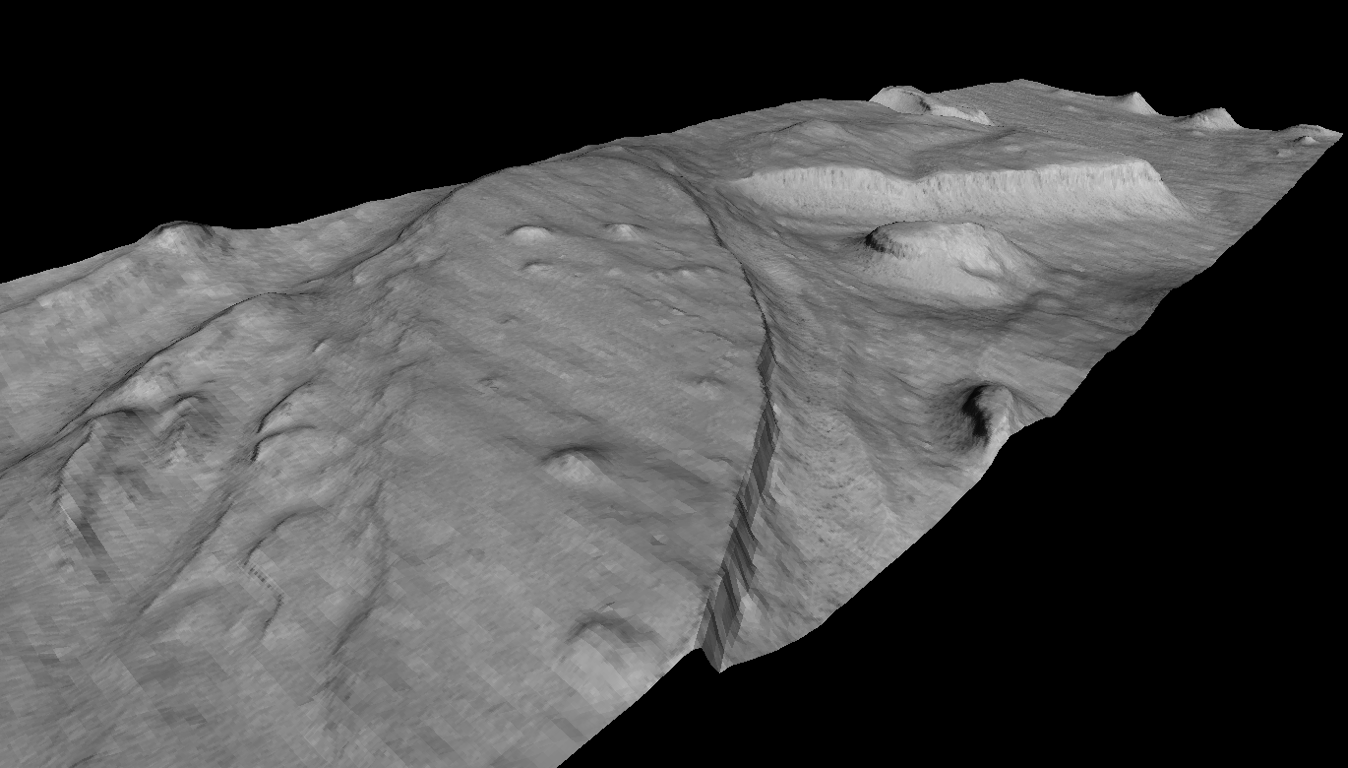
\includegraphics[width=6.5in]{images/introduction/p19view2.png}
   \caption{This 3D model was generated from a \acf{MOC} image
     pair M01/00115 and E02/01461 (34.66N, 141.29E).  The complete
     stereo reconstruction process takes approximately thirty minutes on
     a 3.0~GHz workstation for input images of this size ($1024 \times 8064$
     pixels).  This model, shown here without vertical
     exaggeration, is roughly 2~km wide in the cross-track
     dimension. }
   \label{fig:p19}
\end{figure}

\section{Background}

The \ac{IRG} at the NASA Ames Research Center has been developing
3D surface reconstruction and visualization capabilities for planetary
exploration for more than a decade.  First demonstrated during the
Mars Pathfinder Mission, the \ac{IRG} has delivered tools providing
these capabilities to the science operations teams of the Mars Polar
Lander (MPL) mission, the \ac{MER} mission, the \ac{MRO} mission,
and most recently the \ac{LRO} mission. A critical component
technology enabling this work is the \acf{ASP}.  The Stereo Pipeline
generates high quality, dense, texture-mapped 3D surface models
from stereo image pairs.

Although initially developed for ground control and scientific
visualization applications, the Stereo Pipeline has evolved in recent
years to address orbital stereogrammetry and cartographic
applications.  In particular, long-range mission planning requires
detailed knowledge of planetary topography, and high resolution
topography is often derived from stereo pairs captured from orbit.
Orbital mapping satellites are sent as precursors to planetary bodies
in advance of landers and rovers.  They return a wealth of imagery and
other data that helps mission planners and scientists identify areas
worthy of more detailed study. Topographic information often plays a
central role in this planning and analysis process.

Our recent development of the Stereo Pipeline coincides with a
period of time when \ac{NASA} orbital mapping missions are returning
orders of magnitude more data than ever before.  Data volumes from
the Mars and Lunar Reconnaissance Orbiter missions now measure in
the tens of Terabytes.  There is growing consensus that existing
processing techniques, which are still extremely human intensive
and expensive, are no longer adequate to address the data processing
needs of \ac{NASA} and the Planetary Science community.  To pick
an example of particular relevance, the \ac{HiRISE} instrument has
captured a few thousand stereo pairs.
Of these, only about a hundred stereo pairs have been processed to
date; mostly on human-operated, high-end photogrammetric workstations.
It is clear that much more value could be extracted from this
valuable raw data if a more streamlined, efficient process could be
developed.

The Stereo Pipeline was designed to address this very need.  By
applying recent advances in robotics and computer vision, we have
created an {\em automated} process that is capable of generating high
quality \acp{DEM} with minimal human intervention.  Users of the Stereo
Pipeline can expect to spend some time picking a handful of settings
when they first start processing a new type of imagery, but once this
is done the Stereo Pipeline can be used to process tens, hundreds, or
even thousands of stereo pairs without further adjustment.  With the
release of this software, we hope to encourage the adoption of this
tool chain at institutions that run and support these remote sensing
missions.  Over time, we hope to see this tool incorporated into
ground data processing systems alongside other automated image
processing pipelines.  As this tool continues to mature, we believe
that it will be capable of producing digital elevation models of
exceptional quality without any human intervention.

\section{Human vs. Computer: When to Choose Automation?}

When is it appropriate to choose automated stereo mapping over the use
of a conventional, human-operated photogrammetric workstation?  This
is a philosophical question with an answer that is likely to evolve
over the coming years as automated data processing technologies become
more robust and widely adopted.  For now, our opinion is that you
should {\em always} rely on human-guided, manual data processing
techniques for producing mission critical data products for missions
where human lives or considerable capital resources are at risk.  In
particular, maps for landing site analysis and precision landing
absolutely require the benefit of an expert human operator to
eliminate obvious errors in the \ac{DEM}; and also to guarantee that the
proper procedures have been followed to correct satellite telemetry
errors so that the data have the best possible geodetic control.

When it comes to using \acp{DEM} for scientific analysis, both techniques
have their merits.  Human-guided stereo reconstruction produces \acp{DEM}
of unparalleled quality that benefit from the intuition and experience
of an expert.  The process of building and validating these \acp{DEM} is
well established and accepted in the scientific community.

However, only a limited number of \acp{DEM} can be processed to this level
of quality.  For the rest, automated stereo processing can be used to
produce \acp{DEM} at a fraction of the cost.  The results are not
necessarily less accurate than those produced by the human operator,
but they will not benefit from the same level of scrutiny and quality
control.  As such, users of these \acp{DEM} must be able to identify
potential issues, and be on the lookout for errors that may result
from the improper use of these tools.

We recommend that all users of the Stereo Pipeline take the time to
thoroughly read this documentation and build an understanding of how
stereo reconstruction and bundle adjustment can be best used together to
produce high quality results. You are welcome to contact us if you have
any questions (section \ref{get-help}).

\section{Software Foundations}

\subsection{NASA Vision Workbench}

The Stereo Pipeline is built upon the Vision Workbench software
which is a general purpose image processing and computer vision
library also developed by the \ac{IRG}.  Some of the tools discussed
in this document are actually Vision Workbench programs, but any
distribution of the Stereo Pipeline requires the Vision Workbench.
Unless you're compiling the Vision Workbench and Stereo Pipeline from
source, the distinctions probably won't matter to you.


\subsection{The USGS Integrated Software for Imagers and Spectrometers}

For processing non-terrestrial NASA satellite imagery, Stereo Pipeline
must be installed alongside a copy of \ac{USGS} \ac{ISIS}. \ac{ISIS} is
however not required for processing Digital Globe images of Earth, as
described in section \ref{quickstartDG}.

\ac{ISIS} is widely used in the planetary science community
for processing raw spacecraft imagery into high level data products of
scientific interest such as map-projected and mosaicked imagery
\cite{2004LPI....35.2039A, 1997LPI....28..387G, ISIS_website}.  We
chose \ac{ISIS} because (1) it is widely adopted by the planetary
science community, (2) it contains the authoritative collection of
geometric camera models for planetary remote sensing instruments, and
(3) it is open source software that is easy to leverage.

By installing the Stereo Pipeline, you will be adding an advanced
stereo image processing capability that can be used in your existing
\ac{ISIS} workflow.  The Stereo Pipeline supports the \ac{ISIS}
``cube'' (\texttt{.cub}) file format, and can make use of the \ac{ISIS}
camera models and ancillary information (i.e. SPICE kernels) for
imagers on many \ac{NASA} spacecraft.  The use of this single standardized
set of camera models ensures consistency between products generated
in the Stereo Pipeline and those generated by \ac{ISIS}.  Also by
leveraging \ac{ISIS} camera models, the Stereo Pipeline can process
stereo pairs captured by just about any \ac{NASA} mission.


%% It might be good to add a section on terminology someday...
%\section{Terminology}
%
%DISPARTY
%
%TRIANGULATION
%
%CORRELATION
%
%BUNDLE ADJUSTMENT

\pagebreak
\section{Getting Help}\label{get-help}

All bugs, feature requests, and general discussion should be sent to
the Ames Stereo Pipeline user mailing list:
\begin{quote}
\indent \href{mailto:stereo-pipeline@lists.nasa.gov}{stereo-pipeline@lists.nasa.gov}
\end{quote}
To subscribe to this list, send an empty email message with the
subject `subscribe' (without the quotes) to:
\begin{quote}
\indent \href{mailto:stereo-pipeline-request@lists.nasa.gov}{stereo-pipeline-request@lists.nasa.gov}
\end{quote}
To contact the lead developers and project manager directly, send mail
to:
\begin{quote}
\indent \href{mailto:stereo-pipeline-owner@lists.nasa.gov}{stereo-pipeline-owner@lists.nasa.gov}
\end{quote}

\section{How to File Bug Reports} 

If Stereo Pipeline crashes or produces incorrect results, we would very
much like to hear from you. You can send an email to
\texttt{stereo-pipeline-owner@lists.nasa.gov} describing the problem. It
will be helpful to attach the logs output by \texttt{stereo} and other
tools (section \ref{logging}). In some cases we may request your input
data as well.

\section{Typographical Conventions}

Names of programs that are meant to be run on the command line are
written in a constant-width font, like the \texttt{stereo} program,
as are options to those programs.

An indented line of constant-width text can be typed into your
terminal, these lines will either begin with a `\texttt{>}' to
denote a regular shell, or with `\texttt{ISIS}' which denotes an
\ac{ISIS}-enabled shell (which means you have to set the \texttt{ISISROOT}
environment variable and sourced the appropriate \ac{ISIS} 3 Startup
script, as detailed in the \ac{ISIS} 3 instructions).
\begin{verbatim}
  > ls

  ISIS 3> pds2isis
\end{verbatim}

Italicized constant-width text denotes an option or argument that
a user will need to supply.  For example, `\texttt{stereo E0201461.map.cub
M0100115.map.cub out}' is specific, but `\texttt{stereo \textit{left-image
right-image} out}' indicates that \texttt{\textit{left-image}} and
\texttt{\textit{right-image}} are not the names of specific files,
but dummy parameters which need to be replaced with actual file
names.

Square brackets denote optional options or values to a command, and
items separated by a vertical bar are either aliases for each other, or
different, specific options.  Default arguments are prefixed by an equals
sign within parentheses, and line continuation with a backslash:

\texttt{  point2dem [-\/-help|-h] [-r moon|mars] [-s \textit{float(=0)}] $\backslash$ } \\
\hspace*{6em}\texttt{[-o \textit{output-filename}] \textit{pointcloud}-PC.tif}

The above indicates a run of the \texttt{point2dem} program.  The
only argument that it requires is a point cloud file, which is
produced by the \texttt{stereo} program and ends in \texttt{-PC.tif},
although its prefix could be anything (hence the italics for that
part).  Everything else is in square brackets indicating that they
are optional.

Both \texttt{-\/-help} and \texttt{-h} are really the same thing (both
will get you help).  Similarly, the argument to the \texttt{-r}
option must be either \texttt{moon} or \texttt{mars}.  The \texttt{-s}
option takes a floating point value as its argument, and has a
default value of zero.  The \texttt{-o} option takes a filename
that will be used as the output \ac{DEM}.

Although there are two lines of constant-width text, the backslash at the end
of the first line indicates that the command continues on the second line.  You
can either type everything into one long line on your own terminal, or use the
backslash character (or appropriate line continuation character) and a return to
continue typing on a second line in your terminal.


\section{Referencing the Ames Stereo Pipeline in Your Work}

Although no peer-reviewed paper or report yet exists which details the
Ames Stereo Pipeline (see the warning below about this being {\bf
  research} software), if you do use this software in your work, we'd
appreciate it if you referenced one or more of these abstracts:

\begin{description}
\item Moratto, Z. M., M. J. Broxton, R. A. Beyer, M. Lundy, and K. Husmann.
2010. Ames Stereo Pipeline, NASA's Open Source Automated Stereogrammetry
Software. \textit{Lunar and Planetary Science Conference} \textbf{41},
abstract \#2364.
\href{http://adsabs.harvard.edu/abs/2010LPI....41.2364M}{[ADS Abstract]}.

\item Broxton, M. J. and L. J. Edwards. 2008. The Ames Stereo Pipeline:
Automated 3D Surface Reconstruction from Orbital Imagery. \textit{Lunar
and Planetary Science Conference} \textbf{39}, abstract \#2419.
\href{http://adsabs.harvard.edu/abs/2008LPI....39.2419B}{[ADS Abstract]}.
\end{description}

\section{Warnings to Users of the Ames Stereo Pipeline}

Ames Stereo Pipeline is a {\bf research} product. There may be bugs or
incomplete features. We reserve the ability to change the API and
command line options of the tools we provide. Although we hope you will
find this release helpful, you may use it at your own risk. Please check
each release's {\bf NEWS} file to see a summary of our recent changes.

While we are confident that the algorithms used by this software are
robust, they have not been systematically tested or rigorously
compared to other methods in the peer-reviewed literature. We have a
number of efforts underway to carefully compare Stereo
Pipeline-generated data products to those produced using established
processes, and we will publish those results as they become available.
In the meantime, we {\it strongly recommend} that you consult us first
before publishing any results based on the cartographic products
produced by this software.


\part{Getting Started}
\chapter{Installation}

\section{Binary Installation}

This is the recommended method. Only two things are required:

\begin{description}
\item [{Stereo~Pipeline~tarball.}] The main Stereo Pipeline page is \url{http://ti.arc.nasa.gov/stereopipeline}.
In the upper-right, there is a list of files. Download the \emph{Binary}
option that matches the platform you wish to use. The required \ac{ISIS}
version is listed next to the name; choose the newest version you
have available.

\item [{\ac{USGS}~\ac{ISIS}~Binary~Distribution.}] The Stereo Pipeline depends
on \ac{ISIS} version 3 from the USGS\@. Their installation guide is at \url{http://isis.astrogeology.usgs.gov/documents/InstallGuide}.
You must use their binaries as-is; if you need to recompile, you must
follow the \emph{Source Installation} guide in Section~\ref{sec:Source-Installation}.
Note also that the \ac{USGS} does not provide any version of \ac{ISIS} but the
current one. If you need a past version, you must retain it yourself.
\end{description}

\subsection{Quickstart}
\begin{description}

\item[{Fetch~Stereo~Pipeline}] ~\\
Download the Stereo Pipeline from \url{http://ti.arc.nasa.gov/stereopipeline}.

\item [{Fetch~\ac{ISIS}\_Binaries}] ~\\
\verb#rsync -azv --delete isisdist.wr.usgs.gov::isis3_ARCH_OS/isis .#

\item [{Fetch~\ac{ISIS}\_Data}] ~\\
\verb#rsync -azv --delete isisdist.wr.usgs.gov::isis3data/data .#

\item [{Untar~\acl{ASP}}] ~\\
\verb#tar xzvf StereoPipeline-VERSION-ARCH-OS.tar.gz#

% Verbatim has way too much white space. Couldn't seem to take care of it with
% vskip/vspace negative. Sigh.
\item [{Add~Stereo~Pipeline~to~Path~(optional)}] ~\\
\verb#(bash) export PATH="/path/to/StereoPipeline/bin:${PATH}"# \\
\verb#(csh)  setenv PATH "/path/to/StereoPipeline/bin:${PATH}"#

% Grrrr. Why doesn't it keep this together? Sprinkling in \nopagebreak
% doesn't seem to work... Forcing a pagebreak instead
\pagebreak
\item[Set~Up~Isis] ~\\
\verb#(bash)# \\
\verb#    export ISISROOT=/path/to/isisroot# \\
\verb#    source $ISISROOT/scripts/isis3Startup.sh# \\
\verb#(csh)# \\
\verb#    setenv ISISROOT /path/to/isisroot# \\
\verb#    source $ISISROOT/scripts/isis3Startup.csh#

\item [{Try~It~Out!}] ~\\
See the next chapter (Chapter~\ref{ch:tutorial}) for an example!
\end{description}

\subsection{Common Traps}

Here are some errors you might see, and what it could mean. Treat
these as templates for problems--- in practice, the error messages might
be slightly different.

\begin{verbatim}
stereo: error while loading shared libraries: libisis3.so:
    cannot open shared object file: No such file or directory
\end{verbatim}

You just need to set up your ISIS environment.

\begin{verbatim}
dyld: Library not loaded: $ISISROOT/lib/libisis3.dylib
Referenced from: /some/path/goes/here/bin/program
Reason: image not found Trace/BPT trap
\end{verbatim}

You just need to set up your ISIS environment.

\begin{verbatim}
point2mesh E0201461-M0100115-PC.tif E0201461-M0100115-L.tif
[...]
99%  Vertices:   [************************************************************] Complete!
       > size: 82212 vertices
Drawing Triangle Strips
Attaching Texture Data
zsh: bus error  point2mesh E0201461-M0100115-PC.tif E0201461-M0100115-L.tif
\end{verbatim}

The source of this problem is an old version of OpenSceneGraph in
your library path. Check your \verb#LD_LIBRARY_PATH# (for Linux),
\verb#DYLD_LIBRARY_PATH# (for OSX), or your \verb#DYLD_FALLBACK_LIBRARY_PATH#
(for OSX) to see if you have an old version listed, and remove if
from the path if that is the case. It is not necessary to remove the
old versions from your computer, you just need to remove the reference
to them from your library path.

\section{\label{sec:Source-Installation}Source Installation}

This method is for advanced users only.

\subsection{Dependency List}

This is a list of direct dependencies of Stereo Pipeline. Some libraries
(like ISIS) have dependencies of their own which are not covered here.

\begin{description}
\item [{Boost}] (Required) \url{http://www.boost.org/}\\
Version 1.35 or greater is required. Along with the base library
set, the Stereo Pipeline specifically requires: Program Options, Filesystem,
Thread, and Graph.

\item [{LAPACK}] (Required)\\
There are many sources for LAPACK\@. For OSX, you can use the
vecLib framework. For Linux, you can use the netlib LAPACK/CLAPACK
distributions, or Intel's MKL, or any of a number of others. The math
is unfortunately not a hotspot in the code, though, so using a faster
LAPACK implementation will not change much. Therefore, you should
probably just use the LAPACK your package manager (RPM for Red Hat
Linux, Yast for SuSE, etc.) has available.

\item [{ISIS}] (Recommended) \url{http://isis.astrogeology.usgs.gov/documents/InstallGuide}\\
The USGS Integrated Software for Imagers and Spectrometers (ISIS) library. This
library handles the camera models and image formats used for instruments.

\item [{OpenSceneGraph}] (Optional) \url{http://www.openscenegraph.org/}\\
OpenSceneGraph is required to run the \texttt{point2mesh} tool
(See Section~\ref{point2mesh}).

\item [{Vision~Workbench}] (Required) \url{http://ti.arc.nasa.gov/visionworkbench/}\\
Vision Workbench forms much of the core processing code of the
Stereo Pipeline.

\end{description}

\subsection{Build System}

The build system is built on GNU autotools. In-depth information on
autotools is available from \url{http://sources.redhat.com/autobook/}.
The basics, however, are simple. To compile the source code, first
run \verb#./configure# from the top-level directory. This will search
for the dependencies and enable the modules you requested. There are
a number of options that can be passed to \verb#configure#; many
of these options can also be placed into a \verb#config.options#
file (in the form of \verb#VARIABLE="VALUE"#) in the same directory
as \verb#configure#. Table \ref{tab:Supported-configure-options}
lists the supported options.

\begin{table}
\begin{longtable}{|l|l|c|m{5cm}|}
\hline
\textbf{Variable Name}                & \textbf{Configure option}               & \textbf{Default} & \textbf{Function}\tabularnewline
\hline
\hline
\small\verb#PREFIX#                   & \small\verb#--prefix#                   & /usr/local       & Set the install prefix (ex: binaries will go in \$PREFIX/bin)\tabularnewline
\hline
\small\verb#HAVE_PKG_XXX#             & \small\verb#--with-xxx#                 & auto             & Set to {}``no'' to disable package XXX, or a path to only search that path\tabularnewline
\hline
\small\verb#PKG_PATHS#                & \small\verb#--with-pkg-paths#           & many             & Prepend to default list of search paths\tabularnewline
\hline
\small\verb#ENABLE_PKG_PATHS_DEFAULT# & \small\verb#--enable-pkg-paths-default# & yes              & Append built-in list of search paths\tabularnewline
\hline
\small\verb#ENABLE_OPTIMIZE#          & \small\verb#--enable-optimize#          & 3                & Level of compiler optimization?\tabularnewline
\hline
\small\verb#ENABLE_DEBUG#             & \small\verb#--enable-debug#             & no               & How much debug information?\tabularnewline
\hline
\small\verb#ENABLE_CCACHE#            & \small\verb#--enable-ccache#            & no               & Use \verb#ccache# if available\tabularnewline
\hline
\small\verb#ENABLE_RPATH#             & \small\verb#--enable-rpath#             & no               & Set RPATH on built binaries and libraries\tabularnewline
\hline
\small\verb#ENABLE_ARCH_LIBS#         & \small\verb#--enable-arch-libs#         & no               & Pass in 64 or 32 to look for libraries by default in \verb#lib64# or \verb#lib32#\tabularnewline
\hline
\small\verb#ENABLE_PROFILE#           & \small\verb#--enable-profile#           & no               & Use function profiling?\tabularnewline
\hline
\small\verb#PKG_XXX_CPPFLAGS#         &                                         &                  & Append value to CPPFLAGS for package XXX\tabularnewline
\hline
\small\verb#PKG_XXX_LDFLAGS#          &                                         &                  & Prepend value to LDFLAGS for package XXX\tabularnewline
\hline
\small\verb#PKG_XXX_LIBS#             &                                         &                  & Override the required libraries for package XXX\tabularnewline
\hline
\small\verb#PKG_XXX_MORE_LIBS#        &                                         &                  & Append to required libraries for package XXX\tabularnewline
\hline
\small\verb#ENABLE_EXCEPTIONS#        & \small\verb#--enable-exceptions#        & yes              & Use C++ exceptions? Disable at own risk.\tabularnewline
\hline
\small\verb#ENABLE_MULTI_ARCH#        & \small\verb#--enable-multi-arch#        & no               & OSX Only: Build \emph{Fat} binary with space-separated list of arches\tabularnewline
\hline
\small\verb#ENABLE_AS_NEEDED#         & \small\verb#--enable-as-needed#         & no               & Pass --as-needed to GNU linker. Use at your own risk.\tabularnewline
\hline
\end{longtable}\caption{\label{tab:Supported-configure-options}Supported configure options}
\end{table}

\end{document}

\chapter{Tutorial: Processing Mars Orbiter Camera Imagery}
\label{ch:tutorial}

\section{Quick Start}

The programs in the Stereo Pipeline are command-line programs which
take a pair of images, and attempt to create a three-dimensional
point cloud from correlating them.  Then there are a few programs
that can convert that point cloud into a mesh for viewing or a
gridded terrain model for use in other ways.

So at the highest, most abstract level, if you have two image files
(say \texttt{image\_file1} and \texttt{image\_file2} ) this command
makes point clouds (and a bunch of other files):

\begin{verbatim}
    stereo image_file1 image_file2 stereo-output
\end{verbatim}
\noindent
Then you can make a mesh or a DEM file with either of the following
commands.  The \texttt{stereo-output-PC.tif} and
\texttt{stereo-output-L.tif} files are created by the \texttt{stereo}
program run above):

\begin{verbatim}
    point2mesh stereo-output-PC.tif stereo-output-L.tif

    point2dem stereo-output-PC.tif stereo-output-L.tif
\end{verbatim}
\noindent
There are a number of ways to fine-tune parameters and
analyze the results, but ultimately this software suite takes images
and builds models in a mostly automatic way.

% \section{Examples of Use}
%
% Download the tarball and it will unpack into a \texttt{p19} directory.  Create an output directory to hold the results, and invoke the \texttt{stereo} program:
%
% \begin{verbatim}
%       mkdir results
%       stereo E0201461.cub M0100115.cub results/p19
% \end{verbatim}
%
% You can look at the results by examining the disparity images. These
% show the horizontal and vertical components of the matching offsets
% for each pixel, and they can be a useful debugging tool if you want
% to check how the stereo matcher performed for a given stereo pair:
%
% \begin{verbatim}
%       cd results
%       disparitydebug p19-D.exr -o p19-D
%       disparitydebug p19-F.exr -o p19-F
% \end{verbatim}
%
% \emph{MJB: What exactly is being examined in the resultant images, what are users looking for?}
%
% A 3D mesh can be built from the point cloud and viewed using the
% \texttt{osgviewer} program:
%
% \begin{verbatim}
%       point2mesh p19-PC.tif p19-L.tif -o p19
%       osgviewer p19.ive
% \end{verbatim}
%
% When the \texttt{osgviewer} starts, you may want to turn off the
% lighting (hit the `L' key).
%
% A gridded DEM with floating point pixels can also be built from the point cloud:
%
% \begin{verbatim}
%       point2dem --xyz-to-lonlat -r mars p19-PC.tif -n -o p19
% \end{verbatim}
%
% You can also orthoproject the raw satellite imagery onto the DEM during this step:
%
% \begin{verbatim}
%       point2dem --xyz-to-lonlat -r mars p19-PC.tif -o p19 --orthoimage p19-L.tif
% \end{verbatim}
%
% Finally, you can create colorized, shaded relief (or both) images from the DEM, using these Vision Workbench programs:
%
% \begin{verbatim}
%       colormap p19-DEM.tif -o p19-colorized.tif
%       hillshade p19-DEM.tif -o p19-shaded.tif -e 25
%       colormap p19-DEM.tif --shaded-relief-file p19-shaded.tif -o p19-color-shaded.tif
% \end{verbatim}
%
% Finally, you can run the Vision Workbench's \texttt{image2qtree} on any of the following files:
%
% \begin{itemize}
% \item p19-DEM-normalized.tif
% \item p19-DRG.tif
% \item p19-shaded.tif
% \item p19-colorized.tif
% \item p19-shaded-colorized.tif
% \end{itemize}


\section{Preparing the Data}

The data set that is used in the tutorial and examples below is a pair
of Mars Orbiter Camera (MOC)
\citep{1992JGR....97.7699M,2001JGR...10623429M} images whose Planetary
Data System (PDS) Product IDs are M01/00115 and E02/01461.  These data
can be downloaded from the PDS directly, or they can be found in the
\texttt{data/MOC/} directory of your Stere Pipeline distribution.

These raw PDS images (\texttt{M0100115.imq} and \texttt{E0201461.imq})
need to be imported into the ISIS environment and radiometrically
calibrated.  You will need to be in an ISIS environment (have set the
\texttt{ISISROOT} environment variable and sourced the appropriate
ISIS 3 Startup script, as detailed in the ISIS 3 instructions, we will
denote this state with the `\texttt{ISIS 3>}' prompt).  Then you can
use the \texttt{mocproc} program.

\begin{verbatim}
    ISIS 3> mocproc from= M0100115.imq to= M0100115.cub Mapping= NO
\end{verbatim}
\noindent
There are also \texttt{Ingestion} and \texttt{Calibration} parameters
whose defaults are `\texttt{YES}' which will bring the image into
the ISIS format and perform radiometric calibration.  By setting
the \texttt{Mapping} parameter to `\texttt{NO}' the resultant file
will be an ISIS cube file that is calibrated, but not map-projected.
Note that while we have not explicitly run \texttt{spiceinit}, the
Ingestion portion of \texttt{mocproc} quietly ran \texttt{spiceinit}
for you (you'll find the record of it in the ISIS Session Log,
usually written out to a file named \texttt{print.prt}).

\begin{figure}[b!]
\begin{minipage}{5.2in}
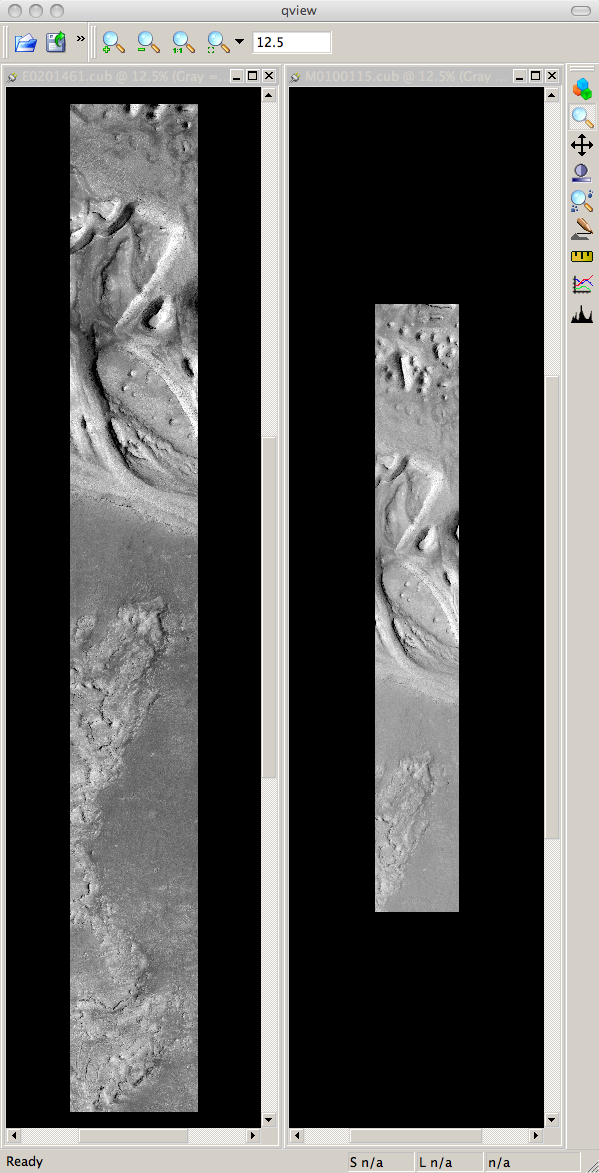
\includegraphics[height=3.7in]{images/p19-images.png}
\hfill
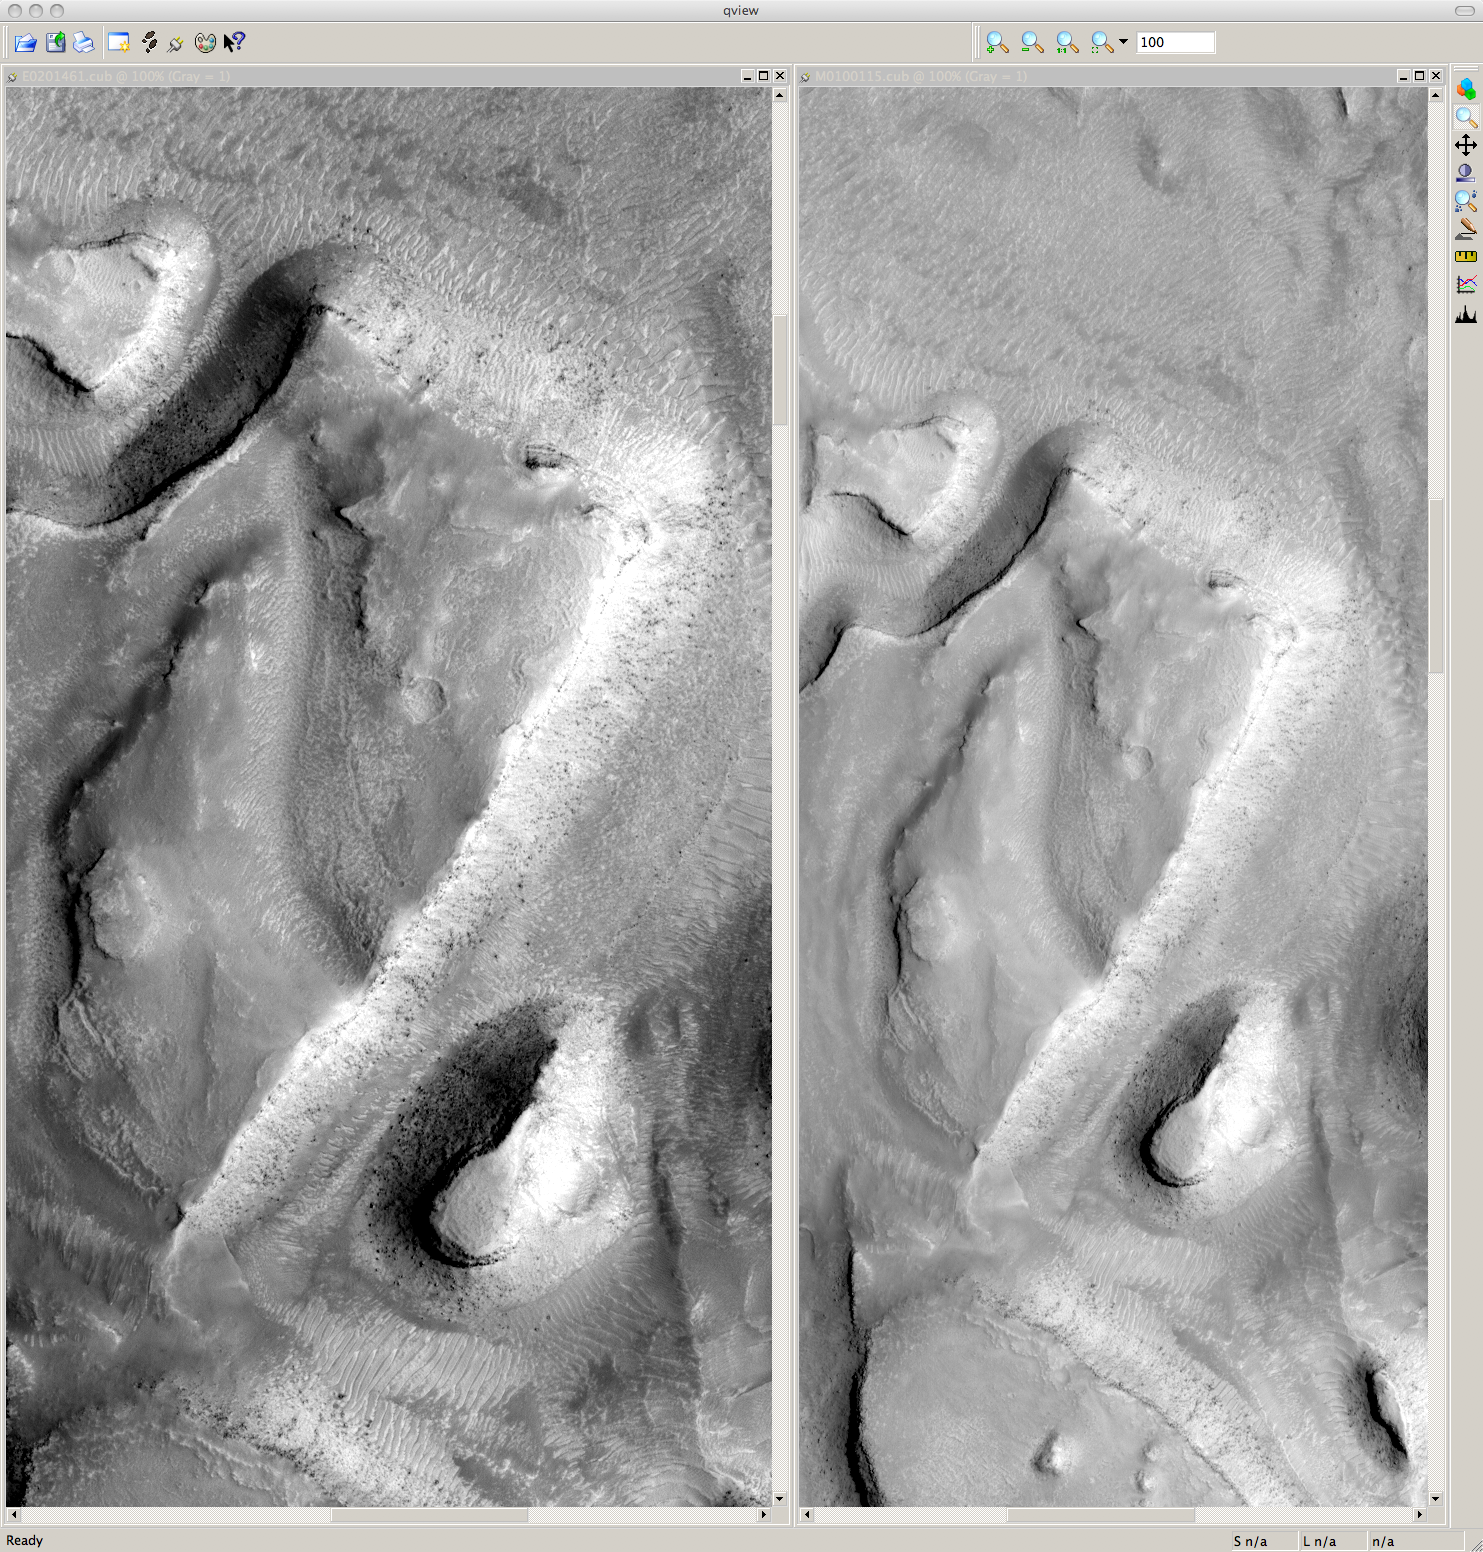
\includegraphics[height=3.7in]{images/p19-images_zoom.png}
\end{minipage}
\hfill
\begin{minipage}{1.3in}
\caption[P19 images open in qview zoomed in]{
    \label{p19-images}
    This figure shows \texttt{E0201461.cub} and \texttt{M0100115.cub}
    open in ISIS's qview program.  The view on the left shows their
    full extents at the same zoom level, showing how they have
    different ground scales.  The view on the right shows both images
    zoomed in on the same feature.  }
\end{minipage}
\end{figure}

\section{Running the Stereo Pipelinex}

The following example will utilize images from the example MOC
dataset, discussed above.  The two example ISIS 3 image files are
\texttt{E0201461.cub} and \texttt{M0100115.cub}.

The \texttt{stereo} program (page \pageref{stereo}) is designed for
automated tie point matching and stereo production, and is the first
Stereo Pipeline tool we'll use.

If you like, you should create a directory for the results of the
processing.  The \texttt{stereo} program can generate a number of
output files, and we find it helpful to put them all in a directory,
but it isn't required.

\begin{verbatim}
    > ls
    E0201461.cub   M0100115.cub
    > mkdir results
\end{verbatim}
\noindent
The \texttt{stereo} program requires a \texttt{stereo.default} file
which can be altered for your needs.  Its contents are detailed on
page \pageref{stereo.default}.  You may find it useful to save
multiple versions of the \texttt{stereo.default} file for various
processing needs. If you need to do that, be sure to specify which
configuration file \texttt{stereo} should use with the \texttt{-s}
option.  If this option is not given, the \texttt{stereo} program
will search for a file named \texttt{stereo.default} in the current
directory and will complain if there isn't one.

There is a \texttt{stereo.default} file included with the example
data set that is different from the example \texttt{stereo.default.example}
file distributed with the Stereo Pipeline.  The \texttt{stereo.default}
included with the example data set has a smaller correlation window
(smaller values for the \texttt{H\_CORR\_*} and \texttt{V\_CORR\_*}
variables) that is more suited to the MOC data.  You may want to
use both this \texttt{stereo.default} and the
\texttt{stereo.default.example} to explore how the results are
different.

Alternatively, it is possible to not have to define the
\texttt{H\_CORR\_*} and \texttt{V\_CORR\_*} is
\texttt{stereo.default}. When this happens, \texttt{stereo} will
collect interest points on reduced version of the input to guess the
correct search range. \texttt{stereo} prints it's guess in the command
window and it can be used a starting point if the results don't turn
out.

So run \texttt{stereo} like this (there should be a
\texttt{stereo.default} file distributed along with the example
data set that will be used):

\begin{verbatim}
    ISIS 3> stereo E0201461.cub M0100115.cub results/E0201461-M0100115
\end{verbatim}

\noindent
That last option (\emph{results/E0201461-M0100115}) can be anything you
want it to be.  It designates the text that \texttt{stereo} will use
as a prefix for its many output files.  Since the first part is
\texttt{results/} this causes the program to put the results in that
directory with files whose names start with
\texttt{E0201461-M0100115}. If instead that last text was just
\texttt{E0201461-M0100115} it would have created a bunch of files that
start with \texttt{E0201461-M0100115} in the same directory as the
input files.

The \texttt{stereo} program's processing moves through several
stages which are detailed on page \pageref{entrypoints}.  However,
once the \texttt{stereo} program completes, it creates a number of
files.  A quick look at some of the TIFF files created, can quickly
give you an idea of what the \texttt{stereo} program did (figure
\ref{p19-stereo-output}).

\begin{figure}
\begin{center}
\includegraphics[width=5in]{images/p19-stereo-output.png}
\caption[P19 stereo output images]{
    \label{p19-stereo-output}
	These are the four viewable \texttt{.tif} files created by
	the \texttt{stereo} program.  The left two are the aligned
	images (\texttt{E0201461-M0100115-L.tif} and
	\texttt{E0201461-M0100115-R.tif}).  The next two images are
	the mask images (\texttt{E0201461-M0100115-lMask.tif} and
	\texttt{E0201461-M0100115-rMask.tif}), which indicate which
	pixels in the aligned images are good to use for the next
	step.  The image on the right is the Good Pixel map
	(\texttt{E0201461-M0100115-GoodPixelMap.tif}), which indicates
	the pixels in grey which were successfully matched with the
	correlator.  The red pixels were not.  Those red pixels which
	are not black in both mask images are optionally filled later
	during the hole-filling step.
    }
\end{center}
\end{figure}

% \begin{figure}
% \begin{center}
% 
\includegraphics[height=8in]{images/p19-goodpixel.png}
% \caption[P19 good pixel image]{
%     \label{p19-goodpixel}
% 	The Good Pixel map.
% 	Red pixels are not useful for alignment.
%     }
% \end{center}
% \end{figure}
%
% \begin{figure}
% \begin{center}
% 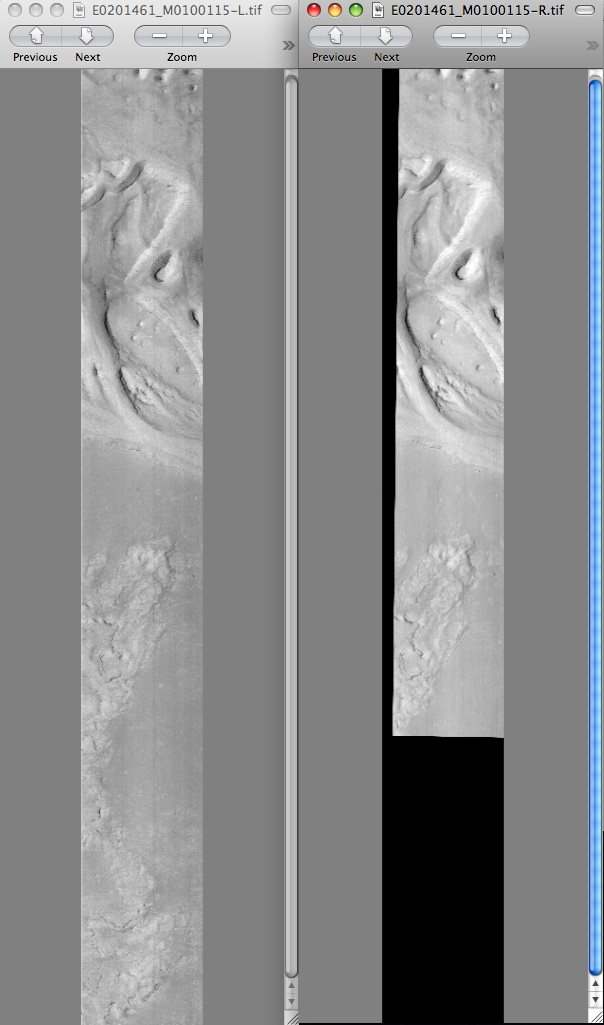
\includegraphics[width=3in]{images/p19-aligned.png}
% \caption[P19 aligned image]{
%     \label{p19-aligned}
% 	The left and right aligned images.
%     }
% \end{center}
% \end{figure}

If those TIFF files look okay, you can probably just go on to making
a mesh or a DTM from the point cloud file
(\texttt{E0201461-M0100115-PC.tif}).  The most important file is
the Good Pixel Map (\texttt{E0201461-M0100115-GoodPixelMap.tif}).
If this file shows mostly good, gray pixels in the overlap area
(the area that is white in both the \texttt{E0201461-M0100115-lMask.tif}
and \texttt{E0201461-M0100115-rMask.tif} files), then you're probably
good to go.  If this shows bad, red pixels in the overlap area,
then you'll probabaly need to go back and tune your \texttt{stereo.default}
file.  The example data also contains a \texttt{stereo.bad} file
which has intentionally bogus values for the dimensions of the
correlation window.  You can run \texttt{stereo} with the \texttt{-s
stereo.bad} command to see what the Good Pixel Map looks like with
this.

To get an idea of the disparity information that the \texttt{stereo}
program created and then used to build the point cloud, it can be
useful to take a look at that disparity information.  The \texttt{stereo}
program records this information in several \texttt{.exr} disparity
files.

To get a look at the disparity information, you need to convert it
into a more viewable format.  Move into the directory that contains
your results, and run the \texttt{disparitydebug} program (page
\pageref{disparitydebug}) to create the the horizontal and vertical
components of the disparity (matching offsets for each pixel).

\begin{figure}[b!]
\begin{minipage}{4in}
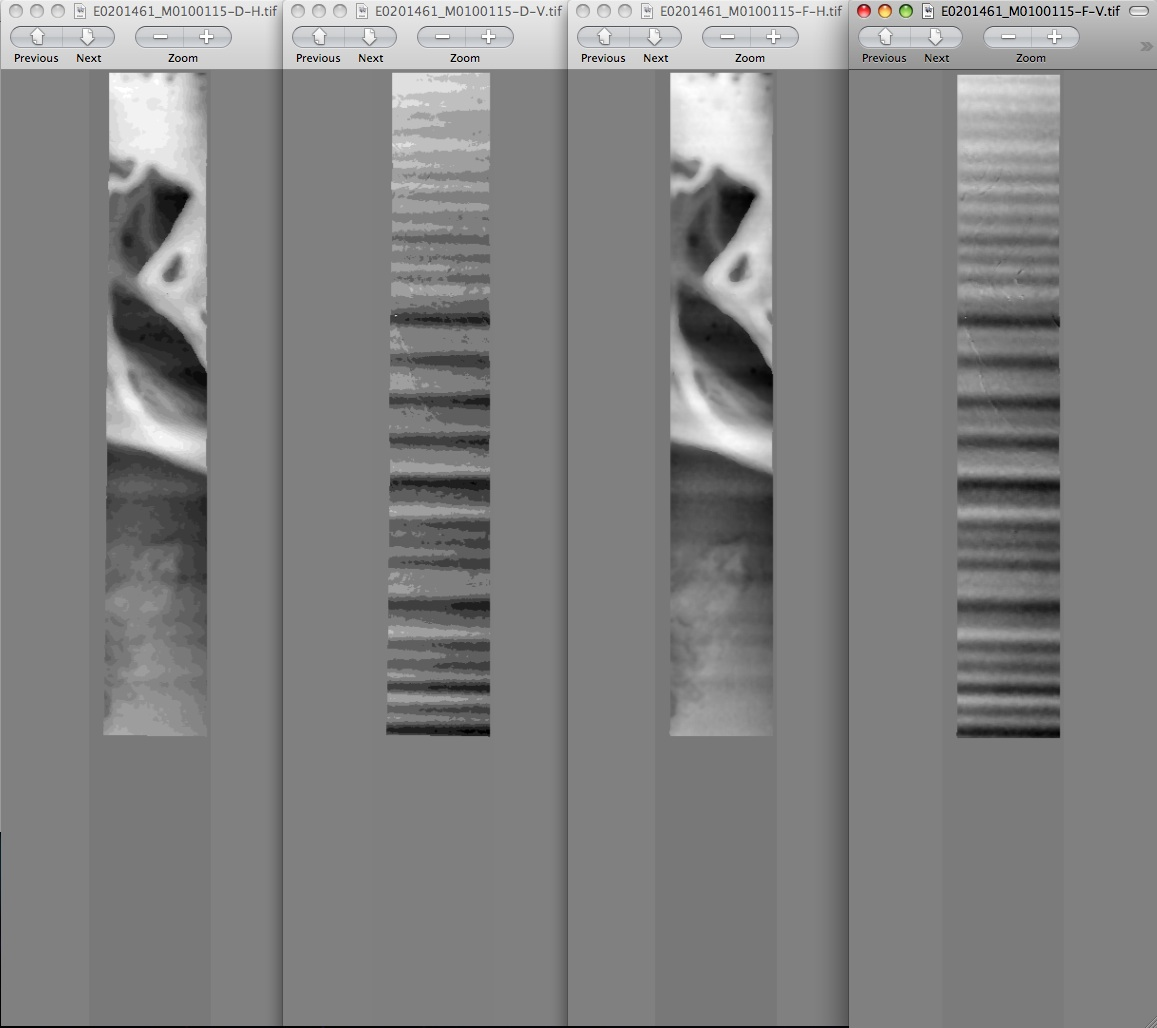
\includegraphics[width=4in]{images/p19-disparity.png}
\end{minipage}
\hfill
\begin{minipage}{2.7in}
\caption[P19 disparity images]{
    \label{p19-disparity}
	The disparity images.  The two images on the left are the
	\texttt{E0201461-M0100115-D-H.tif} and
	\texttt{E0201461-M0100115-D-V.tif} files, which are the raw horizontal and
	vertical disparity components.  The two images on the right are the
	\texttt{E0201461-M0100115-F-H.tif} and
	\texttt{E0201461-M0100115-F-V.tif} files, which are the final
	filtered, sub-pixel disparity map with outlier removal and holes
	filled in, and is what will be used to build the point cloud.  Since
	these MOC images were acquired by rolling the spacecraft across-track,
	most of the disparity that represents topography is present in the
	horizontal disparity map.  The vertical disparity map shows disparity
	not from topography, but from spacecraft movement.
    }
\end{minipage}
\end{figure}

\begin{verbatim}
    cd results
    disparitydebug E0201461-M0100115-F.exr
\end{verbatim}

\noindent
The two output files, \texttt{E0201461-M0100115-F-H.tif} and
\texttt{E0201461-M0100115-F-V.tif} are normalized images of the
horizontal (H) and vertical (V) disparity.  `Normalized' is a key
word here.  You can see that the horizontal and vertical disparity
images in figure \ref{p19-disparity} have the same range of gray
values from white to black, but they represent significantly different
absolute amounts of disparity.  These files are useful if you want
to check the performance of the \texttt{stereo} program for any
given stereo pair.

There are actually four flavors of disparity map: the \texttt{-D.exr},
the \texttt{-R.exr}, the \texttt{-F-corrected.exr}, and \texttt{-F.exr}.
You can run \texttt{disparitydebug} on any of them, and actually taking a
look at all of them can show you the differences between the disparity maps
at the different stages of processing.

\section{Visualizing the Results}

When \texttt{stereo} finishes up, it will have produced a point cloud.
At this point, the processing fans out, as many kinds of data
products can be built from the \texttt{E0201461-M0100115-PC.tif}.

One of the things that can be done is to produce a 3D mesh with
\texttt{point2mesh} (page \pageref{point2mesh}). This is not a science
product, but is just a quick visualization that can show the data
rendered in 3D. The mesh produced can be viewed with
\texttt{osgviewer} (the Open Scene Graph Viewer program, distributed
with the binary version of the Stereo Pipeline).  The
\texttt{point2mesh} program takes the point cloud file and the left
normalized image created by \texttt{stereo} as inputs.

\begin{verbatim}
    point2mesh E0201461-M0100115-PC.tif E0201461-M0100115-L.tif -l
\end{verbatim}

\noindent
This will create the file \texttt{E0201461-M0100115.ive}, openable
with \texttt{osgviewer}. When the \texttt{osgviewer} program starts,
you may want to turn off the lighting (hit the `L' key).

\begin{figure}[h]
\begin{minipage}{5in}
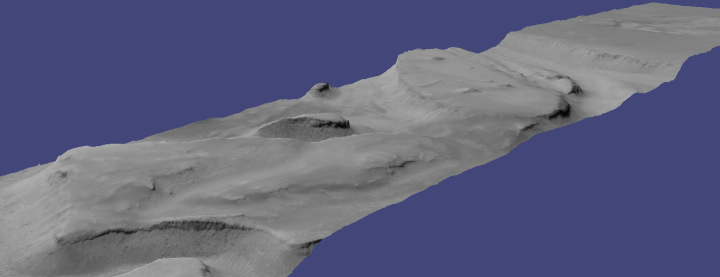
\includegraphics[width=5in]{images/p19-osg.png}
\end{minipage}
\hfill
\begin{minipage}{1.7in}
\caption[P19 in OSG]{
    \label{p19-osg}
	This shows the \texttt{E0201461-M0100115.ive} file displayed in
	the OSG Viewer.
    }
\end{minipage}
\end{figure}

The \texttt{point2dem} program (page \pageref{point2dem}) creates
a digital elevation model (DEM) from the Point Cloud file.

\begin{verbatim}
    point2dem E0201461-M0100115-PC.tif
\end{verbatim}

The resultant file, \texttt{E0201461-M0100115-DEM.tif}, will have
32-bit pixels, and so (much like the \texttt{E0201461-M0100115-PC.tif}
file) will not render well in typical image viewers. The resulting TIF
file is also contain georeferencing information which is useful for
working with other GIS platforms.

You can specify a coordinate system (e.g., latlon) and a reference
spheroid (i.e., calculated for the Moon or Mars). You also have the
option of creating a normalized DEM in addition to the automatically
generated non-normalized DEM. The normalized DEM again is just for
visualization and checking the quality of the product.

\begin{verbatim}
    point2dem --xyz-to-lonlat -r mars -n E0201461-M0100115-PC.tif
\end{verbatim}

\noindent
The \texttt{point2dem} program can also be used to orthoproject raw
satellite imagery onto the DEM. To do this, invoke \texttt{point2dem}
just as before, but add the \texttt{orthoimage} option and specify
the use of the left image file as the texture file to use for the
projection

\begin{verbatim}
    point2dem --xyz-to-lonlat -r mars --orthoimage E0201461-M0100115-L.tif \
      E0201461-M0100115-PC.tif
\end{verbatim}

\noindent
The \texttt{point2dem} program can be used in many different ways.
Be sure to explore all of the options.

\begin{figure}
\begin{minipage}{4in}
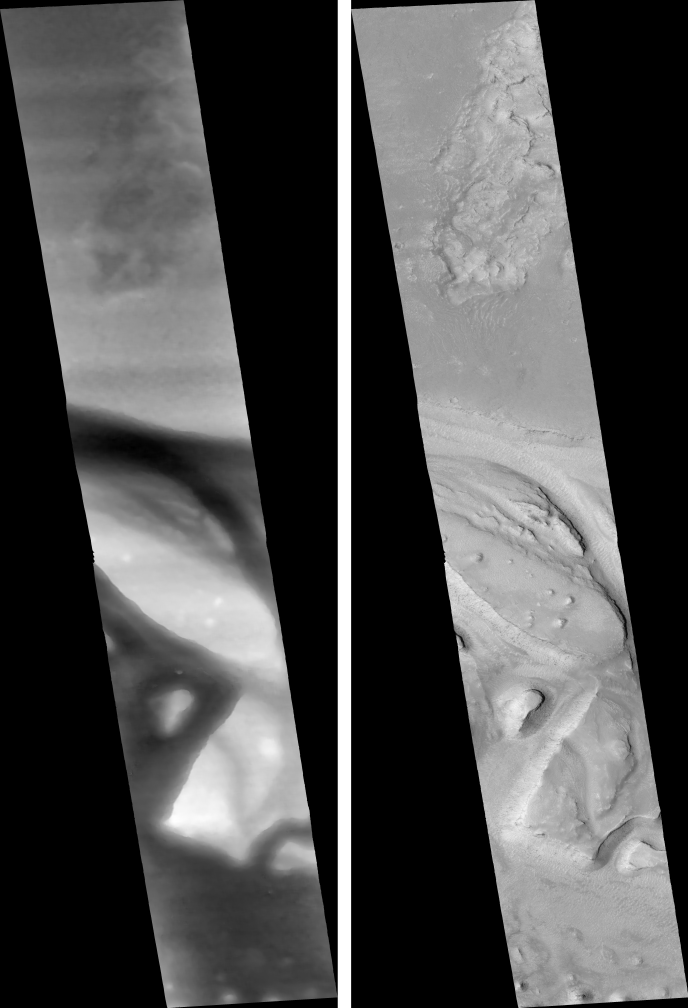
\includegraphics[width=4in]{images/p19-norm_ortho.png}
\end{minipage}
\hfill
\begin{minipage}{2.7in}
\caption[P19 Normalized DEM and Orthophoto]{
    \label{p19-norm_ortho}
	The image on the left is a normalized DEM (using the
	\texttt{-n} option) which which shows low terrain values
	as black and high terrain values as white (in a 0 to 255
	sense).  The image on the right is the orthographic image
	(created using the \texttt{--orthoimage} option to
	\texttt{point2dem}).
    }
\end{minipage} \end{figure}

% \begin{figure}
% \begin{center}
% 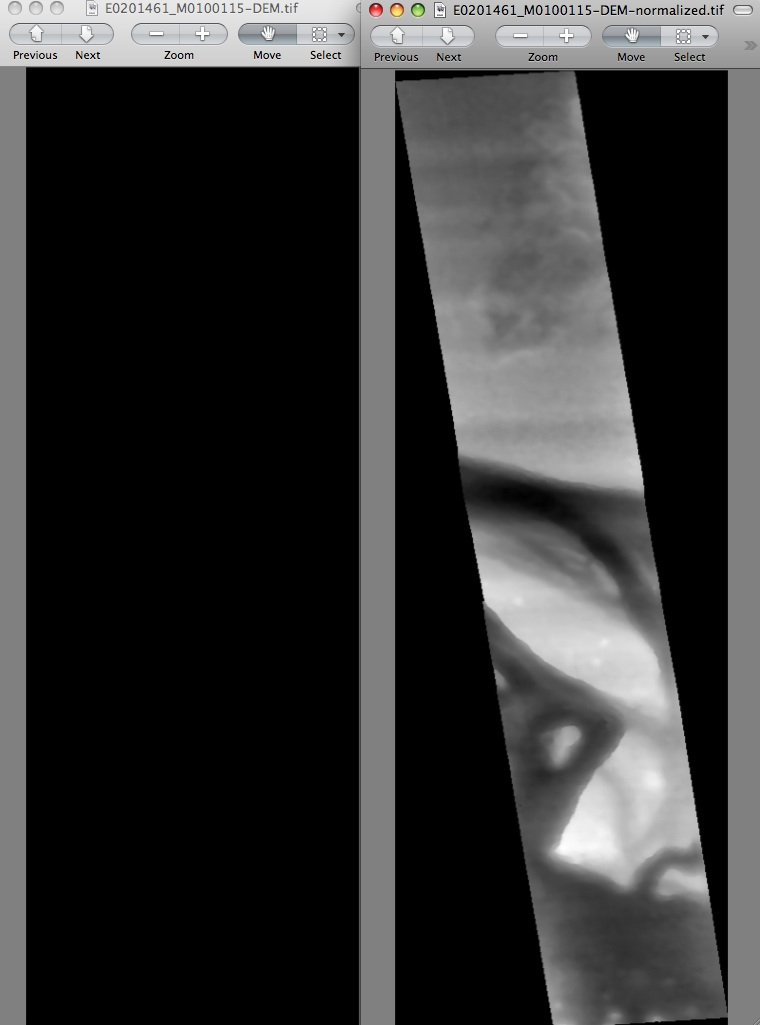
\includegraphics[width=4in]{images/p19-dems.png}
% \caption[P19 dem images]{
%     \label{p19-dems}
% 	The non-normalized and normalized DEMs. Note that the
% 	non-normalized version contains floating point pixel values
% 	and will not open in most image viewing programs which
% 	expect integer pixel values between 0 and 255 (which is
% 	what the normalized version does for you).
%     }
% \end{center}
% \end{figure}
%
% \begin{figure}
% \begin{center}
% \includegraphics[width=3in]{images/p19-ortho.png}
% \caption[P19 orthophoto]{
%     \label{p19-ortho}
% 	The left image orthoprojected onto the DEM.
%     }
% \end{center}
% \end{figure}

Once you have generated a DEM file, you can use the Vision Workbench's
\texttt{colormap} and \texttt{hillshade} tools to create colorized
and/or shaded relief images from the DEM.

To create a colorized version of the DEM, you need only specify the
DEM file to use. Yet alternatively you can specific your own min and
max color ranges.

\begin{verbatim}
    colormap p19-DEM.tif -o p19-colorized.tif
\end{verbatim}

To create a hillshade of the DEM, you should specify the DEM file
to use. It is also advisable to explore the effects of altering the
elevation of the light source.

\begin{verbatim}
    hillshade p19-DEM.tif -o p19-shaded.tif -e 25
\end{verbatim}

To create a colorized version of the shaded relief file, specify
the DEM and the shaded relief file that should be used.

\begin{verbatim}
    colormap p19-DEM.tif --shaded-relief-file p19-shaded.tif -o p19-color-shaded.tif
\end{verbatim}

\begin{figure}
\begin{center}
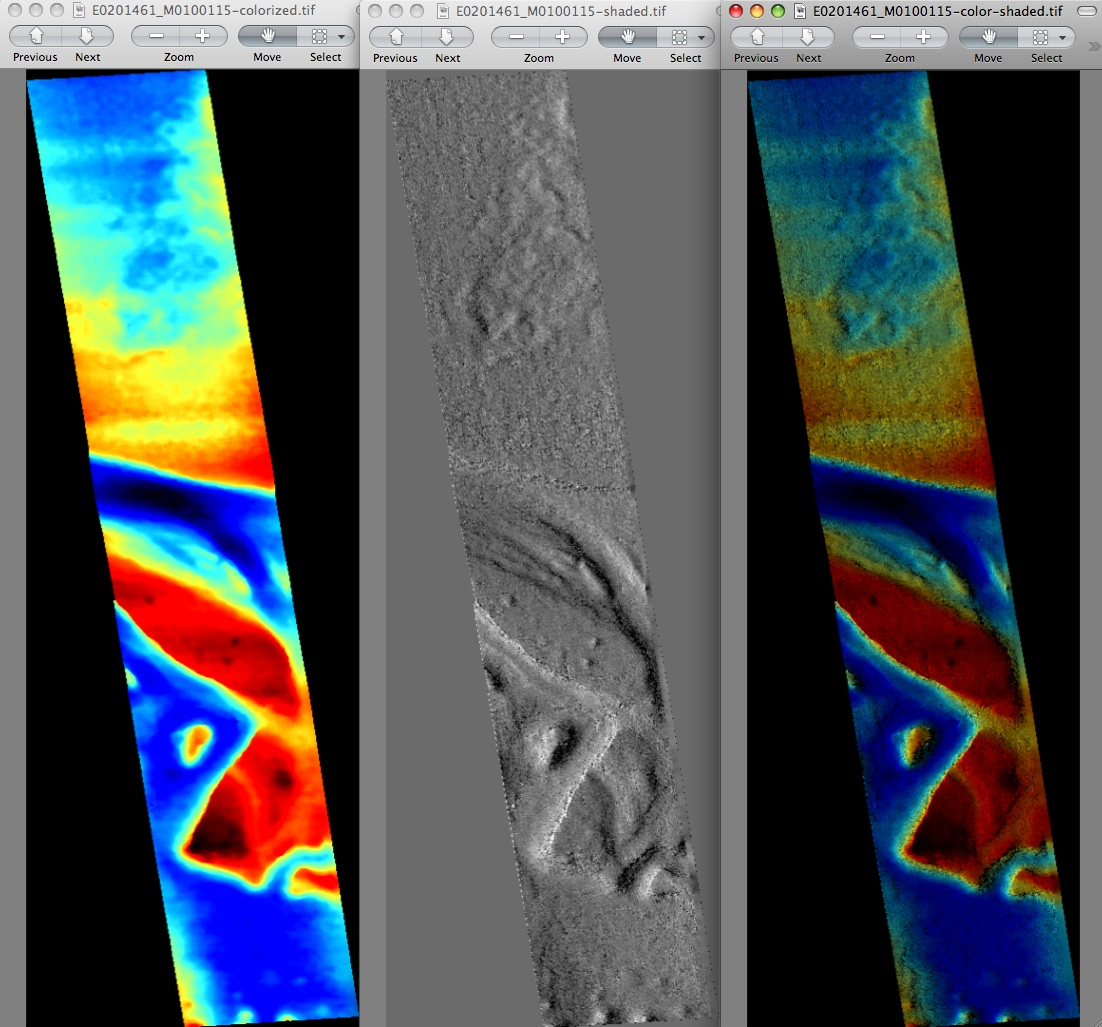
\includegraphics[width=5in]{images/p19-colorized-shaded.png}
\caption[P19 colorized and shaded relief]{
    \label{p19-color}
	The colorized DEM, the shaded relief image, and the colorized hillshade.
    }
\end{center}
\end{figure}

The final option of the stereo processing package is
\texttt{image2qtree}.  This function was designed for use in creating
geographically referenced images in tiles such that each tile can be
viewed at ideal resolution. It can also be used to create KML files
that can be viewed in Google Earth. The program can be used on any of
the following files that you have generated:
\begin{verbatim}
    p19-DEM-normalized.tif
    p19-DRG.tif
    p19-shaded.tif
    p19-colorized.tif
    p19-shaded-colorized.tif
\end{verbatim}

Specify which image you would like to invoke \texttt{image2qtree}
on. Below makes an overlay that can be viewed in Google Mars.

\begin{verbatim}
    image2qtree p19-DEM-normalized.tif -m kml --draw-order 100
\end{verbatim}


%% \section{Preparing Selected Data}

%% There are many ways to process different kinds of image data, and
%% some will be more appropriate for operations by the Stereo Pipeline
%% than others.  While we strive to make the Stereo Pipeline extensible
%% and robust, there are a limited (but growing) set of data that we
%% have thoroughly tested.

%% This section outlines the suggested pre-processing steps to prepare
%% specific data sets for use in the Stereo Pipeline.

%% \subsection{Mars Oribiter Camera (MOC)}

%% MOC images (ending in \texttt{.imq} or \texttt{.img}) can be downloaded from
%% the PDS and only require a single ISIS command to prepare for Stereo Pipeline use:

%% \begin{verbatim}
%%     ISIS 3> mocproc from= MOCimage.imq to= MOCimage.cub Mapping= NO
%% \end{verbatim}

%% The resulting ISIS cube file (e.g. \texttt{MOCimage.cub}) is now ready
%% for processing by the \texttt{stereo} program.


%% \subsection{High Resolution Imaging Science Experiment (HiRISE)}

%% HiRISE images are more complicated.

%% At the moment, the `best' processing method is to start with HiRISE
%% \texttt{*.balance.cub} files (available only internally to the
%% HiRISE team) and run them through the USGS's \texttt{hinoproj.pl}
%% script.  This results in \texttt{noproj}ed and de-jittered cube
%% files that can be run.

%% In the future (who knows when), the HiRISE team will directly produce
%% \texttt{noproj}ed images (dejittered through a different, improved,
%% algorithm) which will be available in the \texttt{extras/} directory
%% of the HiRISE PDS Volume.  And those images will probably be directly
%% usable by the Stereo Pipeline.

%% \emph{As you can tell, I'm still in the process of tracking all of this down. -RAB}


\part{The Stereo Pipeline in Depth}
\chapter{Stereo Correlation}
\label{ch:correlation}

In this chapter we will dive much deeper into understanding the core
algorithms in the Stereo Pipeline.  We start with an overview of the
five stages of stereo reconstruction.  Then we move into an in-depth
discussion and exposition of the various correlation algorithms.

The goal of this chapter is to build an intuition for the stereo
correlation process.  This will help users to identify unusual results
in their \acp{DEM} and hopefully eliminate them by tuning various
parameters in the \texttt{stereo.default} file (appendix
\ref{ch:stereodefault}).  For scientists and
engineers who are using \acp{DEM} produced with the Stereo Pipeline, this
chapter may help to answer the question, ``What is the Stereo Pipeline
doing to the raw data to produce this \ac{DEM}?''

A related question that is commonly asked is, ``How accurate is a \ac{DEM}
produced by the Stereo Pipeline?''  This chapter does not yet address
matters of accuracy and error, however we have several efforts underway
to quantify the accuracy of Stereo Pipeline-derived \acp{DEM}, and will be
publishing more information about that shortly.  Stay tuned.

The entire stereo correlation process, from raw input images to a
point cloud or DEM, can be viewed as a multistage pipeline as depicted
in Figure~\ref{fig:asp}, and detailed in the following sections.

\begin{figure}[tb]
  \centering
  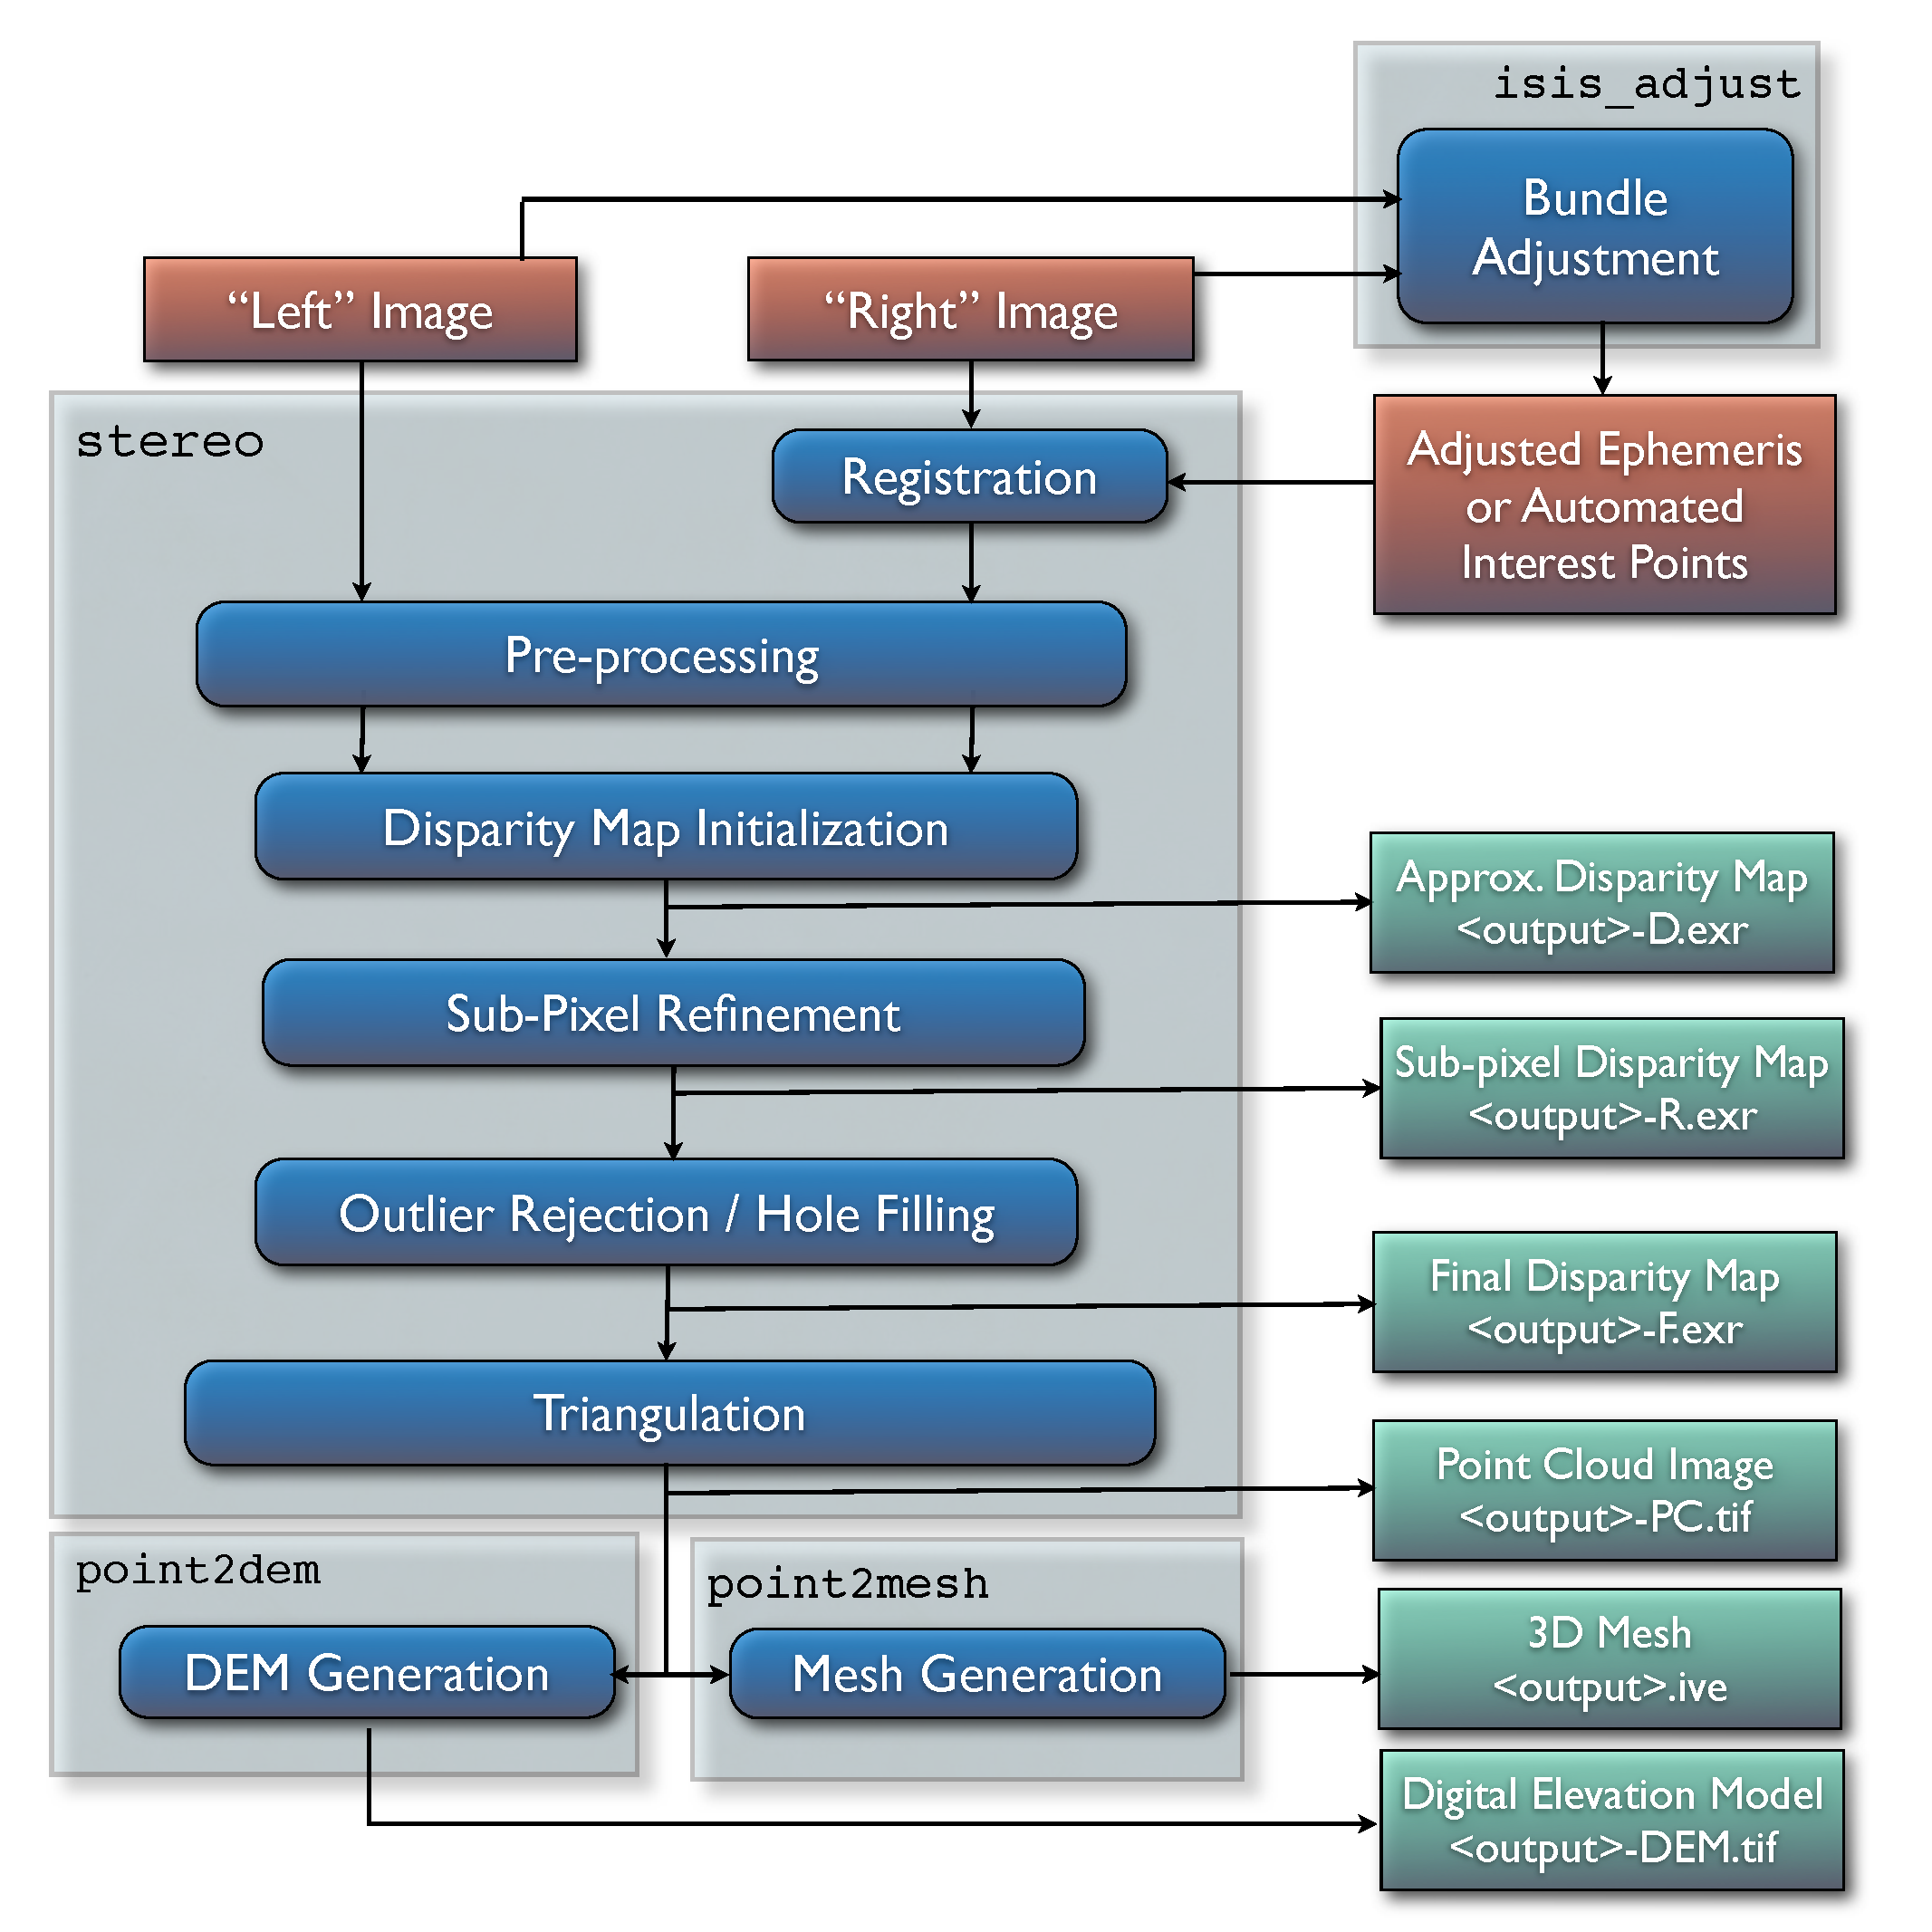
\includegraphics[width=13cm]{images/asp.pdf}
  \caption{Flow of data through the Stereo Pipeline.}
  \label{fig:asp}
\end{figure}

\section{Pre-Processing}

The first optional (but recommended) step in the process is least
squares Bundle Adjustment, which is described in detail in
Chapter~\ref{ch:bundle_adjustment}.

Next, the left and right images are roughly aligned using one of the
four methods: (1) a homography transform of the right image based on
automated tie-point measurements, (2) an affine epipolar transform of
both the left and right images (also based on tie-point measurements as
earlier), the effect of which is equivalent to rotating the original
cameras which took the pictures, (3) a 3D rotation that achieves
epipolar rectification {\it(only implemented for Pinhole sessions for
missions like MER or K10 -- see sections \ref{mer:example} and
\ref{k10:example})} or (4) map-projection of both the left and right
images using the \ac{ISIS} \texttt{cam2map} command or through the more
general \texttt{mapproject} tool that works for any cameras supported by
ASP (see section \ref{mapproj-example} for the latter).  The first three
options can be applied automatically by the Stereo Pipeline when the
\texttt{alignment-method} variable in the \texttt{stereo.default} file
is set to \texttt{affineepipolar}, \texttt{homography}, or
\texttt{epipolar}, respectively.

The latter option, running {\tt cam2map}, {\tt cam2map4stereo.py}, or
{\tt mapproject} must be carried out by the user prior to
invoking the {\tt stereo} command.  Map-projecting the images using
\ac{ISIS} eliminates any unusual distortion in the image due to the
unusual camera acquisition modes (e.g. pitching ``ROTO'' maneuvers
during image acquisition for \ac{MOC}, or highly elliptical orbits and
changing line exposure times for the \acl{HRSC}, \acs{HRSC}).  It also
eliminates some of the perspective differences in the image pair that
are due to large terrain features by taking the existing low-resolution
terrain model into account (e.g., the \acl{MOLA}, \acs{MOLA};
\acl{LOLA}, \acs{LOLA}; \acl {NED}, \acs {NED}; or \acl{ULCN},
\acs{ULCN}, 2005 models).

In essence, map-projecting the images results in a pair of very
closely matched images that are as close to ideal as possible given
existing information. This leaves only small perspective differences
in the images, which are exactly the features that the stereo
correlation process is designed to detect.

For this reason, we recommend map-projection for pre-alignment of most
stereo pairs. Its only cost is longer triangulation times as more math
must be applied to work back through the transforms applied to the images. In
either case, the pre-alignment step is essential for performance
because it ensures that the disparity search space is bounded to a
known area.  In both cases, the effects of pre-alignment are taken
into account later in the process during triangulation, so you do not
need to worry that pre-alignment will compromise the geometric
integrity of your \ac{DEM}.

In some cases the pre-processing step may also normalize the pixel
values in the left and right images to bring them into the same
dynamic range.  Various options in the {\tt stereo.default} file
affect whether or how normalization is carried out, including
\texttt{individually-normalize} and
\texttt{force-use-entire-range}.  Although the defaults work in
most cases, the use of these normalization steps can vary from data
set to data set, so we recommend you refer to the examples in Chapter
\ref{ch:examples} to see if these are necessary in your use case.

Finally, pre-processing can perform some filtering of the input
images (as determined by \\ \texttt{prefilter-mode}) to reduce noise
and extract edges in the images.  When active, these filters apply
a kernel with a sigma of \texttt{prefilter-kernel-width} pixels
that can improve results for noisy images (\texttt{prefilter-mode}
must be chosen carefully in conjunction with \texttt{cost-mode},
see Appendix~\ref{ch:stereodefault}).  The pre-processing modes
that extract image edges are useful for stereo pairs that do not
have the same lighting conditions, contrast, and absolute brightness
\citep{Nishihara84practical}.  We recommend that you use the defaults
for these parameters to start with, and then experiment only if
your results are sub-optimal.

\section{Disparity Map Initialization}
\label{d-sub}

Correlation is the process at the heart of the Stereo Pipeline.  It is
a collection of algorithms that compute correspondences between pixels
in the left image and pixels in the right image.  The map of these
correspondences is called a {\em disparity map}.  You can think of a
disparity map as an image whose pixel locations correspond to
the pixel $(u,v)$ in the left image, and whose pixel values
contain the horizontal and vertical offsets $(d_u, d_v)$ to the
matching pixel in the right image, which is $(u+d_u, v+d_v)$.

The correlation process attempts to find a match for every pixel in
the left image. The only pixels skipped are those marked invalid in
the mask images. For large images (e.g. from \ac{HiRISE}, \acl{LROC},
\acs{LROC}, or WorldView), this is very expensive computationally, so
the correlation process is split into two stages.  The disparity map
initialization step computes approximate correspondences using a
pyramid-based search that is highly optimized for speed, but trades
resolution for speed. The results of disparity map initialization are
integer-valued disparity estimates.  The sub-pixel refinement step
takes these integer estimates as initial conditions for an iterative
optimization and refines them using the algorithm discussed in the
next section.

We employ several optimizations to accelerate disparity map
initialization: (1) a box filter-like accumulator that reduces
duplicate operations during correlation \citep{Sun02rectangular}; (2) a
coarse-to-fine pyramid based approach where disparities are estimated
using low-resolution images, and then successively refined at higher
resolutions; and (3) partitioning of the disparity search space into
rectangular sub-regions with similar values of disparity determined in
the previous lower resolution level of the
pyramid \citep{Sun02rectangular}.

\begin{figure}[bt]
  \centering
  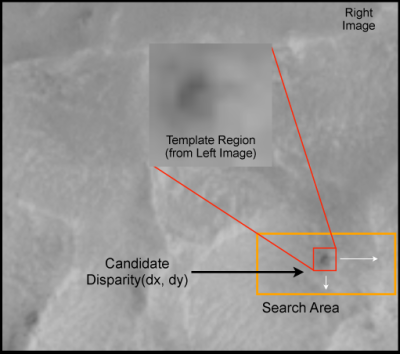
\includegraphics[width=13cm]{images/correlation/correlation_400px.png}
  \caption{The correlation algorithm in disparity map initialization
    uses a sliding template window from the left image to find the
    best match in the right image.  The size of the template window
    can be adjusted using the \texttt{H\_KERN} and \texttt{V\_KERN} parameters in the
    \texttt{stereo.default} file, and the search range can be adjusted
    using the \{\texttt{H},\texttt{V}\}\texttt{\_CORR\_}\{\texttt{MIN}/\texttt{MAX}\} parameters.}
  \label{fig:correlation_window}
\end{figure}

Naive correlation itself is carried out by moving a small, rectangular
template window from the from left image over the specified search
region of the right image, as in Figure~\ref{fig:correlation_window}.
The ``best'' match is determined by applying a cost function that
compares the two windows. The location at which the window evaluates
to the lowest cost compared to all the other search locations is
reported as the disparity value. The \texttt{cost-mode} variable allows you
to choose one of three cost functions, though we recommend normalized
cross correlation \citep{Menard97:robust}, since it is most robust to
slight lighting and contrast variations between a pair of
images. Try the others if you need more speed at the cost of quality.

Our implementation of pyramid correlation is a little unique in that
it is actually split into two levels of pyramid searching. There is a
\texttt{\textit{output\_prefix}-D\_sub.tif} disparity image that is
computed from the greatly reduced input images \texttt{*-L\_sub.tif}
and \texttt{\textit{output\_prefix}-R\_sub.tif}. Those ``sub'' images
have their size chosen so that their area is around 2.25 mega pixels,
a size that is easily viewed on the screen unlike the raw source
imagery. The low-resolution disparity image then defines the per
thread search range of the higher resolution disparity,
\texttt{\textit{output\_prefix}-D.tif}.

This solution is imperfect but comes from our model of multi-threaded
processing. ASP processes individual tiles of the output disparity
in parallel. The smaller the tiles, the easier it is to distribute
evenly among the CPU cores. The size of the tile unfortunately
limits the max number of pyramid levels we can process. We've struck
a balance where every 1024 by 1024 pixel area is processed individually
in a tile. This practice allows only 5 levels of pyramid processing.
With the addition of the second tier of pyramid searching with
\texttt{\textit{output\_prefix}-D\_sub.tif}, we are allowed to
process beyond that limitation.

Any large failure in the low-resolution disparity image will be
detrimental to the performance of the higher resolution disparity. In
the event that the low-resolution disparity is completely unhelpful, it
can be skipped by adding \texttt{corr-seed-mode 0} in the
\texttt{stereo.default} file and using a manual search range (section
\ref{sec:search_range}). This should only be considered in cases where
the texture in an image is completely lost when subsampled. An example
would be satellite imagery of fresh snow in the Arctic. Alternatively,
\texttt{\textit{output\_prefix}-D\_sub.tif} can be computed at a sparse
set of pixels at full resolution, as described in section
\ref{sparse-disp}.

An alternative to computing \texttt{\textit{output\_prefix}-D.tif}
from sub-sampled images (\texttt{corr-seed-mode 1}) or skipping it
altogether (\texttt{corr-seed-mode 0}), is to compute it from a
lower-resolution DEM of the area (\texttt{corr-seed-mode 2}). In this
situation, the low-resolution DEM needs to be specified together with its estimated
error. See section \ref{corr_section} for more detailed information as
to how to specify these options. In our experiments, if the input DEM
has a resolution of 1 km, a good value for the DEM error is about 10 m,
or higher if the terrain is very variable.

\subsection{Debugging Disparity Map Initialization}

Never will all pixels be successfully matched during stereo
matching. Though a good chunk of the image should be correctly
processed. If you see large areas where matching failed, this could be
due to a variety of reasons:

\begin{itemize}
\item In regions where the images do not overlap, there should be no
  valid matches in the disparity map.
\item Match quality may be poor in regions of the images that have
  different lighting conditions, contrast, or specular properties of
  the surface.
\item Areas that have image content with very little texture or
  extremely low contrast may have an insufficient signal to noise
  ratio, and will be rejected by the correlator.
\item Areas that are highly distorted due to different image
  perspective, such as crater and canyon walls, may exhibit poor
  matching performance. This could also be due to failure of the
  preprocessing step in aligning the images. The correlator can not
  match images that are rotated differently from each other or have
  different scale/resolution. Mapprojection is used to at least
  partially rectifly these issues (section \ref{mapproj-example}).
\end{itemize}

Bad matches, often called ``blunders'' or ``artifacts'' are also
common, and can happen for many of the same reasons listed above.  The
Stereo Pipeline does its best to automatically detect and eliminate
these blunders, but the effectiveness of these outlier rejection
strategies does vary depending on the quality of the input imagery.

When tuning up your {\tt stereo.default} file, you will find that
it is very helpful to look at the raw output of the disparity map
initialization step.  This can be done using the {\tt disparitydebug}
tool, which converts the \texttt{\textit{output\_prefix}-D.tif}
file into a pair of normal images that contain the horizontal and
vertical components of disparity.  You can open these in a standard
image viewing application and see immediately which pixels were
matched successfully, and which were not. Stereo matching blunders
are usually also obvious when inspecting these images.  With a good
intuition for the effects of various {\tt stereo.default} parameters
and a good intuition for reading the output of {\tt disparitydebug},
it is possible to quickly identify and address most problems.

If you are seeing too many holes in your disparity images, one option 
that may give good results is to increase the size of the
correlation kernel used by \texttt{stereo\_corr} with the 
\texttt{--corr-kernel} option.  Increasing the kernel size will 
increase the processing time but should help fill in regions of
the image where no match was found.  

\begin{figure}[tb]
  \centering
  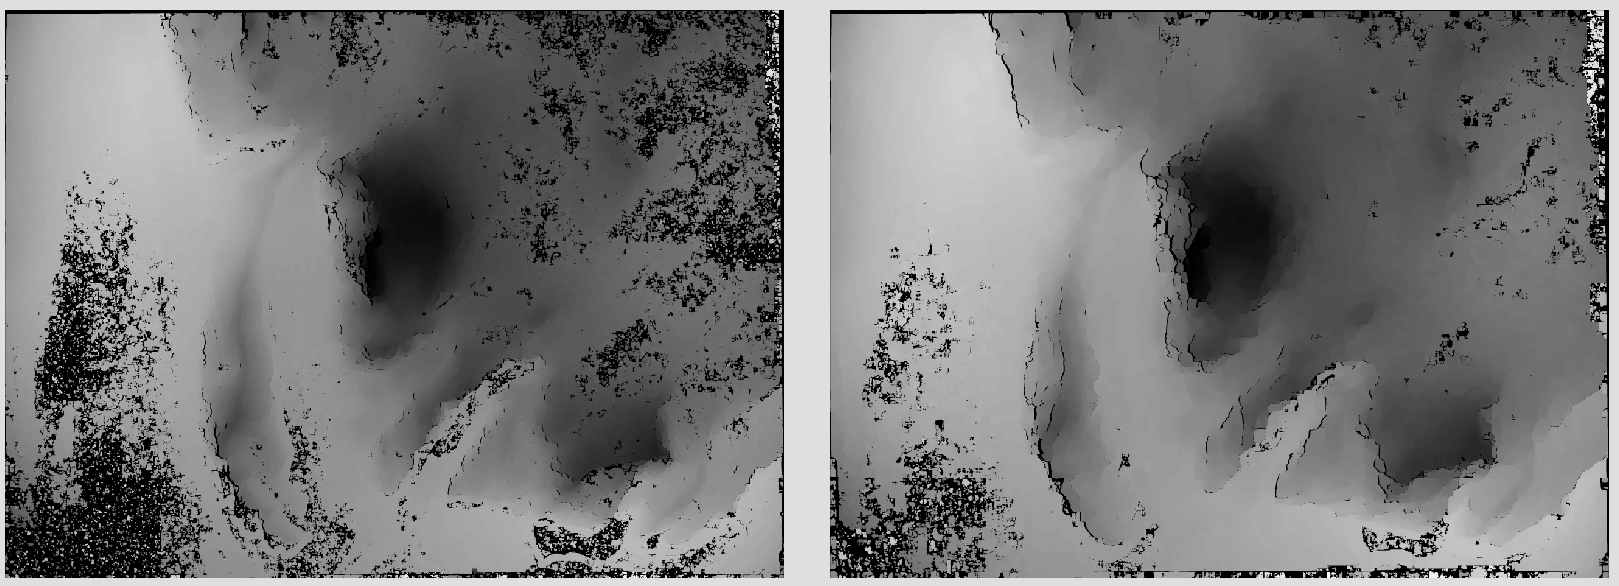
\includegraphics[width=17cm]{images/correlation/stereo_corr_box_compare.png}
  \caption{The effect of increasing the correlation kernel size from 35 (left) 
  to 75 (right). This location is covered in snow and several regions lack 
  texture for the correlator to use but a large kernel increases the chances 
  of finding useful texture for a given pixel.}
  \label{fig:corr-kernel-size-effect}
\end{figure}


\begin{figure}[tb]
  \centering
  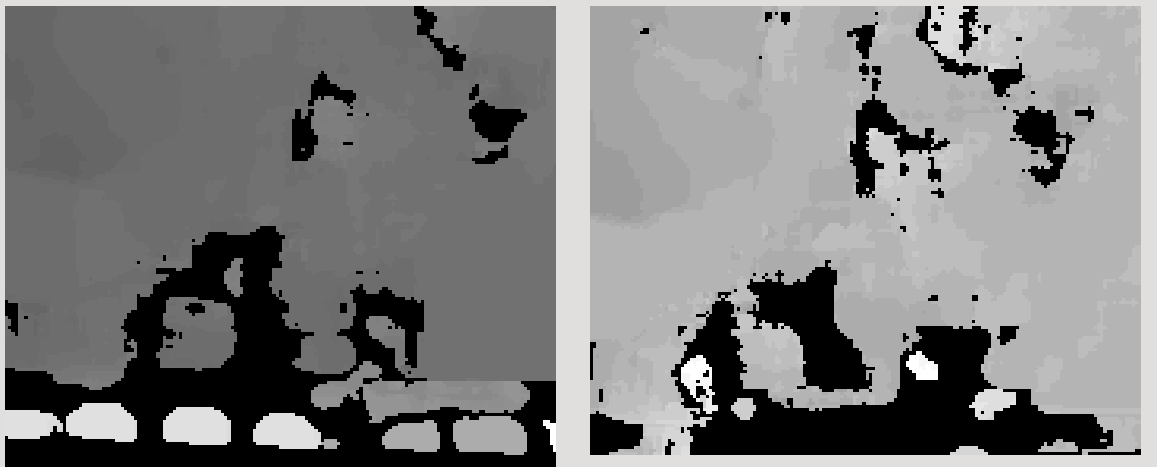
\includegraphics[width=17cm]{images/correlation/quantile_filter_result.png}
  \caption{The effect of using the \texttt{rm-quantile} filtering option
  in \texttt{stereo\_corr}. In the left image there are a series of high
  disparity "islands" at the bottom of the image.  In the right image quantile
  filtering has removed those islands while leaving the rest of the image intact.}
  \label{fig:quantile-filtering-effect}
\end{figure}


\subsection{Search Range Determination}
\label{sec:search_range}

In some circumstances, the low-resolution
disparity \texttt{D\_sub.tif} may fail to get computed, or it may be
inaccurate. This can happen for example if only very small features are
present in the original images, and they disappear during the resampling
that is necessary to obtain \texttt{D\_sub.tif}. In this case, it is
possible to set \texttt{corr-seed-mode} to 0, and manually set a search
range to use for full-resolution correlation via the parameter
\texttt{corr-search}. In \texttt{stereo.default} this parameter's entry
will look like:

\begin{verbatim}
        corr-search -80 -2 20 2
\end{verbatim}

The exact values to use with this option you'll have to discover
yourself. The numbers right of \texttt{corr-search} represent the
horizontal minimum boundary, vertical minimum boundary, horizontal
maximum boundary, and finally the horizontal maximum boundary within
which we will search for the disparity during correlation.

It can be tricky to select a good search range for the \texttt{stereo.default} file.
That's why the best way is to let \texttt{stereo} perform an automated
guess for the search range. If you find that you can do a
better estimate of the search range, take look at the intermediate
disparity images using the \texttt{disparitydebug} program to figure
out which search directions can be expanded or contracted. The output
images will clearly show good data or bad data depending on whether
the search range is correct.

The worst case scenario is to determine the search range manually. For
example, for ISIS images, both images could be opened in \texttt{qview}
and the coordinates of points that can be matched visually can be
compared. Subtract line,sample locations in the first image from the
coordinates of the same feature in the second image, and this will yield
offsets that can be used in the search range.  Make several of these
offset measurements and use them to define a line,sample bounding box,
then expand this by 50\% and use it for \texttt{corr-search}.  This will
produce good results in most images.

Also, if you are using an alignment option, you'll instead want to
make those disparity measurements against the written L.tif and R.tif
files (see chapter \ref{chapter:outputfiles}) instead of the original input files.

\subsection{Local Homography}
\label{sec:local_hom}

Correlation works by decomposing the left image into tiles, and for each
pixel in each tile finding the best-matching pixel in the right image.

Depending on user's choices, by this stage either the left or the right
image (or both) may already be transformed so that they are very
similar, making the matching process more likely to succeed.

Whether that is the case or not, Stereo Pipeline can estimate, based on
the low-resolution disparity
\texttt{\textit{output\_prefix}-D\_sub.tif}, a local homography transform
for every left image tile, which, when applied to the right image,
improves the similarity of the right image to the current left image tile. This
option can be turned on with the flag \texttt{use-local-homography}.

This local homography transform comes in most useful when a global
homography transform could not be applied (for example, if interest
point matching failed). The input low-resolution disparity can be
computed in several ways, as described earlier in the section.


\section{Sub-pixel Refinement}
\label{sec:subpixel}

Once disparity map initialization is complete, every pixel in the
disparity map will either have an estimated disparity value, or it
will be marked as invalid.  All valid pixels are then adjusted in the
sub-pixel refinement stage based on the \texttt{subpixel-mode}
setting. % Subpixel refinement is not additive step.

The first mode is parabola-fitting sub-pixel refinement
(\texttt{subpixel-mode 1}).  This technique fits a 2D parabola to
points on the correlation cost surface in an 8-connected neighborhood
around the cost value that was the ``best'' as measured during
disparity map initialization. The parabola's minimum can then be
computed analytically and taken as as the new sub-pixel disparity
value.

This method is easy to implement and extremely fast to compute, but it
exhibits a problem known as pixel-locking: the sub-pixel disparities
tend toward their integer estimates and can create noticeable ``stair
steps'' on surfaces that should be smooth
\citep{Stein06:attenuating,Szeliski03sampling}.  See
for example Figure~\ref{fig:parabola_subpixel}. Furthermore, the parabola
subpixel mode is not capable of refining a disparity estimate by more
than one pixel, so although it produces smooth disparity maps, these
results are not much more accurate than the results that come out of
the disparity map initialization in the first place.  However, the
speed of this method makes it very useful as a ``draft'' mode for
quickly generating a \ac{DEM} for visualization (i.e. non-scientific)
purposes. It is also beneficial in the event that a user will simply
downsample their DEM after generation in Stereo Pipeline.

\begin{figure}[tb]
\centering
  \subfigure[{\tt Left Image}]{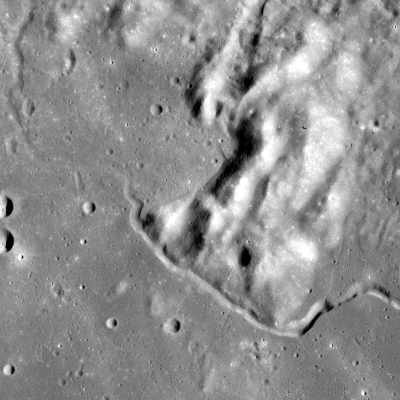
\includegraphics[width=2in]{images/correlation/sub4-AS15-M-1134_crop_400px.png}
    \label{fig:left_input_image}}
  \subfigure[{\tt Parabola Subpixel Mode}]{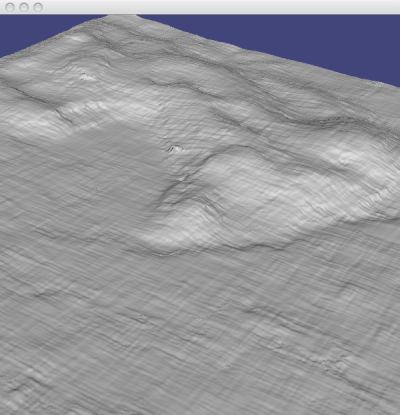
\includegraphics[width=2in]{images/correlation/3D_mode0_400px.png}
    \label{fig:parabola_subpixel}}
  \subfigure[{\tt Bayes EM Subpixel Mode}]{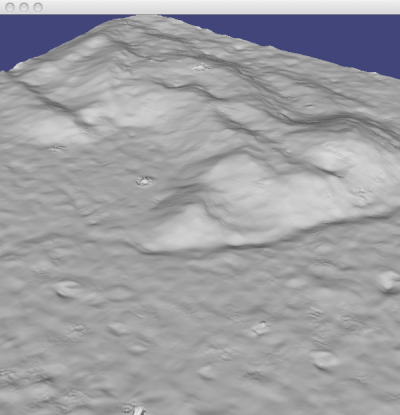
\includegraphics[width=2in]{images/correlation/3D_mode3_400px.png}}

  \subfigure[{\tt Right Image}]{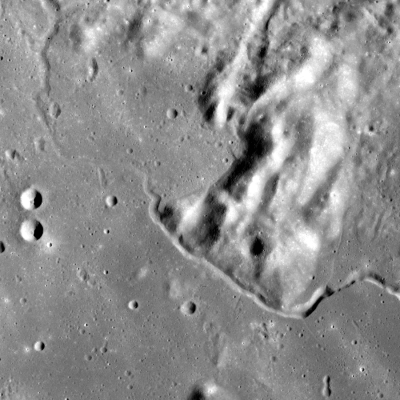
\includegraphics[width=2in]{images/correlation/sub4-AS15-M-1135_crop_400px.png}
    \label{fig:right_input_image}}
  \subfigure[{\tt Parabola Hillshade}]{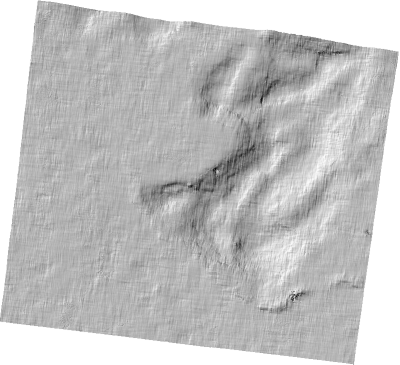
\includegraphics[width=2in]{images/correlation/hillshade_mode0_400px.png}}
  \subfigure[{\tt Bayes EM Hillshade}]{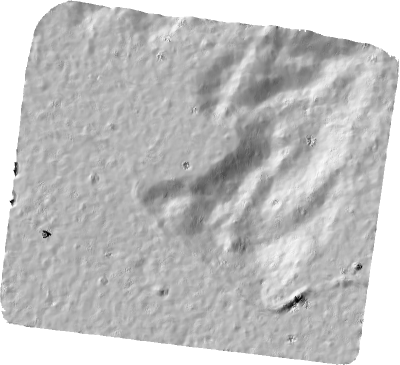
\includegraphics[width=2in]{images/correlation/hillshade_mode3_400px.png}}

\caption{Left: Input images.  Center: results using the parabola draft
  subpixel mode (\texttt{subpixel-mode = 1}). Right: results using the Bayes
  EM high quality subpixel mode (\texttt{subpixel-mode = 2}).}
\label{fig:parabola_results}
\end{figure}

For high quality results, we recommend \texttt{subpixel-mode 2}:
the Bayes EM weighted affine adaptive window correlator.  This
advanced method produces extremely high quality stereo matches that
exhibit a high degree of immunity to image noise.  For example
Apollo Metric Camera images are affected by two types of noise
inherent to the scanning process: (1) the presence of film grain
and (2) dust and lint particles present on the film or scanner.
The former gives rise to noise in the \ac{DEM} values that wash out real
features, and the latter causes incorrect matches or hard to detect
blemishes in the \ac{DEM}.  Attenuating the effect of these scanning
artifacts while simultaneously refining the integer disparity map
to sub-pixel accuracy has become a critical goal of our system, and
is necessary for processing real-world data sets such as the Apollo
Metric Camera data.

The Bayes EM subpixel correlator also features a deformable template
window from the left image that can be rotated, scaled, and translated
as it zeros in on the correct match in the right image.  This
adaptive window is essential for computing accurate matches on crater
or canyon walls, and on other areas with significant perspective
distortion due to foreshortening.

This affine-adaptive behavior is based on the Lucas-Kanade template
tracking algorithm, a classic algorithm in the field of computer
vision \citep{Baker04:lucas-kanade}.  We have extended this technique;
developing a Bayesian model that treats the Lucas-Kanade parameters
as random variables in an Expectation Maximization (EM) framework.
This statistical model also includes a Gaussian mixture component
to model image noise that is the basis for the robustness of our
algorithm.  We will not go into depth on our approach here, but we
encourage interested readers to read our papers on the topic
\citep{nefian:bayes_em, broxton:isvc09}.

However we do note that, like the computations in the disparity map
initialization stage, we adopt a multi-scale approach for sub-pixel
refinement. At each level of the pyramid, the algorithm is initialized
with the disparity determined in the previous lower resolution level
of the pyramid, thereby allowing the subpixel algorithm to shift the
results of the disparity initialization stage by many pixels if a better
match can be found using the affine, noise-adapted window.  Hence,
this sub-pixel algorithm is able to significantly improve upon the
results to yield a high quality, high resolution result.

Another option when run time is important is \texttt{subpixel-mode 3}:
the simple affine correlator.  This is essentially the Bayes EM mode
with the noise correction features removed in order to decrease the
required run time.  In data sets with little noise this mode can yield
results similar to Bayes EM mode in approximately one fifth the time.

\section{Triangulation}

When running an ISIS session, the Stereo Pipeline uses geometric
camera models available in \ac{ISIS} \citep{anderson08:isis}.  These
highly accurate models are customized for each instrument that
\ac{ISIS} supports.  Each \ac{ISIS} ``cube'' file contains all of the
information that is required by the Stereo Pipeline to find and use
the appropriate camera model for that observation.

Other sessions such as DG (\textit{Digital Globe}) or Pinhole, require that
their camera model be provided as additional arguments to the
\texttt{stereo} command. Those camera models come in the form of an
XML document for DG and as \texttt{*.pinhole, *.tsai, *.cahv,
  *.cahvor} for Pinhole sessions. Those files must be the third and
forth arguments or immediately follow after the 2 input images for
\texttt{stereo}.

\begin{figure}[h]
\centering
  \subfigure[{\tt Framing Camera Model}]{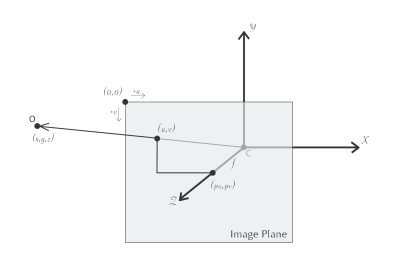
\includegraphics[width=3in]{images/correlation/pinhole_model_400px.png}
    \label{fig:framing}}
  \subfigure[{\tt Pushbroom Camera Model}]{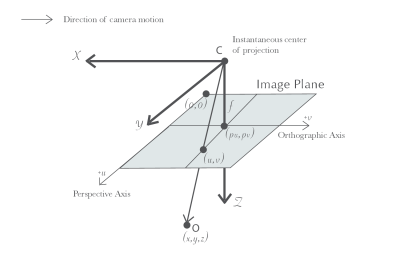
\includegraphics[width=3in]{images/correlation/linescan_model_400px.png}
\label{fig:linescan}}
\caption{Most remote sensing cameras fall into two generic categories
  based on their basic geometry.  Framing cameras (left) capture an
  instantaneous two-dimensional image.  Linescan cameras (right)
  capture images one scan line at a time, building up an image over
  the course of several seconds as the satellite moves through the
  sky.}
\label{fig:camera_models}
\end{figure}

\ac{ISIS} camera models account for all aspects of camera geometry,
including both intrinsic (i.e. focal length, pixel size, and lens
distortion) and extrinsic (e.g. camera position and orientation)
camera parameters.  Taken together, these parameters are sufficient to
``forward project'' a 3D point in the world onto the image plane of
the sensor.  It is also possible to ``back project'' from the camera's
center of projection through a pixel corresponding to the original 3D
point.

\begin{figure}[tb]
  \centering
  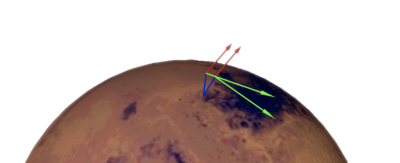
\includegraphics[width=12cm]{images/correlation/triangulation_400px.png}
  \caption{Once a disparity map has been generated and refined, it can
    be used in combination with the geometric camera models to compute
    the locations of 3D points on the surface of Mars.  This figure
    shows the position (at the origins of the red, green, and blue vectors) and
	orientation of the Mars Global Surveyor at
    two points in time where it captured images in a stereo pair.}
  \label{fig:triangulation}
\end{figure}

Notice, however, that forward and back projection are not symmetric
operations.  One camera is sufficient to ``image'' a 3D point onto a
pixel located on the image plane, but the reverse is not true.  Given
only a single camera and a pixel location $x = (u,v),$ that is the
image of an unknown 3D point $P = (x,y,z)$, it is only possible to
determine that $P$ lies somewhere along a ray that emanates from the
camera's center of projection through the pixel location $x$ on the
image plane (see Figure~\ref{fig:camera_models}).

Alas, once images are captured, the route from image pixel back to 3D
points in the real world is through back projection, so we must bring
more information to bear on the problem of uniquely reconstructing our
3D point.  In order to determine $P$ using back projection, we need
{\em two} cameras that both contain pixel locations $x_1$ and $x_2$
where $P$ was imaged.  Now, we have two rays that converge on a point
in 3D space (see Figure~\ref{fig:triangulation}). The location where
they meet must be the original location of $P$.

In practice, the two rays rarely intersect perfectly because any
slight error in the camera position or pointing information will
effect the rays' positions as well.  Instead, we take the {\em closest
  point of intersection} of the two rays as the location of point
$P$.

Additionally, the actual distance between the rays at this point is an
interesting and important error metric that measures how
self-consistent our two camera models are for this point.  You will
learn in the next chapter that this information, when computed and
averaged over all reconstructed 3D points, can be a valuable statistic
for determining whether to carry out bundle adjustment. Distance
between the two rays at their closest intersection is recorded in the
fourth channel of the point cloud file,
\texttt{\textit{output-prefix}-PC.tif}. This information can be
brought to the same perspective as the output DEM by using the
\textit{-\/-error} argument on the \texttt{point2dem} command.

This error in the triangulation, the distance between two rays,
\emph{is not the true accuracy of the DEM}. It is only another
indirect measure of quality. A DEM with high triangulation error
is always bad and should have its images bundle-adjusted. A DEM
with low triangulation error is at least self consistent but could
still be bad. A map of the triangulation error should only be
interpreted as a relative measurement. Where small areas are found
with high triangulation error came from correlation mistakes and
large areas of error came from camera model inadequacies.

\chapter{Bundle Adjustment}
\label{ch:bundle_adjustment}

\newenvironment{myindentpar}[1]
               {\begin{list}{}
                   {\setlength{\leftmargin}{#1}}
                 \item[]
               }
               {\end{list}}

\definecolor{lgray}{gray}{0.95}

Satellite position and orientation errors have a direct effect on the
accuracy of digital elevation models produced by the Stereo Pipeline.
If they're not corrected, these uncertainties will result in
systematic errors in the overall position and slope of the \ac{DEM}.
Severe distortions can occur as well, resulting in twisted or ``taco
shaped'' \acp{DEM}, though in most cases these effects are quite
subtle and hard to detect. In the worse case, such as with old mission
data like Voyager or Apollo, these gross camera misalignments can
prohibit Stereo Pipeline's internal interest point matcher and block
auto search range detection.

USGS's \ac{ISIS} software contains a suite of tools for correcting camera
position and orientation errors for their cameras using a process
called \emph{bundle adjustment}. Bundle adjustment is the process of
simultaneously adjusting the properties of many cameras and the 3D
locations of the objects they see in order to minimize the error
between the estimated, back-projected pixel location of the 3D objects
and their actual measured location in the captured images.

That complex process can be boiled down to this simple idea: bundle
adjustment ensures that observations in multiple different images of a
single ground feature are self-consistent. If they are not consistent,
then the position and orientation of the cameras as well as the 3D
position of the feature must be adjusted until they are.  This
optimization is carried out along with thousands (or more) of similar
constraints involving many different features observed in other
images.  Bundle adjustment is very powerful and versatile: it can
operate on just two overlapping images, or on thousands. It is also a
dangerous tool. Careful consideration is required to insure and
verify that the solution does represent reality.

\begin{figure}[bt]
  \centering
  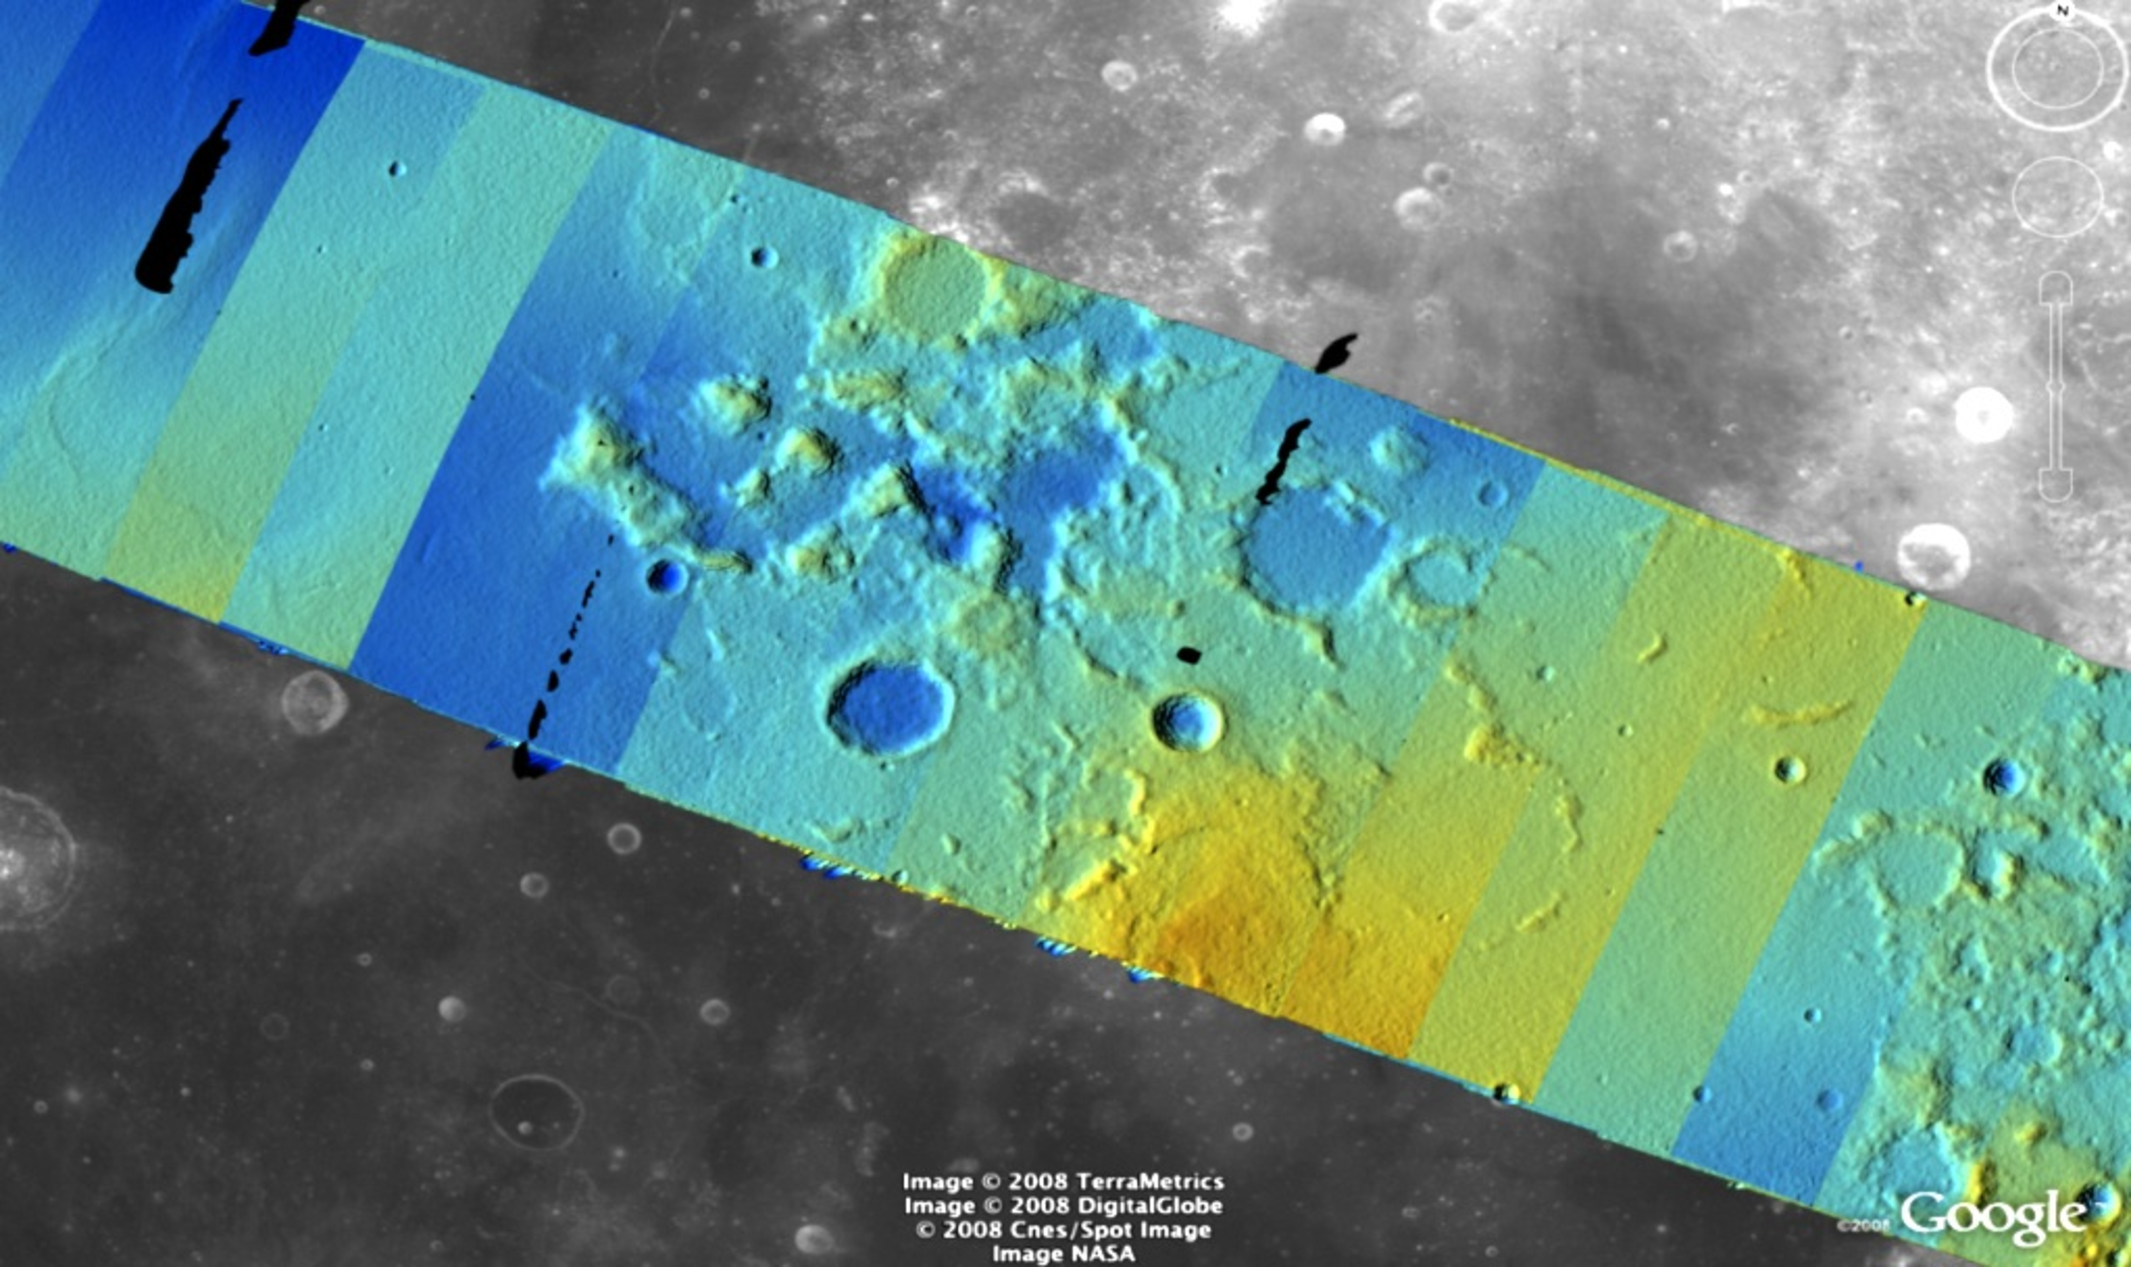
\includegraphics[width=8cm]{images/ba_orig}
  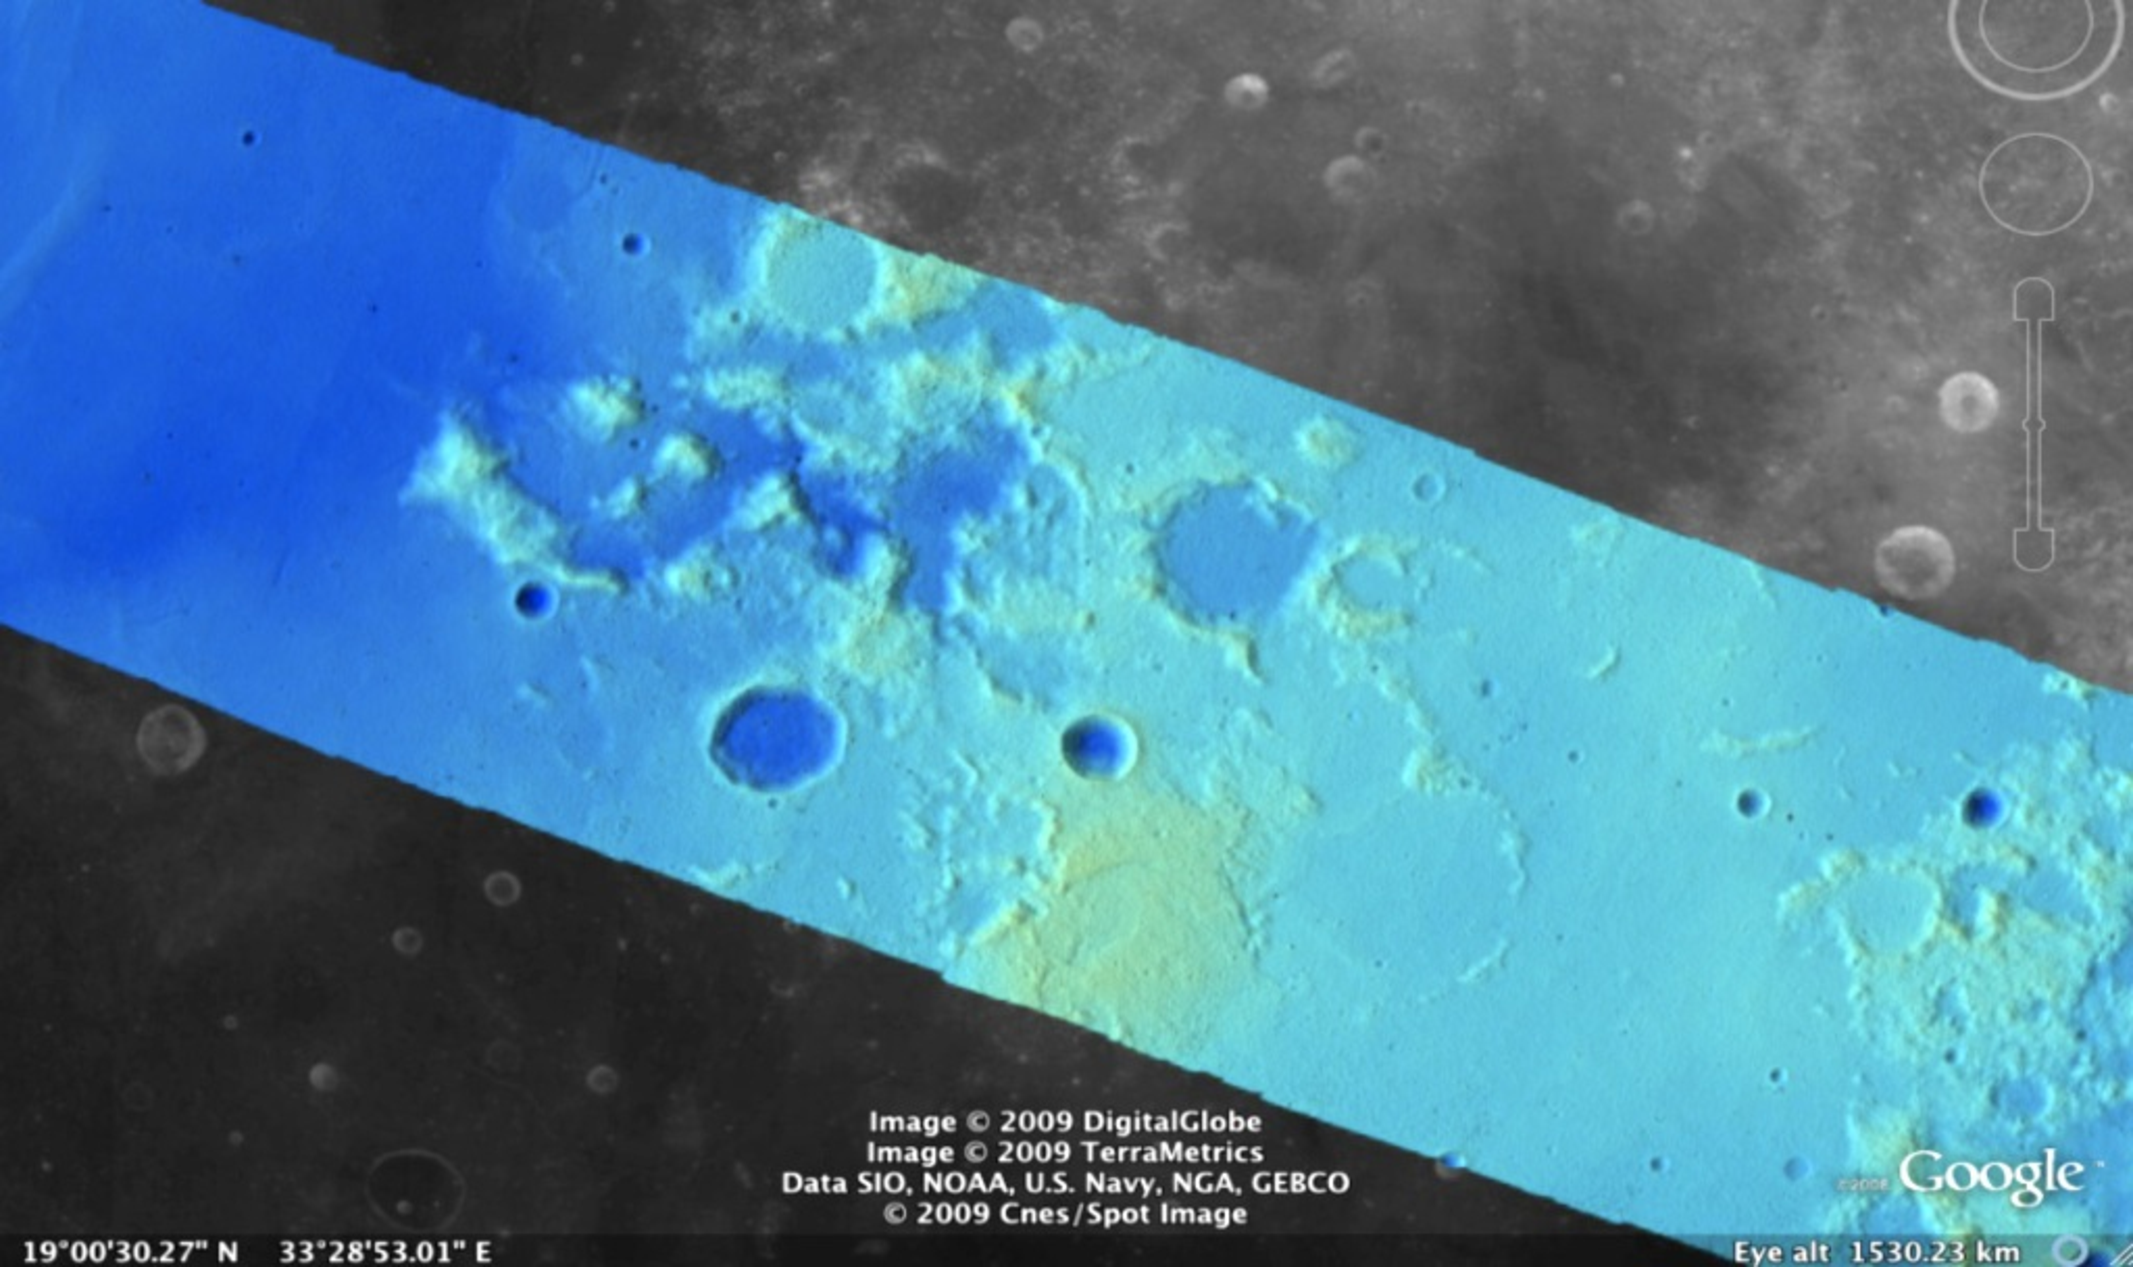
\includegraphics[width=8cm]{images/ba_adjusted}
  \caption{Bundle adjustment is illustrated here using a color-mapped,
    hill-shaded DEM mosaic from Apollo 15, Orbit 33, imagery. (a)
    Prior to bundle adjustment, large discontinuities can exist between
    overlapping DEMs made from different images. (b) After bundle
    adjustment, DEM alignment errors are minimized, and no longer visible.}
  \label{fig:bundle_adjustment}
\end{figure}

Bundle adjustment can also take advantage of \acp{GCP}, which are
3D locations of features that are known apriori (often by measuring
them by hand in another existing \ac{DEM}). \acp{GCP} can improve the internal
consistency of your \ac{DEM} or align your \ac{DEM} to an existing data
product. Finally, even though bundle adjustment calculates the
locations of the 3D objects it views, only the final properties of
the cameras are recorded for use by the Ames Stereo Pipeline. Those
properties can be loaded into the \texttt{stereo} program which
uses its own method for triangulating 3D feature locations.

When using the Stereo Pipeline, bundle adjustment is an optional step
between the capture of images and the creation of \acp{DEM}. The bundle
adjustment process described below should be completed prior to
running the \texttt{stereo} command.

Although bundle adjustment is not a required step for generating
\acp{DEM}, it is {\em highly recommended} for users who plan to
create \acp{DEM} for scientific analysis and publication.  Incorporating
bundle adjustment into the stereo work flow not only results in
\acp{DEM} that are more internally consistent, it is also the correct
way to co-register your \acp{DEM} with other existing data sets and
geodetic control networks.

At the moment however, Bundle Adjustment does not automatically work
against outside DEMs from sources such as laser altimeters. Hand
picked \acp{GCP} are the only way for \ac{ASP} to register to those
types of sources.

\subsection{A deeper understanding}

In bundle adjustment the position and orientation of each camera
station are determined jointly with the 3D position of a set of image
tie-points points chosen in the overlapping regions between
images. Tie points, like they sound, tie individual camera images
together. Their physical manifestation would be a rock or small crater
than can be observed across multiple images.

Tie-points can be automatically extracted using Vision Workbench's
Interest Point module, \ac{ISIS}'s \texttt{autoseed} and \texttt{pointreg},
or through a number of outside methods such as the famous
SURF\citep{surf08}. We'll be discussing the method of gathering these
measurements using \ac{ISIS}'s toolchain. Creating a collection of tie
points, {\it called a control network}, is a three step process. First, a
general geographic layout of the points must be decided upon. This is
traditionally just a grid layout that has some spacing that allows for
about a 20-30 measurements to be made per image. This decided upon grid
shows up in slightly different projected locations each image due to
their slight misalignments. The second step is have an automatic
registration algorithm try to find the same feature in all images using
the prior grid as a starting location. The third step is to manually
verify all measurements visually, checking to insure that each
measurement is looking at the same feature.

\begin{figure}[b!]
  \begin{center}
  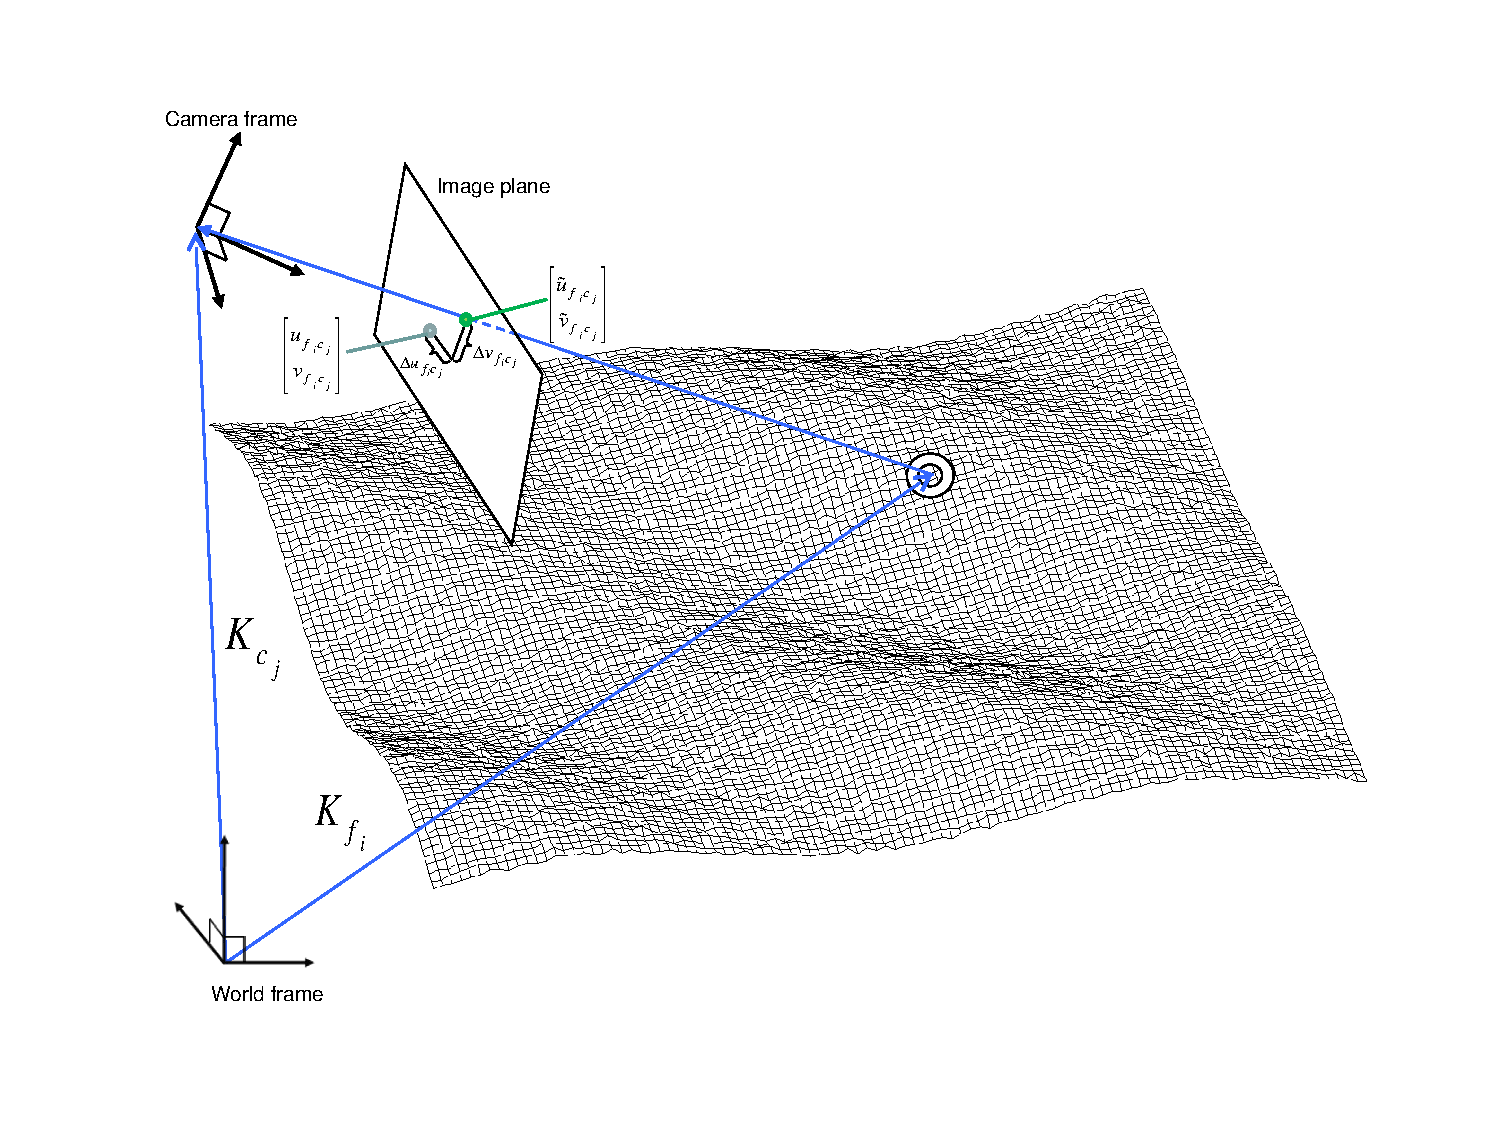
\includegraphics[trim=20mm 20mm 20mm 15mm,clip,width=6in]{images/ba_feature_observation.pdf}
  \end{center}
  \caption{ A feature observation in bundle adjustment, from \citet{moore09} }
  \label{fig:ba_feature}
\end{figure}

Bundle Adjustment in \ac{ISIS} is performed with the \texttt{jigsaw}
executable. It generally follows the method described
in~\cite{triggs00} and determines the best camera parameters that
minimize the projection error given by ${\bf \epsilon} =
\sum_k\sum_j(I_k-I(C_j, X_k))^2$ where $I_k$ are the tie points on the
image plane, $C_j$ are the camera parameters, and $X_k$ are the 3D
positions associated with features $I_k$. $I(C_j, X_k)$ is an image
formation model (i.e. forward projection) for a given camera and 3D
point. To recap, it projects the 3D point, $X_k$, into the camera with
parameters $C_j$. This produces a predicted image location for the 3D
point that is compared against the observed location, $I_k$. It then
reduces this error with the Levenberg-Marquardt algorithm (LMA). Speed
is improved by using sparse methods as described in \citet{hartley04},
\citet{konolige:sparsesparse}, and \citet{cholmod}.

Even though the arithmetic for bundle adjustment sounds clever, there
are faults with the base implementation. Imagine a case where all
cameras and 3D points were collapsed into a single point. If you
evaluate the above cost function, you'll find that the error is indeed
zero. This is not the correct solution if the images were taken
from orbit. Another example is if a translation was applied equally to
all 3D points and camera locations. This again would not affect the
cost function. This fault comes from bundle adjustment's inability to
control the scale and translation of the solution. It will correct the
geometric shape of the problem, yet it cannot guarantee that the solution
will have correct scale and translation.

\ac{ISIS} attempts to fix this problem by adding two additional cost
functions to bundle adjustment. First of which is ${\bf \epsilon} =
\sum_j(C_j^{initial}-C_j)^2$. This constrains camera parameters to
stay relatively close to their initial values. Second, a small handful
of 3D ground control points can be chosen by hand and added to the
error metric as ${\bf \epsilon} = \sum_k(X_k^{gcp}-X_k)^2$ to
constrain these points to known locations in the planetary coordinate
frame. A physical example of a ground control point could be the
location of a lander that has a well known location. GCP could also be
hand picked points against a highly regarded and prior existing map
such as the THEMIS Global Mosaic or the LRO-WAC Global Mosaic.

Like other iterative optimization methods, there are several
conditions that will cause bundle adjustment to terminate. When
updates to parameters become insignificantly small or when the error,
${\bf \epsilon}$, becomes insignificantly small, then the algorithm
has converged and the result is most likely as good as it will get.
However, the algorithm will also terminate when the number of
iterations becomes too large, in which case bundle adjustment may or
may not have finished refining the parameters of the cameras.

\section{Performing bundle adjustment with USGS's ISIS}

Ames Stereo Pipeline at one point provided its own bundle adjustment
utilities but at this point it is of our opinion that they not be used
for general use. USGS's \ac{ISIS} bundle adjustment software has
improved and gets more regular service than we could hope to provide.

This tutorial for ISIS's bundle adjustment tools is taken from
\cite{lunokhod:controlnetwork} and \cite{lunokhod:gcp}. These tools
are not a product of NASA nor the authors of Stereo Pipeline. They
were created by USGS and their documentation is available at
\cite{isis:documentation}.

\subsection{Processing Mars Orbital Camera Imagery} 
\label{sec:ba_example}

What follows is an example of bundle adjustment using two \ac{MOC}
images of Hrad Vallis. We use images E02/01461 and M01/00115, the same
as used in Chapter~\ref{ch:tutorial}. These images are available from
NASA's \ac{PDS} (the \ac{ISIS} \texttt{mocproc} program will operate
on either the IMQ or IMG format files, we use the \texttt{.imq} below
in the example).  For reference, the following \ac{ISIS} commands are
how to convert the \ac{MOC} images to \ac{ISIS} cubes.

\begin{verbatim}
  ISIS 3> mocproc from= e0201461.imq to= e0201461.cub mapping=no
  ISIS 3> mocproc from= m0100115.imq to= m0100115.cub mapping=no
\end{verbatim}

Note that the resulting images are not map projected. Bundle
adjustment requires the ability to project arbitrary 3D points into
the camera frame. The process of map projecting an image dissociates
the camera model from the image. Map projecting can be perceived as
the generation of a new infinitely large camera sensor that may be
parallel to the surface, a conic shape, or something more
complex. That makes it extremely hard to project a random point into
the camera's original model. The math would follow the transformation
from projection into the camera frame, then projected back down to
surface that ISIS uses, then finally up into the infinitely large
sensor. \texttt{Jigsaw} does not support this and thus does not
operate on map projected imagery.

Before we can dive into creating our tie-point measurements we must
finish prepping these images. The following commands will add a vector
layer to the cube file that describes its outline on the globe. It
will also create a data file that describes the overlapping sections
between files.

\begin{verbatim}
  ISIS 3> footprintinit from= e0201461.cub
  ISIS 3> footprintinit from= m0100115.cub
  ISIS 3> echo *cub |  xargs -n1 echo > cube.lis
  ISIS 3> findimageoverlaps from=cube.lis overlaplist=overlap.lis
\end{verbatim}

At this point, we are ready to start generating our measurements. This
is a three step process that requires defining a geographic pattern
for the layout of the points on the groups, an automatic registration
pass, and finally a manual clean up of all measurements. Creating the
ground pattern of measurements is performed with \texttt{autoseed}. It
requires a settings file that defines the spacing in meters between
measurements. For this example, write the following text into a
\textit{autoseed.def} file.

\begin{verbatim}
  Group = PolygonSeederAlgorithm
        Name = Grid
        MinimumThickness = 0.01
        MinimumArea = 1
        XSpacing = 1000
        YSpacing = 2000
  End_Group
\end{verbatim}

The minimum thickness defines the minimum ratio between the sides of
the region that can have points applied to it. A choice of 1 would
define a square and anything less defines thinner and thinner
rectangles. The minimum area argument defines the minimum square
meters that must be in an overlap region. The last two are the spacing
in meters between control points. Those values were specifically
chosen for this pair so that about 30 measurements would be produced
from \texttt{autoseed}. Having more control points just makes for more
work later on in this process. Run \texttt{autoseed} with the
following instruction.

\begin{figure}[ht]
  \centering
  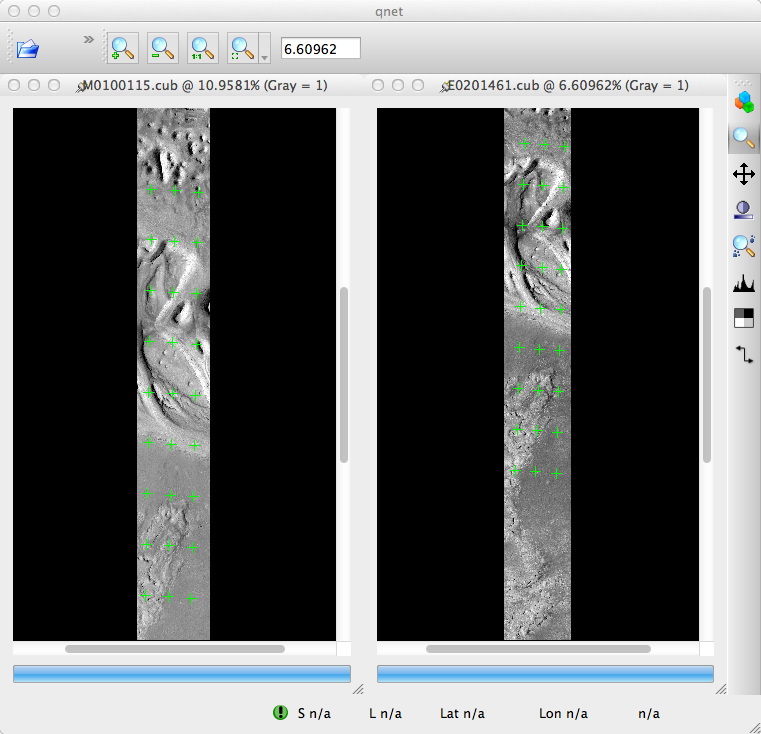
\includegraphics[width=5in]{images/qnet/Qnet_AfterAutoseed.png}
  \caption{A visualization of the features layed out by
    \texttt{autoseed} in \texttt{qnet}. Note that the marks do not
    cover the same features between images. This is due to the poor
    initial spice data for MOC imagery.}
  \label{fig:after_autoseed}
\end{figure}

\begin{verbatim}
  ISIS 3> autoseed fromlist=cube.lis overlaplist=overlap.lis    \
            onet=control.net deffile=autoseed.def networkid=moc \
            pointid=???? description=hrad_vallis
\end{verbatim}

The next step is to perform auto registration of these features
between the two images using \texttt{pointreg}. This program also
requires a settings file that describes how to do the automatic
search. Copy the text box below into a \textit{autoRegTemplate.def}
file.

\begin{verbatim}
   Object = AutoRegistration
    Group = Algorithm
      Name         = MaximumCorrelation
      Tolerance    = 0.7
    EndGroup

    Group = PatternChip
      Samples = 21
      Lines   = 21
      MinimumZScore = 1.5
      ValidPercent = 80
    EndGroup

    Group = SearchChip
      Samples = 75
      Lines   = 1000
    EndGroup
  EndObject
\end{verbatim}

The search chip defines the search range for which \texttt{pointreg}
will look for matching imagery. The pattern chip is simply the kernel
size of the matching template. The search range is specific for this
image pair. The control network result after \texttt{autoseed} had a
large vertical offset in the ball park of 500 px. The large
misalignment dictated the need for the large search in the lines
direction. Use \texttt{qnet} to get an idea for what the pixel shifts
look like in your stereo pair to help you decide on a search range. In
this example, only one measurement failed to match automatically. Here
are the arguments to use in this example of \texttt{pointreg}.

\begin{verbatim}
  ISIS 3> pointreg fromlist=cube.lis cnet=control.net             \
             onet=control_pointreg.net deffile=autoRegTemplate.def
\end{verbatim}

The third step is to manually edit the control and verify the
measurements in \texttt{qnet}. Type \texttt{qnet} in the terminal and
then open \textit{cube.lis} and lastly
\textit{control\_pointreg.net}. From the Control Network Navigator
window, click on the first point listed as \textit{0001}. That opens a
third window called the Qnet Tool. That window will allow you to play
a flip animation that shows alignment of the feature between the two
images. Correcting a measurement is performed by left clicking in the
right image, then clicking \textit{Save Measure}, and finally
finishing by clicking \textit{Save Point}.

In this tutorial, measurement \textit{0025} ended up being
incorrect. Your number may vary if you used different settings than
the above or if MOC spice data has improved since this writing. When
finished, go back to the main Qnet window. Save the final control
network as \textit{control\_qnet.net} by clicking on \textit{File},
and then \textit{Save As}.

\begin{figure}[ht]
  \centering
  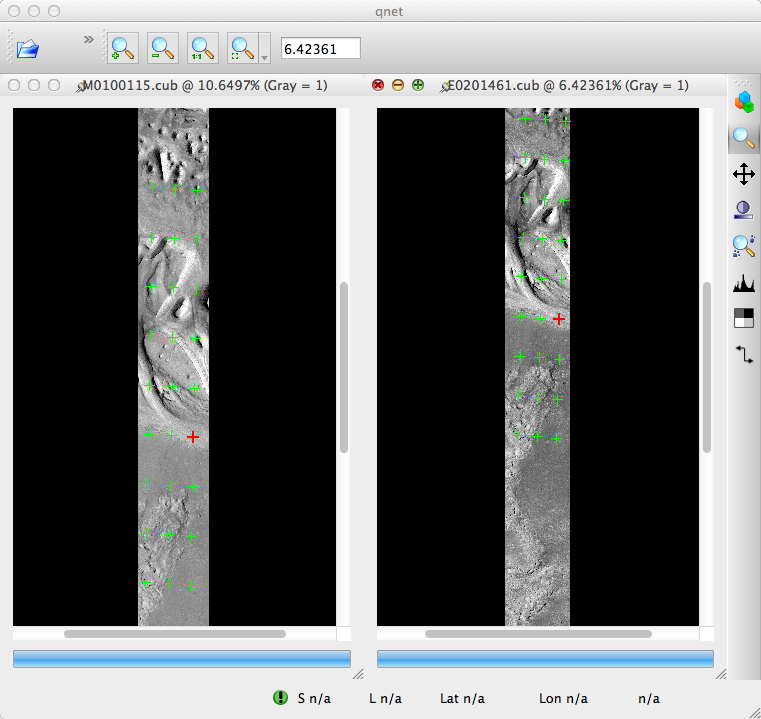
\includegraphics[width=5in]{images/qnet/Qnet_AfterQnetManual.png}
  \caption{A visualization of the features after manual editing in
    \texttt{qnet}. Note that the marks now appear in the same location
    between images.}
  \label{fig:after_autoseed}
\end{figure}

Once the control network is finished, it is finally time to start
bundle adjustment. Here's what the call to \texttt{jigsaw} looks like:

\begin{verbatim}
  ISIS 3> jigsaw fromlist=cube.lis update=yes twist=no radius=yes \
             cnet=control_qnet.net onet=control_ba.net
\end{verbatim}

The update option defines that we would like to update the camera
pointing, if our bundle adjustment converges. The \textit{twist=no}
says to not solve for the camera rotation about the camera bore. That
property is usually very well known as it is critical for integrating
an image with a line-scan camera. The \textit{radius=yes} means that
the radius of the 3D features can be solved for. Using no will force
the points to use height values from another source, usually LOLA or
MOLA.

The above command will spew out a bunch of diagnostic information from
every iteration of the optimization algorithm. The most important
feature to look at is the \textit{sigma0} value. It represents the mean of
pixel errors in the control network. In our run, the initial error was
1065 px and the final solution had an error of 1.1 px.

Producing a DEM using the newly created camera corrections is the same
as covered in the Tutorial on page \pageref{ch:tutorial}. When using
\texttt{jigsaw}, it modifies a copy of the spice data that is stored
internally to the cube file. Thus when we want to create a DEM using
the correct camera geometry, no extra information needs to be given to
\texttt{stereo} since it is already contained in the file. In the
event a mistake has been made, \texttt{spiceinit} will overwrite the
spice data inside a cube file and provide the original uncorrected
camera pointings.

\begin{verbatim}
  ISIS 3> stereo E0201461.cub M0100115.cub bundled/bundled
\end{verbatim}

%% \subsection{Processing with Ground Control Points}

%% Ground control point files describe a single point in the world
%% that is seen by 1 or more cameras. How they are measured in the
%% first place is up to the user. We use a manual process of comparing
%% each image to a respected map projected image and then recording
%% the latitude, longitude, and altitude of the point(s). The maps to
%% register against can be anything, but it is recommended to register
%% against a product with a high amount of cartographic stability and
%% accuracy.  For terrestrial work, we would use a \ac{USGS} product
%% that can provide imagery that is registered to LIDAR height
%% measurements.

%% Unlike match files, ground control points must specifically be given
%% to \texttt{isis\_adjust} from the command line, but in no particular
%% order. Ground control point files are written with the extension
%% \texttt{.gcp}. Below is an example of a ground control point file that
%% was created to control a series of Apollo Metric Camera images from
%% several Apollo 15 orbits.

%% \begin{verbatim}
%%     -52.8452 27.2561 1735999 300 300 500
%%     sub4-AS15-M-2086.cub     210.9   3565.0
%%     sub4-AS15-M-2087.cub     1476.9  3579.0
%%     sub4-AS15-M-2088.cub     2798.9  3586.8
%%     sub4-AS15-M-2089.cub     4133.5  3588.6
%%     sub4-AS15-M-2344.cub     906.9   3874.8
%%     sub4-AS15-M-2345.cub     2204.2  3913.9
%%     sub4-AS15-M-2482.cub     939.8   4348.0
%%     sub4-AS15-M-2483.cub     2282.0  4340.7
%%     sub4-AS15-M-2484.cub     3642.1  4330.9
%% \end{verbatim}

%% The first line of a \texttt{.gcp} file is like a header line and
%% is different from the remaining lines.  The first line defines the
%% world location of the ground control point, and the rest of the
%% lines define the image locations of the ground control points. Here
%% are what the columns mean for the first line.

%% \begin{myindentpar}{2cm}
%% \begin{description}
%%   \item[Column 1:] Longitude in degrees
%%   \item[Column 2:] Latitude in degrees
%%   \item[Column 3:] Radius in meters
%%   \item[Column 4:] Sigma (or uncertainty) in meters for Local X axis
%%   \item[Column 5:] Sigma (or uncertainty) in meters for Local Y axis
%%   \item[Column 6:] Sigma (or uncertainty) in meters for Local Z axis
%% \end{description}
%% \end{myindentpar}

%% The other lines describe where this \ac{GCP} is found in each image:

%% \begin{myindentpar}{2cm}
%% \begin{description}
%%   \item[Column 1:] Image name
%%   \item[Column 2:] Sample (X) image measurement
%%   \item[Column 3:] Line (Y) image measurement
%% \end{description}
%% \end{myindentpar}

%% Make a {\tt .gcp} file for every ground control point, then be sure
%% to feed them as an input to {\tt isis\_adjust}. Remember that you
%% can scale the sigma of all ground control points by using the {\tt
%% -\/-gcp-scalar} flag. This can save time by allowing you to make
%% adjustments without needing to edit all of the files individually.

%\include{data_visualization} <-- we should add this someday!
\chapter{Data Processing Examples}
\label{ch:examples}

This chapter showcases a variety of results that are possible when
processing different data sets with the Stereo Pipeline. It is also a
shortened guide that shows the commands and stereo.default files used
to process data. We hope that these are useful templates that will get
you started in processing your own data.

\section{Guidelines for Selecting Stereo Pairs}

When choosing image pairs to process, images that are taken with
similar viewing angles, lighting conditions, and significant surface
coverage overlap are best suited for creating terrain
models. Depending on the characteristics of the mission data set and
the individual images, the degree of acceptable variation will
differ. Significant differences between image characteristics
increases the liklihood of stereo matching error and artifacts, and
these errors will propagate through to the resulting data products.

Although images do not need to be map projected before running the
\texttt{stereo} program, we recommend that you do run {\tt cam2map}
beforehand, especially for image pairs that contain large topographic
variation (and therefore large disparity differences across the scene,
\emph{e.g. Valles Marineris}).  Map projection is especially necessary
when processing HiRISE images. This removes the large disparity
differences between HiRISE images and leaves only the small detail for
the Stereo Pipeline to compute. Remember that ISIS can work backwards
through a map-projection when applying the camera model, so the
geometric integrity of your images will not be sacrified if you map
project first.

Excessively noisy images will not correlate well, so images should be
photometrically calibrated in whatever fashion suits your purposes. If
there are photometric problems with the images, those photometric
defects can be misinterpreted as topography.

Remember, in order for \texttt{stereo} to process stereo pairs in ISIS
CUBE format, the images must have had SPICE data associated by running
ISIS's \texttt{spiceinit} program run on them first.

\section{Mars Reconaissance Orbiter HiRISE}

HiRISE is one of the most challenging cameras to use when making 3D
models because HiRISE exposures can be several gigabytes each. Working
with this data requires patience as it will take time.

One important fact to know about HiRISE is that it is composed of
multiple linear CCDs that are arranged side by side with some vertical
offsets. These offsets mean that the CCDs will view some of the same
terrain but at a slightly different time and a slightly different
angle. Mosiacing the CCDs together to a single image is not a simple
process and involves living with some imperfections.

At this time, we recommend mosaicking CCDs using the scripts available
at your institution (both USGS and University of Arizona have this
capability).  We are also providing a script that will take raw HiRISE
images and combine them into a mosaic. Our script takes all red CCDs
and projects them using the ISIS {\tt noproj} command into the
perspective of RED5 CCD. From there, {\tt hijitreg} is performed to
work out the relative offsets between CCDs. Finally the CCDs are
mosaicked together using the average offset listed from {\tt hijitreg}
using the {\tt handmos} command. Below is an outline of what our
script does.  It is based on the tutorial provided on the USGS ISIS
website.

\begin{verbatim}
    command outline
\end{verbatim}

Finally we recommend map projecting the product and normalizing both
images in the stereo pair using the same dynamic range. Notice that we
map project the second image using the same map settings and crop of
the first image. This means the images will share the same origin and
the {\tt stereo.default} search range can be centered around zero.

\begin{verbatim}
    cam2map f=first.cub t=first.map.cub
    cam2map f=second.cub map=first.map.cub t=second.map.cub matchmap=true
    bandnorm f=first.map.cub t=first.norm.cub
    bandnorm f=second.map.cub t=second.norm.cub
    ls first.norm.cub second.norm.cub > fromlist
    ls first.norm.cub > holdlist
    equalizer fromlist=fromlist holdlist=holdlist
    mkdir result
    stereo first.norm.equ.cub second.norm.equ.cub result/output
\end{verbatim}

In the future, it is our understanding that the HiRISE team will be
producing stitch but non-map--projected imagery to the PDS. If this
happens, most of the above commands will no longer be required.

\subsection{Columbia Hills}

The following description is taken and shortened from the HiRISE
instrument website.
\url{http://hirise.lpl.arizona.edu/PSP_001513_1655}

\begin{quotation}
This HiRISE image shows the landing site of the Mars Exploration Rover
Spirit. The impact crater in the upper left-hand portion of the image
is "Bonneville Crater," which was investigated by Spirit shortly after
landing. In the lower right-hand portion of the image is "Husband
Hill," a large hill that Spirit climbed and where it spent much of its
now nearly three-year mission.

The bright irregularly-shaped feature in the area north-west of
Bonneville Crater is Spirit's parachute, now lying on the Martian
surface. Near the parachute is the cone-shaped "backshell" that helped
protect Spirit's lander during its seven-month journey to Mars. The
backshell appears relatively undamaged by its impact with the martian
surface. Wrinkles and folds in the parachute fabric are clearly
visible.

Immediately south west of Bonneville Crater shows Spirit's lander. The
crater in the upper left-hand portion of the image, just to the
northwest of the lander, is the one that the Mars Exploration Rover
team named "Sleepy Hollow."

The north rim of Bonneville Crater shows the damaged remnant of the
heat shield that protected the vehicle during the high-speed entry
through the Martian atmosphere. The heat shield impacted the surface
after being separated from the vehicle during the final stages of the
descent.

South of Husband Hill shows the current location of Spirit. Toward the
top of the image is "Home Plate," a plateau of layered rocks that
Spirit explored during the early part of its third year on
Mars. Spirit itself is clearly seen just to the southeast of Home
Plate. Also visible are the tracks made by the rover before it arrived
at its current location.

Written by: Steve Squyres
\end{quotation}

\subsubsection*{Screenshot}

\begin{figure}[h!]
\centering
  \subfigure[{\tt 3D Rendering}]{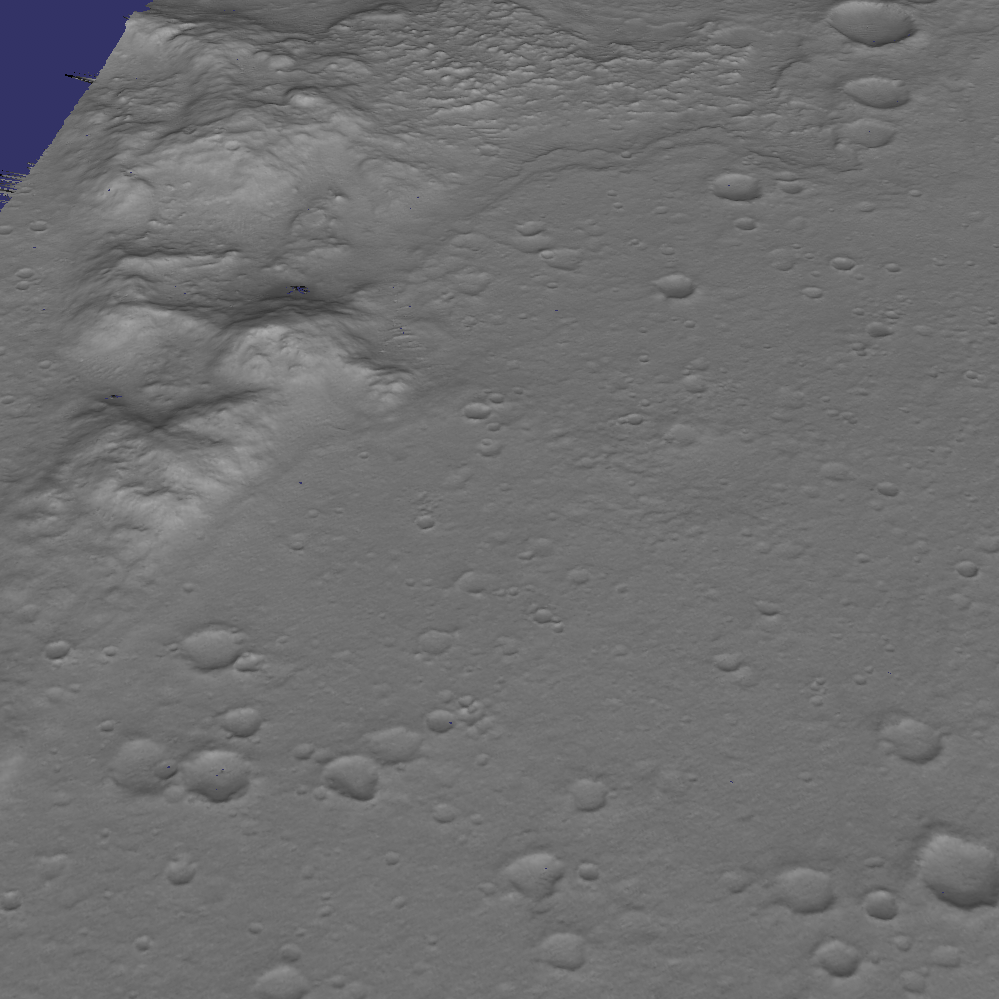
\includegraphics[width=3in]{images/examples/hirise/chills_hirise_example.png}}
  \hfil
  \subfigure[{\tt KML Screenshot}]{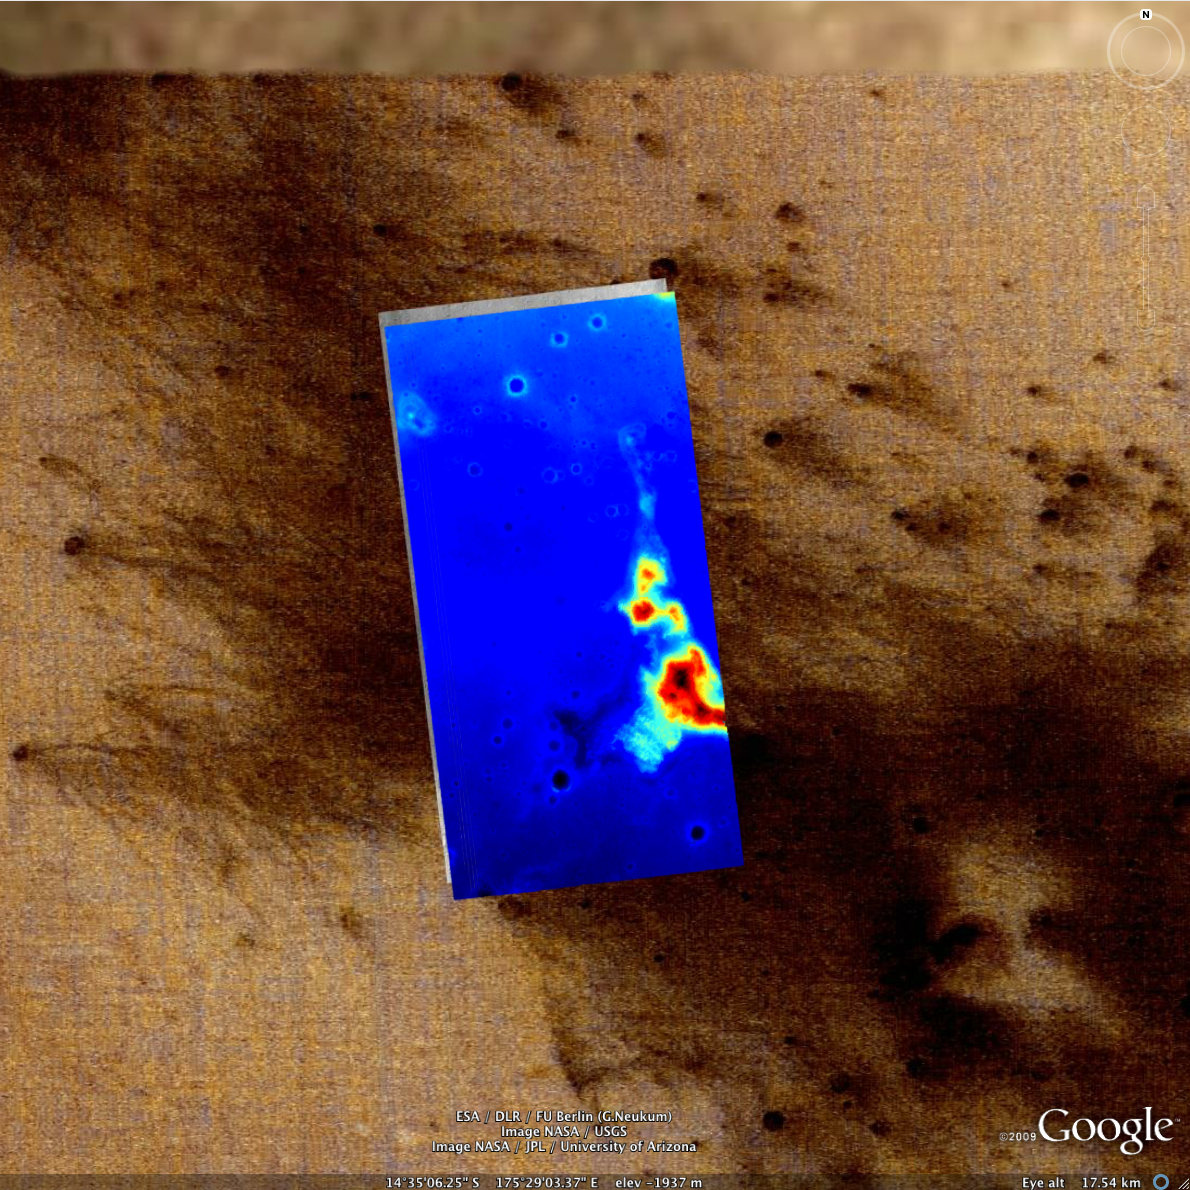
\includegraphics[width=3in]{images/examples/hirise/chills_hirise_ge_example.png}}
\caption{Example output using HiRISE images PSP\_001513\_1655 and
  PSP\_001777\_1650 of East Mareotis Tholus.}
\label{fig:hirise_chills_example}
\end{figure}

\subsubsection*{Commands}

\begin{verbatim}
    % Download all of the RED IMG for PSP_001513_1655 & %
    %                                 PSP_001777_1650   %
    ~/HiRISE_stitch.py PSP_001513_1655_RED0_0.IMG
    ~/HiRISE_stitch.py PSP_001777_1650_RED0_0.IMG
    cam2map from=PSP_001513_1655_REDmosaic.norm.cub to=PSP_001513_1655_REDmosaic.map.cub
    cam2map from=PSP_001777_1650_REDmosaic.norm.cub map=PSP_001513_1655_REDmosaic.map.cub ...
            to=PSP_001777_1650_REDmosaic.norm.cub matchmap=true
    bandnorm from=PSP_001513_1655_REDmosaic.map.cub to=PSP_001513_1655_REDmosaic.map.norm.cub
    bandnorm from=PSP_001777_1650_REDmosaic.map.cub to=PSP_001777_1650_REDmosaic.map.norm.cub
    ls *.map.norm.cub > fromlist
    ls *1513*.map.norm.cyb > holdlist
    equalizer fromlist=fromlist holdlist=holdlist
    rm *REDmosaic.map.norm.cub *REDmosaic.map.cub
    mkdir result
    stereo PSP_001513_1655.map.norm.equ.cub PSP_001777_1650.map.norm.equ.cub result/output
\end{verbatim}

\subsubsection*{Stereo Default}

\begin{verbatim}
    ### PREPROCESSING

    DO_INTERESTPOINT_ALIGNMENT 0
    INTERESTPOINT_ALIGNMENT_SUBSAMPLING 0
    DO_EPIPOLAR_ALIGNMENT 0

    FORCE_USE_ENTIRE_RANGE 1
    DO_INDIVIDUAL_NORMALIZATION 0

    PREPROCESSING_FILTER_MODE 2

    SLOG_KERNEL_WIDTH 1.5

    ### CORRELATION

    COST_MODE 0
    COST_BLUR 0

    H_KERNEL 50
    V_KERNEL 50

    H_CORR_MIN 210
    H_CORR_MAX 450
    V_CORR_MIN -320
    V_CORR_MAX 320

    SUBPIXEL_MODE 2

    SUBPIXEL_H_KERNEL 25
    SUBPIXEL_V_KERNEL 25

    ### FILTERING

    FILL_HOLES 1

    RM_H_HALF_KERN 5
    RM_V_HALF_KERN 5
    RM_MIN_MATCHES 60 # Units = percent
    RM_THRESHOLD 3
    RM_CLEANUP_PASSES 1

    ### DOTCLOUD

    NEAR_UNIVERSE_RADIUS 0.0
    FAR_UNIVERSE_RADIUS 0.0
\end{verbatim}

\subsection{East Mareotis Tholus}

The description is taken from the HiRISE instrument website.
\url{http://hirise.lpl.arizona.edu/PSP_001760_2160}

\begin{quotation}
East Mareotis Tholus is a small volcano in Tempe Terra, Mars. This
area is on the northeast edge of the Tharsis bulge that was built up
by many large and small volcanoes.

One of the many questions we hope to address with HiRISE is the
relative roles of the giant shield volcanoes (such as Olympus Mons)
and smaller volcanic features (such as East Mareotis Tholus).

The anaglyph covers 4.4 x 6.9 km (2.7 x 4.9 miles) and the topography
can be viewed using red-blue glasses. The elongated pit at the summit
of the volcano is where the lava issued forth. The large circular hole
just to the SW of the vent is an impact crater. The gouges in the
ground to the SE of the volcano are tectonic fissures (called graben)
that are now filled with sand dunes. The area is covered with large
amounts of wind-blown dust, so it is not surprising that lava flows
and other smaller volcanic features are not visible.

However, the smooth shape of the volcano, and the lack of lava layers
exposed in the impact crater, allow for the possiblity that this
volcano is composed largely of ash, rather than lava flows.

Written by: Laszlo P. Keszthelyi
\end{quotation}

\subsubsection*{Screenshot}

\begin{figure}[h!]
\centering
  \subfigure[{\tt 3D Rendering}]{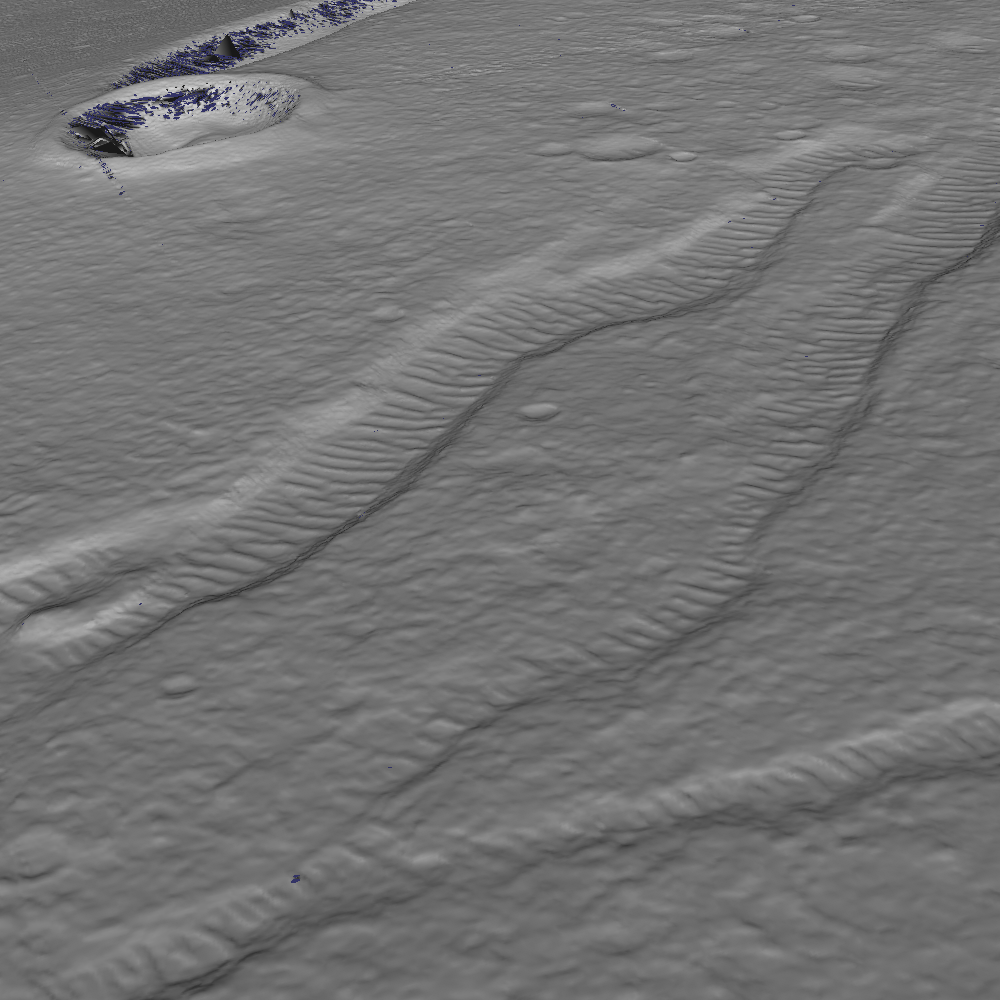
\includegraphics[width=3in]{images/examples/hirise/emare_example.png}}
  \hfil
  \subfigure[{\tt KML Screenshot}]{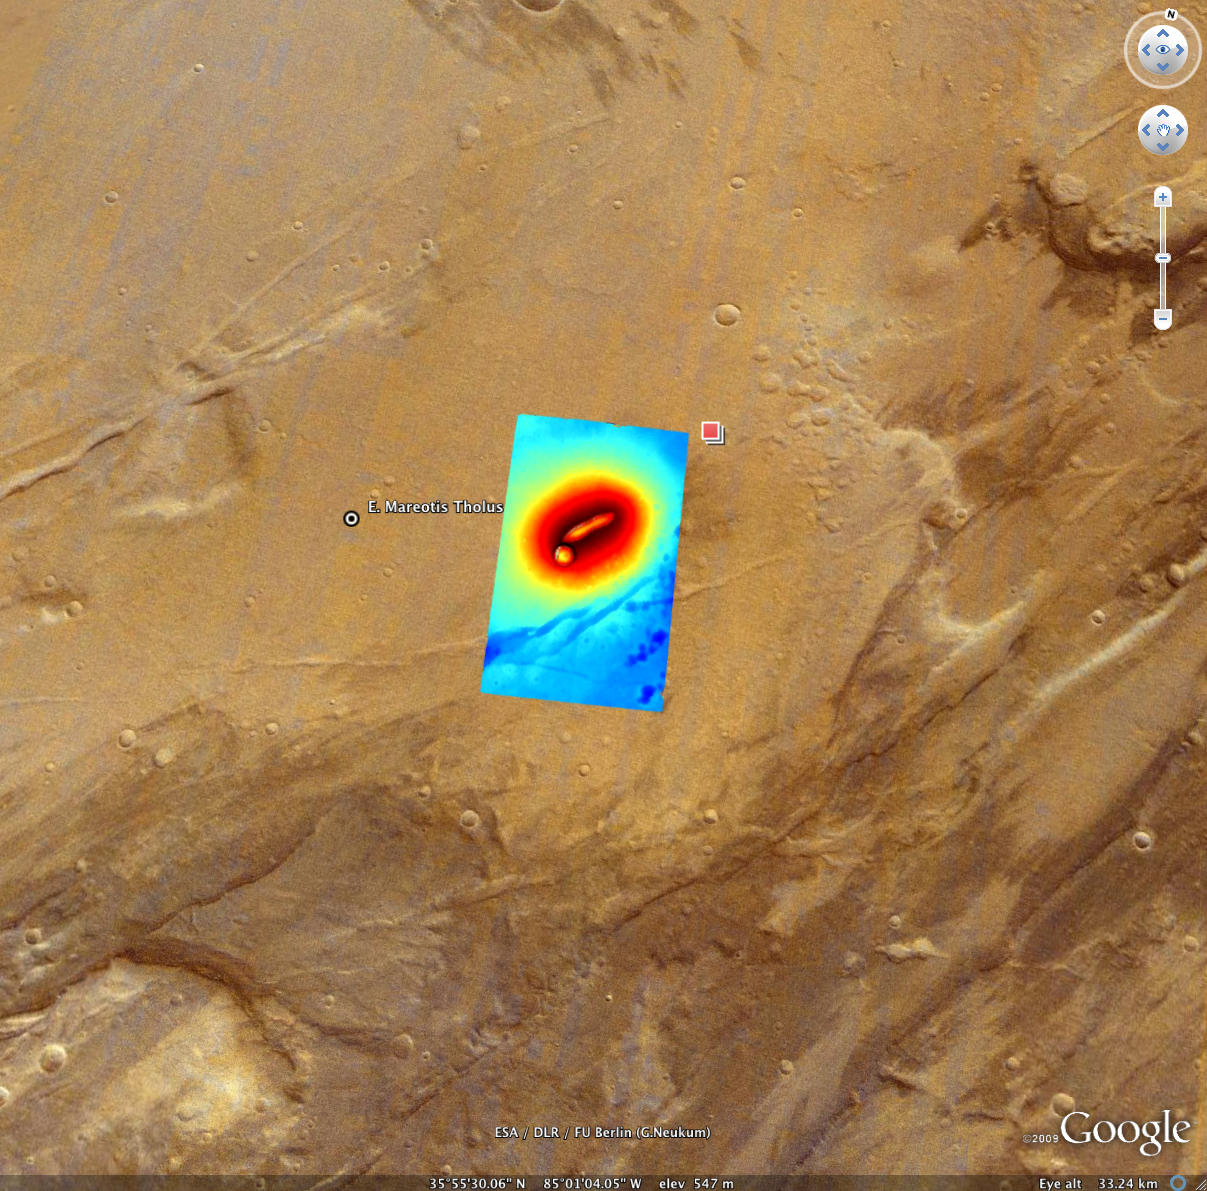
\includegraphics[width=3in]{images/examples/hirise/emare_ge_example.png}}
\caption{Example output using HiRISE images PSP\_001364\_2160 and
  PSP\_001760\_2160 of East Mareotis Tholus.}
\label{fig:hirise_emare_example}
\end{figure}

\subsubsection*{Commands}

\begin{verbatim}
    % Download all of the RED IMG for PSP_001364_2160 & %
    %                                 PSP_001760_2160   %
    ~/HiRISE_stitch.py PSP_001364_2160_RED0_0.IMG
    ~/HiRISE_stitch.py PSP_001760_2160_RED0_0.IMG
    cam2map from=PSP_001364_2160_REDmosaic.norm.cub to=PSP_001364_2160_REDmosaic.map.cub
    cam2map from=PSP_001760_2160_REDmosaic.norm.cub map=PSP_001364_2160_REDmosaic.map.cub ...
            to=PSP_001760_2160_REDmosaic.map.cub matchmap=true
    bandnorm from=PSP_001364_2160_REDmosaic.map.cub to=PSP_001364_2160_REDmosaic.map.norm.cub
    bandnorm from=PSP_001760_2160_REDmosaic.map.cub to=PSP_001760_2160_REDmosaic.map.norm.cub
    ls *.map.norm.cub > fromlist
    ls *1760*.map.norm.cub > holdlist
    equalizer fromlist=fromlist holdlist=holdlist
    rm *REDmosaic.map.norm.cub *REDmosaic.map.cub
    mkdir result
    stereo PSP_001364_2160.map.norm.equ.cub PSP_001760_2160.map.norm.equ.cub result/output
\end{verbatim}

\subsubsection*{Stereo Default}

\begin{verbatim}
    ### PREPROCESSING

    DO_INTERESTPOINT_ALIGNMENT 0
    INTERESTPOINT_ALIGNMENT_SUBSAMPLING 0
    DO_EPIPOLAR_ALIGNMENT 0

    FORCE_USE_ENTIRE_RANGE 1
    DO_INDIVIDUAL_NORMALIZATION 0

    PREPROCESSING_FILTER_MODE 2

    SLOG_KERNEL_WIDTH 1.5

    ### CORRELATION

    COST_BLUR 0
    COST_MODE 0

    H_KERNEL 25
    V_KERNEL 25

    H_CORR_MIN -80
    H_CORR_MAX 150
    V_CORR_MIN -80
    V_CORR_MAX 50

    SUBPIXEL_MODE 0

    SUBPIXEL_H_KERNEL 25
    SUBPIXEL_V_KERNEL 25

    ### FILTERING

    FILL_HOLES 1

    RM_H_HALF_KERN 5
    RM_V_HALF_KERN 5
    RM_MIN_MATCHES 60 # Units = percest
    RM_THRESHOLD 3
    RM_CLEANUP_PASSES 1

    ### DOTCLOUD

    NEAR_UNIVERSE_RADIUS 0.0
    FAR_UNIVERSE_RADIUS 0.0
\end{verbatim}

\subsection{North Terra Meridiani Crop}

HiRISE website only has to say that this is `Layered Materials within
a Small Crater'. Hopefully you'll still agree that this is cool.

\subsubsection*{Screenshot}

\begin{figure}[h!]
\centering
  \subfigure[{\tt 3D Rendering}]{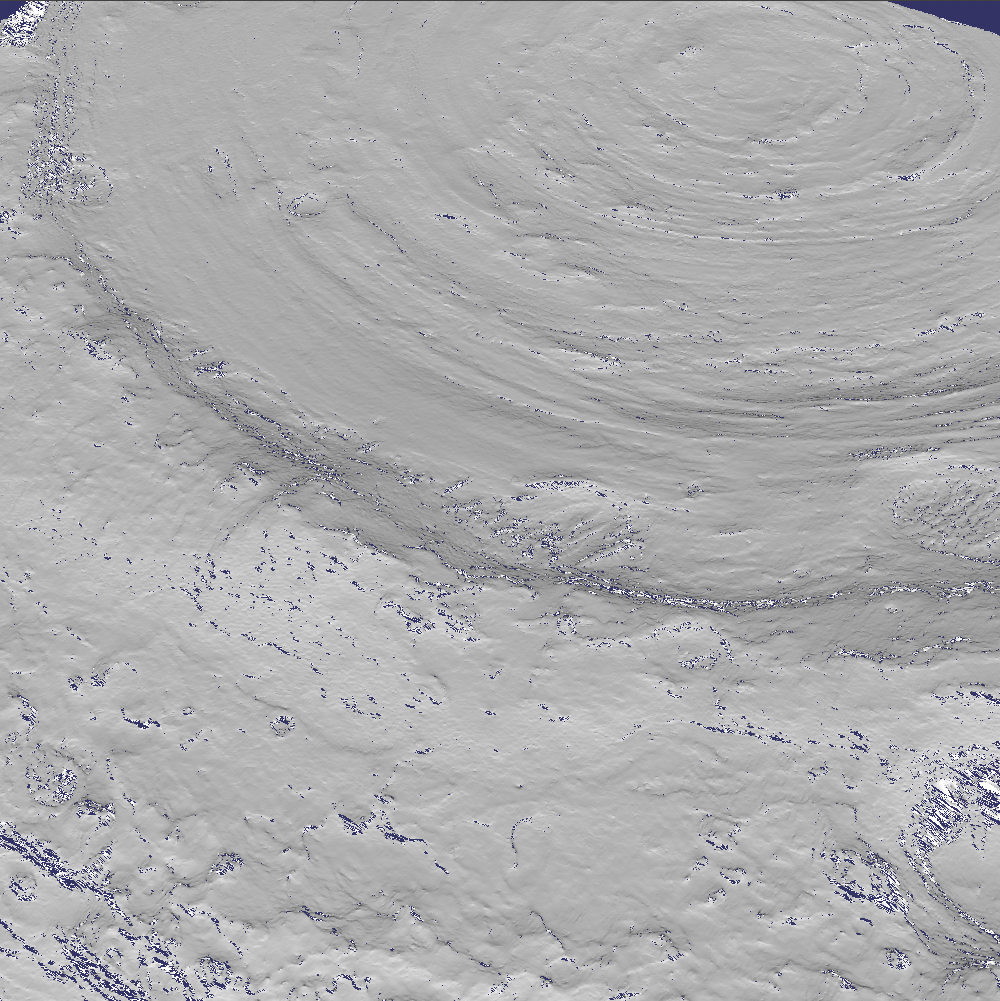
\includegraphics[width=3in]{images/examples/hirise/nterra_example.png}}
  \hfil
  \subfigure[{\tt KML Screenshot}]{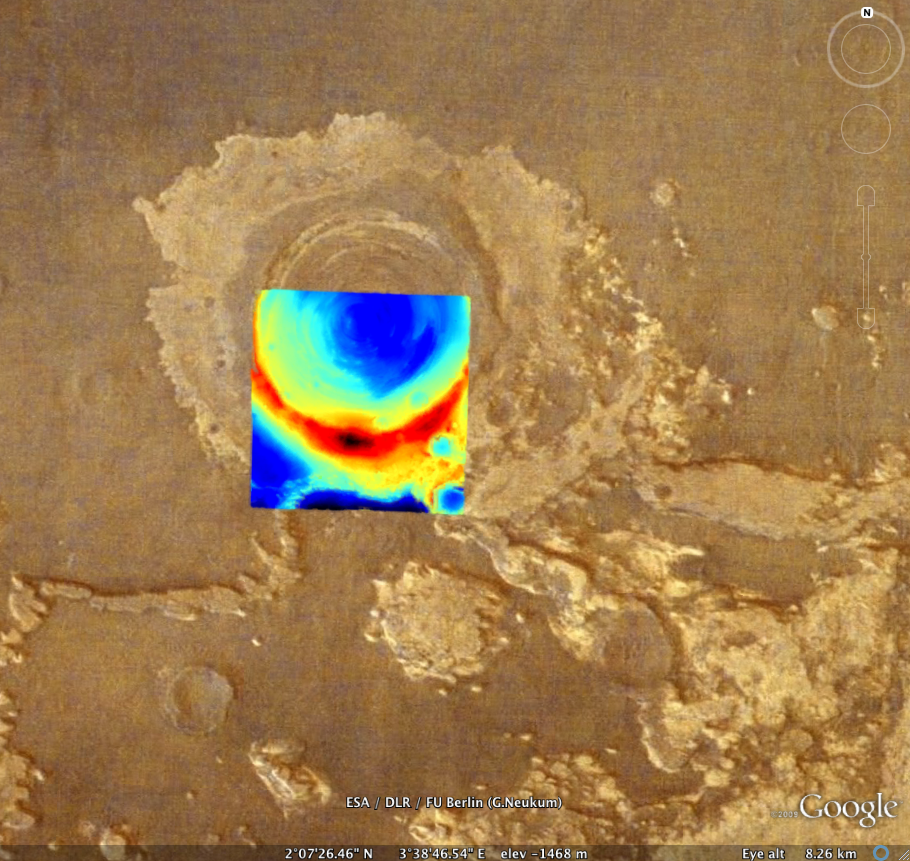
\includegraphics[width=3in]{images/examples/hirise/nterra_ge_example.png}}
\caption{Example output using cropped HiRISE data of North Terra Meridiani.}
\label{fig:hirise_nterra_example}
\end{figure}

\subsubsection*{Commands}

Notice here that we have applied a crop to select a subset of these
HiRISE images that we are interested in.  Cropping is often an
efficient way to go because it greatly reduces the amount of
computation necessary to get results in a limited area.

\begin{verbatim}
    % Download all of the IMG for PSP_001981_1825 & %
    %                             PSP_002258_1825   %
    ~/HiRISE_stitch.py PSP_001981_1825_RED0_0.IMG
    ~/HiRISE_stitch.py PSP_002258_1825_RED0_0.IMG
    cam2map from=PSP_001981_1825_REDmosaic.norm.cub to=PSP_001981_1825_REDmosaic.map.cub
    cam2map from=PSP_002258_1825_REDmosaic.norm.cub map=PSP_001981_1825_REDmosaic.map.cub ...
            to=PSP_002258_1825_REDmosaic.map.cub matchmap=true
    bandnorm from=PSP_001981_1825_REDmosaic.map.cub to=PSP_001981_1825_REDmosaic.map.norm.cub
    bandnorm from=PSP_002258_1825_REDmosaic.map.cub to=PSP_002258_1825_REDmosaic.map.norm.cub
    ls *.map.norm.cub > fromlist
    ls *1981*.map.norm.cub > holdlist
    equalizer fromlist=fromlist holdlist=holdlist
    crop from=PSP_001981_1825_REDmosaic.map.norm.equ.cub to=PSP_001981_1825.crop.cub ...
         sample=7497 line=41318 nsamp=10000 nline=10000
    crop from=PSP_002258_1825_REDmosaic.map.norm.equ.cub to=PSP_002258_1825.crop.cub ...
         sample=7982 line=41310 nsamp=10000 nline=10000
    rm *REDmosaic*.cub
    mkdir result
    stereo PSP_001981_1825.crop.cub PSP_002258_1825.crop.cub result/output
\end{verbatim}

\subsubsection*{Stereo Default}

\begin{verbatim}
    ### PREPROCESSING

    DO_INTERESTPOINT_ALIGNMENT 0
    INTERESTPOINT_ALIGNMENT_SUBSAMPLING 0
    DO_EPIPOLAR_ALIGNMENT 0

    FORCE_USE_ENTIRE_RANGE 1
    DO_INDIVIDUAL_NORMALIZATION 0

    PREPROCESSING_FILTER_MODE 2

    SLOG_KERNEL_WIDTH 1.5

    ### CORRELATION

    COST_BLUR 21
    COST_MODE 2

    H_KERNEL 45
    V_KERNEL 45

    H_CORR_MIN -270
    H_CORR_MAX -70
    V_CORR_MIN -14
    V_CORR_MAX 26

    SUBPIXEL_MODE 0

    SUBPIXEL_H_KERNEL 25
    SUBPIXEL_V_KERNEL 25

    ### FILTERING

    FILL_HOLES 1

    RM_H_HALF_KERN 5
    RM_V_HALF_KERN 5
    RM_MIN_MATCHES 60 # Units = percent
    RM_THRESHOLD 3
    RM_CLEANUP_PASSES 1

    ### DOTCLOUD

    NEAR_UNIVERSE_RADIUS 0.0
    FAR_UNIVERSE_RADIUS 0.0
\end{verbatim}


\section{Mars Reconaissance Orbiter CTX}

\subsection{North Terra Meridiani}

\subsubsection*{Screenshot}

\begin{figure}[h!]
\centering
  \subfigure[{\tt 3D Rendering}]{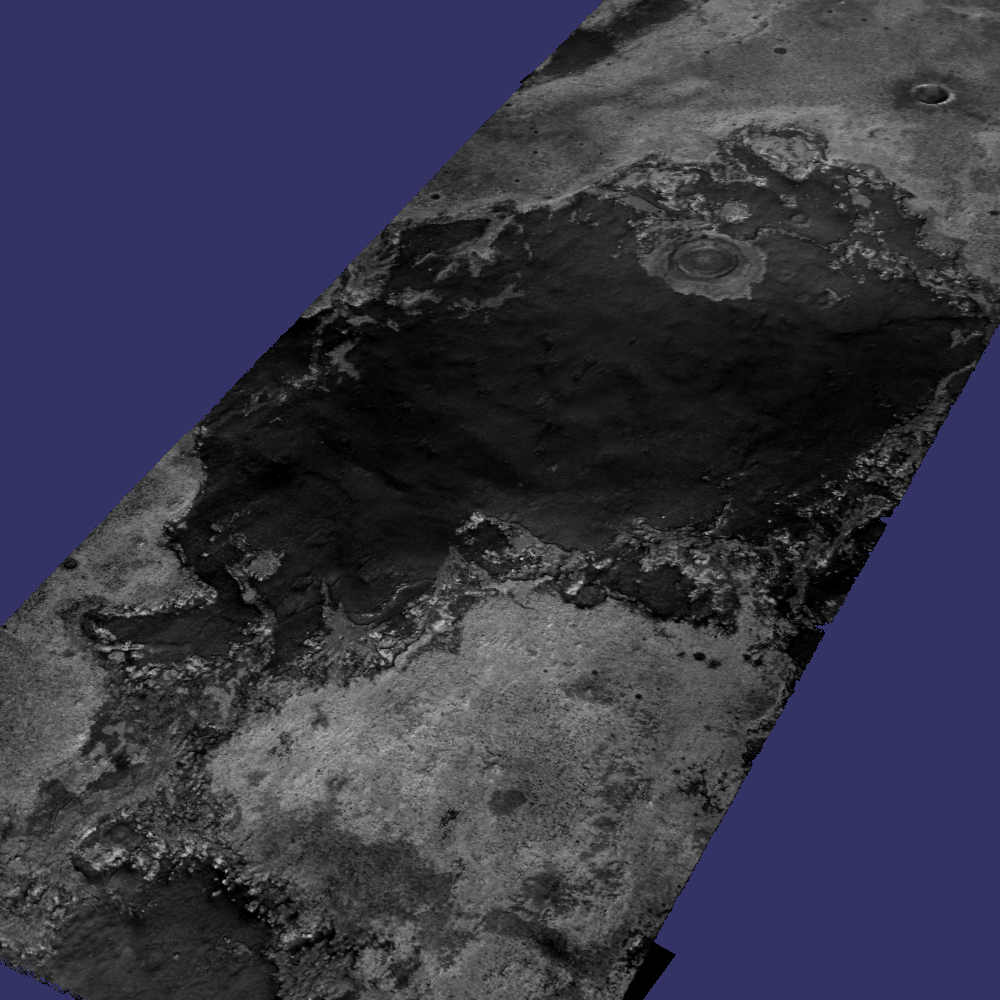
\includegraphics[width=3in]{images/examples/ctx/n_terra_meridiani_ctx.png}}
  \hfil
  \subfigure[{\tt KML Screenshot}]{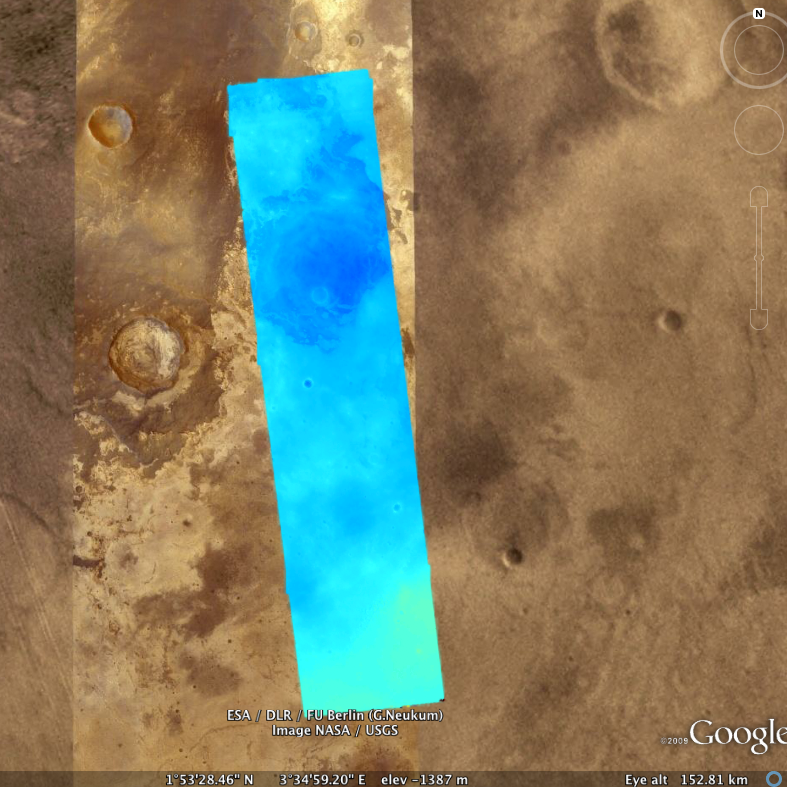
\includegraphics[width=3in]{images/examples/ctx/n_terra_meridiani_ctx_ge.png}}
\caption{Example output possible with the CTX imager aboard MRO.}
\label{fig:ctx_example}
\end{figure}

\subsubsection*{Commands}

\begin{verbatim}
    % Download P02_001981_1823_XI_02N356W.IMG &
    %          P03_002258_1817_XI_01N356W.IMG
    mroctx2isis from=P02_001981_1823_XI_02N356W.IMG to=P02_001981_1823_XI_02N356W.cub
    mroctx2isis from=P03_002258_1817_XI_01N356W.IMG to=P03_002258_1817_XI_01N356W.cub
    spiceinit from=P02_001981_1823_XI_02N356W.cub
    spiceinit from=P03_002258_1817_XI_01N356W.cub
    ctxcal from=P02_001981_1823_XI_02N356W.cub to=P02_001981_1823_XI_02N356W.cal.cub
    ctxcal from=P03_002258_1817_XI_01N356W.cub to=P03_002258_1817_XI_01N356W.cal.cub
    cam2map from=P02_001981_1823_XI_02N356W.cal.cub to=P02_001981_1823_XI_02N356W.map.cub
    cam2map from=P03_002258_1817_XI_01N356W.cal.cub to=P03_002258_1817_XI_01N356W.map.cub
\end{verbatim}

\subsubsection*{Stereo Default}

\begin{verbatim}
    ### PREPROCESSING

    DO_INTERESTPOINT_ALIGNMENT 1
    INTERESTPOINT_ALIGNMENT_SUBSAMPLING 0
    DO_EPIPOLAR_ALIGNMENT 0

    FORCE_USE_ENTIRE_RANGE 0
    DO_INDIVIDUAL_NORMALIZATION 0

    PREPROCESSING_FILTER_MODE 3

    SLOG_KERNEL_WIDTH 1.5

    ### CORRELATION

    COST_BLUR 0
    COST_MODE 2

    H_KERNEL 35
    V_KERNEL 35

    H_CORR_MIN -300
    H_CORR_MAX 300
    V_CORR_MIN -150
    V_CORR_MAX 150

    SUBPIXEL_MODE 3

    SUBPIXEL_H_KERNEL 21
    SUBPIXEL_V_KERNEL 21

    ### FILTERING

    FILL_HOLES 1

    RM_H_HALF_KERN 5
    RM_V_HALF_KERN 5
    RM_MIN_MATCHES 60 # Units = percest
    RM_THRESHOLD 3
    RM_CLEANUP_PASSES 1

    ### DOTCLOUD

    NEAR_UNIVERSE_RADIUS 0.0
    FAR_UNIVERSE_RADIUS 0.0
\end{verbatim}

\section{Mars Global Surveyor MOC-NA}

In the Stereo Pipeline Tutorial in Chapter~\ref{ch:tutorial}, we
showed you how to process a MOC-NA stereo pair that covered the
Galaxius Fluctus channel. In this section we will show you more
examples, some of which exhibit a problem common to stereo pairs from
linescan imagers: ``Spacecraft jitter'' is caused by oscillations on
the spacecraft due to the movement of other spacecraft hardware.  All
spacecraft wobble around to some degree but some, especially Mars
Global Surveyor, are particularly succeptible.

Jitter causes wave-like distortions along the track of the satellite
orbit in DEMs produced from linescan camera images.  This effect can
be very subtle or quite pronounced, so it is important to check you
data products carefully for any sign of this type of artifact. The
following examples will show the typical distortions created by this
problem.

Note that the science teams of HiRISE and LROC are actively working on
detecting and correctly modeling jitter in their respective SPICE
data. If they succeed in this, the distortions will still being in the
raw imagery, but the jitter will no longer produce ripple artifacts in
the DEMs produced using ours or other stereo reconstruction software.

\subsection{Ceraunius Tholus}

Ceraunius Tholus is a steep volcano that is part of the Uranius group
on Mars. It can be found at 23.96 N and 262.60 E. This DEM crosses the
volcano's caldera.

\subsubsection*{Screenshot}

\begin{figure}[h!]
\centering
  \subfigure[{\tt 3D Rendering}]{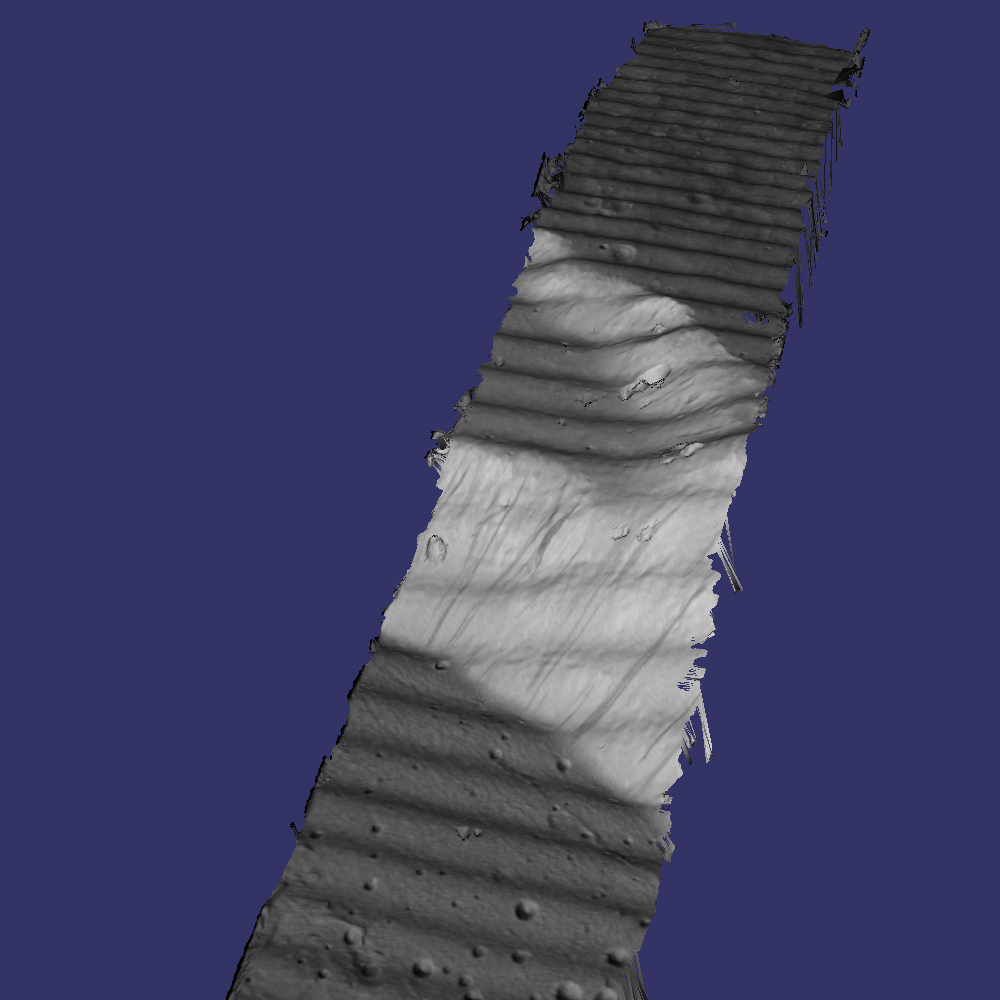
\includegraphics[width=3in]{images/examples/mocna/ceraunius_tholus_mocna.png}}
  \hfil
  \subfigure[{\tt KML Screenshot}]{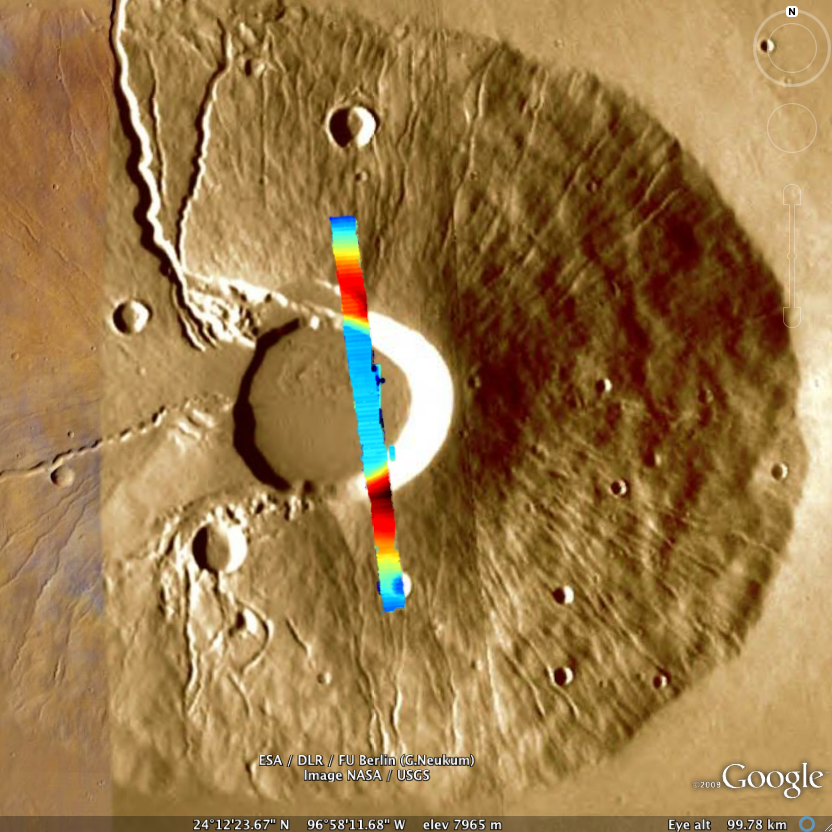
\includegraphics[width=3in]{images/examples/mocna/ceraunius_tholus_mocna_ge.png}}
\caption{Example output for MOC-NA of Ceraunius Tholus. Notice the presence of severe washboarding artifacts due to spacecraft ``jitter.''}
\label{fig:mocna_ceraunius_example}
\end{figure}

\subsubsection*{Commands}

\begin{verbatim}
    % Download M0806047.img & R0701361.img
    moc2isis f=M0806047.img t=M0806047.cub mapping=no
    moc2isis f=R0701361.img t=R0701361.cub mapping=no
    cam2map from=M0806047.cub to=M0806047.map.cub
    cam2map from=R0701361.cub map=M0806047.map.cub to=R0701361.map.cub matchmap=true
    mkdir result
    stereo M0806047.map.cub R0701361.map.cub result/output
\end{verbatim}

\subsubsection*{Stereo Default}

\begin{verbatim}
    ### PREPROCESSING

    DO_INTERESTPOINT_ALIGNMENT 0
    INTERESTPOINT_ALIGNMENT_SUBSAMPLING 0
    DO_EPIPOLAR_ALIGNMENT 0

    FORCE_USE_ENTIRE_RANGE 1
    DO_INDIVIDUAL_NORMALIZATION 1

    PREPROCESSING_FILTER_MODE 2

    SLOG_KERNEL_WIDTH 1.5

    ### CORRELATION

    COST_BLUR 12
    COST_MODE 2

    H_KERNEL 25
    V_KERNEL 25

    H_CORR_MIN -12
    H_CORR_MAX 26
    V_CORR_MIN -50
    V_CORR_MAX 15

    SUBPIXEL_MODE 2

    SUBPIXEL_H_KERNEL 21
    SUBPIXEL_V_KERNEL 21

    ### FILTERING

    FILL_HOLES 1

    RM_H_HALF_KERN 5
    RM_V_HALF_KERN 5
    RM_MIN_MATCHES 60 # Units = percent
    RM_THRESHOLD 3
    RM_CLEANUP_PASSES 1

    ### DOTCLOUD

    NEAR_UNIVERSE_RADIUS 0.0
    FAR_UNIVERSE_RADIUS 0.0
\end{verbatim}

\subsection{North Tharsis}

The Malin Space Science System's website describes this image as the
`Throughs and terraces in northern Tharsis'. This DEM is located at
20.20 N and 118.18 W on Mars.

\subsubsection*{Screenshot}

\begin{figure}[h!]
\centering
  \subfigure[{\tt 3D Rendering}]{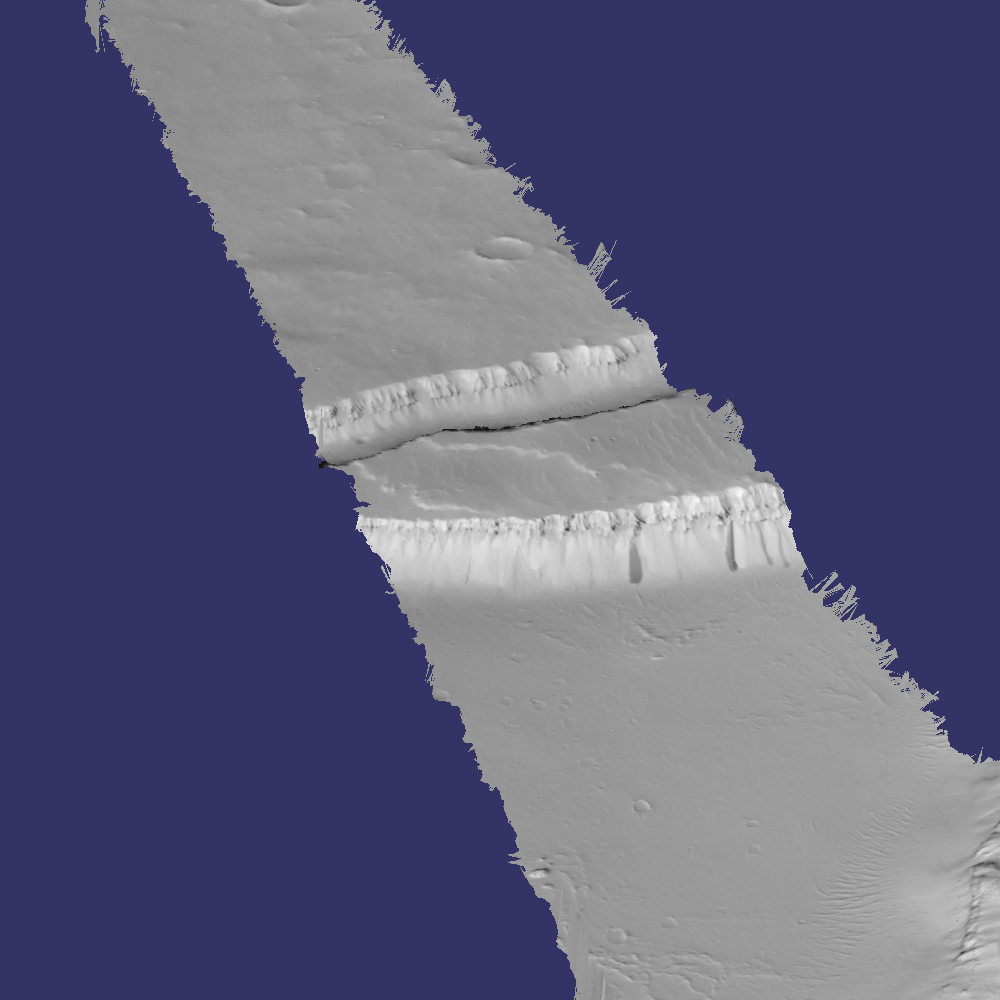
\includegraphics[width=3in]{images/examples/mocna/n_tharsis_mocna.png}}
  \hfil
  \subfigure[{\tt KML Screenshot}]{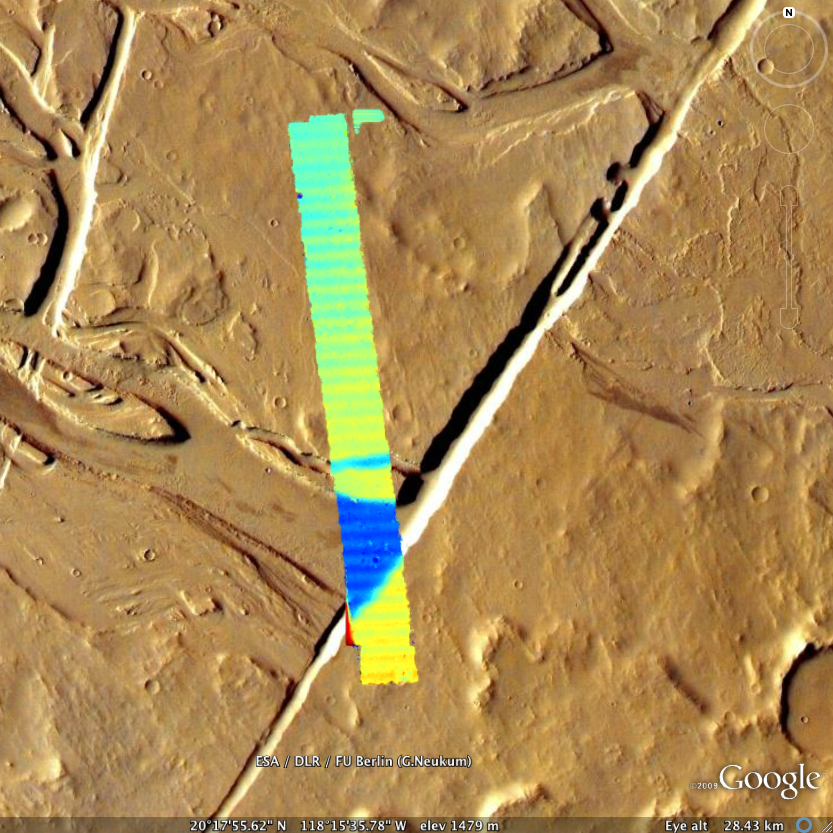
\includegraphics[width=3in]{images/examples/mocna/n_tharsis_mocna_ge.png}}
\caption{Example output for MOC-NA of North Tharsis.}
\label{fig:mocna_n_tharsis_example}
\end{figure}

\subsubsection*{Commands}

\begin{verbatim}
    % Download M0803097.img & S0701420.img
    moc2isis f=M0803097.img t=M0803097.cub mapping=no
    moc2isis f=S0701420.img t=S0701420.cub mapping=no
    cam2map from=M0803097.cub to=M0803097.map.cub
    cam2map from=S0701420.cub map=M0803097.map.cub to=S0701420.map.cub matchmap=true
    mkdr result
    stereo M0803097.map.cub S0701420.map.cub result/output
\end{verbatim}

\subsubsection*{Stereo Default}

\begin{verbatim}
    ### PREPROCESSING

    DO_INTERESTPOINT_ALIGNMENT 0
    INTERESTPOINT_ALIGNMENT_SUBSAMPLING 0
    DO_EPIPOLAR_ALIGNMENT 0

    FORCE_USE_ENTIRE_RANGE 1
    DO_INDIVIDUAL_NORMALIZATION 1

    PREPROCESSING_FILTER_MODE 2

    SLOG_KERNEL_WIDTH 1.5

    ### CORRELATION

    COST_BLUR 12
    COST_MODE 2

    H_KERNEL 25
    V_KERNEL 25

    H_CORR_MIN -50
    H_CORR_MAX 0
    V_CORR_MIN -85
    V_CORR_MAX 0

    SUBPIXEL_MODE 2

    SUBPIXEL_H_KERNEL 21
    SUBPIXEL_V_KERNEL 21

    ### FILTERING

    FILL_HOLES 1

    RM_H_HALF_KERN 5
    RM_V_HALF_KERN 5
    RM_MIN_MATCHES 60 # Units = percent
    RM_THRESHOLD 3
    RM_CLEANUP_PASSES 1

    ### DOTCLOUD

    NEAR_UNIVERSE_RADIUS 0.0
    FAR_UNIVERSE_RADIUS 0.0
\end{verbatim}


\section{Lunar Reconaissance Orbiter LROC-NA}

\subsection{Lee-Lincoln Scarp}

This stereo pair covers the Taurus-Littrow valley on the Moon where,
on December 11, 1972, the astronauts of Apollo 17 landed. However,
this stereo pair does not contain the landing site.  It is slightly
west; focusing on the Lee-Lincoln scarp that is on North Massif. The
scarp is an 80 m high feature that is the only visible sign of a deep
fault.

\subsubsection*{Screenshot}

\begin{figure}[h!]
\centering
  \subfigure[{\tt 3D Rendering}]{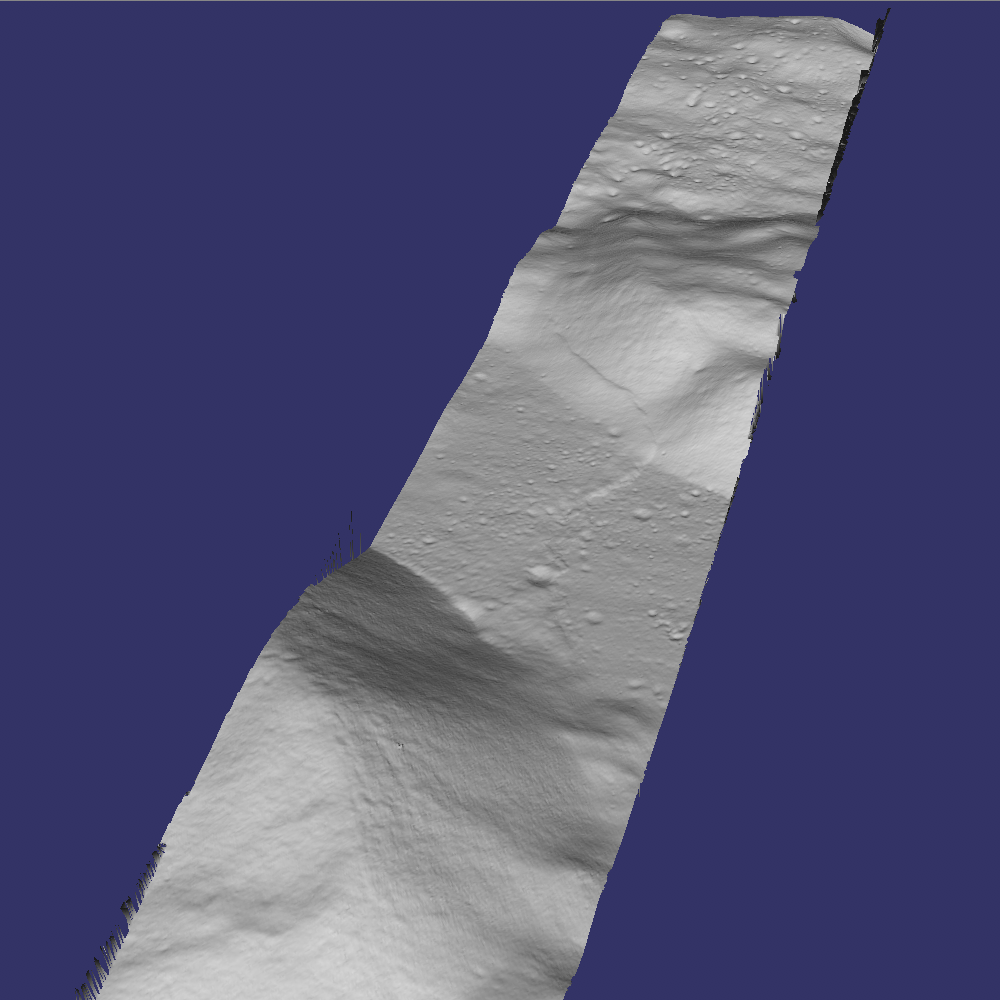
\includegraphics[width=3in]{images/examples/lrocna/lroc-na-example.png}}
  \hfil
  \subfigure[{\tt KML Screenshot}]{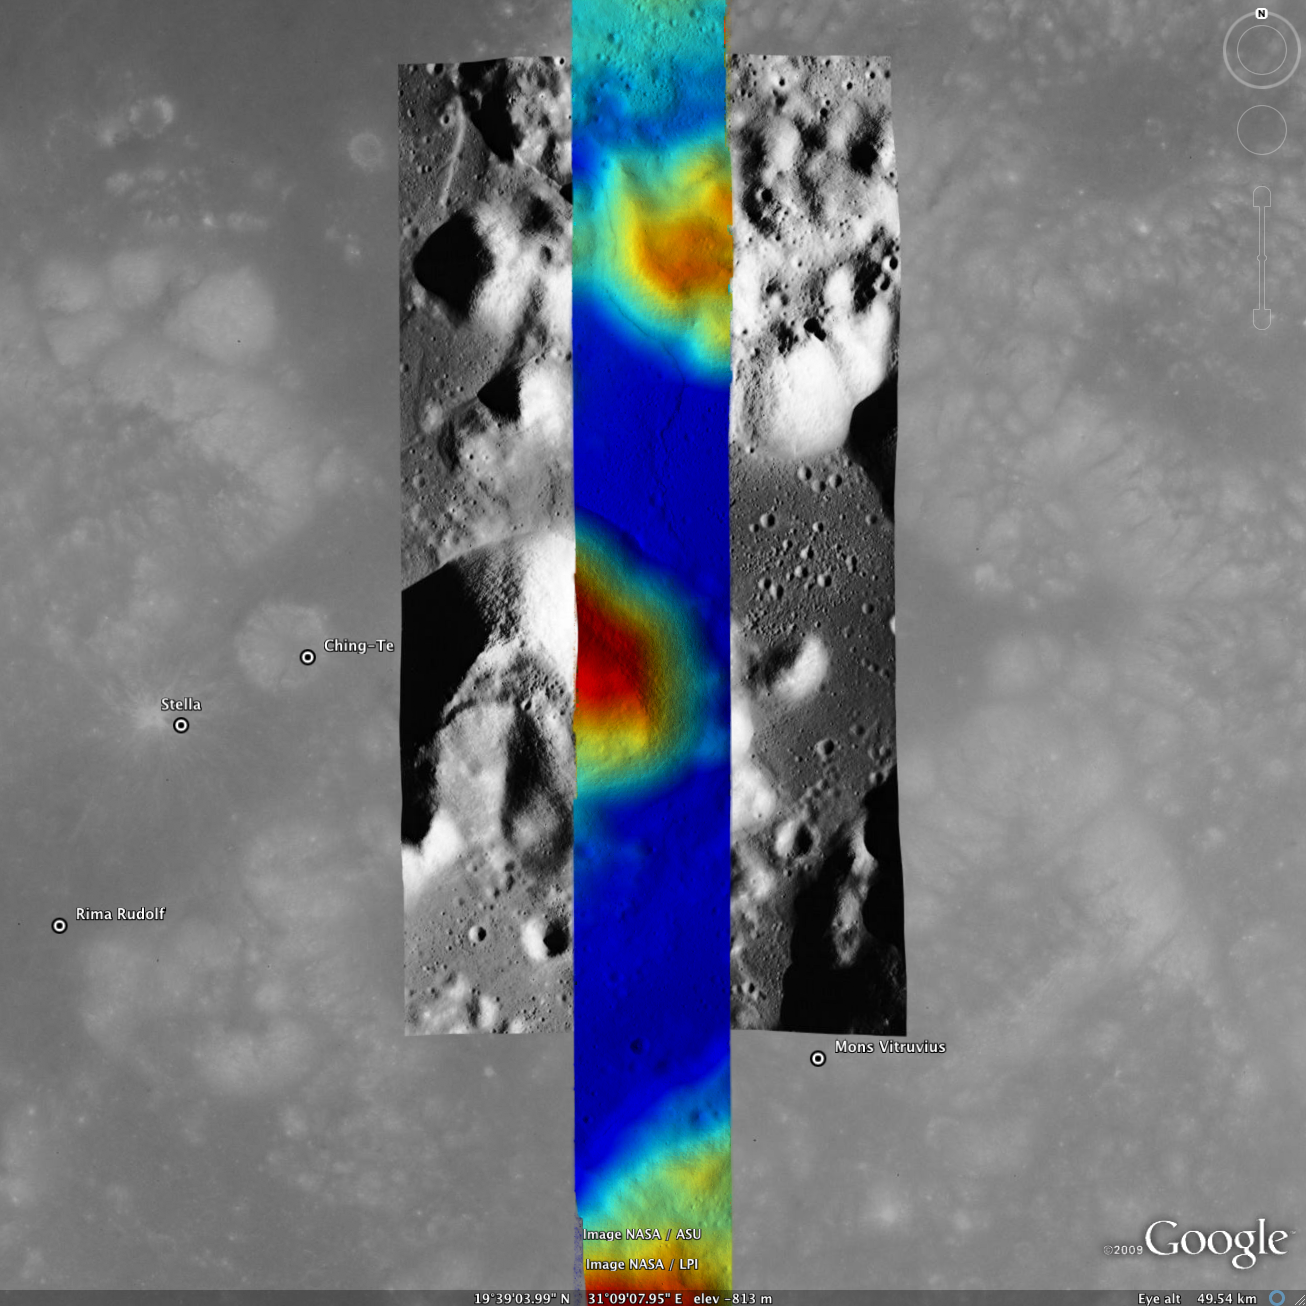
\includegraphics[width=3in]{images/examples/lrocna/lroc-na-ge_example.png}}
\caption{Example output possible with a LROC NA stereo pair, using only a single CCDs from observations.}
\label{fig:lroc-na-example}
\end{figure}

\subsubsection*{Commands}

\begin{verbatim}
    % Download nacl00002db8.* & nacl00004c86.*
    % process with unreleased tools to make cubes
    cam2map from=nacl00002db8.cub to=nacl00002db8.map.cub
    cam2map from=nacl00004c86.cub map=nacl00002db8.map.cub ...
            to=nacl00004c86.map.cub matchmap=true
    mkdir result
    stereo nacl00002db8.map.cub nacl00004c86.map.cub result/output
\end{verbatim}

\subsubsection*{Stereo Default}

\begin{verbatim}
    ### PREPROCESSING

    DO_INTERESTPOINT_ALIGNMENT 0
    INTERESTPOINT_ALIGNMENT_SUBSAMPLING 0
    DO_EPIPOLAR_ALIGNMENT 0

    FORCE_USE_ENTIRE_RANGE 1
    DO_INDIVIDUAL_NORMALIZATION 0

    PREPROCESSING_FILTER_MODE 2

    SLOG_KERNEL_WIDTH 1.5

    ### CORRELATION

    COST_BLUR 12
    COST_MODE 2

    H_KERNEL 29
    V_KERNEL 29

    H_CORR_MIN -425
    H_CORR_MAX 150
    V_CORR_MIN -100
    V_CORR_MAX 100

    SUBPIXEL_MODE 2

    SUBPIXEL_H_KERNEL 25
    SUBPIXEL_V_KERNEL 25

    ### FILTERING

    FILL_HOLES 1

    RM_H_HALF_KERN 5
    RM_V_HALF_KERN 5
    RM_MIN_MATCHES 60 # Units = percent
    RM_THRESHOLD 3
    RM_CLEANUP_PASSES 1

    ### DOTCLOUD

    NEAR_UNIVERSE_RADIUS 0.0
    FAR_UNIVERSE_RADIUS 0.0
\end{verbatim}


\section{Apollo 15 Metric Camera Images}

Apollo Metric images were all taken at regular intervals, which means
that the same stereo.default can be used for all sequential pairs of
images. Apollo Metric images are ideal for stereo processing.  They
produce consistent, excellent results.

The scans performed by ASU are sufficiently detailed to exhibit film
grain at the highest resolution.  The amount of noise at the full
resolution is not helpful for the correlator, so we recommended
subsampling the images by a factor of 4.

Currently the tools to ingest Apollo TIFFs into ISIS are not
available, but these images should soon be released into the PDS for
general public usage.

\subsection{Ansgarius C}

Ansgarius C is a small crater on the west edge of the farside of the
Moon near the equator. It is east of Kapteyn A and B.

\subsubsection*{Screenshot}

\begin{figure}[h!]
\centering
  \subfigure[{\tt 3D Rendering}]{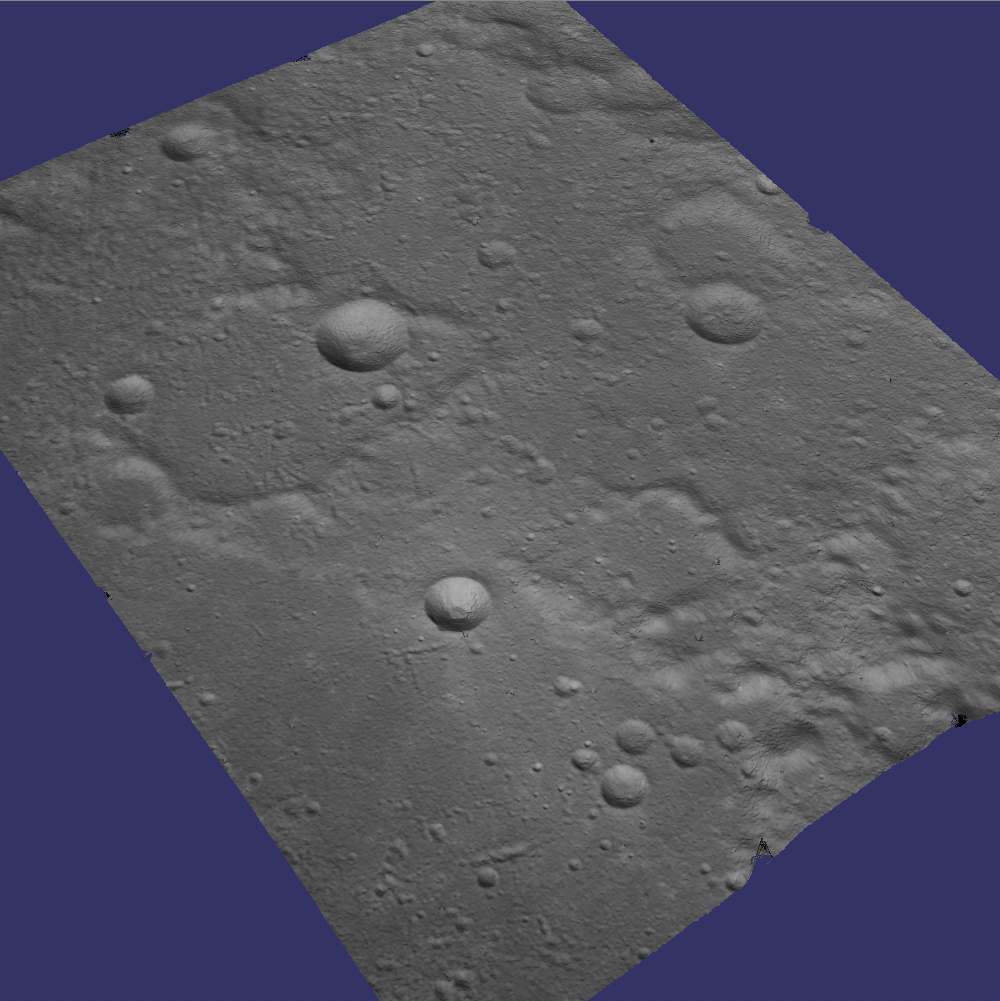
\includegraphics[width=3in]{images/examples/metric/metric_example.png}}
  \hfil
  \subfigure[{\tt KML Screenshot}]{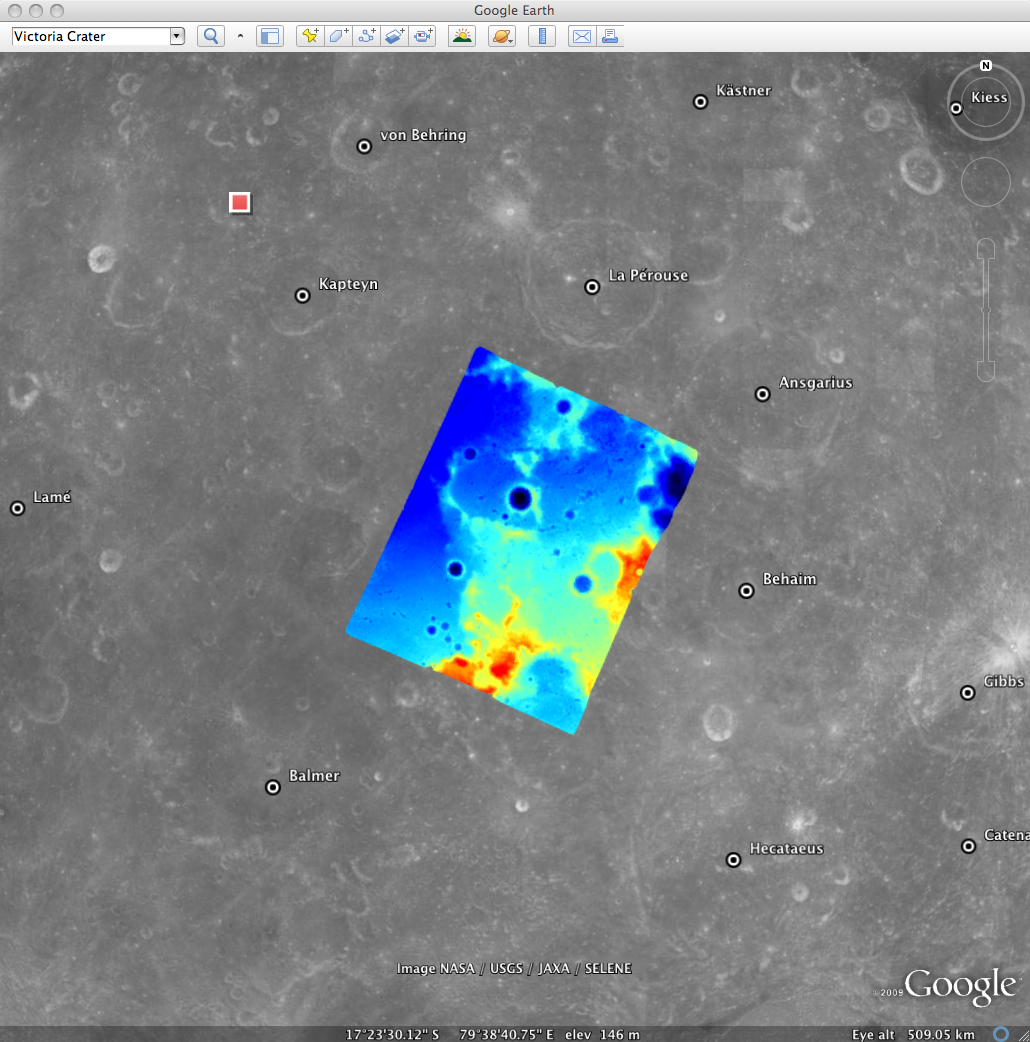
\includegraphics[width=3in]{images/examples/metric/metric_ge_example.png}}
\caption{Example output possible with Apollo Metric frames AS15-M-2380 and AS15-M-2381.}
\label{fig:metric_example}
\end{figure}

\subsubsection*{Commands}

\begin{verbatim}
    % Process tif files with not yet released commands %
    reduce from=AS15-M-2380.cub to=sub4-AS15-M-2380.cub sscale=4 lscale=4
    reduce from=AS15-M-2381.cub to=sub4-AS15-M-2381.cub sscale=4 lscale=4
    spiceinit from=sub4-AS15-M-2380.cub
    spiceinit from=sub4-AS15-M-2381.cub
    ipfind --max 10000 sub4*.cub
    ipmatch -i 50 -r homography sub4*.cub
    mkdir result
    stereo sub4-AS15-M-2380.cub sub4-AS15-M-2381.cub result/output
\end{verbatim}

\subsubsection*{Stereo Default}

\begin{verbatim}
    ### PREPROCESSING

    DO_INTERESTPOINT_ALIGNMENT 1
    INTERESTPOINT_ALIGNMENT_SUBSAMPLING 0
    DO_EPIPOLAR_ALIGNMENT 0

    FORCE_USE_ENTIRE_RANGE 1
    DO_INDIVIDUAL_NORMALIZATION 0

    PREPROCESSING_FILTER_MODE 3

    SLOG_KERNEL_WIDTH 1.5

    ### CORRELATION

    COST_MODE 2
    COST_BLUR 25

    H_KERNEL 35
    V_KERNEL 35

    H_CORR_MIN -250
    H_CORR_MAX 250
    V_CORR_MIN -70
    V_CORR_MAX 100

    SUBPIXEL_MODE 2

    SUBPIXEL_H_KERNEL 25
    SUBPIXEL_V_KERNEL 25

    # Hidden advanced function
    CORRSCORE_REJECTION_THRESHOLD 1.4

    ### FILTERING

    FILL_HOLES 1

    RM_H_HALF_KERN 5
    RM_V_HALF_KERN 5
    RM_MIN_MATCHES 60 # Units = percent
    RM_THRESHOLD 3
    RM_CLEANUP_PASSES 1

    ### DOTCLOUD

    NEAR_UNIVERSE_RADIUS 0.0
    FAR_UNIVERSE_RADIUS 0.0
\end{verbatim}


\section{MESSENGER MDIS}

These results are a proof of concept showing off the strength of
building the Stereo Pipeline on top of ISIS. Support for
processing MDIS stereo pairs was not a goal during our design of the
software, but the fact that an MDIS camera model exists in ISIS means
that it too can be processed by the Stereo Pipeline.

For future mappers, we suggest checking out Mercury Flyby 3 data which
was not available at the time of this writing. Flyby 3 and Flyby 2
seem to have covered some of the same terrain with the narrow angle
camera.

\subsection{Wide Angle on flyby 2}

In most flyby imagery it is very hard to find good stereo pairs. This
pair was taken from a single flyby just seconds apart. Note also that
this pair is taken from different wave lengths \emph{(The letter at
  the end of the file designates the current filter being used on the
  wide angle camera)}. Unfortunately there is not enough of a
perspective change here to make anything other than the spherical
surface, but that alone is still an interesting result nonetheless.

\subsubsection*{Screenshot}

\begin{figure}[h!]
  \begin{center}
  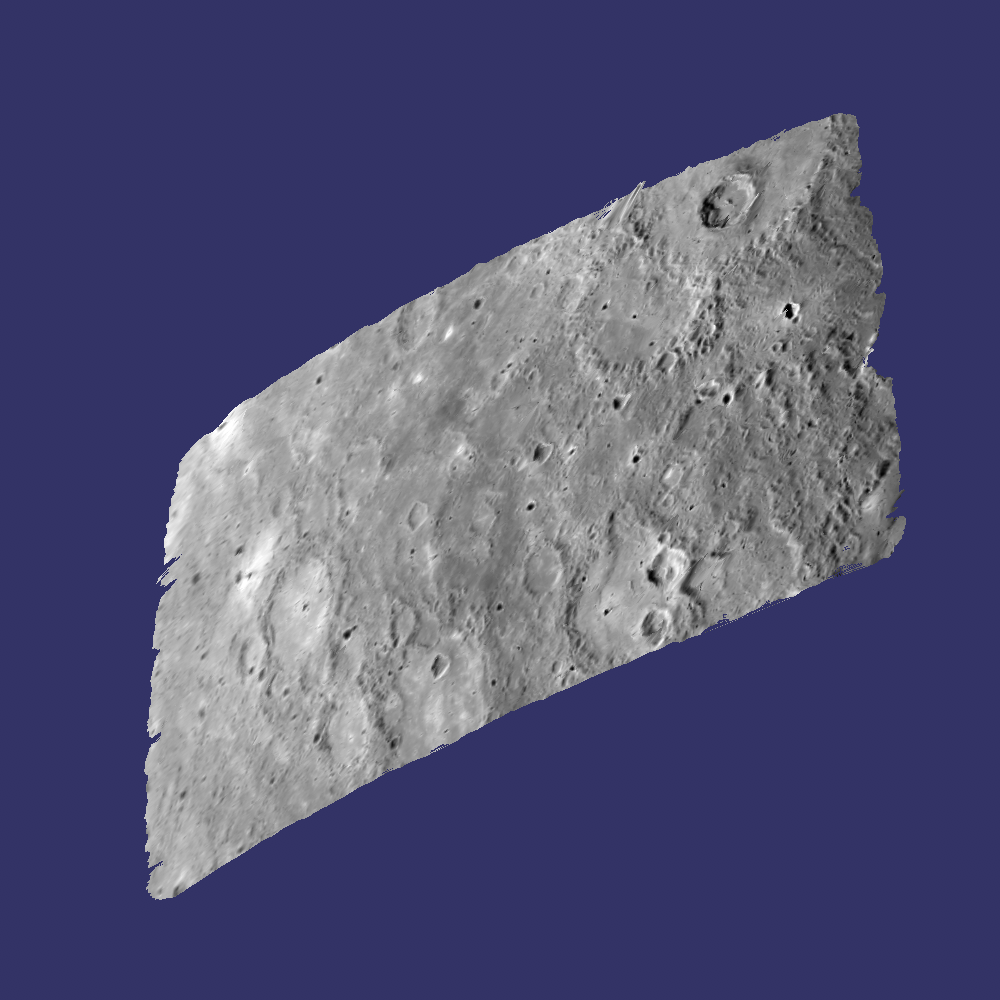
\includegraphics[width=5in]{images/examples/mdis/mdis_wide_example.png}
  \end{center}
  \caption{ A rough attempt at stereo reconstruction from MDIS imagery. }
  \label{fig:mdis_attempt}
\end{figure}

\subsubsection*{Commands}

\begin{verbatim}
    mdis2isis from=EW0108825359A.IMG to=EW0108825359A.cub
    mdis2isis from=EW0108825379C.IMG to=EW0108825379C.cub
    spiceinit from=EW0108825359A.cub
    spiceinit from=EW0108825359C.cub
    ipfind --max 10000 *.cub
    ipmatch -i 10 -r homography *.cub
    mkdir result
    stereo EW0108825359A.cub EW0108825379C.cub stereo/output
\end{verbatim}

\subsubsection*{Stereo Default}

\begin{verbatim}
    ### PREPROCESSING

    DO_INTERESTPOINT_ALIGNMENT 1
    INTERESTPOINT_ALIGNMENT_SUBSAMPLING 0
    DO_EPIPOLAR_ALIGNMENT 0

    FORCE_USE_ENTIRE_RANGE 0
    DO_INDIVIDUAL_NORMALIZATION 1

    PREPROCESSING_FILTER_MODE 2

    SLOG_KERNEL_WIDTH 1.5

    ### CORRELATION

    COST_BLUR 5
    COST_MODE 0

    H_KERNEL 25
    V_KERNEL 25

    H_CORR_MIN -10
    H_CORR_MAX 10
    V_CORR_MIN -2
    V_CORR_MAX 2

    SUBPIXEL_MODE 2

    SUBPIXEL_H_KERNEL 19
    SUBPIXEL_V_KERNEL 19

    ### FILTERING

    FILL_HOLES 1

    RM_H_HALF_KERN 5
    RM_V_HALF_KERN 5
    RM_MIN_MATCHES 60 # Units = percent
    RM_THRESHOLD 3
    RM_CLEANUP_PASSES 1

    ### DOTCLOUD

    NEAR_UNIVERSE_RADIUS 0.0
    FAR_UNIVERSE_RADIUS 0.0

\end{verbatim}

\section{Cassini ISS NAC}

This is a proof of concept showing the strength of building the Stereo
Pipeline on top of ISIS.  Support for processing ISS NAC stereo pairs
was not a goal during our design of the software, but the fact that a
camera model exists in ISIS means that it too can be processed by the
Stereo Pipeline.

Identifying stereo pairs from satellites that do not orbit their
target is a challenge. We have found that one usually has to settle
with images that are not ideal: different lighting, little perspective
change, and little or no stereo parallax. So far we have had little
succes with Cassini's difficult data, but nonetheless we provide this
example as a potential starting point.

\subsection{Rhea}

Rhea is the second largest moon of Saturn and is roughly 1/3rd the
size of our own Moon. This example show, at the top right of both
images,a gaint impact basin named Tirawa that is 220 miles across. The
bright white area south of Tirawa is ejecta from a new crater.  The
lack of texture in this area poses a challenge for our correlator. The
results are just barely useful: the Tirawa impact can barely be made
out in the 3D data while the new crater and ejecta become only noise.

\subsubsection*{Screenshot}

\begin{figure}[p]
\centering
  \subfigure[{\tt Original Left Image}]{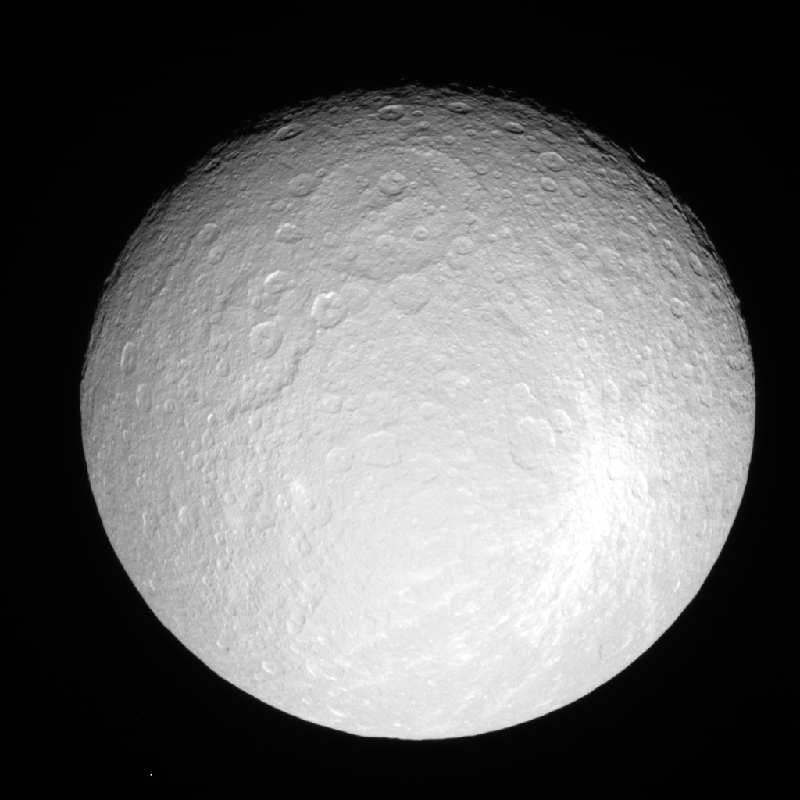
\includegraphics[width=3in]{images/examples/cassini/cassini_rhea_L.png}}
  \hfil
  \subfigure[{\tt Original Right Image}]{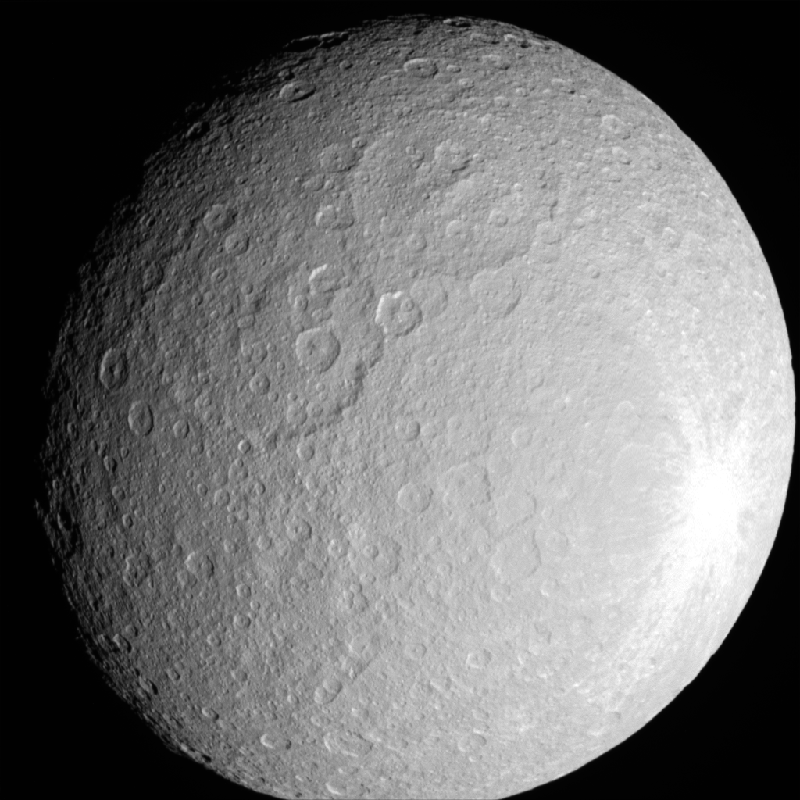
\includegraphics[width=3in]{images/examples/cassini/cassini_rhea_R.png}}
  \\
  \subfigure[{\tt Map Projected Left}]{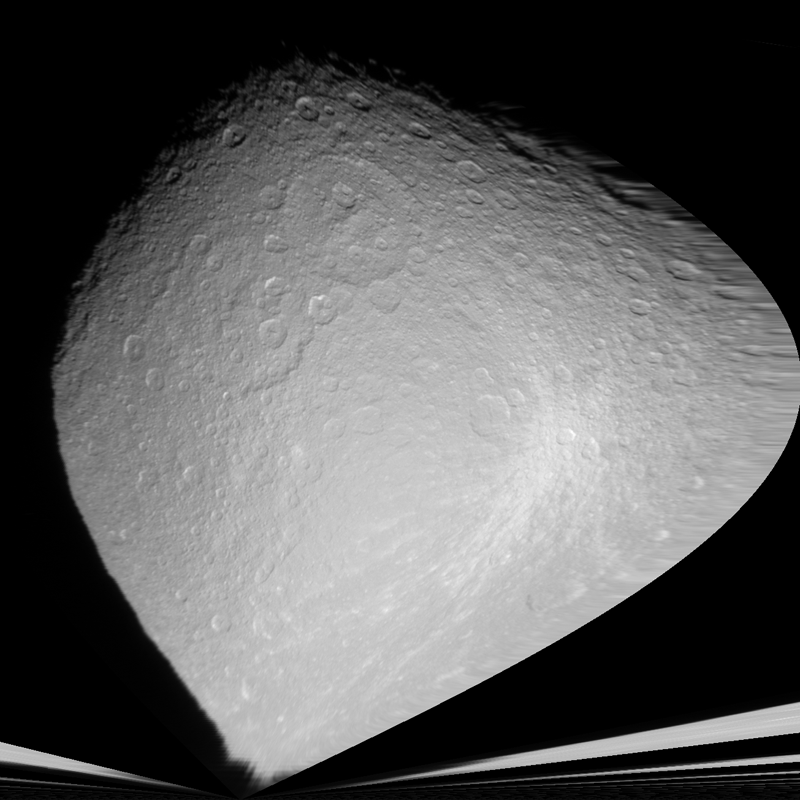
\includegraphics[width=3in]{images/examples/cassini/cassini_rhea_map.png}}
  \hfil
  \subfigure[{\tt 3D Rendering}]{\includegraphics[width=3in]{images/examples/cassini/cassini_rhea.png}}
\caption{Example output of what is possible with Cassini's ISS NAC}
\label{fig:cassini-exampe}
\end{figure}

\subsubsection*{Commands}

\begin{verbatim}
    % Download N1511700120_1.IMG and W1567133629_1.IMG
    ciss2isis f=N1511700120_1.IMG t=N1511700120_1.cub
    ciss2isis f=W1567133629_1.IMG t=W1567133629_1.cub
    cisscal from=N1511700120_1.cub to=N1511700120_1.lev1.cub
    cisscal from=W1567133629_1.cub to=W1567133629_1.lev1.cub
    fillgap from=W1567133629_1.lev1.cub to=W1567133629_1.fill.cub %Only one image
                                                                  %exhibits the problem
    cubenorm from=N1511700120_1.lev1.cub to=N1511700120_1.norm.cub
    cubenorm from=W1567133629_1.fill.cub to=W1567133629_1.norm.cub
    cam2map from=N1511700120_1.norm.cub to=N1511700120_1.map.cub
    cam2map from=W1567133629_1.norm.cub map=N1511700120_1.map.cub ...
            to=W1567133629_1.map.cub matchmap=true;
    ls *.map.cub > fromlist
    ls N*.map.cub > holdlist
    equalizer fromlist=fromlist holdlist=holdlist
    mkdir result
    stereo N1511700120_1.map.equ.cub W1567133629_1.map.equ.cub result/rhea
\end{verbatim}

\subsubsection*{Stereo Default}

\begin{verbatim}
    ### PREPROCESSING

    DO_INTERESTPOINT_ALIGNMENT 0
    INTERESTPOINT_ALIGNMENT_SUBSAMPLING 0
    DO_EPIPOLAR_ALIGNMENT 0

    FORCE_USE_ENTIRE_RANGE 1
    DO_INDIVIDUAL_NORMALIZATION 1

    PREPROCESSING_FILTER_MODE 2

    SLOG_KERNEL_WIDTH 1.5

    ### CORRELATION

    COST_MODE 2
    COST_BLUR 11

    H_KERNEL 25
    V_KERNEL 25

    H_CORR_MIN -55
    H_CORR_MAX -5
    V_CORR_MIN -2
    V_CORR_MAX 10

    SUBPIXEL_MODE 3 # Experimental Subpixel Mode

    SUBPIXEL_H_KERNEL 21
    SUBPIXEL_V_KERNEL 21

    ### FILTERING

    FILL_HOLES 1

    RM_H_HALF_KERN 5
    RM_V_HALF_KERN 5
    RM_MIN_MATCHES 60 # Units = percent
    RM_THRESHOLD 3
    RM_CLEANUP_PASSES 1

    ### DOTCLOUD

    NEAR_UNIVERSE_RADIUS 0.0
    FAR_UNIVERSE_RADIUS 0.0
\end{verbatim}


%\part{Additional Toolkits}
%\chapter{Control Network Toolkit}
\label{ch:controlnettk}

This chapter covers the first additional boost of tools for \ac{ASP}!
Control Networks are a data structure that at their core contain image
features that can be tracked in multiple images. Since these features
can be tracked in multiple images, they can be triangulated and
represent a 3D location. This control network can then be used in
processes such as Bundle Adjustment using tools like
\texttt{isis\_adjust} and \texttt{jigsaw}.

\emph{Warning: This toolkit is not finished but this documentation
  hopes to allow some use in its early state.}

The method of developing a control network with \ac{VW} and \ac{ASP}
is that we try to track as many 'natural' features and then reduce
into a control network. This is done in a 6 step process.

\begin{itemize}
\item Detect features using a second order filter \emph{(LoG)}.
\item Describe these features by their surroundings with a tag.
\item Match tags of interest points between images.
\item Filter these matches for error using RANSAC.
\item Reduce matches further for ease of processing and also to assure uniform distribution.
\item Collect all pair-wise matches and write as Control Network.
\end{itemize}

I'm going to provide an example of how to use this software with
Apollo Metric images. Hopefully you can follow along with whatever
imagery you happen to have around. Note in the example below we use a
lot of calls to \texttt{xargs}. That command is helpful for spawning
multiple processes to work on a pool of jobs. The argument \emph{\-P 10}
states that at most it should have 10 processes running
simultaneously. Lower that value to the number of cores available on
your system.

We are going to start out first by gathering interest points \emph{(or
  features)} and this is accomplished with a tool called
\texttt{ipfind}. This handy tool is provided by \ac{VW} and is not
built against ISIS. This means it can only read cube files through a
library called GDAL. To make sure cubes files can be read correctly by
GDAL and thus ipfind, we'll have to convert our input imagery to
something more reliable like TIFFs.

\begin{verbatim}
    ISIS 3> isis2std from=INPUT to=OUTPUT.tif format=TIFF
\end{verbatim}

I don't like to call isis2std on every file myself. Here's the
commands I use to do this in parallel.

\begin{verbatim}
    ISIS 3> echo *.cub | xargs -n1 echo | awk -F "." '{print $1}' |
              xargs -n1 -P 10 -I {} isis2std from={}.cub to={}.tif format=TIFF
\end{verbatim}

The directory should now be filled with TIFF format doppelgangers. We
are ready to perform \texttt{ipfind} which will detect features and
describe them in one go. The results of each operation will be saved
in a \texttt{.vwip} file which will later be read during
matching. There are many algorithms that \texttt{ipfind} can use for
detection and description but the defaults of OBALoG and SGrad should
do fine for most situations. Also note that \texttt{ipfind} has a
debug flag '-d' which can be used to output debug images that show the
location of all detected features.

\begin{verbatim}
  > echo *.tif | xargs -n1 -P 10 ipfind --max 10000
\end{verbatim}

Notice the options \emph{\-\-max 10000} used for the \texttt{ipfind}
example. This is to limit the number of detected interest points so
that the next step doesn't take too long.

Matching is calculated pairwise. There are many ways to do this, but
the simplists is just a brute force permutation of all possible
combinations. Here's how:

\begin{verbatim}
  > pairlist_all.py *.tif | xargs -n2 -P 10 ipmatch -r homography
\end{verbatim}

Alternatively we could just match between images that happen to be
sequential by name.

\begin{verbatim}
  > pairlist_seq.py *.tif | xargs -n2 -P 10 ipmatch -r homography
\end{verbatim}

Though for large datasets it doesn't seem approriate to compare all
images to each other as the physically don't see each other in
anyway. A good way of reducing the matches is by deciding to only
calculate matches between images that are separated by no more than a
few degrees. This is what \texttt{pairlist\_degree.py} can
do. Internally it calls \texttt{camrange} and this can take a
while. I'd recommend saving the output to a file before sending out to
ipmatch.

\begin{verbatim}
    ISIS 3> pairlist_degree.py *cub -a 10 -iext tif > pairs_to_process.lst
    ISIS 3> cat pairs_to_process.lst |
              xargs -n2 -P 10 ipmatch -r homography
\end{verbatim}

If you've been reading the output from ipmatch, you may have noticed
that some pair-wise matches might have more than a 100 matches! This
is probably overkill for some cases and could potentially choke an
application further down the process. Also at this point, our interest
points could be located anywhere. The worst case is that all matched
features have managed to clump around interesting objects like a
sparkly crater or a sharp cut rill. We can't enforce that the matched
features are evenly placed, but we can trim them down to be somewhat
even.

Enter stage left, \texttt{reduce\_match}. This utility will thin down
the matches so that they are evenly distributed. You specify the
minimum and maximum amount of matches that can exist for a pair of
images. Setting the maximum trims down excessive matches. The minimum
however will actually delete match files that have to few matches. The
filtering function RANSAC that is used to remove outliers does not
have a graceful failure. When that algorithm fails it will return all
outliers but usually with the minimum number of matches to solve for
its fitting functor. Using a homography fitting functor means 8
matches. We'll go ahead and delete anything 10 and under.

\begin{verbatim}
  > echo *.match | xargs -n1 -P 10 reduce_match --min 10 --max 100
\end{verbatim}

Finally we are ready to collect all pairwise matches into a single
control network. From the same directory that houses all match files
and cube files, we will call the command
\texttt{cnet\_build}. Assuming we want to build an ISIS style control
network, here's how to perform the last step.

\begin{verbatim}
  > cnet_build *.cub -t isis -o asp_control
\end{verbatim}

Let's go ahead and see how the results turned out in qnet!

\begin{verbatim}
    ISIS 3> echo *.cub | xargs -n1 echo > cube.lst
    ISIS 3> qnet
\end{verbatim}

Inside qnet you'll want to click 'open'. On the first dialog you'll
pick out the \emph{cube.lst} file we just created. On the second, we
pick our created control network \emph{asp\_control.net}.

\begin{center}
\includegraphics[height=3.7in]{images/cnettk_qnet_screen.png}
\end{center}

Occasionally you might find yourself not quite satisfied with results
of Control Network Toolkit. Don't worry, we won't take it
personally. However there are still some options available to you. You
could do manual tie point additions with \texttt{qnet}. However, this
can be a slow and scary process if you need to load up the entire
control network. Instead you can just load up the problem images and
do manual tie pointing. Then afterwards you could merge this smaller
control network with the large control network you created with
\texttt{cnet\_merge}.

\begin{verbatim}
  > cnet_merge large.cnet small.net -o larger.cnet
\end{verbatim}

The above command will create an even larger control network which
contains both \emph{large.cnet} and \emph{small.net}. This is helpful
for filling in those spots where the automatic control network failed
to work.

%\include{Photometrytk}

\part{Appendices}
\appendix
\chapter{Tools}

This chapter provides a overview of the various tools that are
provided as part of the Ames Stereo Pipeline, and a summary of their
command line options.

\section{stereo}
\label{stereo}

The \texttt{stereo} program is the primary tool of the Ames Stereo
Pipeline. It takes a stereo pair of images that overlap and creates an
output point cloud image that can be processed into a visualizable mesh
or a DEM using \texttt{point2mesh} (section \ref{point2mesh}) and
\texttt{point2dem} (section \ref{point2dem}), respectively.

\medskip

Usage:
\begin{verbatim}
  ISIS 3> stereo [options] <images> [<cameras>] output_file_prefix
\end{verbatim}

Example (for ISIS):
\begin{verbatim}
  stereo file1.cub file2.cub results/run
\end{verbatim}
For ISIS, a .cub file has both image and camera information, as such
no separate camera files are specified.

Example (for Digital Globe Earth images):
\begin{verbatim}
  stereo file1.tif file2.tif file1.xml file2.xml results/run
\end{verbatim}

Multiple input images are also supported (section \ref{multiview}).

This tool is is primarily designed to process USGS ISIS \texttt{.cub}
files and Digital Globe data. However, Stereo Pipeline
does have the capability to process other types of stereo image pairs
(e.g., image files with a CAHVOR camera model from the NASA MER
rovers). If you would like to experiment with these features, please
contact us for more information.

The \texttt{\textit{output\_file\_prefix}} is prepended to all
output data files.  For example, setting \texttt{\textit{output\_file\_prefix}}
to `\texttt{out}' will yield files with names like \texttt{out-L.tif}
and \texttt{out-PC.tif}.  To keep the Stereo Pipeline results organized
in sub-directories, we recommend using an output prefix like
`\texttt{results-10-12-09/out}' for \texttt{\textit{output\_file\_prefix}}.  The
\texttt{stereo} program will create a directory called
\texttt{results-10-12-09/} and place files named \texttt{out-L.tif},
\texttt{out-PC.tif}, etc. in that directory.

\begin{longtable}{|l|p{7.5cm}|}
\caption{Command-line options for stereo}
\label{tbl:stereo}
\endfirsthead
\endhead
\endfoot
\endlastfoot
\hline
Option & Description \\ \hline \hline
\texttt{-\/-help|-h} & Display the help message\\ \hline
\texttt{-\/-session-type|-t pinhole|isis|dg|rpc|spot5|aster|pinholemappinhole|isismapisis|dgmaprpc|rpcmaprpc|astermaprpc} & Select the stereo session type to use for processing. Usually the program can select this automatically by the file extension.\\ \hline
\texttt{-\/-stereo-file|-s \textit{filename(=./stereo.default)}} & Define the stereo.default file to use.\\ \hline
\texttt{-\/-entry-point|-e integer(=0 to 4)} & Stereo Pipeline entry
point (start at this stage). \\ \hline
\texttt{-\/-stop-point|-e integer(=1 to 5)} & Stereo Pipeline stop point (stop at the stage {\it right before} this value). \\ \hline
\texttt{-\/-corr-seed-mode integer(=0 to 3)} & Correlation seed strategy (section \ref{corr_section}). \\ \hline
\texttt{-\/-threads \textit{integer(=0)}} & Set the number of threads to use. 0 means use as many threads as there are cores.\\ \hline
\texttt{-\/-no-bigtiff} & Tell GDAL to not create bigtiffs.\\ \hline
\texttt{-\/-tif-compress None|LZW|Deflate|Packbits} & TIFF compression method.\\ \hline
\end{longtable}

More information about additional options that can be passed to \texttt{stereo}
via the command line or via the \texttt{stereo.default} configuration file can be
found in Appendix \ref{ch:stereodefault} on page
\pageref{ch:stereodefault}.  \texttt{stereo} creates a set
of intermediate files, they are described in Appendix
\ref{chapter:outputfiles} on page \pageref{chapter:outputfiles}.

\subsection{Entry Points}
\label{entrypoints}

The \texttt{stereo -e \textit{number}} option can be used to restart
a {\tt stereo} job partway through the stereo correlation process.
Restarting can be useful when debugging while iterating on {\tt
stereo.default} settings.

Stage 0 (Preprocessing) normalizes the two images and aligns them
by locating interest points and matching them in both images. The
program is designed to reject outlying interest points.  This stage
writes out the pre-aligned images and the image masks.

Stage 1 (Disparity Map Initialization) performs pyramid correlation and builds a rough disparity map that is used to seed the sub-pixel refinement phase.

Stage 2 (Sub-pixel Refinement) performs sub-pixel correlation that
refines the disparity map.

Stage 3 (Outlier Rejection and Hole Filling) performs filtering of the
disparity map and (optionally) fills in holes using an inpainting
algorithm.  This phase also creates a ``good pixel'' map.

Stage 4 (Triangulation) generates a 3D point cloud from the disparity
map.

\subsection{Decomposition of Stereo}
\label{stereo_dec}

The \texttt{stereo}
executable is a python script that makes calls to separate
C++ executables for each entry point.

Stage 0 (Preprocessing) calls \texttt{stereo\_pprc}. Multi-threaded.

Stage 1 (Disparity Map Initialization) calls
\texttt{stereo\_corr}. Multi-threaded.

Stage 2 (Sub-pixel Refinement) class \texttt{stereo\_rfne}. Multi-threaded.

Stage 3 (Outlier Rejection and Hole Filling) calls
\texttt{stereo\_fltr}. Multi-threaded.

Stage 4 (Triangulation) calls \texttt{stereo\_tri}. Multi-threaded,
except for ISIS input data.

All of the sub-programs have the same interface as
\texttt{stereo}. Users processing a large number of stereo pairs on a
cluster may find it advantageous to call these executables in their own
manner. An example would be to run stages 0-3 in order for each stereo
pair. Then run several sessions of \texttt{stereo\_tri} since it is
single-threaded for ISIS.

It is important to note that each of the C++ stereo executables invoked
by \texttt{stereo} have their own command-line options. Those options
can be passed to \texttt{stereo} which will in turn pass them to the
appropriate executable. By invoking each executable with no options, it
will display the list of options it accepts.

As explained in more detail
in section \ref{perform-stereo}, each such option has the same syntax as
used in \texttt{stereo.default}, while being prepended by a double hyphen
(\texttt{-\/-}).  A command line option takes precedence over the same
option specified in \texttt{stereo.default}. Chapter \ref{ch:stereodefault}
documents all options for the individual sub-programs.

Note that the stereo tools operate only on single channel (grayscale) images.
If you need to run stereo on multi-channel images you must first convert them
to grayscale or extract a single channel to operate on.

\section{stereo\_gui}
\label{stereo_gui}

The \texttt{stereo\_gui} program is a GUI frontend to \texttt{stereo},
and has the same command-line options. It can display the input images
side-by-side (and in other ways, as detailed later). One can zoom in by
dragging the mouse from upper-left to lower-right, and zoom out via the
reverse motion.

By pressing the \texttt{Control} key while dragging the mouse, regions
can be selected in the input images, and then stereo can be run on these
regions from the menu via Run$\rightarrow$Stereo. The \texttt{stereo}
command that is invoked (with appropriately populated parameter values
for \texttt{-\/-left-image-crop-win} and \texttt{-\/-right-image-crop-win}
for the selected regions) will
be displayed on screen, and can be re-run on a more powerful
machine/cluster without GUI access.

Additional navigation options are using the mouse wheel or the +/- keys to
zoom, and the arrow keys to pan (one should first click to bring into
focus the desired image before using any keys).

\begin{figure}[h!]
\begin{center}
\includegraphics[width=5in]{images/stereo_gui.jpg}
\caption[asp\_gui]{An illustration of stereo\_gui. The \texttt{stereo} command
will be run on the regions selected by red rectangles.}
\label{asp_gui_fig}
\end{center}
\end{figure}

Usage:
\begin{verbatim}
  ISIS 3> stereo_gui [options] <images> [<cameras>] output_file_prefix
\end{verbatim}

\subsection{Use as an Image Viewer}

This program can be also used as a general-purpose image viewer, case in
which no stereo options or camera information is necessary.  It can
display arbitrarily large images with integer, floating-point, or RGB
pixels, including ISIS .cub files and DEMs. It handles large images by
building on disk pyramids of increasingly coarser subsampled images and
displaying the subsampled versions that are appropriate for the current
level of zoom.

The images can be shown either side-by-side, as tiles on a grid (using
\texttt{-\/-grid-cols integer}), or on top of each other (using
\texttt{-\/-single-window}), with a dialog to choose among them.  In the
last usage scenario, the option \texttt{-\/-use-georef} will overlay the
images correctly if georeference information is present.  It is possible
to switch among these modes once the GUI has been open, from the GUI
View menu. When the images are shown side-by-side, the GUI can zoom
in all images to the same region, for easier comparison among them.

\texttt{stereo\_gui} can show hillshaded DEMs, either via the
\texttt{-\/-hillshade} option, or by choosing from the GUI View menu the
\texttt{Hillshaded images} option.

This program can also display the output of the ASP \texttt{colormap}
tool (section \ref{sec:colormap}).

When clicking on a pixel, the pixel indices and value will be printed on screen.
When selecting a region by pressing the \texttt{Control} key while dragging the mouse, 
its bounds will be displayed on screen. If the image is geo-referenced,
the extent of the region in projected coordinates and in the longitude-latitude domain 
will be shown as well. 

The program can also save a screenshot to disk in the BMP or XPM format. 

\subsection{Other Functionality}

\subsubsection{View/create/delete/save interest point matches}

\texttt{stereo\_gui} can be used to view interest point matches
(\texttt{*.match} files), such as generated by \texttt{bundle\_adjust}
and \texttt{stereo}. It can also manually create and delete
matches (useful in situations when automatic interest point matching is
unreliable due to large changes in illumination).

The match file to load can be specified via \texttt{-\/-match-file}.  It
may also be auto-detected if \texttt{stereo\_gui} was invoked like
\texttt{stereo}, with an output prefix (auto-detection works only when
images are not map-projected and alignment is homography or affine
epipolar).

\subsubsection{Create GCP}
\label{bagcp}

\texttt{stereo\_gui} can be used to create
ground control point (GCP) files for \texttt{bundle\_adjust}. It is
assumed that the user has two or more images and corresponding cameras
that need adjustment. It is also assumed that there exists an additional
reference image, possible from another source, that is georeferenced,
and a reference DEM from which one can infer xyz coordinates. All these
images, but not the cameras or the reference DEM, should be loaded in the
GUI, with the reference georeferenced image being the last. For each
output ground control point, an interest point must be picked manually
in each of the images. When finished, use the "IP matches"->"Write GCP
file" menu item to generate a ground control point file containing the
selected points.  You will be prompted for the reference DEM and for the
desired output file name. The last image, that is the reference, is only
used to find the positions on the ground, which in turn are used to find
the heights for the GCPs from the DEM. The selected interest points from
the reference image are not saved to the GCP file.

\subsubsection{Shadow threshold}
\texttt{stereo\_gui} can be used to find the shadow threshold for each
of a given set of images (useful for shape-from-shading (chapter \ref{ch:sfs}).
This can be done by turning on from the menu
the \texttt{Shadow threshold detection} mode, and then clicking on
pixels in the shadow. The largest of the chosen pixel values will be set
to the shadow threshold for each image and printed to the screen. To see
the images with the pixels below the shadow threshold highlighted,
select from the menu the \texttt{View shadow-thresholded images} option.

\clearpage
Listed below are the options specific to \texttt{stereo\_gui}. It will accept
all other \texttt{stereo} options as well.

\begin{longtable}{|l|p{7.5cm}|}
\caption{Command-line options for stereo\_gui}
\label{tbl:stereogui}
\endfirsthead
\endhead
\endfoot
\endlastfoot
\hline
Option & Description \\ \hline \hline
\texttt{-h | -\/-help } & Display this help message.\\ \hline
\texttt{-\/-grid-cols arg} & Display images as tiles on a grid with this many columns. Default: Use one row.\\ \hline
\texttt{-\/-window-size arg (=1200 800)} & The width and height of the GUI window in pixels.\\ \hline
\texttt{-w | -\/-single-window } & Show all images in the same window (with a dialog to choose among them) rather than next to each other.\\ \hline
\texttt{-\/-use-georef} & Plot the images in the projected coordinate system given by image georeferences.\\ \hline
\texttt{-\/-hillshade} & Interpret the input images as DEMs and hillshade them.\\ \hline
\texttt{-\/-hillshade-azimuth} & The azimuth value when showing hillshaded images.\\ \hline
\texttt{-\/-hillshade-elevation} & The elevation value when showing hillshaded images.\\ \hline

\texttt{-\/-view-matches} & Locate and display the interest point matches.\\ \hline
\texttt{-\/-match-file} & Display this match file instead of looking one up based on existing conventions (implies \texttt{-\/-view-matches}). \\ \hline
\texttt{-\/-gcp-file} & Display the GCP pixel coordinates for this GCP file (implies \texttt{-\/-view-matches}). \\ \hline
\texttt{-\/-delete-temporary-files-on-exit} & Delete any subsampled and other files created by the GUI when exiting.\\ \hline
\texttt{-\/-create-image-pyramids-only} & Without starting the GUI, build multi-resolution pyramids for the inputs, to be able to load them fast later.\\ \hline
\end{longtable}

\section{parallel\_stereo}
\label{parallel}

The \texttt{parallel\_stereo} program is a modification of
\texttt{stereo} designed to distribute the stereo processing over
multiple computing nodes. It uses GNU Parallel to manage the jobs, a tool which
is distributed along with Stereo Pipeline. It expects that all nodes
can connect to each other using ssh without password. \texttt{parallel\_stereo}
can also be useful when processing extraterrestrial data on a single computer.
This is because ISIS camera models are restricted to a single thread, but
\texttt{parallel\_stereo} can run multiple processes in parallel to reduce
computation times.

At the simplest, \texttt{parallel\_stereo} can be invoked exactly like \texttt{stereo},
with the addition of the list of nodes to use (if using multiple nodes).

\begin{verbatim}
  parallel_stereo --nodes-list machines.txt <other stereo options>
\end{verbatim}

It will create the same output files as \texttt{stereo}. (Internally
some of them will be GDAL VRT files, that is, virtual mosaics of files created
by individual processes; ASP and GDAL tools are able to use these
virtual files in the same way as regular binary TIF files.)

If your jobs are launched on a cluster or supercomputer, the name of the
file containing the list of nodes may exist as an environmental
variable. For example, on NASA's Pleiades Supercomputer, which uses the
Portable Batch System (PBS), the list of nodes can be retrieved as
\$PBS\_NODEFILE.

It is important to note that when invoking this tool only stages 1, 2,
and 4 of stereo (section \ref{stereo_dec}) are spread over multiple
machines, with stages 0 and 3 using just one node, as they require
global knowledge of the data. In addition, not all stages of stereo
benefit equally from parallelization. Most likely to gain are stages 1
and 2 (correlation and refinement) which are the most computationally
expensive.

For these reasons, while \texttt{parallel\_stereo} can be called to do
all stages of stereo generation from start to finish in one command, it
may be more resource-efficient to invoke it using a single node for
stages 0 and 3, many nodes for stages 1 and 2, and just a handful of
nodes for stage 4 (triangulation). For example, to invoke the tool
only for stage 2, one uses the options:

\begin{verbatim}
  --entry-point 2 --stop-point 3
\end{verbatim}

By default, stages 1, 2, and 4 of \texttt{parallel\_stereo} use
as many processes as there are cores on each node, and one thread per process.
These can be customized as shown below.

\begin{longtable}{|l|p{7.5cm}|}
\caption{Command-line options for parallel\_stereo}
\label{tbl:parallelstereo}
\endfirsthead
\endhead
\endfoot
\endlastfoot
\hline
Options & Description \\ \hline \hline
\texttt{-\/-help|-h} & Display the help message.\\ \hline
\texttt{-\/-nodes-list \textit{filename} } & The list of computing nodes,
one per line. If not provided, run on the local machine. \\ \hline
\texttt{-\/-entry-point|-e integer(=0 to 4)} & Stereo Pipeline entry
point (start at this stage). \\ \hline
\texttt{-\/-stop-point|-e integer(=1 to 5)} & Stereo Pipeline stop point
(stop at the stage {\it right before} this value). \\ \hline
\texttt{-\/-corr-seed-mode integer(=0 to 3)} & Correlation seed strategy
(section \ref{corr_section}). \\ \hline
\texttt{-\/-sparse-disp-options \textit{string} } & Options to pass directly
to sparse\_disp (section \ref{sparse-disp}). \\ \hline
\texttt{-\/-verbose } & Display the commands being executed. \\ \hline
\texttt{-\/-job-size-w \textit{integer(=2048)}} & Pixel width of input
image tile for a single process. \\ \hline
\texttt{-\/-job-size-h \textit{integer(=2048)}} & Pixel height of input
image tile for a single process. \\ \hline
\texttt{-\/-processes \textit{integer}} & The number of processes to use per node. \\ \hline
\texttt{-\/-threads-multiprocess \textit{integer}} & The number of threads to use per process.\\ \hline
\texttt{-\/-threads-singleprocess \textit{integer}} & The number of threads to use when running a single process (for pre-processing and filtering).\\ \hline
\end{longtable}

\newpage
\section{bundle\_adjust}
\label{bundleadjust}

The \texttt{bundle\_adjust} program performs bundle adjustment on a
given set of images and cameras. An introduction to bundle adjustment
can be found in chapter \ref{ch:bundle_adjustment}, with an example of
how to use this program in section \ref{baasp}.

This tool can use several algorithms for bundle adjustment. The default is
to use Google's Ceres Solver (\url{http://ceres-solver.org/}).

Usage:
\begin{verbatim}
  bundle_adjust <images> <cameras> <optional ground control points> \
    -o <output prefix> [options]
\end{verbatim}

Example (for ISIS):
\begin{verbatim}
  bundle_adjust file1.cub file2.cub file3.cub -o results/run
\end{verbatim}

Example (for Digital Globe Earth data, using ground control points):
\begin{verbatim}
  bundle_adjust file1.tif file2.tif file1.xml file2.xml gcp_file.gcp \
    --datum WGS_1984 -o results/run
\end{verbatim}

Example (for generic pinhole camera data, using estimated camera positions):
\begin{verbatim}
  bundle_adjust file1.JPG file2.JPG file1.tsai file2.tsai -o results/out \
     -t pinhole --local-pinhole --datum WGS_1984 --camera-positions nav_data.csv \
     --csv-format "1:file 6:lat 7:lon 9:height_above_datum"
\end{verbatim}

The \texttt{stereo} program can then be told to use the adjusted cameras
via the option \texttt{-\/-bundle-adjust-prefix}.

\begin{longtable}{|l|p{7.5cm}|}
\caption{Command-line options for bundle\_adjust}
\label{tbl:bundleadjust}
\endfirsthead
\endhead
\endfoot
\endlastfoot
\hline
Option & Description \\ \hline \hline
\texttt{-\/-help|-h} & Display the help message. \\ \hline

\texttt{-\/-output-prefix|-o \textit{filename}} & Prefix for output filenames. \\ \hline

\texttt{-\/-bundle-adjuster \textit{string [default: Ceres]}} & Choose a solver from:
Ceres, RobustSparse, RobustRef, Sparse, Ref. \\ \hline

\texttt{-\/-cost-function \textit{string [default: Cauchy]}} & Choose a cost function
from: Cauchy, PseudoHuber, Huber, L1, L2. \\ \hline

\texttt{-\/-robust-threshold \textit{double(=0.5)}} & Set the threshold for robust
cost functions.  Increasing this makes the solver focus harder on the larger errors.\\ \hline

\texttt{-\/-datum \textit{string}} & Use this datum (needed only if ground control
points are used).  Options: WGS\_1984, D\_MOON (1,737,400 meters), D\_MARS (3,396,190 meters), MOLA (3,396,000 meters), NAD83, WGS72, and NAD27. Also accepted: Earth (=WGS\_1984), Mars (=D\_MARS), Moon (=D\_MOON). \\ \hline

\texttt{-\/-semi-major-axis \textit{double}} & Explicitly set the datum semi-major axis
in meters (needed only if ground control points are used).\\ \hline
\texttt{-\/-semi-minor-axis \textit{double}} & Explicitly set the datum semi-minor axis
in meters (needed only if ground control points are used).\\ \hline

\texttt{-\/-session-type|-t pinhole|isis|dg|rpc|spot5|aster} & Select the stereo
session type to use for processing. Usually the program can select this
automatically by the file extension.\\ \hline

\texttt{-\/-min-matches \textit{integer(=30)}} & Set the minimum number of matches
between images that will be considered. \\ \hline

\texttt{-\/-max-iterations \textit{integer(=100)}} & Set the maximum
number of iterations. \\ \hline

\texttt{-\/-overlap-limit \textit{integer(=0)}} & Limit the number of
subsequent images to search for matches to the current image to this
value.  By default try to match all images.\\ \hline

\texttt{-\/-overlap-list \textit{string}} & A list of image pairs, one pair per line, separated by a space, which are expected to overlap. Matches are then computed only among the images in each pair.
\\ \hline

\texttt{-\/-camera-weight \textit{double(=1.0)}} &
The weight to give to the constraint that the camera positions/orientations stay close to
the original values (only for the Ceres solver).  A higher weight means that the values will
change less, a lower weight means more change.
\\ \hline

\texttt{-\/-ip-per-tile \textit{int}} &
How many interest points to detect in each $1024^2$ image tile (default: automatic
determination).
\\ \hline

\texttt{-\/-ip-detect-method \textit{string [default: OBAloG]}} & Choose an interest point
detection method from: 0=OBAloG, 1=SIFT, 2=ORB. \\ \hline

\texttt{-\/-local-pinhole} & Optimize processing for inputs which are local coordinate pinhole models.
Also writes out a standalone .tsai camera model file instead of adjust files. \\ \hline

\texttt{-\/-camera-positions \textit{filename}} & CSV file containing estimated positions of each camera.
Only used with the local-pinhole setting to initialize global camera coordinates. If used,
the csv-format setting must also be set.  The "file" field is searched for strings that are found
in the input image files to match locations to cameras.\\ \hline


\texttt{-\/-initial-transform \textit{filename}} & Before optimizing the cameras, apply to them the 4x4 rotation + translation transform from this file. The transform is in respect to the planet center, such as output by pc\_align's source-to-reference or reference-to-source alignment transform. One may set the number of iterations to 0 to just stop at this step. \\ \hline

\texttt{-\/-fix-gcp-xyz} & If the GCP are highly accurate, use this option to not float them during the optimization.\\ \hline

\texttt{-\/-solve-intrinsics} & Optimize intrinsic camera parameters. Only used for pinhole cameras.\\ \hline

\texttt{-\/-intrinsics-to-float arg} & If solving for intrinsics and desired to float only a few of them, specify here, in quotes, one or more of: focal\_length, optical\_center, distortion\_params.\\ \hline

\texttt{-\/-csv-format \textit{string}} & Specify the format of input
CSV files as a list of entries column\_index:column\_type (indices start
from 1). Examples: '1:x 2:y 3:z 4:file' (a Cartesian coordinate system with
origin at planet center is assumed, with the units being in meters),
'5:lon 6:lat 7:radius\_m 2:file' (longitude and latitude are in degrees, the
radius is measured in meters from planet center), '6:file 3:lat 2:lon
1:height\_above\_datum', '1:easting 2:northing 3:height\_above\_datum'
(need to set \texttt{-\/-csv-proj4}; the height above datum is in
meters). Can also use radius\_km for column\_type, when it is again
measured from planet center.\\ \hline

\texttt{-\/-csv-proj4 \textit{string}} & The PROJ.4 string to use to
interpret the entries in input CSV files, if those files contain Easting
and Northing fields. \\ \hline

\texttt{-\/-position-filter-dist \textit{double(=-1.0)}} &
If estimated camera positions are used, this option can be used to set a threshold distance in meters
between the cameras.  If any pair of cameras is farther apart than this distance, the tool will not
attempt to find matching interest points between those two cameras.
\\ \hline

\texttt{-\/-min-triangulation-angle \textit{double(=0.1)}} &
The minimum angle, in degrees, at which rays must meet at a triangulated point to accept this point as valid.
\\ \hline

\texttt{-\/-lambda \textit{double}} & Set the initial value of the LM parameter
lambda (ignored for the Ceres solver).\\ \hline

\texttt{-\/-threads \textit{integer(=0)}} & Set the number threads to use. 0 means use the default defined in the program or in the .vwrc file.\\ \hline

\texttt{-\/-report-level|-r \textit{integer=(10)}} & Use a value >= 20 to
get increasingly more verbose output. \\ \hline
\end{longtable}

The \texttt{bundle\_adjust} program will save the obtained adjustments
(rotation and translation) for each camera in plain text files whose
names start with the specified output prefix. This prefix can then be
passed to \texttt{stereo} via the option
\texttt{-\/-bundle-adjust-prefix}.

\subsection{Ground control points}

A number of plain-text files containing ground control points (GCP) can be
passed as inputs to \texttt{bundle\_adjust}.

These can either be created by hand, or using \texttt{stereo\_gui}
(section \ref{bagcp}).

A GCP file must end with a .gcp extension, and contain one ground
control point per line. Each line must have the following fields:
\begin{itemize}
\item ground control point id (integer)
\item latitude (in degrees)
\item longitude (in degrees)
\item height above datum (in meters), with the datum itself specified separately
\item $x, y, z$ standard deviations (three positive floating point
  numbers, smaller values suggest more reliable measurements)
\end{itemize}

On the same line, for each image in which the ground control point is
visible there should be:

\begin{itemize}
\item image file name
\item column index in image (float)
\item row index in image (float)
\item column and row standard deviations (two positive floating point
  numbers, smaller values suggest more reliable measurements)
\end{itemize}

The fields can be separated by spaces or commas. Here is a sample representation
of a ground control point measurement:

\begin{verbatim}
5 23.7 160.1 427.1 1.0 1.0 1.0 image1.tif 124.5 19.7 1.0 1.0 image2.tif 254.3 73.9 1.0 1.0
\end{verbatim}

\section{point2dem}
\label{point2dem}

The \texttt{point2dem} program produces a GeoTIFF terrain model and/or
an orthographic image from a set of point clouds. The clouds can be
created by the {\tt stereo} command, or be in LAS or CSV format.

Example:\\
\hspace*{2em}\texttt{point2dem \textit{output-prefix}-PC.tif -o stereo/filename $\backslash$} \\
\hspace*{4em}\texttt{-\/-nodata-value -10000 -n}

This produces a digital elevation model. The program will infer the
spheroid (datum) and the projection to use from the input images, if that
information is present. Otherwise these can be set with \texttt{-r} and \texttt{-\/-t\_srs}.

Here, pixels with no data will be set to a value of -10000. Unless the input
images have projection information, the resulting \ac{DEM} will be saved
in a simple cylindrical map-projection.  The \ac{DEM} is
stored by default as a one channel, 32-bit floating point GeoTIFF file.

The {\tt -n} option creates an 8-bit, normalized version of the DEM
that can be easily loaded into a standard image viewing application
for debugging.

Another example: \\
\hspace*{2em}\texttt{point2dem \textit{output-prefix}-PC.tif -o stereo/filename -r moon $\backslash$} \\
\hspace*{4em}\texttt{-\/-orthoimage \textit{output-prefix}-L.tif}

This command takes the left input image and orthographically projects
it onto the 3D terrain produced by the Stereo Pipeline.  The resulting
{\tt *-DRG.tif} file will be saved as a GeoTIFF image with the same
geoheader as the DEM.

Here we have explicitly specified the spheroid (\texttt{-r moon}), rather
than have it inferred automatically. The Moon spheroid will have
a radius of 1737.4~km.

In the following example the point cloud is very close to the
South Pole of the Moon, and for that reason we use the stereographic projection:
\begin{verbatim}
  point2dem -r moon --stereographic --proj-lon 0 --proj-lat -90 output-prefix-PC.tif
\end{verbatim}

Multiple point clouds can be passed as inputs, to be combined into a
single \ac{DEM}. If it is desired to use the \texttt{-\/-orthoimage}
option as above, the clouds need to be specified first, followed by the
\texttt{L.tif} images. Here is an example, which combines together LAS
and CSV point clouds together with an output file from {\tt stereo}:
\begin{verbatim}
  point2dem in1.las in2.csv output-prefix-PC.tif -o combined \
    --dem-spacing 0.001 --nodata-value -32768
\end{verbatim}

\subsection{Comparing with MOLA Data}
\label{molacmp}

When comparing the output of \texttt{point2dem} to laser altimeter
data, like MOLA, it is important to understand the different kinds
of data that are being discussed.  By default, \texttt{point2dem}
returns planetary radius values in meters.  These are often large
numbers that are difficult to deal with.  If you use the \texttt{-r
mars} option, the output terrain model will be in meters of elevation
with reference to the IAU reference spheroid for Mars: 3,396,190~m.
So if a post would have a radius value of 3,396,195~m, in the model
returned with the \texttt{-r mars} option, that pixel would just be 5~m.

You may want to compare the output to MOLA data.  MOLA data is
released in three `flavors,' namely: Topography, Radius, and Areoid.
The MOLA Topography data product that most people use is just the MOLA Radius
product with the MOLA Areoid product subtracted.  Additionally, it is
important to note that all of these data products have a reference
value subtracted from them.  The MOLA reference value is NOT the
IAU reference value, but 3,396,000~m.

In order to compare with the MOLA data, you can do one of two different
things.  You could operate purely in radius space, and have
\texttt{point2dem} create radius values that are directly comparable to
the MOLA radius data.  You can do this by having \texttt{point2dem}
subtract the MOLA reference value, by using either \texttt{-r
mola} or setting \texttt{-\/-semi-major-axis 3396000} and
\texttt{-\/-semi-minor-axis 3396000}.

Alternatively, to get values that are directly comparable to MOLA
\textit{Topography} data, you'll need to run \texttt{point2dem} with
either \texttt{-r mars} or \texttt{-r mola}, then run the ASP tool
\texttt{dem\_geoid} (section \ref{demgeoid}). This program will convert
the DEM height values from being relative to the IAU reference spheroid
or the MOLA spheroid to being relative to the MOLA Areoid.

The newly obtained DEM will inherit the datum from the unadjusted DEM,
so it could be either of the two earlier encountered radii, but of
course the heights in it will be in respect to the areoid, not to this
datum. It is important to note that one cannot tell from inspecting a
DEM if it was adjusted to be in respect to the areoid or not, so there is
the potential of mixing up adjusted and unadjusted terrain models.

\subsection{Post Spacing}
\label{post-spacing}

Recall that \texttt{stereo} creates a point cloud file as its output
and that you need to use \texttt{point2dem} on to create a GeoTIFF that
you can use in other tools.  The point cloud file is the result of
taking the image-to-image matches (which were created from the
kernel sizes you specified, and the subpixel versions of the same,
if used) and projecting them out into space from the cameras, and
arriving at a point in real world coordinates.  Since \texttt{stereo} does
this for every pixel in the input images, the \emph{default} value that
\texttt{point2dem} uses (if you don't specify anything explicitly) is the
input image scale, because there's an `answer' in the point cloud
file for each pixel in the original image.

However, as you may suspect, this is probably not the best value to
use because there really isn't that much `information' in the data.
The true `resolution' of the output model is dependent on a whole
bunch of things (like the kernel sizes you choose to use) but also can
vary from place to place in the image depending on the texture.

The general `rule of thumb' is to produce a terrain model that has a
post spacing of about 3x the input image ground scale.  This is based
on the fact that it is nearly impossible to uniquely identify a single
pixel correspondence between two images, but a 3x3 patch of pixels
provides improved matching reliability.  As you go to numerically
larger post-spacings on output, you're averaging more point data (that
is probably spatially correlated anyway) together.

So you can either use the \texttt{-\/-dem-spacing} argument to
\texttt{point2dem} to do that directly, or you can use your
favorite averaging algorithm to reduce the \texttt{point2dem}-created
model down to the scale you want.

If you attempt to derive science results from an ASP-produced terrain model
with the default \ac{DEM} spacing, expect serious questions from reviewers.

\subsection{Using with LAS or CSV Clouds}

The \texttt{point2dem} program can take as inputs point clouds in LAS
and CSV formats. These differ from point clouds created by stereo by
being, in general, not uniformly distributed.  It is suggested that the
user pick carefully the output resolution for such files
(\texttt{-\/-dem-spacing}). If the output \ac{DEM} turns out to be sparse,
the spacing could be increased, or one could experiment with increasing
the value of \texttt{-\/-search-radius-factor}, which will fill in small
gaps in the output \ac{DEM} by searching further for points in the input
clouds.

It is expected that the input LAS files have spatial reference
information such as WKT data. Otherwise it is assumed that the points
are raw $x,y,z$ values in meters in reference to the planet center.

Unless the output projection is explicitly set when invoking \texttt{point2dem},
the one from the first LAS file will be used.

For LAS or CSV clouds it is not possible to generate intersection error
maps or ortho images.

For CSV point clouds, the option \texttt{-\/-csv-format} must be set. If
such a cloud contains easting, northing, and height above datum, the
option \texttt{-\/-csv-proj4} containing a PROJ.4 string needs to be
specified to interpret this data (if the PROJ.4 string is set, it will be also
used for output DEMs, unless \texttt{-\/-t\_srs} is specified).

\begin{longtable}{|p{8cm}|p{9cm}|}
\caption{Command-line options for point2dem}
\label{tbl:point2dem}
\endfirsthead
\endhead
\endfoot
\endlastfoot
\hline
Options & Description \\ \hline \hline
\texttt{-\/-help|-h} & Display the help message. \\ \hline
\texttt{-\/-nodata-value \textit{float(=-3.40282347e+38)}} & Set the nodata value. \\ \hline
\texttt{-\/-use-alpha} & Create images that have an alpha channel. \\ \hline
\texttt{-\/-normalized|-n} & Also write a normalized version of the \ac{DEM} (for debugging). \\ \hline
\texttt{-\/-orthoimage} & Write an orthoimage based on the texture files passed in as inputs (after the point clouds). \\ \hline
\texttt{-\/-errorimage} & Write an additional image whose values represent the triangulation error in meters. \\ \hline
\texttt{-\/-output-prefix|-o \textit{output-prefix}} & Specify the output prefix. \\ \hline
\texttt{-\/-output-filetype|-t \textit{type(=tif)}} & Specify the output file type. \\ \hline
\hline
\texttt{-\/-x-offset \textit{float(=0)}} & Add a horizontal offset to the \ac{DEM}. \\ \hline
\texttt{-\/-y-offset \textit{float(=0)}} & Add a horizontal offset to the \ac{DEM}. \\ \hline
\texttt{-\/-z-offset \textit{float(=0)}} & Add a vertical offset to the \ac{DEM}. \\ \hline
\texttt{-\/-rotation-order \textit{order(=xyz)}} & Set the order of an Euler angle rotation applied to the 3D points prior to \ac{DEM} rasterization. \\ \hline
\texttt{-\/-phi-rotation \textit{float(=0)}} & Set a rotation angle phi. \\ \hline
\texttt{-\/-omega-rotation \textit{float(=0)}} & Set a rotation angle omega. \\ \hline
\texttt{-\/-kappa-rotation \textit{float(=0)}} & Set a rotation angle kappa. \\ \hline
\hline
\texttt{-\/-t\_srs \textit{string}} & Specify the output projection (PROJ.4 string). \\ \hline
\texttt{-\/-t\_projwin \textit{xmin ymin xmax ymax} } & The output DEM will have corners with these georeferenced coordinates. \\ \hline
\texttt{-\/-datum \textit{string}} & Set the datum. This will override the datum from the input images and also -\/-t\_srs, -\/-semi-major-axis, and -\/-semi-minor-axis. Options: WGS\_1984, D\_MOON (1,737,400 meters), D\_MARS (3,396,190 meters), MOLA (3,396,000 meters), NAD83, WGS72, and NAD27. Also accepted: Earth (=WGS\_1984), Mars (=D\_MARS), Moon (=D\_MOON). \\ \hline
\texttt{-\/-reference-spheroid \textit{string}} & This is identical to the datum option. \\ \hline
\texttt{-\/-semi-major-axis \textit{float(=0)}} & Explicitly set the datum semi-major axis in meters.\\ \hline
\texttt{-\/-semi-minor-axis \textit{float(=0)}} & Explicitly set the datum semi-minor axis in meters.\\ \hline
\texttt{-\/-sinusoidal} & Save using a sinusoidal projection. \\ \hline
\texttt{-\/-mercator} & Save using a Mercator projection. \\ \hline
\texttt{-\/-transverse-mercator} & Save using a transverse Mercator projection. \\ \hline
\texttt{-\/-orthographic} & Save using an orthographic projection. \\ \hline
\texttt{-\/-stereographic} & Save using a stereographic projection. \\ \hline
\texttt{-\/-oblique-stereographic} & Save using an oblique stereographic projection. \\ \hline
\texttt{-\/-gnomonic} & Save using a gnomonic projection. \\ \hline
\texttt{-\/-lambert-azimuthal} & Save using a Lambert azimuthal projection. \\ \hline
\texttt{-\/-utm \textit{zone}} & Save using a UTM projection with the given zone. \\ \hline
\texttt{-\/-proj-lat \textit{float}} & The center of projection latitude (if applicable). \\ \hline
\texttt{-\/-proj-lon \textit{float}} & The center of projection longitude (if applicable). \\ \hline
\texttt{-\/-proj-scale \textit{float}} & The projection scale (if applicable). \\ \hline
\texttt{-\/-false-northing \textit{float}} & The projection false northing (if applicable). \\ \hline
\texttt{-\/-false-easting \textit{float}} & The projection false easting (if applicable). \\ \hline
\texttt{-\/-dem-spacing|-s \textit{float(=0)}} & Set output DEM resolution (in target georeferenced units per pixel). If not specified, it will be computed automatically (except for LAS and CSV files). Multiple spacings can be set (in quotes) to generate multiple output files. This is the same as the -\/-tr option. \\ \hline

\texttt{-\/-search-radius-factor \textit{float(=$0$)}} & Multiply this factor by \texttt{dem-spacing} to get the search radius. The DEM height at a given grid point is obtained as a weighted average of heights of all points in the cloud within search radius of the grid point, with the weights given by a Gaussian. Default search radius: max(\texttt{dem-spacing}, default\_dem\_spacing), so the default factor is about 1.\\ \hline

\texttt{-\/-gaussian-sigma-factor \textit{float(=$0$)}} & The value $s$ to be used in the Gaussian $exp(-s*(x/grid\_size)^2)$ when computing the DEM. The default is -log(0.25) = 1.3863. A smaller value will result in a smoother terrain. \\ \hline
 
\texttt{-\/-csv-format \textit{string}} & Specify the format of input
CSV files as a list of entries column\_index:column\_type (indices start
from 1). Examples: '1:x 2:y 3:z' (a Cartesian coordinate system with
origin at planet center is assumed, with the units being in meters),
'5:lon 6:lat 7:radius\_m' (longitude and latitude are in degrees, the
radius is measured in meters from planet center), '3:lat 2:lon
1:height\_above\_datum', '1:easting 2:northing 3:height\_above\_datum'
(need to set \texttt{-\/-csv-proj4}; the height above datum is in
meters). Can also use radius\_km for column\_type, when it is again
measured from planet center. \\ \hline

\texttt{-\/-csv-proj4 \textit{string}} & The PROJ.4 string to use to
interpret the entries in input CSV files, if those files contain Easting
and Northing fields. If not specified, -\/-t\_srs will be used.  \\
\hline

\texttt{-\/-rounding-error \textit{float(=$1/2^{10}$=$0.0009765625$)}} & How much to round the output DEM and errors, in meters (more rounding means less precision but potentially smaller size on disk). The inverse of a power of 2 is suggested. \\ \hline
\texttt{-\/-dem-hole-fill-len \textit{int(=0)}} &  Maximum dimensions of a hole in the output DEM to fill in, in pixels. \\ \hline
\texttt{-\/-orthoimage-hole-fill-len \textit{int(=0)}} & Maximum dimensions of a hole in the output orthoimage to fill in, in pixels. \\ \hline
\texttt{-\/-remove-outliers-params  \textit{pct (float) factor (float) [default: 75.0 3.0]}} & Outlier removal based on percentage. Points with triangulation error larger than pct-th percentile times factor will be removed as outliers. \\ \hline
\texttt{-\/-max-valid-triangulation-error \textit{float(=0)}} & Outlier removal based on threshold. Points with triangulation error larger than this (in meters) will be removed from the cloud. \\ \hline
\texttt{-\/-median-filter-params \textit{window\_size (int) threshold (double)}} & If the point cloud height at the current point differs by more than the given threshold from the median of heights in the window of given size centered at the point, remove it as an outlier. Use for example 11 and 40.0.\\ \hline
\texttt{-\/-erode-length \textit{length (int)}} & Erode input point clouds by this many pixels at boundary (after outliers are removed, but before filling in holes). \\ \hline
\texttt{-\/-use-surface-sampling \textit{[default: false]}} & Use the older algorithm, interpret the point cloud as a surface made up of triangles and sample it (prone to aliasing).\\ \hline
\texttt{-\/-fsaa} & Oversampling amount to perform antialiasing. Obsolete, can be used only in conjunction with \texttt{-\/-use-surface-sampling}. \\ \hline
\texttt{-\/-threads \textit{int(=0)}} & Select the number of processors (threads) to use.\\ \hline
\texttt{-\/-no-bigtiff} & Tell GDAL to not create bigtiffs.\\ \hline
\texttt{-\/-tif-compress None|LZW|Deflate|Packbits} & TIFF compression method.\\ \hline
\hline
\end{longtable}

\section{point2mesh}
\label{point2mesh}

The \texttt{point2mesh} tool produces a mesh surface that can be
visualized in {\tt osgviewer}, which is a standard 3D viewing
application that is part of the open source OpenSceneGraph package.
This viewer is bundled with Stereo Pipeline.
\footnote{The full OpenSceneGraph package can be installed
separately from \url{http://www.openscenegraph.org/}.}

Unlike \acp{DEM}, the 3D mesh is not meant to be used as a finished
scientific product.  Rather, it can be used for fast visualization
to create a 3D view of the generated terrain.

The \texttt{point2mesh} program requires a point cloud file
or a DEM, and an optional texture file.
For example, it can be used with \texttt{\textit{output-prefix}-PC.tif} and
\texttt{\textit{output-prefix}-L.tif}, as output by \texttt{stereo},
or otherwise with \texttt{\textit{output-prefix}-DEM.tif} and
\texttt{\textit{output-prefix}-DRG.tif}, with the latter two output
by \texttt{point2dem}.

When a texture file is not provided, a 1D texture is applied in the local Z direction
that produces a rough rendition of a contour map.  In either case,
\texttt{point2mesh} will produce a \texttt{\textit{output-prefix}.osgb}
file that contains the 3D model in OpenSceneGraph format.

Two options for \texttt{osgviewer} bear pointing out: the \texttt{-l}
flag indicates that synthetic lighting should be activated for the
model, which can make it easier to see fine detail in the model by
providing some real-time, interactive hillshading.  The \verb#-s#
flag sets the sub-sampling rate, and dictates the degree to which
the 3D model should be simplified.  For 3D reconstructions, this
can be essential for producing a model that can fit in memory.  The
default value is 10, meaning every 10th point is used in the X and
Y directions. In other words that mean only $1/10^2$ of the points
are being used to create the model. Adjust this sampling rate
according to how much detail is desired, but remember that large
models will impact the frame rate of the 3D viewer and affect
performance.

Examples:
\begin{verbatim}
  point2mesh -s 2 -l output-prefix-PC.tif output-prefix-L.tif
  point2mesh -s 2 -l output-prefix-DEM.tif output-prefix-DRG.tif
\end{verbatim}

To view the resulting \texttt{\textit{output-prefix}.osgb} file use
\texttt{osgviewer}.

\hspace*{2em}Fullscreen:\\
\hspace*{2em}\texttt{> osgviewer \textit{output-prefix}.osgb}

\hspace*{2em}In a window:\\
\hspace*{2em}\texttt{> osgviewer \textit{output-prefix}.osgb -\/-window 50 50 1000 1000}

Be sure to turn on lightning as soon as the model is loaded, by pressing on ``L''.
In addition, the keys T, W, and F can be used to toggle on
and off texture, wireframe, and full-screen modes.  The left, middle, and
right mouse buttons control rotation, panning, and zooming of the
model.

\begin{longtable}{|l|p{10cm}|}
\caption{Command-line options for point2mesh}
\label{tbl:point2mesh}
\endfirsthead
\endhead
\endfoot
\endlastfoot
\hline
Options & Description \\ \hline \hline
\texttt{-\/-help|-h} & Display the help message.\\ \hline
\texttt{-\/-simplify-mesh \textit{float}} & Run OSG Simplifier on mesh, 1.0 = 100\%. \\ \hline
\texttt{-\/-smooth-mesh} & Run OSG Smoother on mesh \\ \hline
\texttt{-\/-use-delaunay} & Uses the delaunay triangulator to create a surface from the point cloud. This is not recommended for point clouds with noise issues. \\ \hline
\texttt{-\/-step|-s \textit{integer(=10)}} & Sampling step size for the mesher. \\ \hline
\texttt{-\/-input-file \textit{pointcloud-file}} & Explicitly specify the input file. \\ \hline
\texttt{-\/-output-prefix|-o \textit{output-prefix}} & Specify the output prefix. \\ \hline
\texttt{-\/-texture-file \textit{texture-file}} & Explicitly specify the texture file. \\ \hline
\texttt{-\/-output-filetype|-t \textit{type(=ive)}} & Specify the output file type. \\ \hline
\texttt{-\/-enable-lighting|-l} & Enables shades and lighting on the mesh. \\ \hline
\texttt{-\/-center} & Center the model around the origin. Use this option if you are experiencing numerical precision issues. \\ \hline
\end{longtable}

\clearpage

\section{dem\_mosaic}
\label{demmosaic}

The program \texttt{dem\_mosaic} takes as input a list of \ac{DEM} files,
optionally erodes pixels at the \ac{DEM} boundaries, and creates a mosaic.
By default, it blends the DEMs where they overlap.

Usage:
\begin{verbatim}
  dem_mosaic [options] <dem files or -l dem_files_list.txt> -o output_file_prefix
\end{verbatim}

The input DEMs can either be set on the command line, or if too
many, they can be listed in a text file (one per line) and that file can
be passed to the tool.

The output mosaic is written as non-overlapping tiles with desired tile
size, with the size set either in pixels or in georeferenced (projected)
units. The default tile size is large enough that normally the entire
mosaic is saved as one tile.

Individual tiles can be saved via the \texttt{-\/-tile-index} option
(the tool displays the total number of tiles when it is being run). As
such, separate processes can be invoked for individual tiles for
increased robustness and perhaps speed.

The output mosaic tiles will be named <output prefix>-tile-<tile
index>.tif, where <output prefix> is an arbitrary string. For example,
if it is set to \texttt{results/output}, all the tiles will be in the
\texttt{results} directory.

By the default, the output mosaicked \ac{DEM} will use the same grid size and
projection as the first input \ac{DEM}. These can be changed via the
\texttt{-\/-tr} and \texttt{-\/-t\_srs} options.

The default behavior is to blend the DEMs everywhere. If the option
\texttt{-\/-priority-blending-length \textit{integer}} is invoked, the
blending behavior will be different. At any location, the pixel value of
the DEM earliest in the list present at this location will be kept,
unless closer to the boundary of that DEM than this blending length
(measured in input DEM pixels), only in the latter case blending will happen. This
mode is useful when blending several high-resolution ``foreground'' DEMs
covering small regions with larger ``background'' DEMs covering a larger
extent. Then, the pixels from the high-resolution DEMs are more
desirable, yet at their boundary these DEMs should blend into the
background.

To obtain smoother blending when the input DEMs are quite different at
the boundary, one can increase \texttt{-\/-weights-blur-sigma} and
\texttt{-\/-weights-exponent}. The latter will result in weights growing
slower earlier and faster later. Some experimentation may be necessary,
helped for example by examining the weights used in blending; they can be
written out with \texttt{-\/-save-dem-weight \textit{integer}}.

Instead of blending, \texttt{dem\_mosaic} can compute the image of
first, last, minimum, maximum, mean, standard deviation, median, and
count of all encountered valid \ac{DEM} heights at output grid
points. For the ``first'' and ``last'' operations, the order in which
\acp{DEM} were passed in is used. With any of these options, the tile
names will be adjusted accordingly. It is important to note that with
these options blending will not happen, since it is explicitly
requested that particular values of the input DEMs be used.

If the number of input DEMs is very large, the tool can fail as the operating
system may refuse to load all DEMs. In that case, it is suggested to use
the parameter \texttt{-\/-tile-size} to break up the output DEM into
several large tiles, and to invoke the tool for each of the output tiles
with the option \texttt{-\/-tile-index}. Later, \texttt{dem\_mosaic} can be
invoked again to merge these tiles into a single DEM.

If the DEMs have reasonably regular boundaries and no holes, smoother 
blending may be obtained by using \texttt{-\/-use-centerline-weights}.

Example 1 (erode 3 pixels from input DEMs and blend them):
\begin{verbatim}
  dem_mosaic --erode-length 3 dem1.tif dem2.tif -o blended
\end{verbatim}

Example 2 (read the DEMs from a list, and apply priority blending):
\begin{verbatim}
  echo dem1.tif dem2.tif > imagelist.txt
  dem_mosaic -l imagelist.txt --priority-blending-length 14 -o priority_blended
\end{verbatim}

Example 3 (Find the mean DEM, no blending is used):
\begin{verbatim}
  dem_mosaic -l imagelist.txt --mean -o mosaic
\end{verbatim}

\begin{longtable}{|l|p{10cm}|}
\caption{Command-line options for dem\_mosaic}
\label{tbl:demmosaic}
\endfirsthead
\endhead
\endfoot
\endlastfoot
\hline
Options & Description \\
\hline \hline

\texttt{-\/-help|-h} & Display the help message.\\ \hline
\texttt{-l | -\/-dem-list-file \textit{string}}  &
Text file listing the DEM files to mosaic, one per line.
\\ \hline
\texttt{-o | -\/-output-prefix  \textit{string} } &
Specify the output prefix.
\\ \hline
\texttt{-\/-tile-size \textit{integer(=1000000)}} &
The maximum size of output DEM tile files to write, in pixels.
\\ \hline
\texttt{-\/-tile-index \textit{integer}} &
The index of the tile to save (starting from zero). When this program is invoked, it will print  out how many tiles are there. Default: save all tiles.
\\ \hline

\texttt{-\/-tile-list \textit{string}} &
List of tile indices (in quotes) to save. A tile index starts from 0.
\\ \hline

\texttt{-\/-erode-length \textit{integer(=0)} }  &
Maximum dimensions of a hole in the output DEM to fill in, in pixels.
\\ \hline

\texttt{-\/-priority-blending-length \textit{integer(=0)} }  &
If positive, keep unmodified values from the earliest available DEM at the current location except a band this wide measured in pixels around its boundary where blending will happen.
\\ \hline

\texttt{-\/-hole-fill-length \textit{integer(=0)} }  &
Erode input DEMs by this many pixels at boundary before mosaicking them.
\\ \hline

\texttt{-\/-tr \textit{double}  } &
Output DEM resolution in target georeferenced units per pixel. Default: use the same resolution as the first DEM to be mosaicked.
\\ \hline
\texttt{-\/-t\_srs \textit{string} } &
Specify the output projection (PROJ.4 string). Default: use the one from the first DEM to be mosaicked.
\\ \hline
\texttt{-\/-t\_projwin \textit{xmin ymin xmax ymax} } &
Limit the mosaic to this region, with the corners given in georeferenced coordinates (xmin ymin xmax ymax). Max is exclusive.
\\ \hline

\texttt{-\/-first}
& Keep the first encountered DEM value (in the input order).
\\ \hline

\texttt{-\/-last}
& Keep the last encountered DEM value (in the input order).
\\ \hline

\texttt{-\/-min}
& Keep the smallest encountered DEM value.
\\ \hline

\texttt{-\/-max}
& Keep the largest encountered DEM value.
\\ \hline

\texttt{-\/-mean}
& Find the mean DEM value.
\\ \hline

\texttt{-\/-stddev}
& Find the standard deviation of DEM values.
\\ \hline

\texttt{-\/-median}
& Find the median DEM value (this can be memory-intensive, fewer threads are suggested).
\\ \hline

\texttt{-\/-count}
& Each pixel is set to the number of valid DEM heights at that pixel.
\\ \hline

\texttt{-\/-block-max} & For each block of size \texttt{-\/-block-size}, keep the DEM with the largest sum of values in the block.\\ \hline

\texttt{-\/-georef-tile-size \textit{double}} &
Set the tile size in georeferenced (projected) units (e.g., degrees or meters).
\\ \hline
\texttt{-\/-output-nodata-value \textit{double}} &
No-data value to use on output. Default: use the one from the first DEM to be mosaicked.
\\ \hline

\texttt{-\/-weights-blur-sigma \textit{integer (=5)} } &
The standard deviation of the Gaussian used to blur the weights. Higher value results in smoother weights and blending. Set to 0 to not use blurring.
\\ \hline

\texttt{-\/-weights-exponent \textit{float (=2.0)} } &
The weights used to blend the DEMs should increase away from the boundary as a power with this exponent. Higher values will result in smoother but faster-growing weights.
\\ \hline

\texttt{-\/-use-centerline-weights} &
Compute weights based on a DEM centerline algorithm. Produces smoother weights if the input DEMs don't have holes or complicated boundary.
\\ \hline

\texttt{-\/-dem-blur-sigma \textit{integer (=0)} } & Blur the final DEM using a Gaussian with this value of sigma. Default: No blur. \\ \hline

\texttt{-\/-extra-crop-length \textit{integer(=200)}} &
Crop the DEMs this far from the current tile (measured in pixels) before blending them (a small value may result in artifacts).
\\ \hline

\texttt{-\/-nodata-threshold \textit{float}} & Values no larger than this number will be interpreted as no-data.\\ \hline

\texttt{-\/-block-size arg (=0)} & To be used with -\/-max-per-block.\\ \hline

\texttt{-\/-save-dem-weight \textit{integer}} &
Save the weight image that tracks how much the input DEM with given index contributed to the output mosaic at each pixel (smallest index is 0).\\ \hline

\texttt{-\/-save-index-map} &
For each output pixel, save the index of the input DEM it came from
(applicable only for -\/-first, -\/-last, -\/-min, and -\/-max). A text
file with the index assigned to each input DEM is saved as well.\\ \hline

\texttt{-\/-threads \textit{integer(=4)}}
& Set the number of threads to use. \\ \hline
\end{longtable}

\clearpage

\section{dem\_geoid}
\label{demgeoid}

This tool takes as input a \ac{DEM} whose height values are relative to the
datum ellipsoid, and adjusts those values to be relative to the
equipotential surface of the planet (geoid on Earth, and areoid on
Mars). The program can also apply the reverse of this adjustment. The
adjustment simply subtracts from the DEM height the geoid height
(correcting, if need be, for differences in dimensions between the DEM
and geoid datum ellipsoids).

Three geoids and one areoid are supported. The Earth geoids are: EGM96
and EGM2008, relative to the WGS84 datum ellipsoid
(\url{http://earth-info.nga.mil/GandG/wgs84/gravitymod/egm96/egm96.html},
\url{http://earth-info.nga.mil/GandG/wgs84/gravitymod/egm2008/egm08_wgs84.html})
and NAVD88, relative to the NAD83 datum ellipsoid
(\url{http://www.ngs.noaa.gov/GEOID/GEOID09/}).

The Mars areoid is MOLA MEGDR
(\url{http://geo.pds.nasa.gov/missions/mgs/megdr.html}). When importing
it into ASP, we adjusted the areoid height values to be relative to
the IAU reference spheroid for Mars of radius 3,396,190~m. The areoid at that source was
relative to the Mars radius of 3,396,000~m. Yet \texttt{dem\_geoid} can adjust
correctly Mars DEMs created in respect to either spheroid.

Example: Go from a DEM in respect to the WGS84 datum to one in respect to the EGM2008 geoid:
\begin{verbatim}
  dem_geoid input-DEM.tif --geoid egm2008
\end{verbatim}
This program will write a new image file with the suffix {\tt *-adj.tif}.

\begin{longtable}{|l|p{10cm}|}
\caption{Command-line options for dem\_geoid}
\label{tbl:demgeoid}
\endfirsthead
\endhead
\endfoot
\endlastfoot
\hline
Options & Description \\ \hline \hline
\texttt{-\/-help|-h} & Display the help message.\\ \hline
\texttt{-\/-nodata-value \textit{float(=-32768)}} & The value of no-data pixels, unless specified in the DEM. \\ \hline
\texttt{-\/-geoid \textit{string}} &Specify the geoid to use for the given datum. For WGS84 use EGM96 or EGM2008. Default: EGM96. For Mars use MOLA or leave blank. For NAD83 use NAVD88 or leave blank. When not specified it will be auto-detected. \\ \hline
\texttt{-\/-output-prefix|-o \textit{filename}} & Specify the output file prefix. \\ \hline
\texttt{-\/-double} & Output using double precision (64 bit) instead of float (32 bit).\\ \hline
\texttt{-\/-reverse-adjustment} & Go from DEM relative to the geoid/areoid to DEM relative to the datum ellipsoid.\\ \hline
\end{longtable}

\section{dg\_mosaic}
\label{dgmosaic}

This tool can be used when processing Digital Globe Imagery (chapter
\ref{ch:dg_tutorial}). A Digital Globe satellite may take a
picture, and then split it into several images and corresponding camera
XML files. \texttt{dg\_mosaic} will mosaic these images into a single
file, and create the appropriate combined camera XML file.

Digital Globe camera files contain, in addition to the original camera
models, their RPC approximations (section
\ref{rpc}). \texttt{dg\_mosaic} outputs both types of combined
models. The combined RPC model can be used to map-project the mosaicked
images with the goal of computing stereo from them (section
\ref{mapproj-example}).

The tool needs to be applied twice, for both the left and right image sets.

\texttt{dg\_mosaic} can also reduce the image resolution while creating the
mosaics (with the camera files modified accordingly).

Some older (2009 or earlier) Digital Globe images may exhibit seams upon mosaicking
due to inconsistent image and camera information. The \texttt{-\/-fix-seams} switch
can be used to rectify this problem. Its effect should be minimal if such inconsistencies
are not present.

\begin{longtable}{|l|p{10cm}|}
\caption{Command-line options for dg\_mosaic}
\label{tbl:dgmosaic}
\endfirsthead
\endhead
\endfoot
\endlastfoot
\hline
Options & Description \\ \hline \hline
\texttt{-\/-help|-h} & Display the help message.\\ \hline
\texttt{-\/-target-resolution} &
Choose the output resolution in meters per pixel on the ground (note that a coarse resolution may result in aliasing). \\ \hline
\texttt{-\/-reduce-percent \textit{integer(=100)}} &
Render a reduced resolution image and XML based on this percentage. This can result in aliasing artifacts. \\ \hline
\texttt{-\/-skip-rpc-gen \textit{[default: false]}} &
Skip RPC model generation.\\ \hline
\texttt{-\/-rpc-penalty-weight \textit{float(=0.1)}} &
The weight to use to penalize higher order RPC coefficients when generating the combined RPC model. Higher penalty weight results in smaller such coefficients.\\ \hline
\texttt{-\/-output-prefix \textit{string}} & The prefix for the output .tif and .xml files. \\ \hline
\texttt{-\/-band \textit{integer}} & Which band to use (for multi-spectral images). \\ \hline
\texttt{-\/-input-nodata-value \textit{float}} & Nodata value to use on input; input pixel values less than or equal to this are considered invalid. \\ \hline
\texttt{-\/-output-nodata-value \textit{float}} & Nodata value to use on output. \\ \hline

\texttt{-\/-fix-seams} & Fix seams in the output mosaic due to inconsistencies between image and camera data using interest point matching. \\ \hline

\texttt{-\/-preview } & Render a small 8 bit png of the input for preview. \\ \hline
\texttt{-\/- \textit{dry-run|-n}} & Make calculations, but just print out the commands. \\ \hline
\end{longtable}

\clearpage

\section{mapproject}
\label{mapproject}

The tool \texttt{mapproject} is used to orthorectify (map-project) a camera image onto
a DEM or datum. (ASP is able to use map-projected images to run stereo, section
\ref{mapproj-example}.)

The \texttt{mapproject} program can be run using multiple processes and can be
distributed over multiple machines. This is particularly useful for
ISIS cameras, as in that case any single process must use only one thread
due to the limitations of ISIS.  The tool splits the image up into tiles,
farms the tiles out to sub-processes, and then merges the tiles into the
requested output image. If your image is small, smaller tiles can be used
as well to start more simultaneous processes (parameter \texttt{-\/-tile-size}).

Examples:

Map-project a .cub file (it has both image and camera information):
\begin{verbatim}
mapproject -t isis DEM.tif image.cub output.tif --ppd 256
\end{verbatim}

Map-project an image file with associated .xml camera file:
\begin{verbatim}
mapproject -t rpc DEM.tif image.tif image.xml output.tif --mpp 20
\end{verbatim}

Mapproject onto a datum rather than a DEM:
\begin{verbatim}
mapproject WGS84 image.tif image.xml output.tif --mpp 10
\end{verbatim}

The first argument can either be a path to a DEM file or the name of a standard datum.
Valid datum names include WGS84, NAD83, NAD27, D\_MOON, D\_MARS, and MOLA.

It is very important to pick a good value for the grid size parameter, given by
\texttt{-\/-mpp}, \texttt{-\/-ppd}, or \texttt{-\/-tr}. Ideally it should be very close to the known image resolution
as measured on the ground (in degree or meter units, depending on the projection).

If the imagery is from Digital Globe, both the exact DG model from the XML file
can be used for map-projection (\texttt{-t dg}) and its RPC approximation (\texttt{-t rpc}).
The former is more accurate but much smaller.

\begin{longtable}{|l|p{10cm}|}
\caption{Command-line options for mapproject}
\label{tbl:mapproject}
\endfirsthead
\endhead
\endfoot
\endlastfoot
\hline
Options & Description \\ \hline \hline
\texttt{-\/-help|-h} & Display the help message. \\ \hline
\texttt{-\/-nodata-value \textit{float(=-32768)}} & No-data value to use unless specified in the input image. \\ \hline
\texttt{-\/-t\_srs} & Specify the output projection (PROJ.4 string). If not provided, use the one from the DEM. \\ \hline
\texttt{-\/-mpp \textit{float}} & Set the output file resolution in meters per pixel. \\ \hline
\texttt{-\/-ppd \textit{float}} & Set the output file resolution in pixels per degree. \\ \hline
\texttt{-\/-tr \textit{float}} & Set the output file resolution in target georeferenced 
units per pixel. \\ \hline
\texttt{-\/-datum-offset \textit{float}} & When projecting to a datum instead of a DEM, add this elevation offset to the datum. \\ \hline
\texttt{-\/-session-type|-t pinhole|isis|rpc} & Select the stereo
session type to use for processing. Choose 'rpc' if it is desired to later do stereo with the 'dg' session. \\ \hline
\texttt{-\/-t\_projwin \textit{xmin ymin xmax ymax}} & Limit the map-projected image to this region, with the corners given in georeferenced coordinates (xmin ymin xmax ymax). Max is exclusive. \\ \hline
\texttt{-\/-t\_pixelwin \textit{xmin ymin xmax ymax}} & Limit the map-projected image to this region, with the corners given in pixels (xmin ymin xmax ymax). Max is exclusive. \\ \hline
\texttt{-\/-bundle-adjust-prefix \textit{string}} & Use the camera
adjustment obtained by previously running bundle\_adjust with this
output prefix. \\ \hline
\texttt{-\/-num-processes} & Number of parallel processes to use (default program chooses).\\ \hline
\texttt{-\/-nodes-list} & List of available computing nodes.\\ \hline
\texttt{-\/-tile-size} & Size of square tiles to break processing up into.\\ \hline
\texttt{-\/-suppress-output} & Suppress output from sub-processes.\\ \hline
\texttt{-\/-threads \textit{int(=0)}} & Select the number of processors (threads) to use.\\ \hline
\texttt{-\/-no-bigtiff} & Tell GDAL to not create bigtiffs.\\ \hline
\texttt{-\/-tif-compress None|LZW|Deflate|Packbits} & TIFF compression method.\\ \hline
\end{longtable}

\clearpage

\section{disparitydebug}
\label{disparitydebug}

The \texttt{disparitydebug} program produces output images for
debugging disparity images created from \verb#stereo#. The {\tt
stereo} tool produces several different versions of the disparity
map; the most important ending with extensions \verb#*-D.tif# and
\verb#*-F.tif#. (see Appendix \ref{chapter:outputfiles} for more
information.)  These raw disparity map files can be useful for
debugging because they contain raw disparity values as measured by
the correlator; however they cannot be directly visualized or opened
in a conventional image browser.  The \verb#disparitydebug# tool
converts a single disparity map file into two normalized TIFF image
files (\verb#*-H.tif# and \verb#*-V.tif#, containing the horizontal
and vertical, or line and sample, components of disparity, respectively)
that can be viewed using any image display program.

The {\tt disparitydebug} program will also print out the range of
disparity values in a disparity map, that can serve as useful summary
statistics when tuning the search range settings in the
{\tt stereo.default} file.

If the input images are map-projected (georeferenced), the outputs
of \texttt{disparitydebug} will also be georeferenced.

\begin{longtable}{|l|p{10cm}|}
\caption{Command-line options for disparitydebug}
\label{tbl:disparitydebug}
\endfirsthead
\endhead
\endfoot
\endlastfoot
\hline
Options & Description \\ \hline \hline
\texttt{-\/-help|-h} & Display the help message\\ \hline
\texttt{-\/-input-file \textit{filename}} & Explicitly specify the input file \\ \hline
\texttt{-\/-output-prefix|-o \textit{filename}} & Specify the output file prefix \\ \hline
\texttt{-\/-output-filetype|-t \textit{type(=tif)}} & Specify the output file type \\ \hline
\texttt{-\/-float-pixels} & Save the resulting debug images as 32 bit floating point files (if supported by the selected file type) \\ \hline
\end{longtable}

\section{orbitviz}
\label{orbitviz}

Produces a Google Earth \ac{KML} file useful for visualizing camera
positions. The input for this tool is one or image and camera files.

\begin{figure}[!b]
  \begin{center}
  \includegraphics[width=6in]{images/orbitviz_ge_result_600px.png}
  \end{center}
  \caption{ Example of a \ac{KML} visualization produced with {\tt
      orbitviz} depicting camera locations for the Apollo 15 Metric
    Camera during orbit 33 of the Apollo command module.}
  \label{fig:orbitviz_example}
\end{figure}

Usage:
\begin{verbatim}
  orbitviz [options] <input image> <input camera model> <...and repeat...>
\end{verbatim}

\begin{longtable}{|l|p{10cm}|}
\caption{Command-line options for orbitviz}
\label{tbl:orbitviz}
\endfirsthead
\endhead
\endfoot
\endlastfoot
\hline
Options & Description \\ \hline \hline
\texttt{-\/-help|-h} & Display the help message\\ \hline

\texttt{-\/-output|-o \textit{filename(=orbit.kml)}} & The output kml file that will be written \\ \hline

\texttt{-\/-model-scale | -s \textit{float(=1)}} & Scale the size of the coordinate axes by this amount. Ex: To scale axis sizes up to Earth size, use 3.66 \\ \hline

\texttt{-\/-use-path-to-dae-model|-u \textit{fullpath}} & Use this dae model to represent camera location. \emph{Google Sketch up can create these.} \\ \hline

\texttt{-r | -\/-reference-spheroid arg} & Set a reference spheroid [moon, mars, wgs84].\\ \hline

\texttt{-t | -\/-session-type  arg} & Select the stereo session type to use for processing. [options: pinhole isis spot5 dg aster]\\ \hline

\texttt{-\/-load-camera-solve} & Use a specialized display for showing the results of the \texttt{camera\_solve} tool.
When using this option, only pass in the path to the \texttt{camera\_solve} output folder as a positional argument.
Green lines drawn between the camera positions indicate a successful interest point match between those two images.\\ \hline

\texttt{-\/-hide-labels} & Hide image names unless the camera is highlighted.\\ \hline

\texttt{-\/-bundle-adjust-prefix arg} & Use the camera adjustment obtained by previously running bundle\_adjust with this output prefix.\\ \hline

\texttt{-\/-write-csv} & Write a csv file with the orbital the data.\\ \hline

\end{longtable}

\clearpage

\section{cam2map4stereo.py}
\label{cam2map4stereo}

This program takes similar arguments as the ISIS3 \texttt{cam2map} program,
but takes two input images.  With no arguments, the program determines
the minimum overlap of the two images, and the worst common resolution,
and then map-projects the two images to this identical area and resolution.

The detailed reasons for doing this, and a manual step-by-step walkthrough of
what \texttt{cam2map4stereo.py} does is provided in the discussion on aligning images on page \pageref{sec:AligningImages}.

The \texttt{cam2map4stereo.py} is also useful for selecting a subsection and/or reduced resolution portion of the full image.  You can inspect a raw camera geometry image in qview after you have run \texttt{spiceinit} on it, select the latitude and longitude ranges, and then use \texttt{cam2map4stereo.py}'s \texttt{-\/-lat}, \texttt{-\/-lon}, and optionally \texttt{-\/-resolution} options to pick out just the part you want.

Use the \texttt{-\/-dry-run} option the first few times to get an idea of what \texttt{cam2map4stereo.py} does for you.

\begin{longtable}{|l|p{10cm}|}
\caption{Command-line options for cam2map4stereo.py}
\label{tbl:bundlevis}
\endfirsthead
\endhead
\endfoot
\endlastfoot
\hline
Options & Description \\ \hline \hline
\texttt{-\/-help|-h} & Display the help message. \\ \hline
\texttt{-\/-manual} & Read the manual. \\ \hline
\texttt{-\/-map=\textit{MAP}|-m \textit{MAP}} & The mapfile to use for \texttt{cam2map}. \\ \hline
\texttt{-\/-pixres=\textit{PIXRES}|-p \textit{PIXRES}} & The pixel resolution mode to use for \texttt{cam2map}. \\ \hline
\texttt{-\/-resolution=\textit{RESOLUTION}|-r \textit{RESOLUTION}} & Resolution of the final map for \texttt{cam2map}. \\ \hline
\texttt{-\/-interp=\textit{INTERP}|-i \textit{INTERP}} & Pixel interpolation scheme for \texttt{cam2map}. \\ \hline
\texttt{-\/-lat=\textit{LAT}|-a \textit{LAT}} & Latitude range for \texttt{cam2map}, where \texttt{LAT} is of the form \textit{min:max}.  So to specify a latitude range between -5 and 10 degrees, it would look like \texttt{-\/-lat=-5:10}. \\ \hline
\texttt{-\/-lon=\textit{LON}|-o \textit{LON}} & Longitude range for \texttt{cam2map}, where \texttt{LON} is of the form \textit{min:max}.  So to specify a longitude range between 45 and 47 degrees, it would look like \texttt{-\/-lon=40:47}. \\ \hline
\texttt{-\/-dry-run|-n} & Make calculations, and print the \texttt{cam2map} command that would be executed, but don't actually run it.\\ \hline
\texttt{-\/-prefix} & Make all output files use this prefix. Default: no prefix.\\ \hline
\texttt{-\/-suffix|-s} & Suffix that gets inserted in the output file names, defaults to `map'.\\ \hline
\end{longtable}

\clearpage



\section{pansharp}
\label{pansharp}

This tool reads in a high resolution grayscale file and a low resolution RGB file and produces
a high resolution RGB file.  The output image will be at the resolution of the grayscale image
and will cover the region where the two images overlap.  Both images must have georeferencing
information.  This can either be projection information in the image metadata or it can be a
separate Worldview format XML camera file containing four ground control points
(if using the tool with Digital Globe images).


\medskip

Usage:\\
\hspace*{2em}\texttt{pansharp [options] <grayscale image file> <color image file> <output image file>}

\medskip

\begin{longtable}{|l|p{10cm}|}
\caption{Command-line options for pansharp}
\label{tbl:pansharp}
\endfirsthead
\endhead
\endfoot
\endlastfoot
\hline
Options & Description \\ \hline \hline
\texttt{-\/-help} & Display the help message.\\ \hline
\texttt{-\/-min-value} & Manually specify the bottom of the input data range.\\ \hline
\texttt{-\/-max-value} & Manually specify the top of the input data range.\\ \hline
\texttt{-\/-gray-xml} & Look for georeference data here if not present in the grayscale image.\\ \hline
\texttt{-\/-color-xml} & Look for georeference data here if not present in the RGB image.\\ \hline
\texttt{-\/-nodata-value} & The nodata value to use for the output RGB file.\\ \hline
\end{longtable}

\section{datum\_convert}
\label{datumconvert}

This tool is used to convert a DEM from one datum to another.  For
example, a UTM zone 10 DEM with an NAD27 datum can be converted to a UTM
zone 10 DEM with a WGS84 datum.  This tool does not convert between
projections, another program such as \texttt{gdalwarp} (included with ASP) or
ASP's \texttt{dem\_mosaic} should be used for that. \texttt{datum\_convert} performs both
horizontal and vertical conversion.

Intuitively, the input and output DEMs should correspond to the same
point cloud in 3D space up to the interpolation errors required to
perform the conversion.

\medskip
Usage:\\
\hspace*{2em}\texttt{datum\_convert [options] <input dem> <output dem>}
\medskip

\begin{longtable}{|l|p{10cm}|}
\caption{Command-line options for datum\_convert}
\label{tbl:datumconvert}
\endfirsthead
\endhead
\endfoot
\endlastfoot
\hline
Options & Description \\ \hline \hline
\texttt{-\/-help} & Display the help message.\\ \hline
\texttt{-\/-output-datum \textit{string}} & The datum to convert to. Supported options: WGS\_1984, NAD83, WGS72, and NAD27. \\ \hline
\texttt{-\/-t\_srs \textit{string}} & Specify the output datum via the PROJ.4 string. \\ \hline
\texttt{-\/-nodata-value} & The value of no-data pixels, unless specified in the DEM.\\ \hline
\end{longtable}


\section{point2las}
\label{point2las}

This tool can be used to convert point clouds generated by ASP to the
public LAS format for interchange of 3-dimensional point cloud data.

If the input cloud has a datum, or the \texttt{-\/-datum} option is specified,
then the output LAS file will be created in respect to this datum. Otherwise
raw $x,y,z$ values will be saved.

\begin{longtable}{|l|p{10cm}|}
\caption{Command-line options for point2las}
\label{tbl:point2las}
\endfirsthead
\endhead
\endfoot
\endlastfoot
\hline
Options & Description \\ \hline \hline
\texttt{-\/-help|-h} & Display the help message.\\ \hline
\texttt{-\/-datum} & Create a geo-referenced LAS file in respect to this datum. Options: WGS\_1984, D\_MOON (1,737,400 meters), D\_MARS (3,396,190 meters), MOLA (3,396,000 meters), NAD83, WGS72, and NAD27. Also accepted: Earth (=WGS\_1984), Mars (=D\_MARS), Moon (=D\_MOON). \\ \hline
\texttt{-\/-reference-spheroid \textit{string}} & This is identical to the datum option. \\ \hline
\texttt{-\/-t\_srs \textit{string}} & Specify the output projection (PROJ.4 string). \\ \hline
\texttt{-\/-compressed} &
Compress using laszip. \\ \hline
\texttt{-\/-output-prefix|-o \textit{filename}} & Specify the output file prefix. \\ \hline
\texttt{-\/-threads \textit{integer(=0)}} & Set the number threads to use. 0 means use the default defined in the program or in the .vwrc file.\\ \hline
\texttt{-\/-tif-compress None|LZW|Deflate|Packbits} & TIFF compression method.\\ \hline
\end{longtable}

\section{pc\_align}
\label{pcalign}

This tool can be used to align two point clouds using Point-to-Plane,
Point-to-Point, or Similarity-Point-to-Point Iterative Closest Point
(ICP). (The latter method handles a scale as part of the
alignment transform, not just a rigid transformation.) As an alternative
to ICP, it can use least squares (with outlier handling) to find the
transform, if the reference cloud is a DEM. It uses the
\texttt{libpointmatcher} library~\cite{Pomerleau12comp}
(\url{https://github.com/ethz-asl/libpointmatcher}).

\medskip
Usage:
\begin{verbatim}
  pc_align --max-displacement <float> [other options] <reference cloud> <source cloud> \
    -o <output prefix>}
\end{verbatim}

An example of using this tool is in section \ref{pc-align-example}.

Several important things need to be kept in mind if \texttt{pc\_align} is to be
used successfully and give accurate results, as described below.

\subsection{The input point clouds}

Due to the nature of ICP, the first input point cloud, that is, the
reference (fixed) cloud, should be denser than the second, source (movable)
point cloud, to get the most accurate results. This is not a serious
restriction, as one can perform the alignment this way and then simply
invert the obtained transform if desired (\texttt{pc\_align} outputs
both the direct and inverse transform, and can output the reference
point cloud transformed to match the source and vice-versa).

In many typical applications, the source and reference point clouds are
already roughly aligned, but the source point cloud may cover a larger
area than the reference. The user should provide to \texttt{pc\_align}
the expected maximum distance (displacement) source points may move by
as result of alignment, using the option
\texttt{-\/-max-displacement}. This number will help remove source
points too far from the reference point cloud which may not match
successfully and may degrade the accuracy. If in doubt, this value can
be set to something large but still reasonable, as the tool is able to
throw away a certain number of unmatched outliers. At the end of
alignment, \texttt{pc\_align} will display the {\it observed} maximum
displacement, a multiple of which can be used to seed the tool in a
subsequent run.

The user can choose how many points to pick from the reference and
source point clouds to perform the alignment. The amount of memory and
processing time used by \texttt{pc\_align} is directly proportional to
these numbers, ideally the more points the better. Pre-cropping to
judiciously chosen regions may improve the accuracy and/or run-time.

\subsection{Alignment method}
\label{align-method}

Normally Point-to-Plane ICP is more accurate than Point-to-Point, but
the latter can be good enough if the input point clouds have small
alignment errors and it is faster and uses less memory as well.  The
tool also accepts an option named \texttt{-\/-highest-accuracy} which
will compute the normals for Point-to-Plane ICP at all points rather
than about a tenth of them. This option is not necessary most of the
time, but may result in better alignment at the expense of using more
memory and processing time.

The default alignment transform is rigid, that is, a combination of
rotation and translation. With Point-to-Point ICP, it is also possible
to solve for a scale change (to obtain a so-called \texttt{similarity
transform}). It is suggested this approach be used only when a scale
change is expected. It can be turned on by setting
\texttt{-\/-alignment-method similarity-point-to-point}. 

As an alternative to ICP, least squares (with outlier handling using a
robust cost function) can be used to find the transform, if the
reference cloud is a DEM. For this, one should specify the alignment
method as \texttt{least-squares} or \texttt{similarity-least-squares}
(the latter also solves for scale). This method is somewhat
experimental. It is suggested that the input clouds be very close or
otherwise the \texttt{-\/-initial-transform} option be used, for the
method to converge. Also, fewer iterations than the default may be
needed.

\subsection{File formats}

The input point clouds can be in one of several formats: ASP's point
cloud format (the output of \texttt{stereo}), DEMs as GeoTIFF or ISIS
cub files, LAS files, or plain-text CSV files (with .csv or .txt
extension).

By default, CSV files are expected to have on each line the latitude and
longitude (in degrees), and the height above the datum (in meters),
separated by commas or spaces. Alternatively, the user can specify the
format of the CSV file via the \texttt{-\/-csv-format} option. Entries
in the CSV file can then be (in any order) (a) longitude, latitude (in
degrees), height above datum (in meters), (b) longitude, latitude,
distance from planet center (in meters or km), (c) easting, northing and
height above datum (in meters), in this case a PROJ.4 string must be set
via \texttt{-\/-csv-proj4}, (d) Cartesian coordinates $(x, y, z)$
measured from planet center (in meters). The precise syntax is described
in the table below. The tool can also auto-detect the LOLA RDR
PointPerRow format.

Any line in a CSV file starting with the pound character (\#) is ignored.

If none of the input files have a geoheader with datum information, and
the input files are not in Cartesian coordinates, the datum needs to be
specified via the \texttt{-\/-datum} option, or by setting
\texttt{-\/-semi-major-axis} and \texttt{-\/-semi-minor-axis}.

\subsection{The alignment transform}

The transform obtained by \texttt{pc\_align} is output to a text file as
a $4\times 4$ matrix with the upper-left $3\times 3$ submatrix being the
rotation (and potentially also a scale, per section \ref{align-method}) and
the top three elements of the right-most column being the
translation. This transform, if applied to the source point cloud, will
bring it in alignment with the reference point cloud. The transform
assumes the 3D Cartesian coordinate system with the origin at the planet
center. This matrix can be supplied back to the tool as an initial guess
(section \ref{prevtrans}). The inverse transform is saved to a file as
well.

The \texttt{pc\_align} program outputs the translation component of this
transform, defined as the vector from the centroid of the original
source points to the centroid of the transformed source points. This
translation component is displayed in three ways (a) Cartesian
coordinates with the origin at the planet center, (b) Local
North-East-Down coordinates at the centroid of the original source
points, and (c) Latitude-Longitude-Height differences between the two
centroids. If the effect of the transform is small (e.g., the points
moved by at most several hundred meters) then the representation in the
form (b) above is most amenable to interpretation as it is in respect
to cardinal directions and height above ground if standing at a point on
the planet surface.

The full transform itself, with its origin at the center of the planet,
can result in large movements on the planet surface even for small angles
of rotation. Because of this it may be difficult to interpret both its rotation
and translation components.

\subsection{Applying a previous transform}
\label{prevtrans}

The transform output by \texttt{pc\_align} can be supplied back to the
tool as an initial guess via the \texttt{-\/-initial-transform} option,
with the same or different clouds. If it is desired to simply apply this
transform to the clouds without further work, one can specify
\texttt{-\/-num-iterations 0}.  This may be useful, for example, in
first finding the alignment transform over a smaller, more reliable
region (e.g., over rock, excluding moving ice), then extending it over the entire
available dataset.

\subsection{Error metrics and outliers}

The tool outputs to CSV files the lists of errors together with their
locations in the source point cloud, before and after the alignment of
source points, where an error is defined as the distance from a source
point used in alignment to the closest reference point. The format of
output CSV files is the same as of input CSV files, or as given by
\texttt{-\/-csv-format}, although any columns of extraneous data in the
input files are not saved on output.

The program prints to screen and saves to a log file the 16th, 50th, and
84th error percentiles as well as the means of the smallest 25\%, 50\%,
75\%, and 100\% of the errors.

When the reference point cloud is a DEM, a more accurate computation of
the errors from source points to the reference cloud is used. A source
point is projected onto the datum of the reference DEM, its longitude
and latitude are found, then the DEM height at that position is
interpolated.  That way we determine a ``closest'' point on the
reference DEM that interprets the DEM not just as a collection of points
but rather as a polyhedral surface going through those points. These
errors are what is printed in the statistics. To instead compute
errors as done for other type of point clouds, use the option
\texttt{-\/-no-dem-distances}.

By default, when \texttt{pc\_align} discards outliers during the
computation of the alignment transform, it keeps the 75\% of the points
with the smallest errors. As such, a way of judging the effectiveness of
the tool is to look at the mean of the smallest 75\% of the errors
before and after alignment.

\subsection{Output point clouds and convergence history}

The transformed input point clouds (the source transformed to match the
reference, and the reference transformed to match the source) can also
be saved to disk if desired. If an input point cloud is in CSV or ASP
point cloud format, the output transformed cloud will be in the same
format. If the input is a DEM, the output will be an ASP point cloud,
since a gridded point cloud may not stay so after a 3D transform. The
\texttt{point2dem} program can be used to re-grid the obtained point
cloud back to a DEM.

The convergence history for \texttt{pc\_align} (the translation and
rotation change at each iteration) is saved to disk and can be used to
fine-tune the stopping criteria.

\subsection{Manual alignment}

If automatic alignment fails, for example, if the clouds are too
different, or they differ by a scale factor, manual alignment can be
used instead, either on its own, or as an initial guess for the
automatic alignment transform. For that, the input point clouds should
be first converted to DEMs using \texttt{point2dem}, unless in that
format already. Then, \texttt{stereo\_gui} can be invoked to create
point correspondences (interest point matches) from the reference to the
source DEM. Once these correspondences are saved to a match file,
\texttt{pc\_align} can be called with the reference and source DEMs and
the \texttt{-\/-match-file} option.  This will compute and save to disk
a rotation + translation + scale transform.  A subsequent invocation of
\texttt{pc\_align}, either with the original clouds or the DEM created
from them, can use this transform as an initial guess (section
\ref{prevtrans}).

\subsection{Troubleshooting}

Remember that filtering is applied only to the source point cloud.
If you have an input cloud with a lot of noise, make sure it is
being used as the source cloud.

If you are not getting good results with \texttt{pc\_align}, something
that you can try is to convert an input point cloud into a smoothed DEM.
Use \texttt{point2dem} to do this and set \texttt{-\/-search-radius-factor}
if needed to fill in holes in the DEM.  For some input data this can
significantly improve alignment accuracy.

\medskip

\begin{longtable}{|p{8cm}|p{9cm}|}
\caption{Command-line options for pc\_align}
\label{tbl:pcalign}
\endfirsthead
\endhead
\endfoot
\endlastfoot
\hline
Options & Description \\ \hline \hline
\texttt{-\/-help|-h} & Display the help message.\\ \hline
\texttt{-\/-threads \textit{integer(=0)}} & Set the number threads to
use. 0 means use the default as set by OpenMP. Only some parts of the algorithm are multi-threaded.\\ \hline
\texttt{-\/-initial-transform \textit{string}} &
The file containing the transform to be used as an
initial guess. It can come from a previous run of the tool. \\ \hline
\texttt{-\/-num-iterations \textit{default: 1000}} &  Maximum number of iterations. \\ \hline
\texttt{-\/-diff-rotation-error \textit{default: $10^{-8}$}} & Change in rotation amount below which the algorithm will stop (if translation error is also below bound), in degrees. \\ \hline
\texttt{-\/-diff-translation-error \textit{default: $10^{-3}$}} & Change in translation amount below which the algorithm will stop (if rotation error is also below bound), in meters. \\ \hline
\texttt{-\/-max-displacement \textit{float}} & Maximum expected
displacement of source points as result of alignment, in meters (after
the initial guess transform is applied to the source points). Used
for removing gross outliers in the source (movable) point cloud.\\ \hline
\texttt{-\/-outlier-ratio \textit{default: 0.75}} &  Fraction of source (movable) points considered inliers (after gross outliers further than max-displacement from reference points are removed). \\ \hline
\texttt{-\/-max-num-reference-points \textit{default: $10^8$}} &
Maximum number of (randomly picked) reference points to use. \\ \hline
\texttt{-\/-max-num-source-points \textit{default: $10^5$}} & Maximum number of (randomly picked) source points to use (after discarding gross outliers). \\ \hline
\texttt{-\/-alignment-method \textit{default: point-to-plane}} & The type of iterative closest point method to use. [point-to-plane, point-to-point, similarity-point-to-point, least-squares, similarity-least-squares]\\ \hline
\texttt{-\/-highest-accuracy} & Compute with highest accuracy for point-to-plane (can be much slower). \\ \hline

\texttt{-\/-datum \textit{string}} & Use this datum for CSV files. Options: WGS\_1984, D\_MOON (1,737,400 meters), D\_MARS (3,396,190 meters), MOLA (3,396,000 meters), NAD83, WGS72, and NAD27. Also accepted: Earth (=WGS\_1984), Mars (=D\_MARS), and Moon (=D\_MOON). \\ \hline

\texttt{-\/-semi-major-axis \textit{float}} & Explicitly set the datum semi-major axis in meters.\\ \hline
\texttt{-\/-semi-minor-axis \textit{float}} & Explicitly set the datum semi-minor axis in meters.\\ \hline

\texttt{-\/-csv-format \textit{string}} & Specify the format of input
CSV files as a list of entries column\_index:column\_type (indices start
from 1). Examples: '1:x 2:y 3:z' (a Cartesian coordinate system with
origin at planet center is assumed, with the units being in meters),
'5:lon 6:lat 7:radius\_m' (longitude and latitude are in degrees, the
radius is measured in meters from planet center), '3:lat 2:lon
1:height\_above\_datum', '1:easting 2:northing 3:height\_above\_datum'
(need to set \texttt{-\/-csv-proj4}; the height above datum is in
meters). Can also use radius\_km for column\_type, when it is again
measured from planet center. \\ \hline

\texttt{-\/-csv-proj4 \textit{string}} & The PROJ.4 string to use to
interpret the entries in input CSV files, if those files contain Easting
and Northing fields.  \\ \hline

\texttt{-\/-output-prefix|-o \textit{filename}} & Specify the output file prefix. \\ \hline
\texttt{-\/-compute-translation-only} & Compute the transform from source to reference point cloud as a translation only (no rotation). \\ \hline
\texttt{-\/-save-transformed-source-points} & Apply the obtained transform to the source points so they match the reference points and save them. \\ \hline
\texttt{ -\/-save-inv-transformed-reference-points} & Apply the inverse of the obtained transform to the reference points so they match the source points and save them.
\\ \hline

\texttt{-\/-no-dem-distances} & For reference point clouds that are DEMs, don't take advantage of the fact that it is possible to interpolate into this DEM when finding the closest distance to it from a point in the source cloud (the text above has more detailed information). \\ \hline

\texttt{-\/-match-file} & Compute a translation + rotation + scale transform from the source to the reference point cloud using manually selected point correspondences (obtained for example using stereo\_gui). \\ \hline

\texttt{-\/-config-file \textit{file.yaml}} & This is an advanced
option. Read the alignment parameters from a configuration file, in the
format expected by libpointmatcher, over-riding the command-line options.\\ \hline

\end{longtable}




\section{pc\_merge}
\label{pcmerge}

This is a simple tool for combining multiple ASP-generated point cloud files into
a single concatenated file.  The output file will be float32 unless the input images
are float64 or the user has specified the float64 option.

\texttt{pc\_merge} can merge clouds with
1, 3, 4, and 6 bands. In particular, it can merge \textit{output-prefix}-L.tif images
created by \texttt{stereo}. This is useful if it is desired to create an
ortho-image from a merged cloud with \texttt{point2dem}. In that case,
one can invoke \texttt{pc\_merge} on individual ``L'' files to create a
merged texture file to pass to \texttt{point2dem} together with the
merged point cloud tile.


\medskip

Usage:\\
\hspace*{2em}\texttt{pc\_merge [options] [required output file option] <multiple point cloud files>}

\medskip

\begin{longtable}{|l|p{10cm}|}
\caption{Command-line options for pc\_merge}
\label{tbl:pcmerge}
\endfirsthead
\endhead
\endfoot
\endlastfoot
\hline
Options & Description \\ \hline \hline
\texttt{-\/-help} & Display the help message.\\ \hline
\texttt{-\/-write-double|-d} & Force output file to be float64 instead of float32.\\ \hline
\texttt{-\/-output-file|-o} & Specify the output file (required).\\ \hline
\end{longtable}




\section{wv\_correct}
\label{wvcorrect}

An image taken by one of Digital Globe's World View satellite cameras is
formed of several blocks as tall as the image, mosaicked from left to
right, with each block coming from an individual CCD sensor
\cite{digital-globe:camera}. Either due to imperfections in the camera
or in the subsequent processing the image blocks are offset in
respect to each other in both row and column directions by a subpixel
amount. These so-called {\it CCD boundary artifacts} are not visible in
the images but manifest themselves as discontinuities in the the DEMs
obtained with ASP.

The tool named \texttt{wv\_correct} is able to significantly attenuate
these artifacts (see Figure~\ref{fig:ccd-artifact-example} in the
Digital Globe tutorial for an example). This tool should be used on raw
Digital Globe images before calling \texttt{dg\_mosaic} and
\texttt{mapproject}.

It is important to note that both the positions of the CCD offsets and
the offset amounts were determined empirically without knowledge of
Digital Globe's mosaicking process; this is why we are not able to
remove these artifacts completely.

Presently, \texttt{wv\_correct} works for WV01 images for TDI of 8, 16, 32,
48, 56 and 64, and for WV02 images for TDI of 8, 16, 48, and 64 (both the
forward and reverse scan directions for both cameras). In addition, the
WV02 TDI 32 forward scan direction is supported. These are by far the
most often encountered TDI. We plan to extend the tool to support other
TDI when we get more such data to be able to compute the
corrections. For WV03 images, CCD artifacts appear to not be
significant, hence no corrections are planned for the near future.

\medskip

Usage:\\
\hspace*{2em}\texttt{wv\_correct [options] <input image> <input camera model> <output image>}

\medskip

\begin{longtable}{|p{8cm}|p{9cm}|}
\caption{Command-line options for wv\_correct}
\label{tbl:wvcorrect}
\endfirsthead
\endhead
\endfoot
\endlastfoot
\hline
Options & Description \\ \hline \hline
\texttt{-\/-help|-h} & Display the help message.\\ \hline
\texttt{-\/-threads \textit{integer(=0)}} & Set the number threads to
use. 0 means use the default defined in the program or in the .vwrc file. \\ \hline
\end{longtable}

\section{lronac2mosaic.py}
\label{lronac2mosaic}

This tool takes in two LRONAC files (M*LE.IMG and M*RE.IMG) and
produces a single noproj mosaic composed of the two inputs.  It
performs the following operations in this process:
\texttt{lronac2isis}, \texttt{lronaccal}, \texttt{lronacecho},
\texttt{spiceinit}, \texttt{noproj}, and \texttt{handmos}. The offsets
used in \texttt{handmos} are calculated using an ASP internal tool
called \texttt{lronacjitreg} and is similar in functionality to the
ISIS command \texttt{hijitreg}. Offsets need to be calculated via
feature measurements in image to correct for imperfections in camera
pointing. The angle between LE and RE optics changes slightly with
spacecraft temperature.

Optionally, \texttt{lronac2mosiac.py} can be given many IMG files all
at once. The tool will then look at image names to determine which
should be paired and mosaicked. The tool will also spawn multiple
processes of ISIS commands were possible to finish the task
faster. The max number of simultaneous processes is limited by the
\texttt{-\/-threads} option.

\medskip

Usage:\\
\hspace*{2em}\texttt{lronac2mosaic.py [options] <IMG file 1> <IMG file 2>}

\medskip

\begin{longtable}{|l|p{10cm}|}
\caption{Command-line options for lronac2mosaic.py}
\label{tbl:lronac2mosaic}
\endfirsthead
\endhead
\endfoot
\endlastfoot
\hline
Options & Description \\ \hline \hline
\texttt{-\/-manual} & Display the help message.\\ \hline
\texttt{-\/-output-dir|-o} & Set the output folder (default is input folder).\\ \hline
\texttt{-\/-stop-at-no-proj} & Stops processing after the noproj steps are complete. \\ \hline
\texttt{-\/-resume-at-no-proj} & Restarts processing using the results from 'stop-at-no-proj. \\ \hline
\texttt{-\/-threads|-t} & Specify the number of threads to use.\\ \hline
\texttt{-\/-keep|-k} & Keep all intermediate files.\\ \hline
\end{longtable}


\section{image\_calc}
\label{imagecalc}

This tool can be used to perform simple, per-pixel arithmetic on one or more
input images. An arithmetic operation specified on the command line is parsed
and applied to each pixel, then the result is written to disk. The tool
supports multiple input images but each must be the same size and data type.
Input images are restricted to one channel.

The following symbols are allowed in the arithmetic string: +, -, *, /,
(), min(), max(), pow(), abs(), and var\_N where N is the index of one
of the input images. An example arithmetic string is: "-abs(var\_2) +
min(58, var\_1, var\_3) / 2".  The tool respects the normal PEMDAS order
of operations \textit{except} that it parses equal priority operations
from right to left, \textit{not} the expected left to right.
Parentheses can be used to enforce any preferred order of evaluation.


\medskip

Usage:
\begin{verbatim}
  image_calc [options] -c <arithmetic formula> <inputs> -o <output>
\end{verbatim}

Example:
\begin{verbatim}
  image_calc -c "pow(var_0/3.0, 1.1)" input_image.tif -o output_image.tif -d float32
\end{verbatim}

\medskip

\begin{longtable}{|l|p{10cm}|}
\caption{Command-line options for image\_calc}
\label{tbl:imagecalc}
\endfirsthead
\endhead
\endfoot
\endlastfoot
\hline
Options & Description \\ \hline \hline
\texttt{-\/-help} & Display the help message.\\ \hline
\texttt{-\/-calc|-c} & The arithmetic string in quotes (required).\\ \hline
\texttt{-\/-output-data-type|-d} & The data type of the output file (default is float64).\\ \hline
\texttt{-\/-input-nodata-value} & Set an override nodata value for the input images.\\ \hline
\texttt{-\/-output-nodata-value} & Manually specify a nodata value for the output image (default is data type min).\\ \hline
\texttt{-\/-output-file|-o} & Specify the output file instead of using a default.\\ \hline
\end{longtable}


\section{colormap}
\label{sec:colormap}

The \verb#colormap# tool reads a DEM and writes a corresponding color-coded height image that can be used for visualization.


\medskip

Usage:\\
\hspace*{2em}\texttt{colormap [options] <input DEM>}

\medskip


\begin{longtable}{|l|p{10cm}|}
\caption{Command-line options for colormap}
\label{tbl:colormap}
\endfirsthead
\endhead
\endfoot
\endlastfoot
\hline
Option & Description \\ \hline \hline
\verb#--help# & Display a help message. \\ \hline
\verb#-s [ --shaded-relief-file ] arg# & Specify a shaded relief image (grayscale) to apply to the colorized image. \\ \hline
\verb#-o [ --output-file ] arg# & Specify the output file. \\ \hline
\verb#--colormap-style arg# & Specify the colormap style. Options: binary-red-blue (default), jet, or the name of a file having the colormap, similar to the file used by gdaldem. \\ \hline
\verb#--nodata-value arg# & Remap the DEM default value to the min altitude value. \\ \hline
\verb#--min arg# & Minimum height of the color map. \\ \hline
\verb#--max arg# & Maximum height of the color map. \\ \hline
\verb#--moon# & Set the min and max height to good values for the Moon. \\ \hline
\verb#--mars# & Set the min and max height to good values for Mars. \\ \hline
\verb#--legend# & Generate an unlabeled legend, saved as "legend.png". \\ \hline

\end{longtable}

\section{{\tt hillshade}}
\label{sec:hillshade}

The \verb#hillshade# tool reads in a DEM and outputs an image of that
DEM as though it were a three-dimensional surface, with every pixel
shaded as though it were illuminated by a light from a specified
location.

\begin{longtable}{|l|p{11cm}|}
\caption{Command-line options for hillshade}
\label{tbl:hillshade}
\endfirsthead
\endhead
\endfoot
\endlastfoot
\hline
Option & Description \\ \hline \hline
\verb#--help# & Display a help message\\ \hline
\verb#--input-file arg# & Explicitly specify the input file\\ \hline
\verb#-o [ --output-file ] arg# & Specify the output file\\ \hline
\verb#-a [ --azimuth ] arg (=300)# & Sets the direction that the light source is coming from (in degrees).  Zero degrees is to the right, with positive degree counter-clockwise.\\ \hline
\verb#-e [ --elevation ] arg (=20)# & Set the elevation of the light source (in degrees)\\ \hline
\verb#-s [ --scale ] arg (=0)# & Set the scale of a pixel (in the same units as the DTM height values\\ \hline
\verb#--nodata-value arg# & Remap the DEM default value to the min altitude value\\ \hline
\verb#--blur arg# & Pre-blur the DEM with the specified sigma\\ \hline
\end{longtable}

\section{image2qtree}
\label{sec:image2qtree}

\verb#image2qtree# turns a georeferenced image (or images) into a quadtree with geographical metadata.  For example, it can output a kml file for viewing in Google Earth.


\begin{longtable}{|l|p{7.5cm}|}
\caption{Command-line options for image2qtree}
\label{tbl:image2qtree}
\endfirsthead
\endhead
\endfoot
\endlastfoot
\hline
Option & Description \\ \hline \hline
General Options \\ \hline
\verb#--help# & Display a help message\\ \hline
\verb#-o [ --output-name ] arg# & Specify the base output directory\\ \hline
\verb#-q [ --quiet ]# & Quiet output\\ \hline
\verb#-v [ --verbose ]# & Verbose output\\ \hline
\verb#--cache arg (=1024)# & Cache size, in megabytes\\ \hline

Input Options\\ \hline
\verb#--force-wgs84# & Use WGS84 as the input images' geographic coordinate systems, even if they're not (old behavior)\\ \hline
\verb#--pixel-scale arg (=1)# & Scale factor to apply to pixels\\ \hline
\verb#--pixel-offset arg (=0)# & Offset to apply to pixels\\ \hline
\verb#--normalize# & Normalize input images so that their full dynamic range falls in between [0,255]\\ \hline

Output Options\\ \hline
\verb#-m [ --output-metadata ] arg (=none)# & Specify the output metadata type. One of [kml, tms, uniview, gmap, celestia, none]\\ \hline
\verb#--file-type arg (=png)# & Output file type\\ \hline
\verb#--channel-type arg (=uint8)# & Output (and input) channel type. One of [uint8, uint16, int16, float]\\ \hline
\verb#--module-name arg (=marsds)# & The module where the output will be placed. Ex: marsds for Uniview, or Sol/Mars for Celestia\\ \hline
\verb#--terrain# & Outputs image files suitable for a Uniview terrain view. Implies output format as PNG, channel type uint16. Uniview only\\ \hline
\verb#--jpeg-quality arg (=0.75)# & JPEG quality factor (0.0 to 1.0)\\ \hline
\verb#--png-compression arg (=3)# & PNG compression level (0 to 9)\\ \hline
\verb#--palette-file arg# & Apply a palette from the given file\\ \hline
\verb#--palette-scale arg# & Apply a scale factor before applying the palette\\ \hline
\verb#--palette-offset arg# & Apply an offset before applying the palette\\ \hline
\verb#--tile-size arg (=256)# & Tile size, in pixels\\ \hline
\verb#--max-lod-pixels arg (=1024)# & Max LoD in pixels, or -1 for none (kml only)\\ \hline
\verb#--draw-order-offset arg (=0)# & Offset for the <drawOrder> tag for this overlay (kml only)\\ \hline
\verb#--composite-multiband # & Composite images using multi-band blending\\ \hline
\verb#--aspect-ratio arg (=1)# & Pixel aspect ratio (for polar overlays; should be a power of two)\\ \hline

Projection Options\\ \hline
\verb#--north arg# & The northernmost latitude in degrees\\ \hline
\verb#--south arg# & The southernmost latitude in degrees\\ \hline
\verb#--east arg# & The easternmost longitude in degrees\\ \hline
\verb#--west arg# & The westernmost longitude in degrees\\ \hline
\verb#--force-wgs84# & Assume the input images' geographic coordinate systems are WGS84, even if they're not (old behavior)\\ \hline
\verb#--sinusoidal# & Assume a sinusoidal projection\\ \hline
\verb#--mercator# & Assume a Mercator projection\\ \hline
\verb#--transverse-mercator# & Assume a transverse Mercator projection\\ \hline
\verb#--orthographic# & Assume an orthographic projection\\ \hline
\verb#--stereographic# & Assume a stereographic projection\\ \hline
\verb#--lambert-azimuthal# & Assume a Lambert azimuthal projection\\ \hline
\verb#--lambert-conformal-conic# & Assume a Lambert Conformal Conic projection\\ \hline
\verb#--utm arg# & Assume UTM projection with the given zone\\ \hline
\verb#--proj-lat arg# & The center of projection latitude (if applicable)\\ \hline
\verb#--proj-lon arg# & The center of projection longitude (if applicable)\\ \hline
\verb#--proj-scale arg# & The projection scale (if applicable)\\ \hline
\verb#--std-parallel1 arg# & Standard parallels for Lambert Conformal Conic projection\\ \hline
\verb#--std-parallel2 arg# & Standard parallels for Lambert Conformal Conic projection\\ \hline
\verb#--nudge-x arg# & Nudge the image, in projected coordinates\\ \hline
\verb#--nudge-y arg# & Nudge the image, in projected coordinates\\ \hline
\end{longtable}

\section{geodiff}
\label{geodiff}

The \texttt{geodiff} program takes as input two DEMs (or a DEM and a CSV file, with the latter in the same format as used for \texttt{pc\_align} and \texttt{point2dem}), and subtracts the second from the first. The grid used is the one from the first DEM, so the second one is interpolated into it (when one file is a CSV, the grid from the second one, the DEM, is used). The tool can also take the absolute difference of the two DEMs.

It is important to note that the tool is very sensitive to the order of
the two DEMs, due to the fact that the grid comes from the first
one. Ideally the grid of the first DEM would be denser than the one of
the second.

\medskip

Usage:
\begin{verbatim}
  > geodiff [options] <dem1> <dem2> [ -o output_file_prefix ]
\end{verbatim}

\begin{longtable}{|l|p{7.5cm}|}
\caption{Command-line options for geodiff}
\label{tbl:geodiff}
\endfirsthead
\endhead
\endfoot
\endlastfoot
\hline
Option & Description \\ \hline \hline
\texttt{-\/-help|-h} & Display the help message. \\ \hline
\texttt{-\/-output-prefix|-o \textit{filename}} & Specify the output prefix. \\ \hline
\texttt{-\/-absolute} & Output the absolute difference as opposed to just the difference. \\ \hline
\texttt{-\/-float} & Output using float (32 bit) instead of using doubles (64 bit). \\ \hline
\texttt{-\/-csv-format \textit{string}} & Specify the format of input
CSV files as a list of entries column\_index:column\_type (indices start
from 1). Examples: '1:x 2:y 3:z' (a Cartesian coordinate system with
origin at planet center is assumed, with the units being in meters),
'5:lon 6:lat 7:radius\_m' (longitude and latitude are in degrees, the
radius is measured in meters from planet center), '3:lat 2:lon
1:height\_above\_datum', '1:easting 2:northing 3:height\_above\_datum'
(need to set \texttt{-\/-csv-proj4}; the height above datum is in
meters). Can also use radius\_km for column\_type, when it is again
measured from planet center. \\ \hline

\texttt{-\/-csv-proj4 \textit{string}} & The PROJ.4 string to use to
interpret the entries in input CSV files, if those files contain Easting
and Northing fields. If not specified, it will be
borrowed from the DEM. \\ \hline

\texttt{-\/-nodata-value \textit{float(=-32768)}} & The no-data value to use, unless present in the DEM geoheaders. \\ \hline
\texttt{-\/-threads \textit{integer(=0)}} & Set the number of threads to use. 0 means use as many threads as there are cores.\\ \hline
\texttt{-\/-no-bigtiff} & Tell GDAL to not create bigtiffs.\\ \hline
\texttt{-\/-tif-compress None|LZW|Deflate|Packbits} & TIFF compression method.\\ \hline
\hline
\end{longtable}


\section{aster2asp}
\label{app:aster}

The \texttt{aster2asp} tool takes as input a directory containing ASTER images and associated 
metadata, and creates TIF and XML files that can then be passed to \texttt{stereo} to create
a point cloud. 

An example for how to use this tool is given in section \ref{sec:aster}.

The tool can only process Level 1A ASTER images. The input should be a
directory containing visible and near-infrared (VNIR) nadir (Band3N) and
backward (Band3B) images, together with plain text files containing
values for the satellite positions, sight vectors, longitudes,
latitudes, lattice points, and radiometric correction tables. These
files are described in \cite{abrams2002aster}.

Usage:
\begin{verbatim}
  aster2asp <input directory> -o <output prefix>
\end{verbatim}

The tool will apply the existing radiometric corrections to the the
images, and save two images with Float32 pixels with names like
\texttt{out-Band3N.tif} and \texttt{out-Band3B.tif}. Based on the
metadata mentioned earlier, it will create approximate RPC camera models
in XML format (section \ref{rpc}) for the left and right cameras,
following \cite{girod2015improvement}, with names of the form
\texttt{out-Band3N.xml} and \texttt{out-Band3B.xml} (we do not perform
yet any jitter corrections as described in that paper).

These can then be passed to \texttt{stereo} as:
\begin{verbatim}
  stereo -t rpc out-Band3N.tif out-Band3B.tif out-Band3N.xml out-Band3B.xml \ 
     out_stereo/run
\end{verbatim}

It is important to note that the tool expects the minimum and maximum
simulation box heights (in meters, above the datum) in which to compute
the RPC approximation. The defaults are 0 and 8000, corresponding to sea
level and the highest location on Earth. Narrowing down these numbers
(if it is known what range of terrain heights is expected) may result in
slightly more accurate models.

\begin{longtable}{|l|p{7.5cm}|}
\caption{Command-line options for aster2asp}
\label{tbl:aster2asp}
\endfirsthead
\endhead
\endfoot
\endlastfoot
\hline
Option & Description \\ \hline \hline
\texttt{-o | -\/-output-prefix  arg} & Specify the output prefix.\\ \hline
\texttt{-\/-min-height arg (=0)} & The minimum height (in meters) above the WGS84 datum of the simulation box in which to compute the RPC approximation.\\ \hline
\texttt{-\/-max-height arg (=8000)} & The maximum height (in meters) above the WGS84 datum of the simulation box in which to compute the RPC approximation.\\ \hline
\texttt{-\/-num-samples arg (=100)} & How many samples to use between the minimum and maximum heights.\\ \hline
\texttt{-\/-penalty-weight arg (=0.1)} & Penalty weight to use to keep the higher-order RPC coefficients small. Higher penalty weight results in smaller such coefficients.\\ \hline
\texttt{-\/-no-bigtiff} & Tell GDAL to not create bigtiffs.\\ \hline
\texttt{-\/-tif-compress arg (=LZW)} & TIFF Compression method. [None, LZW, Deflate, Packbits]\\ \hline
\texttt{-v | -\/-version } & Display the version of software.\\ \hline
\texttt{-h | -\/-help } & Display this help message.\\ \hline
\end{longtable}


\section{add\_spot\_rpc}
\label{app:addspotrpc}

The \texttt{add\_spot\_rpc} tool creates an RPC model to approximate a
SPOT5 sensor model.  The RPC model can be appended to the end of a
SPOT5 metadata file, allowing it to be used with the RPC session type
in other ASP tools.  The most important application is to map project
SPOT5 images, then to perform stereo on the map projected images with
the \texttt{spot5maprpc} session type.

If the output file does not exist, a new file is created containing the
RPC model.  Otherwise the RPC model is appended to an existing file.
When an existing SPOT5 metadata file is the output file, the new RPC
model is properly inserted into the file so that it is ready to use.

An example for how to use this tool is given in section \ref{sec:spot5}.


Usage:
\begin{verbatim}
  add_spot_rpc <input metadata file> -o <output file>
\end{verbatim}

It is important to note that the tool expects the minimum and maximum
simulation box heights (in meters, above the datum) in which to compute
the RPC approximation. The defaults are 0 and 8000, corresponding to sea
level and the highest location on Earth. Narrowing down these numbers
(if it is known what range of terrain heights is expected) may result in
slightly more accurate models.

\begin{longtable}{|l|p{7.5cm}|}
\caption{Command-line options for add\_spot\_rpc}
\label{tbl:addspotrpc}
\endfirsthead
\endhead
\endfoot
\endlastfoot
\hline
Option & Description \\ \hline \hline
\texttt{-o | -\/-output-prefix  arg} & Specify the output prefix.\\ \hline
\texttt{-\/-min-height arg (=0)} & The minimum height (in meters) above the WGS84 datum of the simulation box in which to compute the RPC approximation.\\ \hline
\texttt{-\/-max-height arg (=8000)} & The maximum height (in meters) above the WGS84 datum of the simulation box in which to compute the RPC approximation.\\ \hline
\texttt{-\/-num-samples arg (=100)} & How many samples to use between the minimum and maximum heights.\\ \hline
\texttt{-\/-penalty-weight arg (=0.1)} & Penalty weight to use to keep the higher-order RPC coefficients small. Higher penalty weight results in smaller such coefficients.\\ \hline
\texttt{-v | -\/-version } & Display the version of software.\\ \hline
\texttt{-h | -\/-help } & Display this help message.\\ \hline
\end{longtable}


\section{sfs}
\label{sfs}

The \texttt{sfs} tool can improve a DEM using
shape-from-shading. Examples for how to use it are in chapter
\ref{ch:sfs}. The tool \texttt{parallel\_sfs} (next section) extends
\texttt{sfs} to run using multiple processes and potentially on multiple
machines.

Usage:
\begin{verbatim}
  sfs -i <input DEM> -n <max iterations> -o <output prefix> <images> [other options]
\end{verbatim}

The tool outputs at each iteration the current DEM and a slew of other auxiliary and 
appropriately-named datasets.

\begin{longtable}{|l|p{7.5cm}|}
\caption{Command-line options for sfs}
\label{tbl:sfs}
\endfirsthead
\endhead
\endfoot
\endlastfoot
\hline
Option & Description \\ \hline \hline
\texttt{-i | -\/-input-dem  arg} & The input DEM to refine using SfS.\\ \hline
\texttt{-o | -\/-output-prefix  arg} & Prefix for output filenames.\\ \hline
\texttt{-n | -\/-max-iterations  arg (=100)} & Set the maximum number of iterations.\\ \hline
\texttt{-\/-reflectance-type arg (=1)} & Reflectance type (0 = Lambertian, 1 = Lunar-Lambert, 2 = Hapke, 3 = Experimental extension of Lunar-Lambert, 4 = Charon model (a variation of Lunar-Lambert)).\\ \hline
\texttt{-\/-smoothness-weight arg (=0.04)} & A larger value will result in a smoother solution.\\ \hline
\texttt{-\/-initial-dem-constraint-weight arg (=0)} & A larger value will try harder to keep the SfS-optimized DEM closer to the initial guess DEM.\\ \hline
\texttt{-\/-albedo-constraint-weight arg (=0)} & If floating the albedo, a larger value will try harder to keep the optimized albedo close to the nominal value of 1.\\ \hline
\texttt{-\/-bundle-adjust-prefix arg} & Use the camera adjustments obtained by previously running bundle\_adjust with this output prefix.\\ \hline
\texttt{-\/-float-albedo} & Float the albedo for each pixel. Will give incorrect results if only one image is present.\\ \hline
\texttt{-\/-float-exposure} & Float the exposure for each image. Will give incorrect results if only one image is present.\\ \hline
\texttt{-\/-float-cameras} & Float the camera pose for each image except the first one.\\ \hline
\texttt{-\/-float-all-cameras} & Float the camera pose for each image, including the first one. Experimental.\\ \hline
\texttt{-\/-model-shadows} & Model the fact that some points on the DEM are in the shadow (occluded from the Sun).\\ \hline
\texttt{-\/-shadow-thresholds arg} & Optional shadow thresholds for the input images (a list of real values in quotes, one per image).\\ \hline
\texttt{-\/-save-dem-with-nodata} & Save a copy of the DEM while using a no-data value at a DEM grid point where all images show shadows. To be used if shadow thresholds are set.\\ \hline
\texttt{-\/-use-approx-camera-models} & Use approximate camera models for speed.\\ \hline
\texttt{-\/-use-rpc-approximation} & Use RPC approximations for the camera models instead of approximate tabulated camera models (invoke with --use-approx-camera-models).\\ \hline
\texttt{-\/-rpc-penalty-weight arg (=0.1)} & The RPC penalty weight to use to keep the higher-order RPC coefficients small, if the RPC model approximation is used. Higher penalty weight results in smaller such coefficients.\\ \hline
\texttt{-\/-coarse-levels arg (=0)} & Solve the problem on a grid coarser than the original by a factor of 2 to this power, then refine the solution on finer grids. Experimental.\\ \hline
\texttt{-\/-max-coarse-iterations arg (=50)} & How many iterations to do at levels of resolution coarser than the final result.\\ \hline
\texttt{-\/-crop-input-images} & Crop the images to a region that was computed to be large enough and keep them fully in memory, for speed.\\ \hline
\texttt{-\/-image-exposures-prefix arg} & Use this prefix to optionally read initial exposures (filename is <prefix>-exposures.txt).\\ \hline
\texttt{-\/-model-coeffs-prefix arg} & Use this prefix to optionally read model coefficients from a file (filename is <prefix>-model\_coeffs.txt) .\\ \hline
\texttt{-\/-model-coeffs arg} & Use the model coefficients specified as a list of numbers in quotes. Lunar-Lambertian: O, A, B, C, e.g., '1 0.019 0.000242 -0.00000146'. Hapke: omega, b, c, B0, h, e.g., '0.68 0.17 0.62 0.52 0.52'. Charon: A, f(alpha), e.g., '0.7 0.63'.\\ \hline
\texttt{-\/-crop-win arg (=xoff yoff xsize ysize)} & Crop the input DEM to this region before continuing.\\ \hline
\texttt{-\/-init-dem-height arg (=nan)} & Use this value for initial DEM heights. An input DEM still needs to be provided for georeference information.\\ \hline
\texttt{-\/-nodata-value arg (=nan)} & Use this as the DEM no-data value, over-riding what is in the initial guess DEM.\\ \hline
\texttt{-\/-float-dem-at-boundary} & Allow the DEM values at the boundary of the region to also float (not advised).\\ \hline
\texttt{-\/-fix-dem} & Do not float the DEM at all. Useful when floating the model params.\\ \hline
\texttt{-\/-float-reflectance-model} & Allow the coefficients of the reflectance model to float (not recommended).\\ \hline
\texttt{-\/-query} & Print some info and exit. Invoked from parallel\_sfs.\\ \hline
\texttt{-\/-camera-position-step-size arg (=1)} & Larger step size will result in more aggressiveness in varying the camera position if it is being floated (which may result in a better solution or in divergence).\\ \hline
\texttt{-\/-threads arg (=0)} & Select the number of processors (threads) to use.\\ \hline
\texttt{-\/-no-bigtiff} & Tell GDAL to not create bigtiffs.\\ \hline
\texttt{-\/-tif-compress arg (=LZW)} & TIFF Compression method. [None, LZW, Deflate, Packbits]\\ \hline
\texttt{-v | -\/-version } & Display the version of software.\\ \hline
\texttt{-h | -\/-help } & Display this help message.\\ \hline
\end{longtable}

\section{parallel\_sfs}
\label{psfs}

The program \texttt{parallel\_sfs} is a wrapper around \texttt{sfs}
meant to divide the input DEM into tiles with overlap, run \texttt{sfs} 
on each tile as multiple processes, potentially on multiple machines,
and then merge the results into a single output DEM. It has the same
options as \texttt{sfs}, and a few additional ones, as outlined below.

Usage:
\begin{verbatim}
  parallel_sfs -i <input DEM> -n <max iterations> -o <output prefix> <images> [other options]
\end{verbatim}

\begin{longtable}{|l|p{7.5cm}|}
\caption{Command-line options for parallel\_sfs}
\label{tbl:parallel_sfs}
\endfirsthead
\endhead
\endfoot
\endlastfoot
\hline
Option & Description \\ \hline \hline
\texttt{-\/-tile-size (integer=300)} & Size of approximately square tiles to break up processing into (not counting the padding).\\ \hline
\texttt{-\/-padding (integer=50)} & How much to expand a tile in each direction. This helps with reducing artifacts in the final mosaicked SfS output.\\ \hline
\texttt{-\/-num-processes integer} & Number of processes to use (the default program tries to choose best). \\ \hline
\texttt{-\/-nodes-list string} & A file containing the list of computing nodes, one per line. If not provided, run on the local machine.\\ \hline
\texttt{-\/-threads (integer=1)} & How many threads each process should use. The sfs executable is single-threaded in most of its execution, so a large number will not help here.\\ \hline
\texttt{-\/-suppress-output} & Suppress output of sub-calls.\\ \hline
\end{longtable}


\section{undistort\_image}
\label{undistortimage}

The \texttt{undistort\_image} program takes as input an image and a pinhole model .tsai file
describing the image.  The tool will generate a copy of the input image with the lens distortion
specified in the pinhole model file removed.

Usage:
\begin{verbatim}
  > undistort_image [options] <input image> <camera model>
\end{verbatim}

\begin{longtable}{|l|p{7.5cm}|}
\caption{Command-line options for undistort\_image}
\label{tbl:undistortimage}
\endfirsthead
\endhead
\endfoot
\endlastfoot
\hline
Option & Description \\ \hline \hline
\texttt{-\/-help|-h} & Display the help message. \\ \hline
\texttt{-\/-output-file|-o \textit{filename}} & Specify the output file. \\ \hline
\end{longtable}


\section{camera\_calibrate}
\label{cameracalibrate}

The \texttt{camera\_calibrate} tool can generate camera models suitable for use by \texttt{camera\_solve}
and other ASP tools.  This tool only solves for intrinsic camera parameters; to obtain the camera pose you
should  use the \texttt{camera\_solve} tool.  This tool is a wrapper around the OpenCV (\url{http://opencv.org/})
checkerboard calibration tool which takes care of converting the output into readily usable formats.  When you
run the tool, three camera model files will be created in the output folder:
\texttt{solve\_cam\_params.txt}, \texttt{vw\_cam\_params.tsai}, and \texttt{ocv\_cam\_params.yml}.
The first file can be used as a camera calibration file for the \texttt{camera\_solve} tool.  The second file
is a pinhole camera format that is recognized by ASP but remember that the extrinsic parameters were not solved
for so ASP is limited in what it can do with the camera file.  The last file contains the camera information as
formatted by the OpenCV calibration tool.  If you use the first file as an input to \texttt{camera\_solve}
you must remember to replace the wildcard image path in the file with the one to the images you want to use
solve for (as opposed to the checkerboard images).

In order to use this tool you must provide multiple images of the same checkerboard pattern acquired with
the camera you wish to calibrate.  When calling the tool you must specify the number of internal square corners
contained in your checkerboard pattern (width and height can be swapped) so that OpenCV knows what to look for.
You must also specify an image wildcard path such as \texttt{"checkers/image\_*.jpg"}.  You may need to enclose this
parameter in quotes so that your command line does not expand the wildcard before it is passed to the tool.
If you do not provide the \texttt{--box-size} parameter the output calibration numbers will be unitless.

Usage:
\begin{verbatim}
  > camera_calibrate [options] <output folder> <Board Height> <Board Width> <Image Wildcard> ...
\end{verbatim}

\begin{longtable}{|l|p{7.5cm}|}
\caption{Command-line options for camera\_calibrate}
\label{tbl:cameracalibrate}
\endfirsthead
\endhead
\endfoot
\endlastfoot
\hline
Option & Description \\ \hline \hline
\texttt{-h | -\/-help } & Display this help message.\\ \hline
\texttt{-\/-overwrite}  & Recompute any intermediate steps already completed on disk.\\ \hline
\texttt{-\/-suppress-output} & Reduce the amount of program console output.\\ \hline
\texttt{-\/-box-size-cm  \textit{float}} & The size of the checkerboard squares in centimeters.\\ \hline
\texttt{-\/-duplicate-files} & Make a copy of the vw param file for each input camera.\\ \hline
\end{longtable}

\section{camera\_solve}
\label{camerasolve}

The \texttt{camera\_solve} tool generates pinhole sensor models (frame
cameras), including camera poses, for input images lacking metadata.  See chapter
\ref{ch:sfm} for an overview and examples of using the tool.

The camera calibration passed with the \texttt{-\/-calib-file} option
 should be a .tsai pinhole camera model file in one of the formats
compatible with ASP.  Our supported pinhole camera models are described
in appendix \ref{chapter:pinholemodels}.


You can use a set of estimated camera positions to register
camera models in world coordinates.
This method is not as accurate as using ground control points but it may
be easier to use.  To do this, use the \texttt{-\/-camera-positions} parameter to
\texttt{bundle-adjust} via the \texttt{-\/-bundle-adjust-params} option similar to
the example line below.  If you see the camera models shifting too far from their
starting positions try using the \texttt{-\/-camera-weight} option to restrain
their movement.

\begin{verbatim}
--bundle-adjust-params '--camera-positions nav.csv \
 --csv-format "1:file 12:lat 13:lon 14:height_above_datum" --camera-weight 1.0'
\end{verbatim}

This tool will generate two .tsai camera model files in the output folder per input image.
The first file, appended with .tsai, is in a local coordinate system and does not include
optimizations for intrinsic parameters but it may be useful for debugging purposes.
The second file, appended with .final.tsai, contains the final solver results.  If ground control points or
estimated camera positions were provided then the second file will be in a global coordinate system.


Usage:
\begin{verbatim}
  > camera_solve [options] <output folder> <Input Image 1> <Input Image 2> ...
\end{verbatim}

\begin{longtable}{|l|p{7.5cm}|}
\caption{Command-line options for camera\_solve}
\label{tbl:camerasolve}
\endfirsthead
\endhead
\endfoot
\endlastfoot
\hline
Option & Description \\ \hline \hline
\texttt{-h | -\/-help } & Display this help message.\\ \hline
\texttt{-\/-datum  \textit{string}} & The datum to use when calibrating.  Default is WGS84.\\ \hline
\texttt{-\/-calib-file  \textit{string}} & Path to an ASP compatible pinhole model file containing 
camera model information. The position and pose information will be ignored. If you want 
to use a unique file for each input image, pass a space separated list of files surrounded by quotes.\\ \hline
\texttt{-\/-gcp-file  \textit{string}} & Path to a ground control point file.  This allows
the tool to generate cameras in a global coordinate system.\\ \hline
\texttt{-\/-bundle-adjust-params  \textit{string}} & Additional parameters (in single quotes)
to pass to the \texttt{bundle\_adjust} tool.\\ \hline
\texttt{-\/-theia-flagfile  \textit{string}} & Path to a custom Theia flagfile to use settings from.
File paths specified in this file are ignored.\\ \hline
\texttt{-\/-overwrite}  & Recompute any intermediate steps already completed on disk.\\ \hline
\texttt{-\/-reuse-theia-matches}  & Pass Theia's IP find results into ASP instead of recomputing 
them to reduce total processing time.\\ \hline
\texttt{-\/-suppress-output} & Reduce the amount of program console output.\\ \hline
% \texttt{-i | -\/-solve-intrinsics  \textit{false}} & Try to solve for the camera intrinsic parameters.  If
%not set, the tool will just use the provided camera parameters.  If calib-file is not set then this will be
%set to true.\\
\end{longtable}

This tool is a wrapper that relies on on two other tools to operate.
The first of these is THEIA, as mentioned earlier, for computing the
relative poses of the cameras.  ASP's \texttt{bundle\_adjust} tool is
used to register the cameras in world coordinates using the ground
control points.  If the tool does not provide good results you can
customize the parameters being passed to the underlying tools in order
to improve the results.  For \texttt{bundle\_adjust} options, see the
description in this document.  For more information about THEIA flagfile
options see their website or edit a copy of the default flagfile
generated in the output folder



\section{icebridge\_kmz\_to\_csv}
\label{icebridgekmztocsv}

A simple tool for use with data from the NASA IceBridge program.  Google Earth compatible
.kmz files are available at \url{http://asapdata.arc.nasa.gov/dms/missions.html} which display
the aircraft position at the point when each DMS frame image was captured.  This tool exports
those positions into a csv file which can be passed into \texttt{bundle\_adjust} using
the following parameters:
\begin{verbatim}
--camera-positions ../camera_positions.csv --csv-format "1:file 2:lon 3:lat 4:height_above_datum"
\end{verbatim}
This may be useful in conjunction with the \texttt{camera\_solve} tool to allow conversion of camera
positions from local to global coordinates.

Usage:
\begin{verbatim}
  > icebridge_kmz_to_csv <input kmz file> <output csv file>
\end{verbatim}



\section{lvis2kml}
\label{lvis2kml}

A simple tool for use with LVIS (Land, Vegetation, and Ice Sensor) lidar data from the
NASA IceBridge program.  Generates a Google Earth compatible .kml files from either
an LVIS data file (.TXT extension) or an LVIS boundary file (.xml extension).  Using
this tool makes it easy to visualize what region a given LVIS file covers and what
the shape of its data looks like.  If the output path is not passed to the tool it
will generate an output path by appending ".kml" to the input path.  This tool requires
the simplekml Python package to run.  One way to get this is to install the ASP Python
tools, described at the end of section \ref{sparse-disp}.

Usage:
\begin{verbatim}
  > lvis2kml [options] <input path> [output path]
\end{verbatim}


\begin{longtable}{|l|p{7.5cm}|}
\caption{Command-line options for lvis2kml}
\label{tbl:lvis2kml}
\endfirsthead
\endhead
\endfoot
\endlastfoot
\hline
Option & Description \\ \hline \hline
\texttt{-h | -\/-help } & Display this help message.\\ \hline
\texttt{-\/-name  \textit{string}} & Assign a name to the KML file.\\ \hline
\texttt{-\/-color  \textit{string}} & Draw plots in one of (red | green | blue)\\ \hline
\texttt{-\/-skip  \textit{int(=1)}} & When loading a data file, plot only every N-th point.
Has no effect on boundary files.\\ \hline
\end{longtable}

\begin{figure}[!b]
  \begin{center}
  \includegraphics[width=6in]{images/lvis2kml_snap.png}
  \end{center}
  \caption{ Example of \ac{KML} visualizations produced with {\tt
      lvis2kml}.  The output from both the boundary file (red) and the data file
      (green) with a point skip of 500 are shown in this image.  The color saturation of
      data points is scaled with the elevation such that the points in the file with the least
      elevation show up as white and the highest points show up as the specified color.}
  \label{fig:lvis2kml_example}
\end{figure}


\section{GDAL Tools}

ASP distributes in the \texttt{bin} directory the following GDAL tools:
\texttt{gdalinfo}, \texttt{gdal\_translate}, \texttt{gdalbuildvrt}, \texttt{gdalwarp}, 
and \texttt{gdaldem}.
These executables are compiled with
JPEG2000 and BigTIFF support, and can handle NTF images in addition to
most image formats.  They can be used to see image statistics, crop and
scale images, build virtual mosaics, reproject DEMs, etc. Detailed
documentation is available on the GDAL web site, at
\url{http://www.gdal.org/}.

\chapter{The {\tt stereo.default} File}
\label{ch:stereodefault}

The \texttt{stereo.default} file contains configuration parameters
that the \texttt{stereo} program uses to process images.  The
\texttt{stereo.default} file is loaded from the current working
directory when you run \texttt{stereo} unless you specify a different
file using the \texttt{-s} option. Run \texttt{stereo -\/-help} for
more information. The extension is not important for this file.

A sample \texttt{stereo.default.example} file is included in the
\texttt{examples/} directory of the Stereo Pipeline software
distribution.

% -------------------------------------------------------------------
%                           PREPROCESSING
% -------------------------------------------------------------------

\section{Preprocessing}
\label{stereo-default-preprocessing}
\hrule
\bigskip

\begin{description}

\item[alignment-method \textnormal{\small{(= affineepipolar, homography,
      epipolar, none)} (default = affineepipolar)] \hfill \\

  When \texttt{alignment-method} is set to \texttt{homography},
  \texttt{stereo} will attempt to pre-align the images by
  automatically detecting tie-points between images using a feature
  based image matching technique. Tiepoints are stored in a
  \texttt{*.match} file that is used to compute a linear homography
  transformation of the right image so that it closely matches the
  left image.  Note: the user may exercise more control over this
  process by using the \texttt{ipfind} and \texttt{ipmatch} tools.

  When \texttt{alignment-method} is set to \texttt{affineepipolar},
  \texttt{stereo} will attempt to pre-align the images by detecting
  tie-points, as earlier, and using those to transform the images such
  that pairs of conjugate epipolar lines become collinear and parallel to
  one of the image axes.  The effect of this is equivalent to rotating the
  original cameras which took the pictures.

  When \texttt{alignment-method} is set to \texttt{epipolar},
  \texttt{stereo} will apply a 3D transform to both images so that
  their epipolar lines will be horizontal. This speeds of stereo
  correlation as it greatly reduces the area required for searching.

  {\em Epipolar alignment is only available when performing stereo
    matches using the pinhole stereo session (i.e. when using}
  \texttt{stereo -t pinhole}){\em, and cannot be used when processing
    ISIS images at this time.}

\item[force-use-entire-range \textnormal (default = false)] \hfill \\
  By default, the Stereo Pipeline will normalize ISIS images so that
  their maximum and minimum channel values are $\pm$2 standard
  deviations from a mean value of 1.0.  Use this option if you want to
  {\em disable} normalization in the stereo pipeline and force the raw
  values to pass directly to the stereo correlations algorithms.

  For example, if ISIS's \texttt{histeq} has already been used to
  normalize the images, then use this option to disable normalization
  as a (redundant) pre-processing step.


\item[individually-normalize \textnormal (default = false)] \hfill \\
  By default, the maximum and minimum valid pixel value is determined
  by looking at both images.  Normalized with the same ``global'' min
  and max guarantees that the two images will retain their brightness
  and contrast relative to each other.

  This option forces each image to be normalized to its own maximum
  and minimum valid pixel value. This is useful in the event that
  images have different and non-overlapping dynamic ranges. You can
  sometimes tell when this option is needed: after a failed stereo
  attempt one of the rectified images (\texttt{*-L.tif} and
  \texttt{*-R.tif}) may be either mostly white or black.  Activating
  this option may correct this problem.

  Note: Photometric calibration and image normalization are steps that
  can and should be carried out beforehand using ISIS's own utilities.
  This provides the best possible input to the stereo pipeline and
  yields the best stereo matching results.

\item[nodata-value \textnormal (default = none)] \hfill \\
  Pixels with values less than or equal to this number are treated as
  no-data. This overrides the nodata values from input images.

\end{description}

\section{Correlation}\label{corr_section}
\hrule
\bigskip

\begin{description}

\item[prefilter-mode \textnormal{\small{(= 0,1,2,3)}} (default = 2)] \hfill \\
  This selects the pre-processing filter to be used to prepare imagery
  before it is fed to the initialization stage of the pipeline.

  \begin{description}
    \item[0 - None]
    \item[1 - Subtracted Mean] - This takes a preferrably large
      gaussian kernel and subtracts its value from the input
      image. This effectively reduces low frequency content in the
      image. The result is correlation that is immune to translations
      in image intensity.
    \item[2 - LoG Filter] - Takes the Laplacian of Gaussian of the
      image, This provides some immunity to differences in lighting
      conditions between a pair of images by isolating and matching on
      blob features in the image.
    \item[3 - Sign of LoG] - Not recommended for using. It was meant
      for an experimental XOR cost metric for correlation. This will
      still produce results. Though the results may not be as nice as
      one would like.
  \end{description}

  For all of the modes above, the size of the filter kernel is
  determined by the \texttt{prefilter-kernel-width} parameter below.

  The choice of pre-processing filter must be made with thought to the
  cost function being used (see \texttt{cost-mode}, below).  LoG filter
  preprocessing provides good immunity to variations in lighting
  conditions and is usually the recommended choice.

\item[prefilter-kernel-width \textnormal{\small{(= \emph{float})}} (default = 1.4)] \hfill \\
  This defines the diameter of the Gaussian convolution kernel used
  for the preprocessing modes 1 and 2 above. A value of 1.4 works
  well for LoG and 25-30 works well for Subtracted Mean.

\item[corr-seed-mode \textnormal{\small{(=0,1,2)}}] (default = 1) \hfill \\
  This integer parameter selects a strategy for how to solve for the integer
  correlation disparity.
  \begin{description}
    \item[0 - None] - Don't calculate a low-resolution
      variant of the disparity image.
      The search range provided by \texttt{corr-search} is used directly in computing the
      full-resolution disparity.
    \item[1 - Low-resolution disparity from stereo] - Calculate a low-resolution version
      of the disparity from the integer correlation of subsampled left and right images.
      The low-resolution disparity will be used to narrow down the search range
      for the full-resolution disparity.

      This is a useful option despite the fact that our integer
      correlation implementation does indeed use a pyramid
      approach. Our implementation cannot search infinitely into lower
      resolutions due to its independent and tiled nature. This
      low-resolution disparity seed is a good hybrid approach.
    \item[2 - Low-resolution disparity from an input DEM] - Use a lower-resolution DEM together with an estimated
      value for its error to compute the low-resolution disparity, which will then be used
      to find the full-resolution disparity as above. These quantities
      can be specified via the options \texttt{disparity-estimation-dem}
      and  \texttt{disparity-estimation-dem-error} respectively.
  \end{description}

  For large images, bigger than MOC-NA, using the low-resolution
  disparity seed is a definitive plus. Smaller images such as Cassini
  ISS or MER images should just shut this option off to save storage
  space.

\item[corr-sub-seed-percent \textnormal{\small{(= \emph{float})}} (default=0.25)] \hfill \\
  When using \texttt{corr-seed-mode 1}, the solved-for or user-provided
  search range is grown by this factor for the purpose of computing the
  low-resolution disparity.

\item[cost-mode \textnormal{\small{(= 0,1,2)}}] (default = 2) \hfill \\

  This defines the cost function used during integer
  correlation. Squared difference is the fastest cost
  function. However it comes at the price of not being resilient
  against noise. Absolute difference is the next fastest and is a
  better choice. Normalized cross correlation is the slowest but is
  designed to be more robust against image intensity changes and
  slight lighting differences. Normalized cross correlation is about
  2x slower than absolute difference and about 3x slower than squared
  difference.

  \begin{description}
    \item[0 - absolute difference]
    \item[1 - squared difference]
    \item[2 - normalized cross correlation]
  \end{description}

\item[corr-kernel \textnormal{\small{(= \emph{integer integer})}} (default = 25 25)] \hfill \\
  These option determine the size (in pixels) of the correlation
  kernel used in the initialization step.  A different size can be set
  in the horizontal and vertical directions, but square correlation
  kernels are almost always used in practice.

\item[corr-search \textnormal{\small{(= \emph{integer integer integer integer})}}] \hfill \\
  These parameters determine the size of the initial correlation
  search range.  The ideal search range depends on a variety of
  factors ranging from how the images were pre-aligned to the
  resolution and range of disparities seen in a given image pair.
  This search range is successively refined during initialization, so
  it is often acceptable to set a large search range that is guaranteed
  to contain all of the disparities in a given image.  However,
  setting tighter bounds on the search can sometimes reduce the number
  of erroneous matches, so it can be advantageous to tune the
  search range for a particular data set.

  Commenting out these settings will cause \texttt{stereo} to make an
  attempt to guess its search range using interest points.

  The order of the four integers define the minimum horizontal and
  vertical disparity and then the maximum horizontal and vertical
  disparity.

\item[xcorr-threshold \textnormal{\small{(= \emph{integer})}} (default = 2)] \hfill \\

  Integer correlation to a limited sense performs a correlation
  forward and backwards to double check its result. This is one of the
  first filtering steps to insure that we have indeed converged to a
  global minimum for an individual pixel. The \texttt{xcorr-threshold}
  parameter defines an agreement threshold in pixels between the
  forward and backward result.

  Optionally, this parameter can be set to a negative number. This
  will signal the correlator to only use the forward correlation
  result. This will drastically improve speed at the cost of
  additional noise.

\item[use-local-homography \textnormal (default = false)] \hfill \\

  This flag, if provided, enables using local homography during
  correlation, as described in Section \ref{sec:local_hom}.

\item[corr-timeout \textnormal{\small{(= \emph{integer})}} (default = 0)]\hfill \\

  Correlation timeout for an image tile, in seconds. A non-positive
value will result in no timeout enforcement.

\end{description}

\section{Subpixel Refinement}
\hrule
\bigskip

\begin{description}

\item[subpixel-mode \textnormal{\small{(= 0,1,2,3)}} (default = 1)] \hfill \\
  This parameter selects the subpixel correlation method. These
  algorithms are arranged in order of decreasing speed and increasing
  quality. Parabola subpixel is very fast but will produce results
  that are only slightly more accurate than those produced by the
  initialization step. Bayes EM (mode 2) is very slow but offers the
  best quality. When tuning {\tt stereo.default} parameters, it is
  expedient to start out using parabola subpixel as a ``draft mode.''
  When the results are looking good with parabola subpixel, then they
  will look even better with subpixel mode 2.

  \begin{description}
    \item[0 - no subpixel refinement]
    \item[1 - parabola fitting ]
    \item[2 - affine adaptive window, Bayes EM weighting ]
    \item[3 - affine adaptive window, Bayes EM with Gamma Noise Distribution (experimental) ]
  \end{description}

  For a visual comparison of the quality of these subpixel modes,
  refer back to Chapter:\ref{ch:correlation}.

\item[subpixel-kernel \textnormal{\small{(= \emph{integer integer})}} (default = 35 35)]
  Specify the size of the horizontal and vertical size (in pixels) of
  the subpixel correlation kernel. It is advantageous to keep this
  small for parabola fitting in order to resolve finer
  details. However for the Bayes EM methods, keep the kernel slightly
  larger. Those methods weight the kernel with a gaussian
  distribution, thus the effective area is small than the kernel size
  defined here.

\end{description}

% -------------------------------------------------------------------
%                           FILTERING
% -------------------------------------------------------------------

\section{Filtering}
\hrule
\bigskip

\begin{description}

\item[filter-mode \textnormal{\small{(= \emph{integer})}} (default = 1)]
\hfill \\ This parameter sets the filter mode. Three modes are supported
as described below. Here, by neighboring pixels for a current pixel we
mean those pixels within the window of half-size of
\texttt{rm-half-kernel} centered at the current pixel.
  \begin{description}
    \item[0] - No filtering.
    \item[1] - Filter by discarding pixels at which disparity differs from mean disparity of neighbors by more than \texttt{max-mean-diff}. 
    \item[2] - Filter by discarding pixels at which percentage of neighboring disparities that are within \texttt{rm-threshold} of current disparity is less than \texttt{rm-min-matches}. 
  \end{description}
 
\item[rm-half-kernel \textnormal{\small{(= \emph{integer integer})}} (default = 5 5)] \hfill \\
  This setting adjusts the behavior of an outlier rejection scheme
  that ``erodes'' isolated regions of pixels in the disparity map that
  are in disagreement with their neighbors.

  The two parameters determine the size of the half kernel that is
  used to perform the automatic removal of low confidence pixels.  A
  $5 \times 5$ half kernel would result in an $11 \times 11$ kernel
  with 121 pixels in it.

\item[max-mean-diff \textnormal{\small{(= \emph{integer})}} (default = 3)] \hfill \\
  This parameter sets the {\em maximum difference} between the current pixel disparity and the mean of disparities of neighbors in order for a
  given disparity value to be retained (for \texttt{filter-mode} 1).

\item[rm-min-matches \textnormal{\small{(= \emph{integer})}} (default = 60)] \hfill \\
  This parameter sets the {\em percentage} of neighboring disparity
  values that must fall within the inlier threshold in order for a
  given disparity value to be retained (for \texttt{filter-mode} 2).

\item[rm-threshold \textnormal{\small{(= \emph{integer})}} (default = 3)] \hfill \\
  This parameter sets the inlier threshold for the outlier rejection
  scheme.  This option works in conjunction with RM\_MIN\_MATCHES
  above.  A disparity value is rejected if it differs by more than
  RM\_THRESHOLD disparity values from RM\_MIN\_MATCHES percent of
  pixels in the region being considered  (for \texttt{filter-mode} 2).

\item[rm-clean-passes \textnormal{\small{(= \emph{integer})}} (default = 1)] \hfill \\
  Select the number of outlier removal passes that are carried out.
  Each pass will erode pixels that do not match their neighbors.  One
  pass is usually sufficient.

%\item[ERODE\_MAX\_SIZE \textnormal{\small{(= \emph{integer})}} (default = 1,000)] \hfill \\
%  Max island size in pixels that will removed post above filter. The
%  filter above removes high gradients and will leave spots behind that
%  belong to a mis-correlation. This process will attempt to identify
%  and remove them. \underline{Never set this value to zero as it will
%    remove everything.} This process can not be shut off but you can
%  set the value to 1 where it then removes single isolated pixels.
%
\item[disable-fill-holes (default = false)] \hfill \\

  Normally ASP will try to fill holes in the disparity map (caused by
  poor matching) with an inpainting algorithm. Inpainting is a
  convolution method that takes the values at the edges of holes and
  spreads those values inward.

  Use this flag in order to disable the filling of holes to leave only
  true calculated results in the output.

  Note: you can always use the good pixel mask image ({\tt
    *-GoodPixelMap.TIF}) to determine which pixels represent ``real''
  data matched by the stereo correlator, and which pixels represent
  interpolated data produced by inpainting.

\item[fill-holes-max-size \textnormal{\small{(= \emph{integer})}} (default = 100,000)] \hfill \\
  This defines the maximum area of a hole that the inpainting
  technique should attempt. Default is 100,000 pixels.

\end{description}

% -------------------------------------------------------------------
%                           POST_PROCESSING
% -------------------------------------------------------------------

\section{Post-Processing}
\hrule
\bigskip

\begin{description}
\item[near-universe-radius \textnormal{\small{(= \emph{float})}} (default = 0.0)]
\item[far-universe-radius \textnormal{\small{(= \emph{float})}} (default = 0.0)] \hfill \\

These parameters can be used to filter out triangulated points in
the 3D point cloud. The points that will be kept are those
whose distance from the universe center (see below) is between
\texttt{near-universe-radius} and \texttt{far-universe-radius}, in meters.

\item[universe-center \textnormal (default = none)] \hfill \\
Defines the reference location to use when filtering the output point cloud
using the above near and far radius options. The available options
are:

  \begin{description}
    \item[None] - Disable filtering.
    \item[Camera] - Use the left camera's center as the universe center.
    \item[Zero]   - Use the center of the planet as the universe center.
  \end{description}

\item[max-valid-triangulation-error \textnormal{\small{(= \emph{float})}}]
\hfill \\

Points with triangulation error (closest distance between rays in
triangulation) larger than this value (in meters) are removed from the
point cloud by being set to an invalid value (the center of the planet).

\item[point-cloud-rounding-error \textnormal{\small{(= \emph{double})}}
  (default = $1/2^{10} = 0.0009765625$)] \hfill \\

How much to round the output point cloud values, in meters (more rounding means
less precision but potentially smaller size on disk). The inverse of a
power of 2 is suggested.

\item[save-double-precision-point-cloud \textnormal (default = false)] \hfill \\

Save the final point cloud in double precision rather than bringing the
points closer to origin and saving as float (marginally more precision
at twice the storage).

\item[compute-error-vector \textnormal (default = false)] \hfill \\

When writing the output point cloud, save the 3D triangulation error
vector (the vector between the closest points on the rays emanating from
the two cameras), rather than just its length. In this case, the point
cloud will have 6 bands (storing the triangulation point and
triangulation error vector) rather than the usual 4. When invoking
\texttt{point2dem} on this 6-band point cloud and specifying the
\texttt{-\/-errorimage} option, the error image will contain the three
components of the triangulation error vector in the North-East-Down
coordinate system.

\end{description}

\chapter{Guide to Output Files}
\label{chapter:outputfiles}

The {\tt stereo} tool generates a variety of intermediate files that
are useful for debugging.  These are listed below, along with brief
descriptions about the contents of each file.  Note that the prefix of
the filename for all of these files is dictated by the final command
line argument to {\tt stereo}.  Run {\tt stereo -\/-help} for details.

\begin{description}

\item[*.vwip \textnormal{- image feature files}] \hfill \\
  If \texttt{alignment-method} is not \texttt{none}, the Stereo
  Pipeline will automatically search for image features to use for
  tie-points.  Raw image features are stored in \texttt{*.vwip} files;
  one per input image. For example, if your images are
  \texttt{left.cub} and \texttt{right.cub} you'll get
  \texttt{left.vwip} and \texttt{right.vwip}.  Note: these files can
  also be generated by hand (and with finer grained control over
  detection algorithm options) using the {\tt ipfind} utility.

\item[*.match \textnormal{- image to image tie-points}] \hfill \\
  The match file lists a select group of unique points out of the
  previous \texttt{.vwip} files that have been identified and matched
  in a pair of images.  For example, if your images are
  \texttt{left.cub} and \texttt{right.cub} you'll get a
  \texttt{left\_\_right.match} file.

  The \texttt{.vwip} and \texttt{.match} files are meant to serve
  as cached tie-point information, and they help speed up the
  pre-processing phase of the Stereo Pipeline: if these files exist
  then the \texttt{stereo} program will skip over the interest point
  alignment stage and instead use the cached tie-points contained
  in the \texttt{*.match} files.  In the rare case that one of these files
  did get corrupted or your input images have changed, you may want
  to delete these files and allow {\tt stereo} to regenerate them
  automatically.  This is also recommended if you have upgraded the
  Stereo Pipeline software.

\item[*-L.tif - \textnormal{rectified left input image}] \hfill \\
  The left input image of the stereo pair, saved after the
  pre-processing step.  This image may be normalized, but should
  otherwise be identical to the original left input image.

\item[*-R.tif - \textnormal{rectified right input image}] \hfill \\
  Right input image of the stereo pair, after the pre-processing
  step.  This image may be normalized and possibly
    translated, scaled, and/or rotated to roughly align it with the left
    image, but should otherwise be identical to the original right
  input image.

\item[*-lMask.tif \textnormal{- mask for left rectified image}]
\item[*-rMask.tif \textnormal{- mask for right rectified image}] \hfill \\
  These files contain binary masks for the input images.  These are
  used throughout the stereo process to mask out pixels where there is
  no input data.

\item[*-align-L.exr \textnormal{- left pre-alignment matrix}]
\item[*-align-R.exr \textnormal{- right pre-alignment matrix}] \hfill \\
 The $3 \times 3$ affine transformation matrices that are used to warp
 the left and right images to roughly align them. These files are only
 generated if \texttt{alignment-method} is not \texttt{none} in the {\tt
 stereo.default} file. Normally, a single transform is enough to warp one
 image to another (for example, the right image to the left). The reason
 we use two transforms is the following: after the right image is warped
 to the left, we would like to additionally transform both images so that
 the origin (0, 0) in the left image would correspond to the same
 location in the right image. This will somewhat improve the efficiency
 of subsequent processing.

\item[*-D.tif \textnormal{- disparity map after the disparity map initialization phase}] \hfill \\
  This is the disparity map generated by the correlation algorithm in
  the initialization phase.  It contains integer values of disparity
  that are used to seed the subsequent sub-pixel correlation phase.
  It is largely unfiltered, and may contain some bad matches.

  Disparity map files are stored in OpenEXR format as 3-channel,
  32-bit floating point images.  (Channel 0 = horizontal disparity,
  Channel 1 = vertical disparity, and Channel 2 = good pixel mask)

\item[*-RD.tif - \textnormal{disparity map after sub-pixel correlation}] \hfill \\
  This file contains the disparity map after sub-pixel refinement.
  Pixel values now have sub-pixel precision, and some outliers have
  been rejected by the sub-pixel matching process.

\item[*-F-corrected.tif \textnormal{- intermediate data product}] \hfill \\
  Only created when \texttt{alignment-method} is not \texttt{none}.
  This is \texttt{*-F.tif} with effects of interest point alignment removed.

\item[*-F.tif \textnormal{- filtered disparity map}] \hfill \\
  The filtered, sub-pixel disparity map with outliers removed (and
  holes filled with the inpainting algorithm if \texttt{FILL\_HOLES}
  is on). This is the final version of the disparity map.

\item[*-GoodPixelMap.tif \textnormal{- map of good pixels}] \hfill \\
  An image showing which pixels were matched by the stereo correlator
  (gray pixels), and which were filled in by the hole filling
  algorithm (red pixels).

\item[*-PC.tif \textnormal{- point cloud image}] \hfill \\ The point
cloud image is generated by the triangulation phase of Stereo Pipeline.
Each pixel in the point cloud image corresponds to a pixel in the left
input image (*-L.tif). The point cloud has four channels, the first
three are the Cartesian coordinates of each point, and the last one has
the intersection error of the two rays which created that point (the
intersection error is the closest distance between rays).  By default,
the origin of the Cartesian coordinate system being used is a point in
the neighborhood of the point cloud. This makes the values of the points
in the cloud relatively small, and we save them in single precision (32
bits). This origin is saved in the point cloud as well using the tag
POINT\_OFFSET in the GeoTiff header. To output point clouds using double
precision with the origin at the planet center, call {\tt stereo\_tri}
with the option {\tt -\/-save-double-precision-point-cloud}. This can
effectively double the size of the point cloud.

All these images that are single-band can be visualized in
\texttt{stereo\_gui} (section \ref{stereo_gui}). The disparities
can be first split into the individual horizontal and vertical
disparity files using \texttt{disparitydebug}, then they can be
seen in this viewer as well.

If the input images are map-projected (georeferenced) and the alignment
method is \texttt{none}, all the output images listed above, save for the point
cloud, will also be georeferenced, and hence can be overlayed in
\texttt{stereo\_gui} on top of the input imagery (the outputs of
\texttt{disparitydebug} will then be georeferenced as well). If,
however, \texttt{parallel\_stereo} is invoked instead of
\texttt{stereo}, then D.tif and RD.tif will not be georeferenced, as
they are just plain text virtual images (D\_sub.tif and F.tif will be
georeferenced however).

The {\tt point2mesh} and {\tt point2dem} programs can be used
to convert the point cloud to formats that are easier to visualize.

\item[*-stereo.default \textnormal{- backup of the Stereo Pipeline settings file}] \hfill \\
  This is a copy of the \texttt{stereo.default} file used by
  \texttt{stereo}.  It is stored alongside the output products as
  a record of the settings that were used for this particular stereo
  processing task.

\end{description}

%% \chapter{Python Batch Processing}

%% Below is a Python script to process a large number of Apollo Metric
%% Camera pairs. This is meant only to serve as an example and it can be
%% modifed to run other commands.

%% \begin{center}\begin{minipage}{5.5in}
%% \begin{Verbatim}[frame=lines,fontsize=\small]
%%     #!/usr/bin/python

%%     import glob;
%%     import os;
%%     import subprocess;

%%     num_cores = 4;
%%     joblist = [];
%%     output_dir = "stereo";

%%     def add_job( job ):
%%         if (len(joblist) >= num_cores):
%%             joblist[0].wait();
%%             joblist.pop(0);
%%         print job;
%%         joblist.append(subprocess.Popen(job,shell=True))
%%         return;

%%     def run_cmd( left_file, right_file ):
%%         h_l = left_file.split(".");
%%         h_r = right_file.split(".");

%%         cmd = "stereo "+left_file+" "+right_file+" "+
%%               h_l[0]+".isis_adjust "+h_r[0]+".isis_adjust "+
%%               output_dir+"/"+h_l[0]+"__"+h_r[0]+" --threads 1"
%%         add_job(cmd);


%%     files = glob.glob("*.cub");
%%     files = sorted(files);
%%     for left in range(0, len(files)):

%%         #determing how forward to look
%%         range_right = left + 2;
%%         if ( range_right > len(files) ):
%%             range_right = len(files);

%%         for right in range(left+1, range_right):
%%             run_cmd( files[left], files[right] );

%%     for j in joblist:
%%         j.wait();

%%     print "Done processing stereo pairs"
%% \end{Verbatim}
%% \end{minipage}\end{center}


\include{thirdparty}

% Create the References list
\bibliographystyle{plainnat}
\phantomsection % to make hyperref behave
\addcontentsline{toc}{chapter}{\bibname}
\bibliography{bibliography.bib}


\end{document}
